% This must be in the first 5 lines to tell arXiv to use pdfLaTeX, which is strongly recommended.
\pdfoutput=1
% In particular, the hyperref package requires pdfLaTeX in order to break URLs across lines.

\documentclass[11pt]{article}

% Change "review" to "final" to generate the final (sometimes called camera-ready) version.
% Change to "preprint" to generate a non-anonymous version with page numbers.
%\usepackage[review]{acl}
\usepackage[final]{acl}

% Standard package includes
\usepackage{times}
\usepackage{latexsym}
\usepackage{booktabs}
\usepackage{subcaption}
\usepackage{amsmath}
\usepackage{amssymb}
\usepackage{enumitem} 
% \usepackage{latexsym}
\usepackage{graphicx}
\usepackage{multirow}
% \usepackage{booktabs}
\usepackage{hyperref}

% For proper rendering and hyphenation of words containing Latin characters (including in bib files)
\usepackage[T1]{fontenc}
% For Vietnamese characters
% \usepackage[T5]{fontenc}
% See https://www.latex-project.org/help/documentation/encguide.pdf for other character sets

% This assumes your files are encoded as UTF8
\usepackage[utf8]{inputenc}

% This is not strictly necessary, and may be commented out,
% but it will improve the layout of the manuscript,
% and will typically save some space.
\usepackage{microtype}

% This is also not strictly necessary, and may be commented out.
% However, it will improve the aesthetics of text in
% the typewriter font.
\usepackage{inconsolata}

%Including images in your LaTeX document requires adding
%additional package(s)
% \usepackage{graphicx}

% If the title and author information does not fit in the area allocated, uncomment the following
%
%\setlength\titlebox{<dim>}
%
% and set <dim> to something 5cm or larger.

\title{Mutual Reinforcement of LLM Dialogue Synthesis and Summarization Capabilities for Few-Shot Dialogue Summarization}

% Author information can be set in various styles:
% For several authors from the same institution:
% \author{Author 1 \and ... \and Author n \\
%         Address line \\ ... \\ Address line}
% if the names do not fit well on one line use
%         Author 1 \\ {\bf Author 2} \\ ... \\ {\bf Author n} \\
% For authors from different institutions:
% \author{Author 1 \\ Address line \\  ... \\ Address line
%         \And  ... \And
%         Author n \\ Address line \\ ... \\ Address line}
% To start a separate ``row'' of authors use \AND, as in
% \author{Author 1 \\ Address line \\  ... \\ Address line
%         \AND
%         Author 2 \\ Address line \\ ... \\ Address line \And
%         Author 3 \\ Address line \\ ... \\ Address line}

\author{
\begin{tabular}{c}
Yen-Ju Lu$^\dagger$\thanks{ Research conducted during internship at Apple. Corresponding authors: ylu125@jhu.edu, tingyao\_hu@apple.com} , Ting-Yao Hu$^*$, Hema Swetha Koppula, Hadi Pouransari,\\ Jen-Hao Rick Chang, Yin Xia, Xiang Kong, Qi Zhu,\\ Simon Wang, Oncel Tuzel, Raviteja Vemulapalli
\end{tabular}
\\
\begin{tabular}{c}
$^\dagger$Johns Hopkins University \quad Apple
\end{tabular}}

%\author{
%  \textbf{First Author\textsuperscript{1}},
%  \textbf{Second Author\textsuperscript{1,2}},
%  \textbf{Third T. Author\textsuperscript{1}},
%  \textbf{Fourth Author\textsuperscript{1}},
%\\
%  \textbf{Fifth Author\textsuperscript{1,2}},
%  \textbf{Sixth Author\textsuperscript{1}},
%  \textbf{Seventh Author\textsuperscript{1}},
%  \textbf{Eighth Author \textsuperscript{1,2,3,4}},
%\\
%  \textbf{Ninth Author\textsuperscript{1}},
%  \textbf{Tenth Author\textsuperscript{1}},
%  \textbf{Eleventh E. Author\textsuperscript{1,2,3,4,5}},
%  \textbf{Twelfth Author\textsuperscript{1}},
%\\
%  \textbf{Thirteenth Author\textsuperscript{3}},
%  \textbf{Fourteenth F. Author\textsuperscript{2,4}},
%  \textbf{Fifteenth Author\textsuperscript{1}},
%  \textbf{Sixteenth Author\textsuperscript{1}},
%\\
%  \textbf{Seventeenth S. Author\textsuperscript{4,5}},
%  \textbf{Eighteenth Author\textsuperscript{3,4}},
%  \textbf{Nineteenth N. Author\textsuperscript{2,5}},
%  \textbf{Twentieth Author\textsuperscript{1}}
%\\
%\\
%  \textsuperscript{1}Affiliation 1,
%  \textsuperscript{2}Affiliation 2,
%  \textsuperscript{3}Affiliation 3,
%  \textsuperscript{4}Affiliation 4,
%  \textsuperscript{5}Affiliation 5
%\\
%  \small{
%    \textbf{Correspondence:} \href{mailto:email@domain}{email@domain}
%  }
%}

\begin{document}
\maketitle
\begin{abstract}

%\begin{abstract}  
Test time scaling is currently one of the most active research areas that shows promise after training time scaling has reached its limits.
Deep-thinking (DT) models are a class of recurrent models that can perform easy-to-hard generalization by assigning more compute to harder test samples.
However, due to their inability to determine the complexity of a test sample, DT models have to use a large amount of computation for both easy and hard test samples.
Excessive test time computation is wasteful and can cause the ``overthinking'' problem where more test time computation leads to worse results.
In this paper, we introduce a test time training method for determining the optimal amount of computation needed for each sample during test time.
We also propose Conv-LiGRU, a novel recurrent architecture for efficient and robust visual reasoning. 
Extensive experiments demonstrate that Conv-LiGRU is more stable than DT, effectively mitigates the ``overthinking'' phenomenon, and achieves superior accuracy.
\end{abstract}  
%AI systems are increasingly used to support human decision-making. In many cases, despite the algorithm's superior performance, the final decision remains in human hands. For example, an AI may assist doctors in determining which diagnostic tests to run, but the doctor ultimately makes the diagnosis. Focusing on these scenarios, this paper studies AI-assisted decision-making where the human learns through repeated interactions with the algorithm. In our framework, the algorithm -- designed to maximize decision accuracy according to its own model -- determines which features the human can consider. The human then makes a prediction based on their own less accurate model. Additionally, we consider the possibility of a constraint on the number of features that can be taken into account.


We observe that the discrepancy between the algorithm's model and the human's model creates a fundamental trade-off. Should the algorithm prioritize recommending more informative features, encouraging the human to recognize their importance, even if it results in less accurate predictions in the short term until learning occurs? Or is it preferable to forgo educating the human and instead select features that align more closely with their existing understanding, minimizing the immediate cost of learning? 
This trade-off is shaped by both the algorithm's patience (the time-discount rate of its objective function over multiple periods) and the human's willingness and ability to learn.


Our results show that optimal feature selection has a surprisingly clean combinatorial characterization, reducible to a stationary sequence of feature subsets that is tractable to compute.
As the algorithm becomes more patient or the human's learning improves, the algorithm increasingly selects more informative features, enhancing both prediction accuracy and the human's understanding of the world. Notably, early investment in learning leads to the selection of more informative features compared to a later investment. We complement our analysis by showing that the impact of errors in the algorithm's knowledge is limited as it does not make the prediction directly. 


AI systems are increasingly used to support human decision-making. In many cases, despite the algorithm's superior performance, the final decision remains in human hands. For example, an AI may assist doctors in determining which diagnostic tests to run, but the doctor ultimately makes the diagnosis. Focusing on these scenarios, this paper studies AI-assisted decision-making where the human learns through repeated interactions with the algorithm. In our framework, the algorithm -- designed to maximize decision accuracy according to its own model -- determines which features the human can consider. The human then makes a prediction based on their own less accurate model. Additionally, we consider the possibility of a constraint on the number of features that can be taken into account.


We observe that the discrepancy between the algorithm's model and the human's model creates a fundamental trade-off. Should the algorithm prioritize recommending more informative features, encouraging the human to recognize their importance, even if it results in less accurate predictions in the short term until learning occurs? Or is it preferable to forgo educating the human and instead select features that align more closely with their existing understanding, minimizing the immediate cost of learning? 
This trade-off is shaped by both the algorithm's patience (the time-discount rate of its objective function over multiple periods) and the human's willingness and ability to learn.


Our results show that optimal feature selection has a surprisingly clean combinatorial characterization, reducible to a stationary sequence of feature subsets that is tractable to compute.
As the algorithm becomes more patient or the human's learning improves, the algorithm increasingly selects more informative features, enhancing both prediction accuracy and the human's understanding of the world. Notably, early investment in learning leads to the selection of more informative features compared to a later investment. We complement our analysis by showing that the impact of errors in the algorithm's knowledge is limited as it does not make the prediction directly. 



\end{abstract}

\section{Introduction}

%\section{Introduction}
\label{sec:introduction}
The business processes of organizations are experiencing ever-increasing complexity due to the large amount of data, high number of users, and high-tech devices involved \cite{martin2021pmopportunitieschallenges, beerepoot2023biggestbpmproblems}. This complexity may cause business processes to deviate from normal control flow due to unforeseen and disruptive anomalies \cite{adams2023proceddsriftdetection}. These control-flow anomalies manifest as unknown, skipped, and wrongly-ordered activities in the traces of event logs monitored from the execution of business processes \cite{ko2023adsystematicreview}. For the sake of clarity, let us consider an illustrative example of such anomalies. Figure \ref{FP_ANOMALIES} shows a so-called event log footprint, which captures the control flow relations of four activities of a hypothetical event log. In particular, this footprint captures the control-flow relations between activities \texttt{a}, \texttt{b}, \texttt{c} and \texttt{d}. These are the causal ($\rightarrow$) relation, concurrent ($\parallel$) relation, and other ($\#$) relations such as exclusivity or non-local dependency \cite{aalst2022pmhandbook}. In addition, on the right are six traces, of which five exhibit skipped, wrongly-ordered and unknown control-flow anomalies. For example, $\langle$\texttt{a b d}$\rangle$ has a skipped activity, which is \texttt{c}. Because of this skipped activity, the control-flow relation \texttt{b}$\,\#\,$\texttt{d} is violated, since \texttt{d} directly follows \texttt{b} in the anomalous trace.
\begin{figure}[!t]
\centering
\includegraphics[width=0.9\columnwidth]{images/FP_ANOMALIES.png}
\caption{An example event log footprint with six traces, of which five exhibit control-flow anomalies.}
\label{FP_ANOMALIES}
\end{figure}

\subsection{Control-flow anomaly detection}
Control-flow anomaly detection techniques aim to characterize the normal control flow from event logs and verify whether these deviations occur in new event logs \cite{ko2023adsystematicreview}. To develop control-flow anomaly detection techniques, \revision{process mining} has seen widespread adoption owing to process discovery and \revision{conformance checking}. On the one hand, process discovery is a set of algorithms that encode control-flow relations as a set of model elements and constraints according to a given modeling formalism \cite{aalst2022pmhandbook}; hereafter, we refer to the Petri net, a widespread modeling formalism. On the other hand, \revision{conformance checking} is an explainable set of algorithms that allows linking any deviations with the reference Petri net and providing the fitness measure, namely a measure of how much the Petri net fits the new event log \cite{aalst2022pmhandbook}. Many control-flow anomaly detection techniques based on \revision{conformance checking} (hereafter, \revision{conformance checking}-based techniques) use the fitness measure to determine whether an event log is anomalous \cite{bezerra2009pmad, bezerra2013adlogspais, myers2018icsadpm, pecchia2020applicationfailuresanalysispm}. 

The scientific literature also includes many \revision{conformance checking}-independent techniques for control-flow anomaly detection that combine specific types of trace encodings with machine/deep learning \cite{ko2023adsystematicreview, tavares2023pmtraceencoding}. Whereas these techniques are very effective, their explainability is challenging due to both the type of trace encoding employed and the machine/deep learning model used \cite{rawal2022trustworthyaiadvances,li2023explainablead}. Hence, in the following, we focus on the shortcomings of \revision{conformance checking}-based techniques to investigate whether it is possible to support the development of competitive control-flow anomaly detection techniques while maintaining the explainable nature of \revision{conformance checking}.
\begin{figure}[!t]
\centering
\includegraphics[width=\columnwidth]{images/HIGH_LEVEL_VIEW.png}
\caption{A high-level view of the proposed framework for combining \revision{process mining}-based feature extraction with dimensionality reduction for control-flow anomaly detection.}
\label{HIGH_LEVEL_VIEW}
\end{figure}

\subsection{Shortcomings of \revision{conformance checking}-based techniques}
Unfortunately, the detection effectiveness of \revision{conformance checking}-based techniques is affected by noisy data and low-quality Petri nets, which may be due to human errors in the modeling process or representational bias of process discovery algorithms \cite{bezerra2013adlogspais, pecchia2020applicationfailuresanalysispm, aalst2016pm}. Specifically, on the one hand, noisy data may introduce infrequent and deceptive control-flow relations that may result in inconsistent fitness measures, whereas, on the other hand, checking event logs against a low-quality Petri net could lead to an unreliable distribution of fitness measures. Nonetheless, such Petri nets can still be used as references to obtain insightful information for \revision{process mining}-based feature extraction, supporting the development of competitive and explainable \revision{conformance checking}-based techniques for control-flow anomaly detection despite the problems above. For example, a few works outline that token-based \revision{conformance checking} can be used for \revision{process mining}-based feature extraction to build tabular data and develop effective \revision{conformance checking}-based techniques for control-flow anomaly detection \cite{singh2022lapmsh, debenedictis2023dtadiiot}. However, to the best of our knowledge, the scientific literature lacks a structured proposal for \revision{process mining}-based feature extraction using the state-of-the-art \revision{conformance checking} variant, namely alignment-based \revision{conformance checking}.

\subsection{Contributions}
We propose a novel \revision{process mining}-based feature extraction approach with alignment-based \revision{conformance checking}. This variant aligns the deviating control flow with a reference Petri net; the resulting alignment can be inspected to extract additional statistics such as the number of times a given activity caused mismatches \cite{aalst2022pmhandbook}. We integrate this approach into a flexible and explainable framework for developing techniques for control-flow anomaly detection. The framework combines \revision{process mining}-based feature extraction and dimensionality reduction to handle high-dimensional feature sets, achieve detection effectiveness, and support explainability. Notably, in addition to our proposed \revision{process mining}-based feature extraction approach, the framework allows employing other approaches, enabling a fair comparison of multiple \revision{conformance checking}-based and \revision{conformance checking}-independent techniques for control-flow anomaly detection. Figure \ref{HIGH_LEVEL_VIEW} shows a high-level view of the framework. Business processes are monitored, and event logs obtained from the database of information systems. Subsequently, \revision{process mining}-based feature extraction is applied to these event logs and tabular data input to dimensionality reduction to identify control-flow anomalies. We apply several \revision{conformance checking}-based and \revision{conformance checking}-independent framework techniques to publicly available datasets, simulated data of a case study from railways, and real-world data of a case study from healthcare. We show that the framework techniques implementing our approach outperform the baseline \revision{conformance checking}-based techniques while maintaining the explainable nature of \revision{conformance checking}.

In summary, the contributions of this paper are as follows.
\begin{itemize}
    \item{
        A novel \revision{process mining}-based feature extraction approach to support the development of competitive and explainable \revision{conformance checking}-based techniques for control-flow anomaly detection.
    }
    \item{
        A flexible and explainable framework for developing techniques for control-flow anomaly detection using \revision{process mining}-based feature extraction and dimensionality reduction.
    }
    \item{
        Application to synthetic and real-world datasets of several \revision{conformance checking}-based and \revision{conformance checking}-independent framework techniques, evaluating their detection effectiveness and explainability.
    }
\end{itemize}

The rest of the paper is organized as follows.
\begin{itemize}
    \item Section \ref{sec:related_work} reviews the existing techniques for control-flow anomaly detection, categorizing them into \revision{conformance checking}-based and \revision{conformance checking}-independent techniques.
    \item Section \ref{sec:abccfe} provides the preliminaries of \revision{process mining} to establish the notation used throughout the paper, and delves into the details of the proposed \revision{process mining}-based feature extraction approach with alignment-based \revision{conformance checking}.
    \item Section \ref{sec:framework} describes the framework for developing \revision{conformance checking}-based and \revision{conformance checking}-independent techniques for control-flow anomaly detection that combine \revision{process mining}-based feature extraction and dimensionality reduction.
    \item Section \ref{sec:evaluation} presents the experiments conducted with multiple framework and baseline techniques using data from publicly available datasets and case studies.
    \item Section \ref{sec:conclusions} draws the conclusions and presents future work.
\end{itemize}
\section{Introduction}
\label{sec:introduction}
The business processes of organizations are experiencing ever-increasing complexity due to the large amount of data, high number of users, and high-tech devices involved \cite{martin2021pmopportunitieschallenges, beerepoot2023biggestbpmproblems}. This complexity may cause business processes to deviate from normal control flow due to unforeseen and disruptive anomalies \cite{adams2023proceddsriftdetection}. These control-flow anomalies manifest as unknown, skipped, and wrongly-ordered activities in the traces of event logs monitored from the execution of business processes \cite{ko2023adsystematicreview}. For the sake of clarity, let us consider an illustrative example of such anomalies. Figure \ref{FP_ANOMALIES} shows a so-called event log footprint, which captures the control flow relations of four activities of a hypothetical event log. In particular, this footprint captures the control-flow relations between activities \texttt{a}, \texttt{b}, \texttt{c} and \texttt{d}. These are the causal ($\rightarrow$) relation, concurrent ($\parallel$) relation, and other ($\#$) relations such as exclusivity or non-local dependency \cite{aalst2022pmhandbook}. In addition, on the right are six traces, of which five exhibit skipped, wrongly-ordered and unknown control-flow anomalies. For example, $\langle$\texttt{a b d}$\rangle$ has a skipped activity, which is \texttt{c}. Because of this skipped activity, the control-flow relation \texttt{b}$\,\#\,$\texttt{d} is violated, since \texttt{d} directly follows \texttt{b} in the anomalous trace.
\begin{figure}[!t]
\centering
\includegraphics[width=0.9\columnwidth]{images/FP_ANOMALIES.png}
\caption{An example event log footprint with six traces, of which five exhibit control-flow anomalies.}
\label{FP_ANOMALIES}
\end{figure}

\subsection{Control-flow anomaly detection}
Control-flow anomaly detection techniques aim to characterize the normal control flow from event logs and verify whether these deviations occur in new event logs \cite{ko2023adsystematicreview}. To develop control-flow anomaly detection techniques, \revision{process mining} has seen widespread adoption owing to process discovery and \revision{conformance checking}. On the one hand, process discovery is a set of algorithms that encode control-flow relations as a set of model elements and constraints according to a given modeling formalism \cite{aalst2022pmhandbook}; hereafter, we refer to the Petri net, a widespread modeling formalism. On the other hand, \revision{conformance checking} is an explainable set of algorithms that allows linking any deviations with the reference Petri net and providing the fitness measure, namely a measure of how much the Petri net fits the new event log \cite{aalst2022pmhandbook}. Many control-flow anomaly detection techniques based on \revision{conformance checking} (hereafter, \revision{conformance checking}-based techniques) use the fitness measure to determine whether an event log is anomalous \cite{bezerra2009pmad, bezerra2013adlogspais, myers2018icsadpm, pecchia2020applicationfailuresanalysispm}. 

The scientific literature also includes many \revision{conformance checking}-independent techniques for control-flow anomaly detection that combine specific types of trace encodings with machine/deep learning \cite{ko2023adsystematicreview, tavares2023pmtraceencoding}. Whereas these techniques are very effective, their explainability is challenging due to both the type of trace encoding employed and the machine/deep learning model used \cite{rawal2022trustworthyaiadvances,li2023explainablead}. Hence, in the following, we focus on the shortcomings of \revision{conformance checking}-based techniques to investigate whether it is possible to support the development of competitive control-flow anomaly detection techniques while maintaining the explainable nature of \revision{conformance checking}.
\begin{figure}[!t]
\centering
\includegraphics[width=\columnwidth]{images/HIGH_LEVEL_VIEW.png}
\caption{A high-level view of the proposed framework for combining \revision{process mining}-based feature extraction with dimensionality reduction for control-flow anomaly detection.}
\label{HIGH_LEVEL_VIEW}
\end{figure}

\subsection{Shortcomings of \revision{conformance checking}-based techniques}
Unfortunately, the detection effectiveness of \revision{conformance checking}-based techniques is affected by noisy data and low-quality Petri nets, which may be due to human errors in the modeling process or representational bias of process discovery algorithms \cite{bezerra2013adlogspais, pecchia2020applicationfailuresanalysispm, aalst2016pm}. Specifically, on the one hand, noisy data may introduce infrequent and deceptive control-flow relations that may result in inconsistent fitness measures, whereas, on the other hand, checking event logs against a low-quality Petri net could lead to an unreliable distribution of fitness measures. Nonetheless, such Petri nets can still be used as references to obtain insightful information for \revision{process mining}-based feature extraction, supporting the development of competitive and explainable \revision{conformance checking}-based techniques for control-flow anomaly detection despite the problems above. For example, a few works outline that token-based \revision{conformance checking} can be used for \revision{process mining}-based feature extraction to build tabular data and develop effective \revision{conformance checking}-based techniques for control-flow anomaly detection \cite{singh2022lapmsh, debenedictis2023dtadiiot}. However, to the best of our knowledge, the scientific literature lacks a structured proposal for \revision{process mining}-based feature extraction using the state-of-the-art \revision{conformance checking} variant, namely alignment-based \revision{conformance checking}.

\subsection{Contributions}
We propose a novel \revision{process mining}-based feature extraction approach with alignment-based \revision{conformance checking}. This variant aligns the deviating control flow with a reference Petri net; the resulting alignment can be inspected to extract additional statistics such as the number of times a given activity caused mismatches \cite{aalst2022pmhandbook}. We integrate this approach into a flexible and explainable framework for developing techniques for control-flow anomaly detection. The framework combines \revision{process mining}-based feature extraction and dimensionality reduction to handle high-dimensional feature sets, achieve detection effectiveness, and support explainability. Notably, in addition to our proposed \revision{process mining}-based feature extraction approach, the framework allows employing other approaches, enabling a fair comparison of multiple \revision{conformance checking}-based and \revision{conformance checking}-independent techniques for control-flow anomaly detection. Figure \ref{HIGH_LEVEL_VIEW} shows a high-level view of the framework. Business processes are monitored, and event logs obtained from the database of information systems. Subsequently, \revision{process mining}-based feature extraction is applied to these event logs and tabular data input to dimensionality reduction to identify control-flow anomalies. We apply several \revision{conformance checking}-based and \revision{conformance checking}-independent framework techniques to publicly available datasets, simulated data of a case study from railways, and real-world data of a case study from healthcare. We show that the framework techniques implementing our approach outperform the baseline \revision{conformance checking}-based techniques while maintaining the explainable nature of \revision{conformance checking}.

In summary, the contributions of this paper are as follows.
\begin{itemize}
    \item{
        A novel \revision{process mining}-based feature extraction approach to support the development of competitive and explainable \revision{conformance checking}-based techniques for control-flow anomaly detection.
    }
    \item{
        A flexible and explainable framework for developing techniques for control-flow anomaly detection using \revision{process mining}-based feature extraction and dimensionality reduction.
    }
    \item{
        Application to synthetic and real-world datasets of several \revision{conformance checking}-based and \revision{conformance checking}-independent framework techniques, evaluating their detection effectiveness and explainability.
    }
\end{itemize}

The rest of the paper is organized as follows.
\begin{itemize}
    \item Section \ref{sec:related_work} reviews the existing techniques for control-flow anomaly detection, categorizing them into \revision{conformance checking}-based and \revision{conformance checking}-independent techniques.
    \item Section \ref{sec:abccfe} provides the preliminaries of \revision{process mining} to establish the notation used throughout the paper, and delves into the details of the proposed \revision{process mining}-based feature extraction approach with alignment-based \revision{conformance checking}.
    \item Section \ref{sec:framework} describes the framework for developing \revision{conformance checking}-based and \revision{conformance checking}-independent techniques for control-flow anomaly detection that combine \revision{process mining}-based feature extraction and dimensionality reduction.
    \item Section \ref{sec:evaluation} presents the experiments conducted with multiple framework and baseline techniques using data from publicly available datasets and case studies.
    \item Section \ref{sec:conclusions} draws the conclusions and presents future work.
\end{itemize}

\section{Related Work}
%\section{RELATED WORK}
\label{sec:relatedwork}
In this section, we describe the previous works related to our proposal, which are divided into two parts. In Section~\ref{sec:relatedwork_exoplanet}, we present a review of approaches based on machine learning techniques for the detection of planetary transit signals. Section~\ref{sec:relatedwork_attention} provides an account of the approaches based on attention mechanisms applied in Astronomy.\par

\subsection{Exoplanet detection}
\label{sec:relatedwork_exoplanet}
Machine learning methods have achieved great performance for the automatic selection of exoplanet transit signals. One of the earliest applications of machine learning is a model named Autovetter \citep{MCcauliff}, which is a random forest (RF) model based on characteristics derived from Kepler pipeline statistics to classify exoplanet and false positive signals. Then, other studies emerged that also used supervised learning. \cite{mislis2016sidra} also used a RF, but unlike the work by \citet{MCcauliff}, they used simulated light curves and a box least square \citep[BLS;][]{kovacs2002box}-based periodogram to search for transiting exoplanets. \citet{thompson2015machine} proposed a k-nearest neighbors model for Kepler data to determine if a given signal has similarity to known transits. Unsupervised learning techniques were also applied, such as self-organizing maps (SOM), proposed \citet{armstrong2016transit}; which implements an architecture to segment similar light curves. In the same way, \citet{armstrong2018automatic} developed a combination of supervised and unsupervised learning, including RF and SOM models. In general, these approaches require a previous phase of feature engineering for each light curve. \par

%DL is a modern data-driven technology that automatically extracts characteristics, and that has been successful in classification problems from a variety of application domains. The architecture relies on several layers of NNs of simple interconnected units and uses layers to build increasingly complex and useful features by means of linear and non-linear transformation. This family of models is capable of generating increasingly high-level representations \citep{lecun2015deep}.

The application of DL for exoplanetary signal detection has evolved rapidly in recent years and has become very popular in planetary science.  \citet{pearson2018} and \citet{zucker2018shallow} developed CNN-based algorithms that learn from synthetic data to search for exoplanets. Perhaps one of the most successful applications of the DL models in transit detection was that of \citet{Shallue_2018}; who, in collaboration with Google, proposed a CNN named AstroNet that recognizes exoplanet signals in real data from Kepler. AstroNet uses the training set of labelled TCEs from the Autovetter planet candidate catalog of Q1–Q17 data release 24 (DR24) of the Kepler mission \citep{catanzarite2015autovetter}. AstroNet analyses the data in two views: a ``global view'', and ``local view'' \citep{Shallue_2018}. \par


% The global view shows the characteristics of the light curve over an orbital period, and a local view shows the moment at occurring the transit in detail

%different = space-based

Based on AstroNet, researchers have modified the original AstroNet model to rank candidates from different surveys, specifically for Kepler and TESS missions. \citet{ansdell2018scientific} developed a CNN trained on Kepler data, and included for the first time the information on the centroids, showing that the model improves performance considerably. Then, \citet{osborn2020rapid} and \citet{yu2019identifying} also included the centroids information, but in addition, \citet{osborn2020rapid} included information of the stellar and transit parameters. Finally, \citet{rao2021nigraha} proposed a pipeline that includes a new ``half-phase'' view of the transit signal. This half-phase view represents a transit view with a different time and phase. The purpose of this view is to recover any possible secondary eclipse (the object hiding behind the disk of the primary star).


%last pipeline applies a procedure after the prediction of the model to obtain new candidates, this process is carried out through a series of steps that include the evaluation with Discovery and Validation of Exoplanets (DAVE) \citet{kostov2019discovery} that was adapted for the TESS telescope.\par
%



\subsection{Attention mechanisms in astronomy}
\label{sec:relatedwork_attention}
Despite the remarkable success of attention mechanisms in sequential data, few papers have exploited their advantages in astronomy. In particular, there are no models based on attention mechanisms for detecting planets. Below we present a summary of the main applications of this modeling approach to astronomy, based on two points of view; performance and interpretability of the model.\par
%Attention mechanisms have not yet been explored in all sub-areas of astronomy. However, recent works show a successful application of the mechanism.
%performance

The application of attention mechanisms has shown improvements in the performance of some regression and classification tasks compared to previous approaches. One of the first implementations of the attention mechanism was to find gravitational lenses proposed by \citet{thuruthipilly2021finding}. They designed 21 self-attention-based encoder models, where each model was trained separately with 18,000 simulated images, demonstrating that the model based on the Transformer has a better performance and uses fewer trainable parameters compared to CNN. A novel application was proposed by \citet{lin2021galaxy} for the morphological classification of galaxies, who used an architecture derived from the Transformer, named Vision Transformer (VIT) \citep{dosovitskiy2020image}. \citet{lin2021galaxy} demonstrated competitive results compared to CNNs. Another application with successful results was proposed by \citet{zerveas2021transformer}; which first proposed a transformer-based framework for learning unsupervised representations of multivariate time series. Their methodology takes advantage of unlabeled data to train an encoder and extract dense vector representations of time series. Subsequently, they evaluate the model for regression and classification tasks, demonstrating better performance than other state-of-the-art supervised methods, even with data sets with limited samples.

%interpretation
Regarding the interpretability of the model, a recent contribution that analyses the attention maps was presented by \citet{bowles20212}, which explored the use of group-equivariant self-attention for radio astronomy classification. Compared to other approaches, this model analysed the attention maps of the predictions and showed that the mechanism extracts the brightest spots and jets of the radio source more clearly. This indicates that attention maps for prediction interpretation could help experts see patterns that the human eye often misses. \par

In the field of variable stars, \citet{allam2021paying} employed the mechanism for classifying multivariate time series in variable stars. And additionally, \citet{allam2021paying} showed that the activation weights are accommodated according to the variation in brightness of the star, achieving a more interpretable model. And finally, related to the TESS telescope, \citet{morvan2022don} proposed a model that removes the noise from the light curves through the distribution of attention weights. \citet{morvan2022don} showed that the use of the attention mechanism is excellent for removing noise and outliers in time series datasets compared with other approaches. In addition, the use of attention maps allowed them to show the representations learned from the model. \par

Recent attention mechanism approaches in astronomy demonstrate comparable results with earlier approaches, such as CNNs. At the same time, they offer interpretability of their results, which allows a post-prediction analysis. \par


\section{RELATED WORK}
\label{sec:relatedwork}
In this section, we describe the previous works related to our proposal, which are divided into two parts. In Section~\ref{sec:relatedwork_exoplanet}, we present a review of approaches based on machine learning techniques for the detection of planetary transit signals. Section~\ref{sec:relatedwork_attention} provides an account of the approaches based on attention mechanisms applied in Astronomy.\par

\subsection{Exoplanet detection}
\label{sec:relatedwork_exoplanet}
Machine learning methods have achieved great performance for the automatic selection of exoplanet transit signals. One of the earliest applications of machine learning is a model named Autovetter \citep{MCcauliff}, which is a random forest (RF) model based on characteristics derived from Kepler pipeline statistics to classify exoplanet and false positive signals. Then, other studies emerged that also used supervised learning. \cite{mislis2016sidra} also used a RF, but unlike the work by \citet{MCcauliff}, they used simulated light curves and a box least square \citep[BLS;][]{kovacs2002box}-based periodogram to search for transiting exoplanets. \citet{thompson2015machine} proposed a k-nearest neighbors model for Kepler data to determine if a given signal has similarity to known transits. Unsupervised learning techniques were also applied, such as self-organizing maps (SOM), proposed \citet{armstrong2016transit}; which implements an architecture to segment similar light curves. In the same way, \citet{armstrong2018automatic} developed a combination of supervised and unsupervised learning, including RF and SOM models. In general, these approaches require a previous phase of feature engineering for each light curve. \par

%DL is a modern data-driven technology that automatically extracts characteristics, and that has been successful in classification problems from a variety of application domains. The architecture relies on several layers of NNs of simple interconnected units and uses layers to build increasingly complex and useful features by means of linear and non-linear transformation. This family of models is capable of generating increasingly high-level representations \citep{lecun2015deep}.

The application of DL for exoplanetary signal detection has evolved rapidly in recent years and has become very popular in planetary science.  \citet{pearson2018} and \citet{zucker2018shallow} developed CNN-based algorithms that learn from synthetic data to search for exoplanets. Perhaps one of the most successful applications of the DL models in transit detection was that of \citet{Shallue_2018}; who, in collaboration with Google, proposed a CNN named AstroNet that recognizes exoplanet signals in real data from Kepler. AstroNet uses the training set of labelled TCEs from the Autovetter planet candidate catalog of Q1–Q17 data release 24 (DR24) of the Kepler mission \citep{catanzarite2015autovetter}. AstroNet analyses the data in two views: a ``global view'', and ``local view'' \citep{Shallue_2018}. \par


% The global view shows the characteristics of the light curve over an orbital period, and a local view shows the moment at occurring the transit in detail

%different = space-based

Based on AstroNet, researchers have modified the original AstroNet model to rank candidates from different surveys, specifically for Kepler and TESS missions. \citet{ansdell2018scientific} developed a CNN trained on Kepler data, and included for the first time the information on the centroids, showing that the model improves performance considerably. Then, \citet{osborn2020rapid} and \citet{yu2019identifying} also included the centroids information, but in addition, \citet{osborn2020rapid} included information of the stellar and transit parameters. Finally, \citet{rao2021nigraha} proposed a pipeline that includes a new ``half-phase'' view of the transit signal. This half-phase view represents a transit view with a different time and phase. The purpose of this view is to recover any possible secondary eclipse (the object hiding behind the disk of the primary star).


%last pipeline applies a procedure after the prediction of the model to obtain new candidates, this process is carried out through a series of steps that include the evaluation with Discovery and Validation of Exoplanets (DAVE) \citet{kostov2019discovery} that was adapted for the TESS telescope.\par
%



\subsection{Attention mechanisms in astronomy}
\label{sec:relatedwork_attention}
Despite the remarkable success of attention mechanisms in sequential data, few papers have exploited their advantages in astronomy. In particular, there are no models based on attention mechanisms for detecting planets. Below we present a summary of the main applications of this modeling approach to astronomy, based on two points of view; performance and interpretability of the model.\par
%Attention mechanisms have not yet been explored in all sub-areas of astronomy. However, recent works show a successful application of the mechanism.
%performance

The application of attention mechanisms has shown improvements in the performance of some regression and classification tasks compared to previous approaches. One of the first implementations of the attention mechanism was to find gravitational lenses proposed by \citet{thuruthipilly2021finding}. They designed 21 self-attention-based encoder models, where each model was trained separately with 18,000 simulated images, demonstrating that the model based on the Transformer has a better performance and uses fewer trainable parameters compared to CNN. A novel application was proposed by \citet{lin2021galaxy} for the morphological classification of galaxies, who used an architecture derived from the Transformer, named Vision Transformer (VIT) \citep{dosovitskiy2020image}. \citet{lin2021galaxy} demonstrated competitive results compared to CNNs. Another application with successful results was proposed by \citet{zerveas2021transformer}; which first proposed a transformer-based framework for learning unsupervised representations of multivariate time series. Their methodology takes advantage of unlabeled data to train an encoder and extract dense vector representations of time series. Subsequently, they evaluate the model for regression and classification tasks, demonstrating better performance than other state-of-the-art supervised methods, even with data sets with limited samples.

%interpretation
Regarding the interpretability of the model, a recent contribution that analyses the attention maps was presented by \citet{bowles20212}, which explored the use of group-equivariant self-attention for radio astronomy classification. Compared to other approaches, this model analysed the attention maps of the predictions and showed that the mechanism extracts the brightest spots and jets of the radio source more clearly. This indicates that attention maps for prediction interpretation could help experts see patterns that the human eye often misses. \par

In the field of variable stars, \citet{allam2021paying} employed the mechanism for classifying multivariate time series in variable stars. And additionally, \citet{allam2021paying} showed that the activation weights are accommodated according to the variation in brightness of the star, achieving a more interpretable model. And finally, related to the TESS telescope, \citet{morvan2022don} proposed a model that removes the noise from the light curves through the distribution of attention weights. \citet{morvan2022don} showed that the use of the attention mechanism is excellent for removing noise and outliers in time series datasets compared with other approaches. In addition, the use of attention maps allowed them to show the representations learned from the model. \par

Recent attention mechanism approaches in astronomy demonstrate comparable results with earlier approaches, such as CNNs. At the same time, they offer interpretability of their results, which allows a post-prediction analysis. \par



% \section{Methodology}
\section{Methodology}
%\begin{figure*}[t]
\centering
\includegraphics[width=\textwidth]{images/pixelmllms_failures/failures_pixmllms_3.drawio.pdf}
\vspace{-2em}
\caption{Second shortcoming of pixel-level MLLMs is the degraded performance in pixel-level visual grounding in certain models. The predicted segmentation is highlighted in red.} 
\label{fig:shortcoming3}
\vspace{-1em}
\end{figure*}

\begin{figure}[t]
\centering
\includegraphics[width=0.5\textwidth]{images/pixelmllms_failures/failures_pixmllms_2.drawio.pdf}
\vspace{-2em}
\caption{Third shortcoming of pixel-level MLLMs is the degraded performance in instruction following, where the question is instructing the model to generate one letter from the options.} 
\label{fig:shortcoming2}
\vspace{-1em}
\end{figure}

In this section, we describe our two benchmarks and probing techniques for pixel-level MLLMs and MLLMs that were not trained with pixel-level grounding supervision.
\subsection{Benchmarks}
\textbf{PixMMVP benchmark:} We build upon the recently released MMVP~\cite{tong2024eyes} which identified clip blind pairs and used them to build a challenging benchmark with the corresponding questions and choices for 300 images. We augment the aforementioned dataset and manually annotate each question with the corresponding object of interest referring expression, e.g. an elderly person or the butterfly's feet. There are seven questions only that are not designed to inquire about a specific object in the scene, which are excluded. Examples include questions inquiring on the view direction of the camera which are not tied to a specific entity. Our manual referring expression annotations are as fine-grained as possible. These expressions correspond to what needs to be grounded in the image to answer the question. Afterwards, we manually label these objects of interest with polygonal annotations using the VGG annotator~\cite{dutta2016via}.

\textbf{PixCV-Bench benchmark:} For this benchmark we build upon the 2D component of the recently released CV-Bench~\cite{tong2024cambrian}. We specifically select the 2D component, since they are sourced from segmentation datasets (i.e., ADE20K~\cite{zhou2017scene} and COCO~\cite{lin2014microsoft}), which can be used in our proposed benchmark. However, the publicly released CV-Bench does not identify the objects in question and their corresponding segmentation. As such we use GPT-4o to parse the questions and identify the objects of interest automatically, followed by manual inspection and correction. Specifically, we collect the classes in each image from the corresponding dataset and construct a list of class choices ``1. $<$CLS1$>$, 2. $<$CLS2$>$, ...''. Then we prompt GPT-4o with the following, \textit{``Provide number only as an answer. Identify the objects of interest in the following question: $<$QUESTION$>$ ? 1. $<$CLS1$>$, 2. $<$CLS2$>$, ... ''.}  This provides us with the categories per question that highlights the objects of interest. While seemingly these are categorical annotations not referring expressions, certain scenarios in CV-Bench are different. Specifically, in the relative positioning task all the questions that include an object highlighted by a red box in the image are annotated with the referring expression, ``(annotated by the red box)'', beyond simple categorical annotations.

Afterwards, we use the selected categories from GPT-4o to retrieve the corresponding segmentation mask/s per image. Furthermore, we use a custom annotation tool to manually filter the objects in the question, e.g. selecting only the object mask annotated by the red box when referred to it and filtering out the other instances for that same class. Another example that needs manual filtration when the class in question is a broader category than what is inquired upon, e.g., ``Pendant Lamp'' which is under the category of ``Lamp'' in ADE20K. In such a case, we filter out the masks of other types such as ``Table Lamp''. Moreover, we identify missing annotations in rare occasions that require additional intervention and manually annotate these missing objects. We provide the final PixCV-Bench with referring expressions and their segmentation annotations that can be used to evaluate the grounding ability in relation to the original VQA task. Appendix~\ref{app:impdetails} provides visual examples from our benchmarks.

\subsection{A Pixel-level MLLMs study}

We utilize the two proposed benchmarks, PixMMVP and PixCV-Bench, to evaluate how the current trend in pixel-level MLLMs that relies on training with grounding supervision perform in such challenging tasks. Furthermore, we inspect the failures of these pixel-level MLLMs and explore simple approaches to pixel-level understanding from MLLMs that overcome the previous shortcomings. %We aim to answer two major research questions in our study; ``How do Pixel-level MLLMs perform in challenging pixel-level visual grounding tasks?'' and ``Whether grounding can be extracted from MLLMs that were not necessarily trained with full supervision as a simpler but more powerful means? and When does that grounding emerge?''

\textbf{Pixel-level MLLMs shortcomings.} We highlight the failures for the current state-of-the-art pixel-level MLLMs through three probing techniques. First, we highlight the degraded performance in VQA from most of the pixel-level MLLMs that are trained with pixel-level grounding supervision. We use for that the following prompt, \textit{``$<$IMG$>$$<$QUESTION$>$? $<$OPTION1$>$ $<$OPTION2$>$...''}, as shown in Figure~\ref{fig:shortcoming1}. Certain pixel-level MLLMs tend to answer the aforementioned question while outputting a corresponding segmentation mask/s for the objects of interest. Notably, the worst two models in this task, LISA~\cite{lai2024lisa} and GLAMM~\cite{rasheed2024glamm}, are not able to provide an answer and rather refer to a segmentation mask. On the other hand, OMG-Llava~\cite{zhang2024omg} shows better ability in VQA.%, yet the answer is not necessarily the correct one.

The second shortcoming we discuss is their degraded ability to visually ground objects. Surprisingly, although they were trained with pixel-level grounding supervision, not all of these models show superior grounding performance. Figure~\ref{fig:shortcoming3} shows the second prompt to generate a segmentation mask for the ground-truth referring expression. The purpose of this probing is to understand whether the failure in these models is purely on the VQA task, or its inability to ground the objects of interest in the corresponding question or both. Figure~\ref{fig:shortcoming3} shows the worst two models in this aspect, which are GLAMM, the region captioning variant, and Llava-G. Both fail to segment the specific object in question, while OMG-Llava shows better performance.

Third, we highlight another shortcoming, where these MLLMs exhibit degraded ability to follow instructions. In order to probe this, we use the following prompt: \textit{``$<$IMG$>$$<$QUESTION$>$? a.$<$OPTION1$>$ b.$<$OPTION2$>$... Answer with the option's letter from the given.''} Figure~\ref{fig:shortcoming2} shows an example with the answers from the worst two models in this aspect which are LISA~\cite{lai2024lisa} and Llava-G~\cite{zhang2025llava}. Both are incapable of following the instruction, yet Llava-G tries to tackle the question unlike LISA. On the other hand, OMG-Llava shows better ability to follow the instruction and answer the question. 

\textbf{Baselines and upper bounds.} In addition to evaluating state-of-the-art pixel-level MLLMs, we propose two baselines and one upper bound. The first of which is inspired by a concurrent work~\cite{cao2024emerging} that identified the emergent grounding in multi-modal large language models without the need for any pixel-level grounding supervision. Specifically, we use their attend and segment meta architecture as one of our baselines. However, we are the first to discuss when does such grounding emerge in these models. We identify an interesting connection between the identified output tokens and the output grounding from the attention maps that gives insights on how these models reason. 

The attend and segment meta-architecture extracts the raw attention map for the $i^{th}$ output token, $A_i \in [0, 1]^{n_{\text{layer}} \times n_{\text{head}} \times (x+hw+y+i-1)}$, where $n_{\text{layer}}, n_{\text{head}}$  are the number of layers and heads, resp. Then, $x,y$ are the number of input language tokens before and after the visual tokens respectively, while $hw$ are the height and width of the input image. Only the attention corresponding to the visual tokens of length $hw$ are used, and these attention maps are averaged across the layers and heads, resulting in $\bar{A}_i \in [0, 1]^{h \times w}$. This is further normalized across all the output, $\tilde{A}_i = \bar{A}_i - \frac{1}{N} \sum_{j=1}^{N}{\bar{A}_j}$ for $N$ output tokens. The attend and segment depends on using spaCy natural language processing tool~\cite{spaCy} to identify the noun phrases and associate them to the ground-truth referring expressions. Thus, the spaCy embeddings closest to the ground-truth expression are used in the mask selection. This is followed by extracting the maximum attention point to feed into SAM~\cite{kirillov2023segment} as a point prompt.

%\begin{table*}[t]
%\centering
%\begin{tabular}{lc|cccc|c}
%\hline
%\textbf{Method} & \textbf{PixGr. Train} & \multicolumn{4}{|c|}{\textbf{MMVP \& PixMMVP}}  \\ 
%                &                  & $\mathcal{A}\dagger$  & $\mathcal{A}$ & $\mathcal{M}\dagger$ & $\mathcal{M}$ & $\mathcal{S}$\\\hline
%Llava 1.5 (7B)~\cite{liu2024visual}  &   \xmark      &     \textbf{28.7}       & \textbf{28.0}      &     -      &     -     & -\\
%Llava 1.5 (13B)~\cite{liu2024visual} &   \xmark      &     \textbf{39.3}       & \textbf{30.0}      &     -      &     -     & -\\
%Cambrian (8B)*~\cite{tong2024cambrian}  &   \xmark   & \textbf{52.0}  & \textbf{52.0} &     -      &     -     & -\\
%OMG Llava (7B)**~\cite{zhang2024omg}  &   \checkmark   &     12.0       & 12.0      &    17.8    &     38.0  & 18.2\\
%GLAMM (7B)~\cite{rasheed2024glamm} &   \checkmark    &      1.3         &   2.7     &    \textbf{31.5}    &     \textbf{47.4}  & 5.1\\
%GLAMM - RegCap (7B)~\cite{rasheed2024glamm} &   \checkmark    &      12.7              &    6.7    &    14.5    &     18.6  & 15.1\\
%LISA (7B)~\cite{lai2024lisa}       &   \checkmark    &       7.3              &    -      &     18.1      &    42.9   & 12.5\\
%Llava-G (7B)~\cite{zhang2025llava}    &    \checkmark   &       9.3             &    -      &     17.8   &     13.5  & 12.2\\
%
%Llava 1.5 (7B) + (a+s)~\cite{cao2024emerging}  &  \xmark &      \textbf{28.7}       & \textbf{28.0} &   11.1  &  11.2 & 16.1 \\ 
%Llava 1.5 (13B) + (a+s)~\cite{cao2024emerging} &  \xmark &        \textbf{39.3}  &    \textbf{30.0}   &    9.8  &  11.4 & 17.7\\ 
%Cambrian (8B)* + (a+s)~\cite{cao2024emerging}  &  \xmark &      \textbf{52.0}            & \textbf{52.0}  &   14.3  &  15.1 & 23.4 \\ \hline
%
%PixFoundation (Llava (7B)) (Ours)    & \xmark  &     \textbf{28.7}       & \textbf{28.0} &  16.9  & 18.8 & \textbf{22.7}\\ 
%PixFoundation (Llava (13B)) (Ours)    & \xmark  &    \textbf{39.3}  &     \textbf{30.0}  &   \textbf{14.4} & \textbf{18.2} & \textbf{24.9}\\ 
%PixFoundation (Cambrian (8B)*) (Ours)    & \xmark  &  \textbf{52.0} &  \textbf{52.0}  &  \textbf{17.2}  & \textbf{18.9} & \textbf{27.7} \\ \hline
%\multicolumn{7}{l}{\textbf{Upper Bound - Oracle Selection}} \\ \hline
%PixFoundation$\dagger$ (Llava (7B)) (Ours)    & \xmark  &     28.7       & 28.0 &  \textbf{\textcolor{red}{26.1}}   & \textbf{\textcolor{red}{38.0}}   & \textcolor{red}{\textbf{32.7}}\\ 
%PixFoundation$\dagger$ (Llava (13B)) (Ours)    & \xmark  &    39.3  &   30.0  &    \textbf{\textcolor{red}{23.6}} &   \textbf{\textcolor{red}{38.2}} & \textcolor{red}{\textbf{38.7}}\\ 
%PixFoundation$\dagger$ (Cambrian (8B)*) (Ours)    & \xmark  & 52.0  & 52.0 & \textbf{\textcolor{red}{52.0}}  & \textbf{\textcolor{red}{56.1}} &  \textcolor{red}{\textbf{54.0}}\\ \hline
%\end{tabular}
%\caption{\textbf{PixMMVP} benchmark evaluation of pixel-level MLLMs and baselines. We evaluate the VQA accuracy in the first and third probing (i.e., $\mathcal{A}\dagger$ and $\mathcal{A}$ resp.). Additionally, we evaluate pixel-level visual grounding with output segmentation in the first two probing (i.e., $\mathcal{M}\dagger$ and $\mathcal{M}$ resp.). *, **: models using Llama 3 (8B) and InterLM2 (7B) respectively, unlike the rest that are relying on Vicuna (7B and 13B) for the base LLM. - : indicates either the model can not be evaluated in that setting, or has low results below 1\% showing complete failure in that setting. $\mathcal{S}$: denotes the score of the MLLM that is the harmonic mean of $\text{max}(\mathcal{A}, \mathcal{A}\dagger)$ and $\text{max}(\mathcal{M}, \mathcal{M}\dagger)$. PixGr. Train: pixel-level grounding training. The oracle results are highlighted in red, and the best in each variant (7B, 13B, and 8B) are bolded. }
%\label{tab:pixmmvp}
%\end{table*}

%\begin{table*}[t]
%\centering
%\begin{tabular}{lc|cccc|c}
%\hline
%\textbf{Method} & \textbf{PixGr. Train} & \multicolumn{4}{|c|}{\textbf{PixMMVP}}  \\ 
%                &                  & $\mathcal{A}\dagger$  & $\mathcal{A}$ & $\mathcal{M}\dagger$ & $\mathcal{M}$ & $\mathcal{S}$\\\hline
%Llava 1.5 (7B)~\cite{liu2024visual}  &   \xmark      &     \textbf{27.3}       & \textbf{28.0}      &     -      &     -     & -\\
%Llava 1.5 (13B)~\cite{liu2024visual} &   \xmark      &   \textbf{39.3}        &  \textbf{30}     &     -      &     -     & -\\
%Cambrian (8B)*~\cite{tong2024cambrian}  &   \xmark   & \textbf{52.0}  & \textbf{52.0} &     -      &     -     & -\\
%OMG Llava (7B)**~\cite{zhang2024omg}  &   \checkmark   &     12.0       & 12.0      &    17.8    &     38.0  & 18.2\\
%GLAMM (7B)~\cite{rasheed2024glamm} &   \checkmark    &      1.3         &   2.7     &    \textbf{31.5}    &     \textbf{47.4}  & 5.1\\
%GLAMM - RegCap (7B)~\cite{rasheed2024glamm} &   \checkmark    &      12.7              &    6.7    &    14.5    &     18.6  & 15.1\\
%LISA (7B)~\cite{lai2024lisa}       &   \checkmark    &       7.3              &    -      &     18.1      &    42.9   & 12.5\\
%Llava-G (7B)~\cite{zhang2025llava}    &    \checkmark   &       9.3             &    -      &     17.8   &     13.5  & 12.2\\
%
%Llava 1.5 (7B) + (a+s)~\cite{cao2024emerging}  &  \xmark &  \textbf{27.3}       & \textbf{28.0}      &   11.1  &  11.2 &  16.0\\ 
%Llava 1.5 (13B) + (a+s)~\cite{cao2024emerging} &  \xmark &  \textbf{39.3}        &  \textbf{30}    &  9.8   & 11.4  & 17.7\\ 
%Cambrian (8B)* + (a+s)~\cite{cao2024emerging}  &  \xmark &      \textbf{52.0}            & \textbf{52.0}  &   14.3  &  15.1 & 23.4 \\ \hline
%
%% Old approach using Cambrian
%%PixFoundation (Llava (7B)) (Ours)    & \xmark  &    \textbf{27.3}       & \textbf{28.0}      &  16.9  & 18.8 & \textbf{22.5}\\ 
%%PixFoundation (Llava (13B)) (Ours)    & \xmark  &   \textbf{39.3}        &  \textbf{30}     &  \textbf{14.4}  & \textbf{18.2} & \textbf{24.9} \\ 
%%PixFoundation (Cambrian (8B)*) (Ours)    & \xmark  &  \textbf{52.0} &  \textbf{52.0}  &  \textbf{17.2}  & \textbf{18.9} & \textbf{27.7} \\ \hline
%
%% new approach using GPT
%PixFoundation (Llava (7B)) (Ours)    & \xmark  &    \textbf{27.3}       & \textbf{28.0}      & 18.8  & 25.9 & \textbf{26.9}\\ 
%PixFoundation (Llava (13B)) (Ours)    & \xmark  &   \textbf{39.3}        &  \textbf{30}     &  \textbf{16.9}  & \textbf{25.0} &  \textbf{30.6}\\ 
%PixFoundation (Cambrian (8B)*) (Ours)    & \xmark  &  \textbf{52.0} &  \textbf{52.0}  &  \textbf{29.6}  &  \textbf{30.3} & \textbf{38.3} \\ \hline
%
%\multicolumn{7}{l}{\textbf{Upper Bound - Oracle Selection}} \\ \hline
%PixFoundation$\dagger$ (Llava (7B)) (Ours)    & \xmark  &    27.3  & 28.0  &  \textbf{\textcolor{red}{26.1}}   & \textbf{\textcolor{red}{38.0}}   & \textcolor{red}{\textbf{32.2}}\\ 
%PixFoundation$\dagger$ (Llava (13B)) (Ours)    & \xmark  &    39.3        &  30 &  \textbf{\textcolor{red}{23.6}}  &  \textbf{\textcolor{red}{38.2}} & \textbf{\textcolor{red}{38.7}}\\ 
%PixFoundation$\dagger$ (Cambrian (8B)*) (Ours)    & \xmark  & 52.0  & 52.0 & \textbf{\textcolor{red}{52.0}}  & \textbf{\textcolor{red}{56.1}} &  \textcolor{red}{\textbf{54.0}}\\ \hline
%\end{tabular}
%\caption{\textbf{PixMMVP} benchmark evaluation of pixel-level MLLMs and baselines. We evaluate the VQA accuracy in the first and third probing (i.e., $\mathcal{A}\dagger$ and $\mathcal{A}$ resp.). Additionally, we evaluate pixel-level visual grounding with output segmentation in the first two probing (i.e., $\mathcal{M}\dagger$ and $\mathcal{M}$ resp.). *, **: models using Llama 3 (8B) and InterLM2 (7B) respectively, unlike the rest that are relying on Vicuna (7B and 13B) for the base LLM. - : indicates either the model can not be evaluated in that setting, or has low results below 1\% showing complete failure in that setting. $\mathcal{S}$: denotes the score of the MLLM that is the harmonic mean of $\text{max}(\mathcal{A}, \mathcal{A}\dagger)$ and $\text{max}(\mathcal{M}, \mathcal{M}\dagger)$. PixGr. Train: pixel-level grounding training. The oracle results are highlighted in red, and the best in each variant (7B, 13B, and 8B) are bolded. }
%\label{tab:pixmmvp}
%\end{table*}

For our baseline and upper bound, we build upon the previous pipeline and build an \textit{oracle} upper bound and an \textit{automatic} baseline. We introduce two main modifications to account for our observation that the correct grounding can occur with different output tokens describing the object not necessarily aligning with the exact ground-truth expression. The first modification is to go through all the potential output tokens without relying on spaCy embeddings. In the \textit{oracle} we rely on the ground-truth mask to select the correct token and its corresponding attention map with highest intersection over union as an upper bound. The \textit{automatic} baseline uses a simple but powerful mechanism where we overlay the predicted masks on the original image to highlight the potential object of interest. This is followed by feeding these images to a multi-modal LLM inquiring on which is best in highlighting this object. Specifically, we use the following prompt \textit{``Select the image that has $<$EXPR$>$ best highlighted in red color than the others? Answer with a number from 1 to $<$N$>$ and mention the number only. $<$IMG$>$''}, where  $<$EXPR$>$ and $<$IMG$>$ are the ground-truth expression and the image tokens respectively. In our automatic baseline we rely on GPT-4o for the mask selection. The second modification, since SAM has a good understanding of point prompting ambiguity, we process three potential output masks for each prompt instead of one only. This enables us to utilize the power of SAM in identifying fine-grained objects and referring expressions that tends to surpass what other MLLMs do, even those trained with pixel-level grounding supervision. %These baselines serve the main purpose that the correct grounding is already embedded in these MLLMs without any grounding supervision and the \textit{oracle} upper bound shows it surpasses any other MLLM with a significant margin. Thus, our proposed benchmarks and baselines confirm that pixel-level grounding is already embedded in such MLLMs and there is still plenty of opportunity to improve the grounding output further if equipped with the right tool to identify when grounding emerges.

%\begin{table*}[t]
%\centering
%\begin{tabular}{lc|cccc|c}
%\hline
%\textbf{Method}                     & \textbf{PixGr. Train} & \multicolumn{4}{|c|}{\textbf{CV-Bench \& PixCV-Bench}} \\
%                                    &                  & $\mathcal{A}\dagger$  & $\mathcal{A}$ & $\mathcal{M}$ & $\mathcal{M}\dagger$ & $\mathcal{S}$\\\hline
%%LLava 1.5 (7B)                      & \xmark           & \textbf{52.6/66.2/59.4} & \textbf{55.0/67.5/61.3} &     -     &     -      & -\\
%%LLava 1.5 (13B)                     &  \xmark          & \textbf{51.8/65.6/59.1} & \textbf{55.6/68.7/62.1} &     -     &    -       & -\\
%Llava 1.5 (7B)~\cite{liu2024visual}  & \xmark           & 16.7/14.7/15.7 & \textbf{54.2/66.5/60.4} &     -     &     -      & -\\
%Llava 1.5 (13B)~\cite{liu2024visual}  &  \xmark          & \textbf{14.6/16.7/15.6} & \textbf{55.6/67.1/61.3} &     -     &    -       & -\\
%Cambrian (8B)*~\cite{tong2024cambrian}&\xmark          & \textbf{55.7/68.7/62.2} &  \textbf{65.2/79.1/72.2}  &     -     &     -   & -\\
%OMG Llava (7B)**~\cite{zhang2024omg}    &   \checkmark    & 9.2/14.7/12.0 & 36.8/47.4/42.1 &   -       &   50.5  & \textbf{45.9}\\%OMG LLava changed
%GLAMM (7B)~\cite{rasheed2024glamm}    &    \checkmark   &      -         &      -         &   \textbf{30.2}    & \textbf{51.9}   & -\\
%GLAMM - RCap (7B)~\cite{rasheed2024glamm} &   \checkmark    & \textbf{22.8/32.8/27.8} & 46.8/62.0/54.4 &  3.6      &  7.4  & 13.0\\
%LISA (7B)~\cite{lai2024lisa}       &   \checkmark    & 1.9/5.5/3.7  &       -        &   16.8    &  48.1     & 6.7\\ %LISA changed reflect change in finegrained analysis
%Llava-G (7B)~\cite{zhang2025llava} &    \checkmark   & 13.9/14.2/14.1 & 5.1/3.7/4.4    &    1.7    &  17.6     & 15.8\\
%
%%LLava 1.5 (7B) + (a+s)               & \xmark          & \textbf{52.6/66.2/59.4} & \textbf{55.0/67.5/61.3} &   4.7     &    14.9   & \\ 
%%LLava 1.5 (13B) + (a+s)              & \xmark          &  \textbf{51.8/65.6/59.1} & \textbf{55.6/68.7/62.1} &    5.2    &   15.7    & \\ 
%%Cambrian (8B)* + (a+s)~\cite{cao2024emerging}  & \xmark & \textbf{64.5/77.4/71.0} & \textbf{65.1/79.4/72.3} &  18.5    &   15.9    &  \\ \hline %19.3
%
%Llava 1.5 (7B) + (a+s)~\cite{cao2024emerging} & \xmark          & 16.7/14.7/15.7 & \textbf{54.2/66.5/60.4} &   5.2  & 15.6 & 24.8\\ 
%Llava 1.5 (13B) + (a+s)~\cite{cao2024emerging} & \xmark          & \textbf{14.6/16.7/15.6} & \textbf{55.6/67.1/61.3}  &  \textbf{4.7}    &    14.9    & 24.0\\ %STILL
%Cambrian (8B)* + (a+s)~\cite{cao2024emerging}  & \xmark &  \textbf{55.7/68.7/62.2} & \textbf{65.2/79.1/72.2} &  \textbf{18.6}  &    15.9  &  \textbf{29.6}\\ \hline
%
%%PixFoundation (LLava (7B)) (Ours)    & \xmark          & \textbf{52.6/66.2/59.4} & \textbf{55.0/67.5/61.3} &    5.0     &    18.7   & \\ 
%%PixFoundation (LLava (13B)) (Ours)   & \xmark          & \textbf{51.8/65.6/59.1} & \textbf{55.6/68.7/62.1} &    4.7     &     18.4  & \\ 
%%PixFoundation (Cambrian (8B)*)(Ours)  & \xmark         & \textbf{64.5/77.4/71.0} & \textbf{65.1/79.4/72.3} &    11.8     &     16.1  & \\ \hline
%
%PixFoundation (Llava (7B)) (Ours)    & \xmark          & 16.7/14.7/15.7 & \textbf{54.2/66.5/60.4} &  \textbf{5.3}     &   \textbf{19.1}  & 29.0\\ %STILL
%PixFoundation (Llava (13B)) (Ours)   & \xmark          &  \textbf{14.6/16.7/15.6} & \textbf{55.6/67.1/61.3}  &     \textbf{4.7}  &  \textbf{17.7}    & \textbf{27.5}\\ %STILL
%PixFoundation (Cambrian (8B)*)(Ours)  & \xmark         &   \textbf{55.7/68.7/62.2} &  \textbf{65.2/79.1/72.2} &    12.1    &  \textbf{16.6}    & 27.0\\ \hline %(Sun)
%
%\multicolumn{7}{l}{\textbf{Upper Bound - Oracle Selection}} \\ \hline
%%PixFoundation$\dagger$ (LLava (7B)) (Ours)    & \xmark  & 52.6/66.2/59.4 & 55.0/67.5/61.3 &    \textcolor{red}{\textbf{6.3}}    &     \textcolor{red}{\textbf{49.7}}  & 54.9\\ 
%%PixFoundation$\dagger$ (LLava (13B)) (Ours)    & \xmark & 51.8/65.6/59.1 & 55.6/68.7/62.1 &    \textcolor{red}{\textbf{5.3}}    &     \textcolor{red}{\textbf{51.7}}  & \\ 
%%PixFoundation$\dagger$ (Cambrian (8B)*) (Ours)  & \xmark & 64.5/77.4/71.0 & 65.1/79.4/72.3 &   \textcolor{red}{\textbf{54.6}}   &   \textcolor{red}{\textbf{64.5}}   & \\ \hline 
%
%PixFoundation$\dagger$ (Llava (7B)) (Ours)    & \xmark  &  16.7/14.7/15.7 & 54.2/66.5/60.4 &  \textbf{\textcolor{red}{6.3}}  &   \textbf{\textcolor{red}{49.7}}   & \textbf{\textcolor{red}{54.5}}\\ 
%PixFoundation$\dagger$ (Llava (13B)) (Ours)    & \xmark &  14.6/16.7/15.6 & 55.6/67.1/61.3  &  \textbf{\textcolor{red}{5.3}}  &   \textbf{\textcolor{red}{50.6}}   & \textbf{\textcolor{red}{55.4}}\\ 
%PixFoundation$\dagger$ (Cambrian (8B)*) (Ours)  & \xmark & 55.7/68.7/62.2 & 65.2/79.1/72.2 &   \textbf{\textcolor{red}{54.3}}    & \textbf{\textcolor{red}{64.4}}   & \textbf{\textcolor{red}{68.1}}\\ \hline
%
%\end{tabular}
%\caption{\textbf{PixCV-Bench} benchmark evaluation of the various pixel-level MLLMs and the different baselines We evaluate VQA accuracy in the first and third probing (i.e., $\mathcal{A}, \mathcal{A}\dagger$ resp.). Note, we show the accuracies as $././.$ for the ADE20K, COCO and the average of both respectively. Additionally, we evaluate pixel-level visual grounding ability with output segmentation masks in the first two probing (i.e., $\mathcal{M}\dagger, \mathcal{M}$ resp.). *, **: models using Llama 3 (8B) and InterLM2 (7B) respectively, unlike the rest that are relying on Vicuna (7B and 13B) for the base LLM. GLAMM-RCAp: is the GLAMM-RegCap variant. - : indicates either the model can not be evaluated in that setting, or has low results below 1\% showing complete failure in that setting. $\mathcal{S}$: denotes the score of the MLLM that is the harmonic mean of $\text{max}(\mathcal{A}, \mathcal{A}\dagger)$ and $\text{max}(\mathcal{M}, \mathcal{M}\dagger)$. PixGr. Train: pixel-level grounding training. The oracle results are highlighted in red, and the best in each variant (7B, 13B, and 8B) are bolded.}
%\label{tab:pixcvbench}
%\end{table*}


%\begin{table*}[t]
%\centering
%\begin{tabular}{lc|cccc|c}
%\hline
%\textbf{Method}                     & \textbf{PixGr. Train} & \multicolumn{4}{c|}{\textbf{PixCV-Bench}} \\
%                                    &                  & $\mathcal{A}\dagger$  & $\mathcal{A}$ & $\mathcal{M}$ & $\mathcal{M}\dagger$ & $\mathcal{S}$\\\hline
%Llava 1.5 (7B)~\cite{liu2024visual}  & \xmark           & 18.0/16.7/17.4 & \textbf{54.1/66.5/60.3} &     -     &     -      & -\\
%Llava 1.5 (13B)~\cite{liu2024visual}  &  \xmark          & \textbf{13.6/15.4/14.5} & \textbf{55.6/67.1/61.4}  &     -     &    -       & -\\
%Cambrian (8B)*~\cite{tong2024cambrian}&\xmark          & \textbf{55.7/68.7/62.2} &  \textbf{65.2/79.1/72.2}  &     -     &     -   & -\\
%OMG Llava (7B)**~\cite{zhang2024omg}    &   \checkmark    & 9.2/14.7/12.0 & 36.8/47.4/42.1 &   -       &   50.5  & \textbf{45.9}\\%OMG LLava changed
%GLAMM (7B)~\cite{rasheed2024glamm}    &    \checkmark   &      -         &      -         &   \textbf{30.2}    & \textbf{51.9}   & -\\
%GLAMM - RCap (7B)~\cite{rasheed2024glamm} &   \checkmark    & \textbf{22.8/32.8/27.8} & 46.8/62.0/54.4 &  3.6      &  7.4  & 13.0\\
%LISA (7B)~\cite{lai2024lisa}       &   \checkmark    & 1.9/5.5/3.7  &       -        &   16.8    &  48.1     & 6.7\\ %LISA changed reflect change in finegrained analysis
%Llava-G (7B)~\cite{zhang2025llava} &    \checkmark   & 13.9/14.2/14.1 & 5.1/3.7/4.4    &    1.7    &  17.6     & 15.8\\
%
%Llava 1.5 (7B) + (a+s)~\cite{cao2024emerging} & \xmark          & 18.0/16.7/17.4 & \textbf{54.1/66.5/60.3} &  5.2   & 15.7  & 24.9 \\ 
%Llava 1.5 (13B) + (a+s)~\cite{cao2024emerging} & \xmark          & \textbf{13.6/15.4/14.5} & \textbf{55.6/67.1/61.4}  & 4.7  &  14.9  & 
%24.0 \\ 
%Cambrian (8B)* + (a+s)~\cite{cao2024emerging}  & \xmark &  \textbf{55.7/68.7/62.2} & \textbf{65.2/79.1/72.2} &  18.6  &    15.9  &  29.6\\ \hline
%
%PixFoundation (Llava (7B)) (Ours)    & \xmark          & 18.0/16.7/17.4 & \textbf{54.1/66.5/60.3}  &  5.4  & 28.5 & 38.7\\ 
%PixFoundation (Llava (13B)) (Ours)   & \xmark          & \textbf{13.6/15.4/14.5} & \textbf{55.6/67.1/61.4}  &   \textbf{4.8} &   \textbf{27.6}   & \textbf{38.1}\\ 
%PixFoundation (Cambrian (8B)*)(Ours)  & \xmark         &   \textbf{55.7/68.7/62.2} &  \textbf{65.2/79.1/72.2} &  \textbf{23.9}   &  \textbf{33.1} & \textbf{45.4} \\ \hline %(Sun)
%
%\multicolumn{7}{l}{\textbf{Upper Bound - Oracle Selection}} \\ \hline
%
%PixFoundation$\dagger$ (Llava (7B)) (Ours)    & \xmark  &  18.0/16.7/17.4 & 54.1/66.5/60.3  &  \textbf{\textcolor{red}{6.3}}  &  \textbf{\textcolor{red}{49.7}}  & \textbf{\textcolor{red}{54.5}}\\ 
%PixFoundation$\dagger$ (Llava (13B)) (Ours)    & \xmark & 13.6/15.4/14.5 & 55.6/67.1/61.4  &  \textbf{\textcolor{red}{5.3}}  &   \textbf{\textcolor{red}{50.6}} & \textbf{\textcolor{red}{55.5}}\\ 
%PixFoundation$\dagger$ (Cambrian (8B)*) (Ours)  & \xmark & 55.7/68.7/62.2 & 65.2/79.1/72.2 &   \textbf{\textcolor{red}{54.3}}    & \textbf{\textcolor{red}{64.4}}   & \textbf{\textcolor{red}{68.1}}\\ \hline
%
%\end{tabular}
%\caption{\textbf{PixCV-Bench} benchmark evaluation of the various pixel-level MLLMs and the different baselines We evaluate VQA accuracy in the first and third probing (i.e., $\mathcal{A}, \mathcal{A}\dagger$ resp.). Note, we show the accuracies as $././.$ for the ADE20K, COCO and the average of both respectively. Additionally, we evaluate pixel-level visual grounding ability with output segmentation masks in the first two probing (i.e., $\mathcal{M}\dagger, \mathcal{M}$ resp.). *, **: models using Llama 3 (8B) and InterLM2 (7B) respectively, unlike the rest that are relying on Vicuna (7B and 13B) for the base LLM. GLAMM-RCAp: is the GLAMM-RegCap variant. - : indicates either the model can not be evaluated in that setting, or has low results below 1\% showing complete failure in that setting. $\mathcal{S}$: denotes the score of the MLLM that is the harmonic mean of $\text{max}(\mathcal{A}, \mathcal{A}\dagger)$ and $\text{max}(\mathcal{M}, \mathcal{M}\dagger)$. PixGr. Train: pixel-level grounding training. The oracle results are highlighted in red, and the best in each variant (7B, 13B, and 8B) are bolded.}
%\label{tab:pixcvbench}
%\end{table*}

\begin{table*}[t]
\centering
\begin{tabular}{lc|ccccc|ccccc}
\hline
\textbf{Method} & \textbf{PixGr.} & \multicolumn{5}{|c|}{\textbf{PixMMVP}} & \multicolumn{5}{|c}{\textbf{PixCV-Bench}}  \\ 
     &   & $\mathcal{A}\dagger$  & $\mathcal{A}$ & $\mathcal{M}\dagger$ & $\mathcal{M}$ & $\mathcal{S}$ & $\mathcal{A}\dagger$  & $\mathcal{A}$ & $\mathcal{M}\dagger$ & $\mathcal{M}$ & $\mathcal{S}$\\\hline
Llava 1.5 (7B)~\cite{liu2024visual}  &   \xmark      &     27.3       & 28.0      &     -      &     -     & -  & 17.4 & 60.3 &     -     &     -      & -\\
Llava 1.5 (13B)~\cite{liu2024visual} &   \xmark      &   39.3        &  30    &     -      &     -     & - & 14.5 & 61.4  &     -     &    -       & -\\
Cambrian (8B)*~\cite{tong2024cambrian}  &   \xmark   & 52.0  & 52.0 &     -      &     -     & - & 62.2 & 72.2  &     -     &     -   & -\\
OMG Llava (7B)**~\cite{zhang2024omg}  &   \checkmark   &     12.0       & 12.0      &    17.8    &     38.0  & 18.2  & 12.0 & 42.1 &   -       &  50.5  & \textbf{45.9}\\
GLAMM (7B)~\cite{rasheed2024glamm} &   \checkmark    &      1.3         &   2.7     &    31.5    &     47.4  & 5.1 &    -         &      -         &   30.2    & 51.9   & -\\
GLAMM - RegCap (7B)~\cite{rasheed2024glamm} &   \checkmark    &      12.7              &    6.7    &    14.5    &     18.6  & 15.1 & 27.8 & 54.4 &  3.6      &  7.4  & 13.0\\
LISA (7B)~\cite{lai2024lisa}       &   \checkmark    &       7.3              &    -      &     18.1      &    42.9   & 12.5 &  3.7  &       -        &   16.8    &  48.1     & 6.7\\
Llava-G (7B)~\cite{zhang2025llava}    &    \checkmark   &       9.3             &    -      &     17.8   &     13.5  & 12.2 & 14.1 & 4.4    &    1.7    &  17.6     & 15.8\\

Llava 1.5 (7B) + (a+s)~\cite{cao2024emerging}  &  \xmark &  27.3       & 28.0      &   11.1  &  11.2 &  16.0 &  17.4 & 60.3 &  5.2   & 15.7  & 24.9 \\ 
Llava 1.5 (13B) + (a+s)~\cite{cao2024emerging} &  \xmark &  39.3        &  30    &  9.8   & 11.4  & 17.7 & 14.5 & 61.4  & 4.7  &  14.9  & 24.0\\ 
Cambrian (8B)* + (a+s)~\cite{cao2024emerging}  &  \xmark &  52.0            & 52.0  &   14.3  &  15.1 & 23.4 &  62.2 & 72.2 &  18.6  &    15.9  &  29.6\\ \hline

% new approach using GPT
PixFoundation (7B) (Ours)    & \xmark  &    27.3       & 28.0      & 18.8  & 25.9 & 26.9 & 17.4 & 60.3  &  5.4  & 28.5 & 38.7\\ 
PixFoundation (13B) (Ours)    & \xmark  &   39.3       & 30     &  16.9  & 25.0 &  \underline{30.6} & 14.5 & 61.4  &   4.8 &   27.6   & 38.1\\ 
PixFoundation (8B)* (Ours)    & \xmark  &  52.0 &  52.0  &  29.6  &  30.3 & \textbf{38.3} & 62.2 &  72.2 &  23.9 & 33.1 & \underline{45.4}\\ \hline

\multicolumn{7}{l}{\textbf{Upper Bound - Oracle Selection}} \\ \hline
PixFoundation$\dagger$ (7B) (Ours)    & \xmark  &    27.3  & 28.0  &  \textbf{\textcolor{red}{26.1}}   & \textbf{\textcolor{red}{38.0}}   & \textcolor{red}{\textbf{32.2}} & 17.4 & 60.3  &  \textbf{\textcolor{red}{6.3}}  &  \textbf{\textcolor{red}{49.7}}  & \textbf{\textcolor{red}{54.5}}\\ 
PixFoundation$\dagger$ (13B) (Ours)    & \xmark  &    39.3        &  30 &  \textbf{\textcolor{red}{23.6}}  &  \textbf{\textcolor{red}{38.2}} & \textbf{\textcolor{red}{38.7}} & 14.5 & 61.4  &  \textbf{\textcolor{red}{5.3}}  &   \textbf{\textcolor{red}{50.6}} & \textbf{\textcolor{red}{55.5}}\\ 
PixFoundation$\dagger$ (8B)* (Ours)    & \xmark  & 52.0  & 52.0 & \textbf{\textcolor{red}{52.0}}  & \textbf{\textcolor{red}{56.1}} &  \textcolor{red}{\textbf{54.0}} & 62.2 & 72.2 &   \textbf{\textcolor{red}{54.3}}    & \textbf{\textcolor{red}{64.4}}   & \textbf{\textcolor{red}{68.1}}\\ \hline
\end{tabular}
\vspace{-0.5em}
\caption{\textbf{PixMMVP} and \textbf{PixCV-Bench} benchmark evaluation of pixel-level MLLMs and baselines. We evaluate the VQA accuracy in the first and third probing (i.e., $\mathcal{A}\dagger$ and $\mathcal{A}$ resp.). Additionally, we evaluate pixel-level visual grounding with output segmentation in the first two probing (i.e., $\mathcal{M}\dagger$ and $\mathcal{M}$ resp.). *, **: models using Llama-3-Ins (8B) and InternLM2 (7B) respectively, unlike the rest that are relying on Vicuna variants (7B and 13B) for the base LLM. - : indicates either the model can not be evaluated in that setting, or has low results below 1\% showing complete failure in that setting. $\mathcal{S}$: denotes the score of the MLLM that is the harmonic mean of $\text{max}(\mathcal{A}, \mathcal{A}\dagger)$ and $\text{max}(\mathcal{M}, \mathcal{M}\dagger)$. PixGr.: pixel-level grounding training. The oracle is highlighted in red, the best and second best in $\mathcal{S}$ is bolded and underlined resp.}
\vspace{-0.5em}
\label{tab:pixmmvp}
\end{table*}

\begin{figure*}[t]
\centering
the dorsal fin of the animal

\begin{subfigure}{0.2\textwidth}
\includegraphics[width=\textwidth]{images/qualfig1/OMGLLava/output00019.png}
\caption{OMG-Llava (7B)}
\end{subfigure}%
\begin{subfigure}{0.2\textwidth}
\includegraphics[width=\textwidth]{images/qualfig1/LISA/output00019.png}
\caption{LISA (7B)}
\end{subfigure}%
\begin{subfigure}{0.2\textwidth}
\includegraphics[width=\textwidth]{images/qualfig1/GLAMM/output00019.png}
\caption{GLAMM (7B)}
\end{subfigure}%
\begin{subfigure}{0.2\textwidth}
\includegraphics[width=\textwidth]{images/qualfig1/LLava-G/19.jpg}
\caption{Llava-G (7B)}
\end{subfigure}%
\begin{subfigure}{0.2\textwidth}
\includegraphics[width=\textwidth]{images/qualfig1/LLava157b/19.jpg}
\caption{PixFoundation$\dagger$ (7B)}
\end{subfigure}
\vspace{-1em}
\caption{\textbf{PixMMVP} qualitative comparison in pixel-level visual grounding following the second probing technique. The referred expression is shown on top. It shows that mining for the grounding within the attention maps of vanilla MLLMs using their upper bound is better than MLLMs trained with pixel-level supervision, without degrading their VQA abilities. Thus, questioning whether the current training paradigm of pixel-level MLLMs is in the right direction.} 
\vspace{-0.5em}
\label{fig:qual}
\end{figure*}

\begin{figure*}[t]
\centering
\begin{tikzpicture}
\begin{axis} [
     title={},
     width=\textwidth,
     height=.25\textheight,
     xlabel={\footnotesize \textbf{Failures}},
     ylabel={\footnotesize \textbf{Frequency}},
     bar width = 4pt,
     ybar = .01cm,
     xmin=0.0, xmax=5,
     ymin=0.0, ymax=140,
     x tick label style={font=\tiny},
     y tick label style={font=\tiny},
     xtick={1,2,3,4},
     xticklabels={VQA - Fail, Grounding - Fail, Both - Fail, Both - Success},
     y label style={at={(axis description cs:0.05,.5)},anchor=south},
     ymajorgrids=false,
     xmajorgrids=false,
     legend style={
			at={(0.5,-0.3)},
			anchor=north,
			legend columns=5,
            }
] 

\addplot[color=blue, fill=blue, area legend] coordinates{(1, 45) (2, 12) (3, 87) (4, 6)};
\addplot[color=blue!60, fill=blue!60,  area legend] coordinates {(1, 5) (2, 11) (3, 132) (4, 2)};
\addplot[color=blue!30, fill=blue!30,  area legend] coordinates {(1, 62) (2, 6) (3, 76) (4, 6)};
\addplot[color=blue!40, fill=blue!10,  area legend] coordinates {(1, 69) (2, 0) (3, 80) (4, 1)};
\addplot[color=blue!40, fill=blue!2,  area legend] coordinates {(1, 8) (2, 18) (3, 124) (4, 0)};

\addplot[color=red!20, fill=red!20,  area legend] coordinates {(1, 17) (2, 48) (3, 74) (4, 11)};
\addplot[color=red!60, fill=red!60,  area legend] coordinates {(1, 20) (2, 35) (3, 89) (4, 6)};
\addplot[color=red, fill=red,  area legend] coordinates {(1, 24) (2, 61) (3, 49) (4, 16)};

\legend{\textbf{OMG-Llava (7B)}, \textbf{Llava-G (7B)}, \textbf{LISA (7B)}, \textbf{GLaMM (7B)}, \textbf{GLaMM$\dagger$ (7B)}, \textbf{Llava (13B)}, \textbf{Llava (7B)}, \textbf{Cambrian (8B)}}

\end{axis}
\end{tikzpicture}
\caption{Frequency of failures in both visual grounding and VQA \textit{vs.} VQA failures only \textit{vs.} grounding only. Evaluation using both the first and second probing is used, the former to evaluate VQA and the later to evaluate grounding failures. For visual grounding, IoU $< 0.5$, is considered as a failure.}
\vspace{-0.5em}
\label{fig:acciou-mmvp}
\end{figure*}

\begin{figure*}[h]
\centering
\begin{subfigure}{0.48\textwidth}
\begin{tikzpicture}
\begin{axis} [
     title={},
     width=\textwidth,
     height=.2\textheight,
     xlabel={\footnotesize \textbf{Location}},
     ylabel={\footnotesize \textbf{Frequency}},
     bar width = 4pt,
     ybar = .02cm,
     xmin=-5, xmax=100,
     ymin=0.0, ymax=80,
     x tick label style={font=\tiny},
     y tick label style={font=\tiny},
     xtick={0, 10,20,30,40,50,60,70,80,90},
     y label style={at={(axis description cs:0.05,.5)},anchor=south},
     ymajorgrids=false,
     xmajorgrids=false,
     legend style={
			at={(0.5,-0.35)},
			anchor=north,
			legend columns=5,
            }
] 

%{0: 31, 1: 9, 2: 15, 3: 24, 4: 27, 5: 27, 6: 50, 7: 28, 8: 29, 9: 7}
\addplot[color=red, fill=red,  area legend] coordinates {(0, 31) (10, 9) (20, 15) (30, 24) (40, 27) (50, 27) (60, 50) (70, 28) (80, 29) (90, 7)};

%{0: 29, 1: 6, 2: 15, 3: 29, 4: 18, 5: 35, 6: 41, 7: 37, 8: 29, 9: 8}
\addplot[color=red!50, fill=red!50,  area legend] coordinates {(0, 29) (10, 6) (20, 15) (30, 29) (40, 18) (50, 35) (60, 41) (70, 37) (80, 29) (90, 8)};

%{0: 23, 1: 29, 2: 30, 3: 29, 4: 31, 5: 30, 6: 30, 7: 23, 8: 12, 9: 10}
\addplot[color=blue, fill=blue,  area legend] coordinates {(0, 23) (10, 29) (20, 30) (30, 29) (40, 31) (50, 30) (60, 30) (70, 23) (80, 12) (90, 10)};

\legend{\textbf{Llava (7B)}, \textbf{Llava (13B)},\textbf{Cambrian (8B)}}
  
\end{axis}
\end{tikzpicture}
\vspace{-1em}
\caption{}
\label{fig:tokenloc}
\end{subfigure}%
\begin{subfigure}{0.52\textwidth}
\begin{tikzpicture}
\begin{axis} [
     title={},
     width=\textwidth,
     height=.2\textheight,
     xlabel={\footnotesize \textbf{Concept}},
     ylabel={\footnotesize \textbf{Frequency}},
     bar width = 4pt,
     ybar = .02cm,
     xmin=0, xmax=7,
     ymin=0.0, ymax=200,
     xtick=data,
     x tick label style={font=\tiny,align=center},
     y tick label style={font=\tiny},
     xtick={1,2,3,4,5,6},
     xticklabels={{Colour \& \\ Appearance}, {Location \& \\ Position}, {Objects \\ Parts}, {Context}, {Objects \&\\Entities}, {State}},
     y label style={at={(axis description cs:0.05,.5)},anchor=south},
     x label style={at={(axis description cs:0.5,-.07)},anchor=north},
     ymajorgrids=false,
     xmajorgrids=false,
     legend style={
			at={(0.5,-0.45)},
			anchor=north,
			legend columns=5,
            }
] 

%{'a': 32, 'b': 21, 'c': 37, 'd': 19, 'e': 144, 'f': 3}
\addplot[color=red, fill=red,  area legend] coordinates {(1, 32) (2, 21) (3, 37) (4, 19) (5, 144) (6, 3)};

%{'a': 35, 'b': 16, 'c': 38, 'd': 17, 'e': 143, 'f': 3}
\addplot[color=red!50, fill=red!50,  area legend] coordinates {(1, 35) (2, 16) (3, 38) (4, 17) (5, 143) (6, 3)};

%{'a': 36, 'b': 15, 'c': 56, 'd': 2, 'e': 114, 'f': 25}
\addplot[color=blue, fill=blue,  area legend] coordinates {(1, 36) (2, 15) (3, 56) (4, 2) (5, 114) (6, 25)};

\legend{\textbf{Llava (7B)}, \textbf{Llava (13B)},\textbf{Cambrian (8B)}}
  
\end{axis}
\end{tikzpicture}
\vspace{-1em}
\caption{}
\label{fig:tokenconcept}
\end{subfigure}
\vspace{-2em}
\caption{Analysis on when grounding emerges on PixMMVP benchmark using the three base MLLMs, Llava 1.5 (7, 13B) and Cambrian-1 (8B), that were not trained with pixel-level grounding supervision. We follow the second probing then report the oracle selection. Analysis on: (a) the output location and (b) the output concept category, that coincides with the best segmentation.}
\vspace{-0.5em}
\label{tab:When_MMVP}
\end{figure*}

\begin{figure*}[t]
\begin{minipage}{\textwidth}
\centering
\begin{tabular}{l|llll}
\hline
\textbf{Image} & \textbf{Prompt} & \textbf{Concept Category} & \textbf{Noun Phrase} & \textbf{Output} \\ \hline
1 & \makecell[l]{Identify the butterfly's wings \\in the scene.} & Color \& Appearance & orange wings & \makecell[l]{In the image, there is a\\ butterfly with\\ orange wings.}\\
3 & \makecell[l]{Identify the flame of the match\\ in the scene.} & Location \& Position & the top & \makecell[l]{The flame of the match\\ is located at the top\\ of the image, surrounded\\ by darkness.}\\
6 & \makecell[l]{Identify the dog's face\\ in the scene.} & Color \& Appearance & a black and white dog & \makecell[l]{The dog's face in the\\ scene is a black and white\\ dog with a black nose.} \\
161 & \makecell[l]{Identify the minute hand\\ of the clock\\ in the scene.} & Location \& Position & the 12 o'clock position & \makecell[l]{The minute hand of the\\ clock in the scene is\\ located at the 12 o'clock\\ position.} \\ 
%292 & \makecell[l]{Identify the minion\\ in the image\\ smiling with its tongue out\\ in the scene.} & Color \& Appearance & a yellow shirt & \makecell[l]{The minion in the image\\ is smiling with its\\ tongue out, wearing\\ a blue overalls and\\ a yellow shirt.}
\\ \hline
\end{tabular}
\end{minipage}

\begin{minipage}{\textwidth}
\centering
\begin{subfigure}{0.2\textwidth}
\stackunder[5pt]{\includegraphics[width=\textwidth]{images/appqualwhen/1_overlays/1_002_002.jpg}}{1}
\end{subfigure}%
\begin{subfigure}{0.2\textwidth}
\stackunder[5pt]{\includegraphics[width=\textwidth]{images/appqualwhen/3_overlays/3_002_000.jpg}}{3}
\end{subfigure}%
\begin{subfigure}{0.2\textwidth}
\stackunder[5pt]{\includegraphics[width=\textwidth]{images/appqualwhen/6_overlays/6_002_000.jpg}}{6}
\end{subfigure}%
\begin{subfigure}{0.2\textwidth}
\stackunder[5pt]{\includegraphics[width=\textwidth]{images/appqualwhen/161_overlays/161_003_001.jpg}}{161}
\end{subfigure}%
%\begin{subfigure}{0.19\textwidth}
%\stackunder[5pt]{\includegraphics[width=\textwidth]{images/appqualwhen/raw_images/292.jpg}}{292}
%\end{subfigure}
\end{minipage}
\caption{Examples of noun phrases and concept categories where the grounding emerged following the second probing on PixMMVP using Llava 1.5 (7B). Predicted segmentation highlighted in red.}
\label{fig:when_imgs}
\vspace{-1em}
\end{figure*}
%\section{Method}\label{sec:method}
\begin{figure}
    \centering
    \includegraphics[width=0.85\textwidth]{imgs/heatmap_acc.pdf}
    \caption{\textbf{Visualization of the proposed periodic Bayesian flow with mean parameter $\mu$ and accumulated accuracy parameter $c$ which corresponds to the entropy/uncertainty}. For $x = 0.3, \beta(1) = 1000$ and $\alpha_i$ defined in \cref{appd:bfn_cir}, this figure plots three colored stochastic parameter trajectories for receiver mean parameter $m$ and accumulated accuracy parameter $c$, superimposed on a log-scale heatmap of the Bayesian flow distribution $p_F(m|x,\senderacc)$ and $p_F(c|x,\senderacc)$. Note the \emph{non-monotonicity} and \emph{non-additive} property of $c$ which could inform the network the entropy of the mean parameter $m$ as a condition and the \emph{periodicity} of $m$. %\jj{Shrink the figures to save space}\hanlin{Do we need to make this figure one-column?}
    }
    \label{fig:vmbf_vis}
    \vskip -0.1in
\end{figure}
% \begin{wrapfigure}{r}{0.5\textwidth}
%     \centering
%     \includegraphics[width=0.49\textwidth]{imgs/heatmap_acc.pdf}
%     \caption{\textbf{Visualization of hyper-torus Bayesian flow based on von Mises Distribution}. For $x = 0.3, \beta(1) = 1000$ and $\alpha_i$ defined in \cref{appd:bfn_cir}, this figure plots three colored stochastic parameter trajectories for receiver mean parameter $m$ and accumulated accuracy parameter $c$, superimposed on a log-scale heatmap of the Bayesian flow distribution $p_F(m|x,\senderacc)$ and $p_F(c|x,\senderacc)$. Note the \emph{non-monotonicity} and \emph{non-additive} property of $c$. \jj{Shrink the figures to save space}}
%     \label{fig:vmbf_vis}
%     \vspace{-30pt}
% \end{wrapfigure}


In this section, we explain the detailed design of CrysBFN tackling theoretical and practical challenges. First, we describe how to derive our new formulation of Bayesian Flow Networks over hyper-torus $\mathbb{T}^{D}$ from scratch. Next, we illustrate the two key differences between \modelname and the original form of BFN: $1)$ a meticulously designed novel base distribution with different Bayesian update rules; and $2)$ different properties over the accuracy scheduling resulted from the periodicity and the new Bayesian update rules. Then, we present in detail the overall framework of \modelname over each manifold of the crystal space (\textit{i.e.} fractional coordinates, lattice vectors, atom types) respecting \textit{periodic E(3) invariance}. 

% In this section, we first demonstrate how to build Bayesian flow on hyper-torus $\mathbb{T}^{D}$ by overcoming theoretical and practical problems to provide a low-noise parameter-space approach to fractional atom coordinate generation. Next, we present how \modelname models each manifold of crystal space respecting \textit{periodic E(3) invariance}. 

\subsection{Periodic Bayesian Flow on Hyper-torus \texorpdfstring{$\mathbb{T}^{D}$}{}} 
For generative modeling of fractional coordinates in crystal, we first construct a periodic Bayesian flow on \texorpdfstring{$\mathbb{T}^{D}$}{} by designing every component of the totally new Bayesian update process which we demonstrate to be distinct from the original Bayesian flow (please see \cref{fig:non_add}). 
 %:) 
 
 The fractional atom coordinate system \citep{jiao2023crystal} inherently distributes over a hyper-torus support $\mathbb{T}^{3\times N}$. Hence, the normal distribution support on $\R$ used in the original \citep{bfn} is not suitable for this scenario. 
% The key problem of generative modeling for crystal is the periodicity of Cartesian atom coordinates $\vX$ requiring:
% \begin{equation}\label{eq:periodcity}
% p(\vA,\vL,\vX)=p(\vA,\vL,\vX+\vec{LK}),\text{where}~\vec{K}=\vec{k}\vec{1}_{1\times N},\forall\vec{k}\in\mathbb{Z}^{3\times1}
% \end{equation}
% However, there does not exist such a distribution supporting on $\R$ to model such property because the integration of such distribution over $\R$ will not be finite and equal to 1. Therefore, the normal distribution used in \citet{bfn} can not meet this condition.

To tackle this problem, the circular distribution~\citep{mardia2009directional} over the finite interval $[-\pi,\pi)$ is a natural choice as the base distribution for deriving the BFN on $\mathbb{T}^D$. 
% one natural choice is to 
% we would like to consider the circular distribution over the finite interval as the base 
% we find that circular distributions \citep{mardia2009directional} defined on a finite interval with lengths of $2\pi$ can be used as the instantiation of input distribution for the BFN on $\mathbb{T}^D$.
Specifically, circular distributions enjoy desirable periodic properties: $1)$ the integration over any interval length of $2\pi$ equals 1; $2)$ the probability distribution function is periodic with period $2\pi$.  Sharing the same intrinsic with fractional coordinates, such periodic property of circular distribution makes it suitable for the instantiation of BFN's input distribution, in parameterizing the belief towards ground truth $\x$ on $\mathbb{T}^D$. 
% \yuxuan{this is very complicated from my perspective.} \hanlin{But this property is exactly beautiful and perfectly fit into the BFN.}

\textbf{von Mises Distribution and its Bayesian Update} We choose von Mises distribution \citep{mardia2009directional} from various circular distributions as the form of input distribution, based on the appealing conjugacy property required in the derivation of the BFN framework.
% to leverage the Bayesian conjugacy property of von Mises distribution which is required by the BFN framework. 
That is, the posterior of a von Mises distribution parameterized likelihood is still in the family of von Mises distributions. The probability density function of von Mises distribution with mean direction parameter $m$ and concentration parameter $c$ (describing the entropy/uncertainty of $m$) is defined as: 
\begin{equation}
f(x|m,c)=vM(x|m,c)=\frac{\exp(c\cos(x-m))}{2\pi I_0(c)}
\end{equation}
where $I_0(c)$ is zeroth order modified Bessel function of the first kind as the normalizing constant. Given the last univariate belief parameterized by von Mises distribution with parameter $\theta_{i-1}=\{m_{i-1},\ c_{i-1}\}$ and the sample $y$ from sender distribution with unknown data sample $x$ and known accuracy $\alpha$ describing the entropy/uncertainty of $y$,  Bayesian update for the receiver is deducted as:
\begin{equation}
 h(\{m_{i-1},c_{i-1}\},y,\alpha)=\{m_i,c_i \}, \text{where}
\end{equation}
\begin{equation}\label{eq:h_m}
m_i=\text{atan2}(\alpha\sin y+c_{i-1}\sin m_{i-1}, {\alpha\cos y+c_{i-1}\cos m_{i-1}})
\end{equation}
\begin{equation}\label{eq:h_c}
c_i =\sqrt{\alpha^2+c_{i-1}^2+2\alpha c_{i-1}\cos(y-m_{i-1})}
\end{equation}
The proof of the above equations can be found in \cref{apdx:bayesian_update_function}. The atan2 function refers to  2-argument arctangent. Independently conducting  Bayesian update for each dimension, we can obtain the Bayesian update distribution by marginalizing $\y$:
\begin{equation}
p_U(\vtheta'|\vtheta,\bold{x};\alpha)=\mathbb{E}_{p_S(\bold{y}|\bold{x};\alpha)}\delta(\vtheta'-h(\vtheta,\bold{y},\alpha))=\mathbb{E}_{vM(\bold{y}|\bold{x},\alpha)}\delta(\vtheta'-h(\vtheta,\bold{y},\alpha))
\end{equation} 
\begin{figure}
    \centering
    \vskip -0.15in
    \includegraphics[width=0.95\linewidth]{imgs/non_add.pdf}
    \caption{An intuitive illustration of non-additive accuracy Bayesian update on the torus. The lengths of arrows represent the uncertainty/entropy of the belief (\emph{e.g.}~$1/\sigma^2$ for Gaussian and $c$ for von Mises). The directions of the arrows represent the believed location (\emph{e.g.}~ $\mu$ for Gaussian and $m$ for von Mises).}
    \label{fig:non_add}
    \vskip -0.15in
\end{figure}
\textbf{Non-additive Accuracy} 
The additive accuracy is a nice property held with the Gaussian-formed sender distribution of the original BFN expressed as:
\begin{align}
\label{eq:standard_id}
    \update(\parsn{}'' \mid \parsn{}, \x; \alpha_a+\alpha_b) = \E_{\update(\parsn{}' \mid \parsn{}, \x; \alpha_a)} \update(\parsn{}'' \mid \parsn{}', \x; \alpha_b)
\end{align}
Such property is mainly derived based on the standard identity of Gaussian variable:
\begin{equation}
X \sim \mathcal{N}\left(\mu_X, \sigma_X^2\right), Y \sim \mathcal{N}\left(\mu_Y, \sigma_Y^2\right) \Longrightarrow X+Y \sim \mathcal{N}\left(\mu_X+\mu_Y, \sigma_X^2+\sigma_Y^2\right)
\end{equation}
The additive accuracy property makes it feasible to derive the Bayesian flow distribution $
p_F(\boldsymbol{\theta} \mid \mathbf{x} ; i)=p_U\left(\boldsymbol{\theta} \mid \boldsymbol{\theta}_0, \mathbf{x}, \sum_{k=1}^{i} \alpha_i \right)
$ for the simulation-free training of \cref{eq:loss_n}.
It should be noted that the standard identity in \cref{eq:standard_id} does not hold in the von Mises distribution. Hence there exists an important difference between the original Bayesian flow defined on Euclidean space and the Bayesian flow of circular data on $\mathbb{T}^D$ based on von Mises distribution. With prior $\btheta = \{\bold{0},\bold{0}\}$, we could formally represent the non-additive accuracy issue as:
% The additive accuracy property implies the fact that the "confidence" for the data sample after observing a series of the noisy samples with accuracy ${\alpha_1, \cdots, \alpha_i}$ could be  as the accuracy sum  which could be  
% Here we 
% Here we emphasize the specific property of BFN based on von Mises distribution.
% Note that 
% \begin{equation}
% \update(\parsn'' \mid \parsn, \x; \alpha_a+\alpha_b) \ne \E_{\update(\parsn' \mid \parsn, \x; \alpha_a)} \update(\parsn'' \mid \parsn', \x; \alpha_b)
% \end{equation}
% \oyyw{please check whether the below equation is better}
% \yuxuan{I fill somehow confusing on what is the update distribution with $\alpha$. }
% \begin{equation}
% \update(\parsn{}'' \mid \parsn{}, \x; \alpha_a+\alpha_b) \ne \E_{\update(\parsn{}' \mid \parsn{}, \x; \alpha_a)} \update(\parsn{}'' \mid \parsn{}', \x; \alpha_b)
% \end{equation}
% We give an intuitive visualization of such difference in \cref{fig:non_add}. The untenability of this property can materialize by considering the following case: with prior $\btheta = \{\bold{0},\bold{0}\}$, check the two-step Bayesian update distribution with $\alpha_a,\alpha_b$ and one-step Bayesian update with $\alpha=\alpha_a+\alpha_b$:
\begin{align}
\label{eq:nonadd}
     &\update(c'' \mid \parsn, \x; \alpha_a+\alpha_b)  = \delta(c-\alpha_a-\alpha_b)
     \ne  \mathbb{E}_{p_U(\parsn' \mid \parsn, \x; \alpha_a)}\update(c'' \mid \parsn', \x; \alpha_b) \nonumber \\&= \mathbb{E}_{vM(\bold{y}_b|\bold{x},\alpha_a)}\mathbb{E}_{vM(\bold{y}_a|\bold{x},\alpha_b)}\delta(c-||[\alpha_a \cos\y_a+\alpha_b\cos \y_b,\alpha_a \sin\y_a+\alpha_b\sin \y_b]^T||_2)
\end{align}
A more intuitive visualization could be found in \cref{fig:non_add}. This fundamental difference between periodic Bayesian flow and that of \citet{bfn} presents both theoretical and practical challenges, which we will explain and address in the following contents.

% This makes constructing Bayesian flow based on von Mises distribution intrinsically different from previous Bayesian flows (\citet{bfn}).

% Thus, we must reformulate the framework of Bayesian flow networks  accordingly. % and do necessary reformulations of BFN. 

% \yuxuan{overall I feel this part is complicated by using the language of update distribution. I would like to suggest simply use bayesian update, to provide intuitive explantion.}\hanlin{See the illustration in \cref{fig:non_add}}

% That introduces a cascade of problems, and we investigate the following issues: $(1)$ Accuracies between sender and receiver are not synchronized and need to be differentiated. $(2)$ There is no tractable Bayesian flow distribution for a one-step sample conditioned on a given time step $i$, and naively simulating the Bayesian flow results in computational overhead. $(3)$ It is difficult to control the entropy of the Bayesian flow. $(4)$ Accuracy is no longer a function of $t$ and becomes a distribution conditioned on $t$, which can be different across dimensions.
%\jj{Edited till here}

\textbf{Entropy Conditioning} As a common practice in generative models~\citep{ddpm,flowmatching,bfn}, timestep $t$ is widely used to distinguish among generation states by feeding the timestep information into the networks. However, this paper shows that for periodic Bayesian flow, the accumulated accuracy $\vc_i$ is more effective than time-based conditioning by informing the network about the entropy and certainty of the states $\parsnt{i}$. This stems from the intrinsic non-additive accuracy which makes the receiver's accumulated accuracy $c$ not bijective function of $t$, but a distribution conditioned on accumulated accuracies $\vc_i$ instead. Therefore, the entropy parameter $\vc$ is taken logarithm and fed into the network to describe the entropy of the input corrupted structure. We verify this consideration in \cref{sec:exp_ablation}. 
% \yuxuan{implement variant. traditionally, the timestep is widely used to distinguish the different states by putting the timestep embedding into the networks. citation of FM, diffusion, BFN. However, we find that conditioned on time in periodic flow could not provide extra benefits. To further boost the performance, we introduce a simple yet effective modification term entropy conditional. This is based on that the accumulated accuracy which represents the current uncertainty or entropy could be a better indicator to distinguish different states. + Describe how you do this. }



\textbf{Reformulations of BFN}. Recall the original update function with Gaussian sender distribution, after receiving noisy samples $\y_1,\y_2,\dots,\y_i$ with accuracies $\senderacc$, the accumulated accuracies of the receiver side could be analytically obtained by the additive property and it is consistent with the sender side.
% Since observing sample $\y$ with $\alpha_i$ can not result in exact accuracy increment $\alpha_i$ for receiver, the accuracies between sender and receiver are not synchronized which need to be differentiated. 
However, as previously mentioned, this does not apply to periodic Bayesian flow, and some of the notations in original BFN~\citep{bfn} need to be adjusted accordingly. We maintain the notations of sender side's one-step accuracy $\alpha$ and added accuracy $\beta$, and alter the notation of receiver's accuracy parameter as $c$, which is needed to be simulated by cascade of Bayesian updates. We emphasize that the receiver's accumulated accuracy $c$ is no longer a function of $t$ (differently from the Gaussian case), and it becomes a distribution conditioned on received accuracies $\senderacc$ from the sender. Therefore, we represent the Bayesian flow distribution of von Mises distribution as $p_F(\btheta|\x;\alpha_1,\alpha_2,\dots,\alpha_i)$. And the original simulation-free training with Bayesian flow distribution is no longer applicable in this scenario.
% Different from previous BFNs where the accumulated accuracy $\rho$ is not explicitly modeled, the accumulated accuracy parameter $c$ (visualized in \cref{fig:vmbf_vis}) needs to be explicitly modeled by feeding it to the network to avoid information loss.
% the randomaccuracy parameter $c$ (visualized in \cref{fig:vmbf_vis}) implies that there exists information in $c$ from the sender just like $m$, meaning that $c$ also should be fed into the network to avoid information loss. 
% We ablate this consideration in  \cref{sec:exp_ablation}. 

\textbf{Fast Sampling from Equivalent Bayesian Flow Distribution} Based on the above reformulations, the Bayesian flow distribution of von Mises distribution is reframed as: 
\begin{equation}\label{eq:flow_frac}
p_F(\btheta_i|\x;\alpha_1,\alpha_2,\dots,\alpha_i)=\E_{\update(\parsnt{1} \mid \parsnt{0}, \x ; \alphat{1})}\dots\E_{\update(\parsn_{i-1} \mid \parsnt{i-2}, \x; \alphat{i-1})} \update(\parsnt{i} | \parsnt{i-1},\x;\alphat{i} )
\end{equation}
Naively sampling from \cref{eq:flow_frac} requires slow auto-regressive iterated simulation, making training unaffordable. Noticing the mathematical properties of \cref{eq:h_m,eq:h_c}, we  transform \cref{eq:flow_frac} to the equivalent form:
\begin{equation}\label{eq:cirflow_equiv}
p_F(\vec{m}_i|\x;\alpha_1,\alpha_2,\dots,\alpha_i)=\E_{vM(\y_1|\x,\alpha_1)\dots vM(\y_i|\x,\alpha_i)} \delta(\vec{m}_i-\text{atan2}(\sum_{j=1}^i \alpha_j \cos \y_j,\sum_{j=1}^i \alpha_j \sin \y_j))
\end{equation}
\begin{equation}\label{eq:cirflow_equiv2}
p_F(\vec{c}_i|\x;\alpha_1,\alpha_2,\dots,\alpha_i)=\E_{vM(\y_1|\x,\alpha_1)\dots vM(\y_i|\x,\alpha_i)}  \delta(\vec{c}_i-||[\sum_{j=1}^i \alpha_j \cos \y_j,\sum_{j=1}^i \alpha_j \sin \y_j]^T||_2)
\end{equation}
which bypasses the computation of intermediate variables and allows pure tensor operations, with negligible computational overhead.
\begin{restatable}{proposition}{cirflowequiv}
The probability density function of Bayesian flow distribution defined by \cref{eq:cirflow_equiv,eq:cirflow_equiv2} is equivalent to the original definition in \cref{eq:flow_frac}. 
\end{restatable}
\textbf{Numerical Determination of Linear Entropy Sender Accuracy Schedule} ~Original BFN designs the accuracy schedule $\beta(t)$ to make the entropy of input distribution linearly decrease. As for crystal generation task, to ensure information coherence between modalities, we choose a sender accuracy schedule $\senderacc$ that makes the receiver's belief entropy $H(t_i)=H(p_I(\cdot|\vtheta_i))=H(p_I(\cdot|\vc_i))$ linearly decrease \emph{w.r.t.} time $t_i$, given the initial and final accuracy parameter $c(0)$ and $c(1)$. Due to the intractability of \cref{eq:vm_entropy}, we first use numerical binary search in $[0,c(1)]$ to determine the receiver's $c(t_i)$ for $i=1,\dots, n$ by solving the equation $H(c(t_i))=(1-t_i)H(c(0))+tH(c(1))$. Next, with $c(t_i)$, we conduct numerical binary search for each $\alpha_i$ in $[0,c(1)]$ by solving the equations $\E_{y\sim vM(x,\alpha_i)}[\sqrt{\alpha_i^2+c_{i-1}^2+2\alpha_i c_{i-1}\cos(y-m_{i-1})}]=c(t_i)$ from $i=1$ to $i=n$ for arbitrarily selected $x\in[-\pi,\pi)$.

After tackling all those issues, we have now arrived at a new BFN architecture for effectively modeling crystals. Such BFN can also be adapted to other type of data located in hyper-torus $\mathbb{T}^{D}$.

\subsection{Equivariant Bayesian Flow for Crystal}
With the above Bayesian flow designed for generative modeling of fractional coordinate $\vF$, we are able to build equivariant Bayesian flow for each modality of crystal. In this section, we first give an overview of the general training and sampling algorithm of \modelname (visualized in \cref{fig:framework}). Then, we describe the details of the Bayesian flow of every modality. The training and sampling algorithm can be found in \cref{alg:train} and \cref{alg:sampling}.

\textbf{Overview} Operating in the parameter space $\bthetaM=\{\bthetaA,\bthetaL,\bthetaF\}$, \modelname generates high-fidelity crystals through a joint BFN sampling process on the parameter of  atom type $\bthetaA$, lattice parameter $\vec{\theta}^L=\{\bmuL,\brhoL\}$, and the parameter of fractional coordinate matrix $\bthetaF=\{\bmF,\bcF\}$. We index the $n$-steps of the generation process in a discrete manner $i$, and denote the corresponding continuous notation $t_i=i/n$ from prior parameter $\thetaM_0$ to a considerably low variance parameter $\thetaM_n$ (\emph{i.e.} large $\vrho^L,\bmF$, and centered $\bthetaA$).

At training time, \modelname samples time $i\sim U\{1,n\}$ and $\bthetaM_{i-1}$ from the Bayesian flow distribution of each modality, serving as the input to the network. The network $\net$ outputs $\net(\parsnt{i-1}^\mathcal{M},t_{i-1})=\net(\parsnt{i-1}^A,\parsnt{i-1}^F,\parsnt{i-1}^L,t_{i-1})$ and conducts gradient descents on loss function \cref{eq:loss_n} for each modality. After proper training, the sender distribution $p_S$ can be approximated by the receiver distribution $p_R$. 

At inference time, from predefined $\thetaM_0$, we conduct transitions from $\thetaM_{i-1}$ to $\thetaM_{i}$ by: $(1)$ sampling $\y_i\sim p_R(\bold{y}|\thetaM_{i-1};t_i,\alpha_i)$ according to network prediction $\predM{i-1}$; and $(2)$ performing Bayesian update $h(\thetaM_{i-1},\y^\calM_{i-1},\alpha_i)$ for each dimension. 

% Alternatively, we complete this transition using the flow-back technique by sampling 
% $\thetaM_{i}$ from Bayesian flow distribution $\flow(\btheta^M_{i}|\predM{i-1};t_{i-1})$. 

% The training objective of $\net$ is to minimize the KL divergence between sender distribution and receiver distribution for every modality as defined in \cref{eq:loss_n} which is equivalent to optimizing the negative variational lower bound $\calL^{VLB}$ as discussed in \cref{sec:preliminaries}. 

%In the following part, we will present the Bayesian flow of each modality in detail.

\textbf{Bayesian Flow of Fractional Coordinate $\vF$}~The distribution of the prior parameter $\bthetaF_0$ is defined as:
\begin{equation}\label{eq:prior_frac}
    p(\bthetaF_0) \defeq \{vM(\vm_0^F|\vec{0}_{3\times N},\vec{0}_{3\times N}),\delta(\vc_0^F-\vec{0}_{3\times N})\} = \{U(\vec{0},\vec{1}),\delta(\vc_0^F-\vec{0}_{3\times N})\}
\end{equation}
Note that this prior distribution of $\vm_0^F$ is uniform over $[\vec{0},\vec{1})$, ensuring the periodic translation invariance property in \cref{De:pi}. The training objective is minimizing the KL divergence between sender and receiver distribution (deduction can be found in \cref{appd:cir_loss}): 
%\oyyw{replace $\vF$ with $\x$?} \hanlin{notations follow Preliminary?}
\begin{align}\label{loss_frac}
\calL_F = n \E_{i \sim \ui{n}, \flow(\parsn{}^F \mid \vF ; \senderacc)} \alpha_i\frac{I_1(\alpha_i)}{I_0(\alpha_i)}(1-\cos(\vF-\predF{i-1}))
\end{align}
where $I_0(x)$ and $I_1(x)$ are the zeroth and the first order of modified Bessel functions. The transition from $\bthetaF_{i-1}$ to $\bthetaF_{i}$ is the Bayesian update distribution based on network prediction:
\begin{equation}\label{eq:transi_frac}
    p(\btheta^F_{i}|\parsnt{i-1}^\calM)=\mathbb{E}_{vM(\bold{y}|\predF{i-1},\alpha_i)}\delta(\btheta^F_{i}-h(\btheta^F_{i-1},\bold{y},\alpha_i))
\end{equation}
\begin{restatable}{proposition}{fracinv}
With $\net_{F}$ as a periodic translation equivariant function namely $\net_F(\parsnt{}^A,w(\parsnt{}^F+\vt),\parsnt{}^L,t)=w(\net_F(\parsnt{}^A,\parsnt{}^F,\parsnt{}^L,t)+\vt), \forall\vt\in\R^3$, the marginal distribution of $p(\vF_n)$ defined by \cref{eq:prior_frac,eq:transi_frac} is periodic translation invariant. 
\end{restatable}
\textbf{Bayesian Flow of Lattice Parameter \texorpdfstring{$\boldsymbol{L}$}{}}   
Noting the lattice parameter $\bm{L}$ located in Euclidean space, we set prior as the parameter of a isotropic multivariate normal distribution $\btheta^L_0\defeq\{\vmu_0^L,\vrho_0^L\}=\{\bm{0}_{3\times3},\bm{1}_{3\times3}\}$
% \begin{equation}\label{eq:lattice_prior}
% \btheta^L_0\defeq\{\vmu_0^L,\vrho_0^L\}=\{\bm{0}_{3\times3},\bm{1}_{3\times3}\}
% \end{equation}
such that the prior distribution of the Markov process on $\vmu^L$ is the Dirac distribution $\delta(\vec{\mu_0}-\vec{0})$ and $\delta(\vec{\rho_0}-\vec{1})$, 
% \begin{equation}
%     p_I^L(\boldsymbol{L}|\btheta_0^L)=\mathcal{N}(\bm{L}|\bm{0},\bm{I})
% \end{equation}
which ensures O(3)-invariance of prior distribution of $\vL$. By Eq. 77 from \citet{bfn}, the Bayesian flow distribution of the lattice parameter $\bm{L}$ is: 
\begin{align}% =p_U(\bmuL|\btheta_0^L,\bm{L},\beta(t))
p_F^L(\bmuL|\bm{L};t) &=\mathcal{N}(\bmuL|\gamma(t)\bm{L},\gamma(t)(1-\gamma(t))\bm{I}) 
\end{align}
where $\gamma(t) = 1 - \sigma_1^{2t}$ and $\sigma_1$ is the predefined hyper-parameter controlling the variance of input distribution at $t=1$ under linear entropy accuracy schedule. The variance parameter $\vrho$ does not need to be modeled and fed to the network, since it is deterministic given the accuracy schedule. After sampling $\bmuL_i$ from $p_F^L$, the training objective is defined as minimizing KL divergence between sender and receiver distribution (based on Eq. 96 in \citet{bfn}):
\begin{align}
\mathcal{L}_{L} = \frac{n}{2}\left(1-\sigma_1^{2/n}\right)\E_{i \sim \ui{n}}\E_{\flow(\bmuL_{i-1} |\vL ; t_{i-1})}  \frac{\left\|\vL -\predL{i-1}\right\|^2}{\sigma_1^{2i/n}},\label{eq:lattice_loss}
\end{align}
where the prediction term $\predL{i-1}$ is the lattice parameter part of network output. After training, the generation process is defined as the Bayesian update distribution given network prediction:
\begin{equation}\label{eq:lattice_sampling}
    p(\bmuL_{i}|\parsnt{i-1}^\calM)=\update^L(\bmuL_{i}|\predL{i-1},\bmuL_{i-1};t_{i-1})
\end{equation}
    

% The final prediction of the lattice parameter is given by $\bmuL_n = \predL{n-1}$.
% \begin{equation}\label{eq:final_lattice}
%     \bmuL_n = \predL{n-1}
% \end{equation}

\begin{restatable}{proposition}{latticeinv}\label{prop:latticeinv}
With $\net_{L}$ as  O(3)-equivariant function namely $\net_L(\parsnt{}^A,\parsnt{}^F,\vQ\parsnt{}^L,t)=\vQ\net_L(\parsnt{}^A,\parsnt{}^F,\parsnt{}^L,t),\forall\vQ^T\vQ=\vI$, the marginal distribution of $p(\bmuL_n)$ defined by \cref{eq:lattice_sampling} is O(3)-invariant. 
\end{restatable}


\textbf{Bayesian Flow of Atom Types \texorpdfstring{$\boldsymbol{A}$}{}} 
Given that atom types are discrete random variables located in a simplex $\calS^K$, the prior parameter of $\boldsymbol{A}$ is the discrete uniform distribution over the vocabulary $\parsnt{0}^A \defeq \frac{1}{K}\vec{1}_{1\times N}$. 
% \begin{align}\label{eq:disc_input_prior}
% \parsnt{0}^A \defeq \frac{1}{K}\vec{1}_{1\times N}
% \end{align}
% \begin{align}
%     (\oh{j}{K})_k \defeq \delta_{j k}, \text{where }\oh{j}{K}\in \R^{K},\oh{\vA}{KD} \defeq \left(\oh{a_1}{K},\dots,\oh{a_N}{K}\right) \in \R^{K\times N}
% \end{align}
With the notation of the projection from the class index $j$ to the length $K$ one-hot vector $ (\oh{j}{K})_k \defeq \delta_{j k}, \text{where }\oh{j}{K}\in \R^{K},\oh{\vA}{KD} \defeq \left(\oh{a_1}{K},\dots,\oh{a_N}{K}\right) \in \R^{K\times N}$, the Bayesian flow distribution of atom types $\vA$ is derived in \citet{bfn}:
\begin{align}
\flow^{A}(\parsn^A \mid \vA; t) &= \E_{\N{\y \mid \beta^A(t)\left(K \oh{\vA}{K\times N} - \vec{1}_{K\times N}\right)}{\beta^A(t) K \vec{I}_{K\times N \times N}}} \delta\left(\parsn^A - \frac{e^{\y}\parsnt{0}^A}{\sum_{k=1}^K e^{\y_k}(\parsnt{0})_{k}^A}\right).
\end{align}
where $\beta^A(t)$ is the predefined accuracy schedule for atom types. Sampling $\btheta_i^A$ from $p_F^A$ as the training signal, the training objective is the $n$-step discrete-time loss for discrete variable \citep{bfn}: 
% \oyyw{can we simplify the next equation? Such as remove $K \times N, K \times N \times N$}
% \begin{align}
% &\calL_A = n\E_{i \sim U\{1,n\},\flow^A(\parsn^A \mid \vA ; t_{i-1}),\N{\y \mid \alphat{i}\left(K \oh{\vA}{KD} - \vec{1}_{K\times N}\right)}{\alphat{i} K \vec{I}_{K\times N \times N}}} \ln \N{\y \mid \alphat{i}\left(K \oh{\vA}{K\times N} - \vec{1}_{K\times N}\right)}{\alphat{i} K \vec{I}_{K\times N \times N}}\nonumber\\
% &\qquad\qquad\qquad-\sum_{d=1}^N \ln \left(\sum_{k=1}^K \out^{(d)}(k \mid \parsn^A; t_{i-1}) \N{\ydd{d} \mid \alphat{i}\left(K\oh{k}{K}- \vec{1}_{K\times N}\right)}{\alphat{i} K \vec{I}_{K\times N \times N}}\right)\label{discdisc_t_loss_exp}
% \end{align}
\begin{align}
&\calL_A = n\E_{i \sim U\{1,n\},\flow^A(\parsn^A \mid \vA ; t_{i-1}),\N{\y \mid \alphat{i}\left(K \oh{\vA}{KD} - \vec{1}\right)}{\alphat{i} K \vec{I}}} \ln \N{\y \mid \alphat{i}\left(K \oh{\vA}{K\times N} - \vec{1}\right)}{\alphat{i} K \vec{I}}\nonumber\\
&\qquad\qquad\qquad-\sum_{d=1}^N \ln \left(\sum_{k=1}^K \out^{(d)}(k \mid \parsn^A; t_{i-1}) \N{\ydd{d} \mid \alphat{i}\left(K\oh{k}{K}- \vec{1}\right)}{\alphat{i} K \vec{I}}\right)\label{discdisc_t_loss_exp}
\end{align}
where $\vec{I}\in \R^{K\times N \times N}$ and $\vec{1}\in\R^{K\times D}$. When sampling, the transition from $\bthetaA_{i-1}$ to $\bthetaA_{i}$ is derived as:
\begin{equation}
    p(\btheta^A_{i}|\parsnt{i-1}^\calM)=\update^A(\btheta^A_{i}|\btheta^A_{i-1},\predA{i-1};t_{i-1})
\end{equation}

The detailed training and sampling algorithm could be found in \cref{alg:train} and \cref{alg:sampling}.




\section{Method}\label{sec:method}
\begin{figure}
    \centering
    \includegraphics[width=0.85\textwidth]{imgs/heatmap_acc.pdf}
    \caption{\textbf{Visualization of the proposed periodic Bayesian flow with mean parameter $\mu$ and accumulated accuracy parameter $c$ which corresponds to the entropy/uncertainty}. For $x = 0.3, \beta(1) = 1000$ and $\alpha_i$ defined in \cref{appd:bfn_cir}, this figure plots three colored stochastic parameter trajectories for receiver mean parameter $m$ and accumulated accuracy parameter $c$, superimposed on a log-scale heatmap of the Bayesian flow distribution $p_F(m|x,\senderacc)$ and $p_F(c|x,\senderacc)$. Note the \emph{non-monotonicity} and \emph{non-additive} property of $c$ which could inform the network the entropy of the mean parameter $m$ as a condition and the \emph{periodicity} of $m$. %\jj{Shrink the figures to save space}\hanlin{Do we need to make this figure one-column?}
    }
    \label{fig:vmbf_vis}
    \vskip -0.1in
\end{figure}
% \begin{wrapfigure}{r}{0.5\textwidth}
%     \centering
%     \includegraphics[width=0.49\textwidth]{imgs/heatmap_acc.pdf}
%     \caption{\textbf{Visualization of hyper-torus Bayesian flow based on von Mises Distribution}. For $x = 0.3, \beta(1) = 1000$ and $\alpha_i$ defined in \cref{appd:bfn_cir}, this figure plots three colored stochastic parameter trajectories for receiver mean parameter $m$ and accumulated accuracy parameter $c$, superimposed on a log-scale heatmap of the Bayesian flow distribution $p_F(m|x,\senderacc)$ and $p_F(c|x,\senderacc)$. Note the \emph{non-monotonicity} and \emph{non-additive} property of $c$. \jj{Shrink the figures to save space}}
%     \label{fig:vmbf_vis}
%     \vspace{-30pt}
% \end{wrapfigure}


In this section, we explain the detailed design of CrysBFN tackling theoretical and practical challenges. First, we describe how to derive our new formulation of Bayesian Flow Networks over hyper-torus $\mathbb{T}^{D}$ from scratch. Next, we illustrate the two key differences between \modelname and the original form of BFN: $1)$ a meticulously designed novel base distribution with different Bayesian update rules; and $2)$ different properties over the accuracy scheduling resulted from the periodicity and the new Bayesian update rules. Then, we present in detail the overall framework of \modelname over each manifold of the crystal space (\textit{i.e.} fractional coordinates, lattice vectors, atom types) respecting \textit{periodic E(3) invariance}. 

% In this section, we first demonstrate how to build Bayesian flow on hyper-torus $\mathbb{T}^{D}$ by overcoming theoretical and practical problems to provide a low-noise parameter-space approach to fractional atom coordinate generation. Next, we present how \modelname models each manifold of crystal space respecting \textit{periodic E(3) invariance}. 

\subsection{Periodic Bayesian Flow on Hyper-torus \texorpdfstring{$\mathbb{T}^{D}$}{}} 
For generative modeling of fractional coordinates in crystal, we first construct a periodic Bayesian flow on \texorpdfstring{$\mathbb{T}^{D}$}{} by designing every component of the totally new Bayesian update process which we demonstrate to be distinct from the original Bayesian flow (please see \cref{fig:non_add}). 
 %:) 
 
 The fractional atom coordinate system \citep{jiao2023crystal} inherently distributes over a hyper-torus support $\mathbb{T}^{3\times N}$. Hence, the normal distribution support on $\R$ used in the original \citep{bfn} is not suitable for this scenario. 
% The key problem of generative modeling for crystal is the periodicity of Cartesian atom coordinates $\vX$ requiring:
% \begin{equation}\label{eq:periodcity}
% p(\vA,\vL,\vX)=p(\vA,\vL,\vX+\vec{LK}),\text{where}~\vec{K}=\vec{k}\vec{1}_{1\times N},\forall\vec{k}\in\mathbb{Z}^{3\times1}
% \end{equation}
% However, there does not exist such a distribution supporting on $\R$ to model such property because the integration of such distribution over $\R$ will not be finite and equal to 1. Therefore, the normal distribution used in \citet{bfn} can not meet this condition.

To tackle this problem, the circular distribution~\citep{mardia2009directional} over the finite interval $[-\pi,\pi)$ is a natural choice as the base distribution for deriving the BFN on $\mathbb{T}^D$. 
% one natural choice is to 
% we would like to consider the circular distribution over the finite interval as the base 
% we find that circular distributions \citep{mardia2009directional} defined on a finite interval with lengths of $2\pi$ can be used as the instantiation of input distribution for the BFN on $\mathbb{T}^D$.
Specifically, circular distributions enjoy desirable periodic properties: $1)$ the integration over any interval length of $2\pi$ equals 1; $2)$ the probability distribution function is periodic with period $2\pi$.  Sharing the same intrinsic with fractional coordinates, such periodic property of circular distribution makes it suitable for the instantiation of BFN's input distribution, in parameterizing the belief towards ground truth $\x$ on $\mathbb{T}^D$. 
% \yuxuan{this is very complicated from my perspective.} \hanlin{But this property is exactly beautiful and perfectly fit into the BFN.}

\textbf{von Mises Distribution and its Bayesian Update} We choose von Mises distribution \citep{mardia2009directional} from various circular distributions as the form of input distribution, based on the appealing conjugacy property required in the derivation of the BFN framework.
% to leverage the Bayesian conjugacy property of von Mises distribution which is required by the BFN framework. 
That is, the posterior of a von Mises distribution parameterized likelihood is still in the family of von Mises distributions. The probability density function of von Mises distribution with mean direction parameter $m$ and concentration parameter $c$ (describing the entropy/uncertainty of $m$) is defined as: 
\begin{equation}
f(x|m,c)=vM(x|m,c)=\frac{\exp(c\cos(x-m))}{2\pi I_0(c)}
\end{equation}
where $I_0(c)$ is zeroth order modified Bessel function of the first kind as the normalizing constant. Given the last univariate belief parameterized by von Mises distribution with parameter $\theta_{i-1}=\{m_{i-1},\ c_{i-1}\}$ and the sample $y$ from sender distribution with unknown data sample $x$ and known accuracy $\alpha$ describing the entropy/uncertainty of $y$,  Bayesian update for the receiver is deducted as:
\begin{equation}
 h(\{m_{i-1},c_{i-1}\},y,\alpha)=\{m_i,c_i \}, \text{where}
\end{equation}
\begin{equation}\label{eq:h_m}
m_i=\text{atan2}(\alpha\sin y+c_{i-1}\sin m_{i-1}, {\alpha\cos y+c_{i-1}\cos m_{i-1}})
\end{equation}
\begin{equation}\label{eq:h_c}
c_i =\sqrt{\alpha^2+c_{i-1}^2+2\alpha c_{i-1}\cos(y-m_{i-1})}
\end{equation}
The proof of the above equations can be found in \cref{apdx:bayesian_update_function}. The atan2 function refers to  2-argument arctangent. Independently conducting  Bayesian update for each dimension, we can obtain the Bayesian update distribution by marginalizing $\y$:
\begin{equation}
p_U(\vtheta'|\vtheta,\bold{x};\alpha)=\mathbb{E}_{p_S(\bold{y}|\bold{x};\alpha)}\delta(\vtheta'-h(\vtheta,\bold{y},\alpha))=\mathbb{E}_{vM(\bold{y}|\bold{x},\alpha)}\delta(\vtheta'-h(\vtheta,\bold{y},\alpha))
\end{equation} 
\begin{figure}
    \centering
    \vskip -0.15in
    \includegraphics[width=0.95\linewidth]{imgs/non_add.pdf}
    \caption{An intuitive illustration of non-additive accuracy Bayesian update on the torus. The lengths of arrows represent the uncertainty/entropy of the belief (\emph{e.g.}~$1/\sigma^2$ for Gaussian and $c$ for von Mises). The directions of the arrows represent the believed location (\emph{e.g.}~ $\mu$ for Gaussian and $m$ for von Mises).}
    \label{fig:non_add}
    \vskip -0.15in
\end{figure}
\textbf{Non-additive Accuracy} 
The additive accuracy is a nice property held with the Gaussian-formed sender distribution of the original BFN expressed as:
\begin{align}
\label{eq:standard_id}
    \update(\parsn{}'' \mid \parsn{}, \x; \alpha_a+\alpha_b) = \E_{\update(\parsn{}' \mid \parsn{}, \x; \alpha_a)} \update(\parsn{}'' \mid \parsn{}', \x; \alpha_b)
\end{align}
Such property is mainly derived based on the standard identity of Gaussian variable:
\begin{equation}
X \sim \mathcal{N}\left(\mu_X, \sigma_X^2\right), Y \sim \mathcal{N}\left(\mu_Y, \sigma_Y^2\right) \Longrightarrow X+Y \sim \mathcal{N}\left(\mu_X+\mu_Y, \sigma_X^2+\sigma_Y^2\right)
\end{equation}
The additive accuracy property makes it feasible to derive the Bayesian flow distribution $
p_F(\boldsymbol{\theta} \mid \mathbf{x} ; i)=p_U\left(\boldsymbol{\theta} \mid \boldsymbol{\theta}_0, \mathbf{x}, \sum_{k=1}^{i} \alpha_i \right)
$ for the simulation-free training of \cref{eq:loss_n}.
It should be noted that the standard identity in \cref{eq:standard_id} does not hold in the von Mises distribution. Hence there exists an important difference between the original Bayesian flow defined on Euclidean space and the Bayesian flow of circular data on $\mathbb{T}^D$ based on von Mises distribution. With prior $\btheta = \{\bold{0},\bold{0}\}$, we could formally represent the non-additive accuracy issue as:
% The additive accuracy property implies the fact that the "confidence" for the data sample after observing a series of the noisy samples with accuracy ${\alpha_1, \cdots, \alpha_i}$ could be  as the accuracy sum  which could be  
% Here we 
% Here we emphasize the specific property of BFN based on von Mises distribution.
% Note that 
% \begin{equation}
% \update(\parsn'' \mid \parsn, \x; \alpha_a+\alpha_b) \ne \E_{\update(\parsn' \mid \parsn, \x; \alpha_a)} \update(\parsn'' \mid \parsn', \x; \alpha_b)
% \end{equation}
% \oyyw{please check whether the below equation is better}
% \yuxuan{I fill somehow confusing on what is the update distribution with $\alpha$. }
% \begin{equation}
% \update(\parsn{}'' \mid \parsn{}, \x; \alpha_a+\alpha_b) \ne \E_{\update(\parsn{}' \mid \parsn{}, \x; \alpha_a)} \update(\parsn{}'' \mid \parsn{}', \x; \alpha_b)
% \end{equation}
% We give an intuitive visualization of such difference in \cref{fig:non_add}. The untenability of this property can materialize by considering the following case: with prior $\btheta = \{\bold{0},\bold{0}\}$, check the two-step Bayesian update distribution with $\alpha_a,\alpha_b$ and one-step Bayesian update with $\alpha=\alpha_a+\alpha_b$:
\begin{align}
\label{eq:nonadd}
     &\update(c'' \mid \parsn, \x; \alpha_a+\alpha_b)  = \delta(c-\alpha_a-\alpha_b)
     \ne  \mathbb{E}_{p_U(\parsn' \mid \parsn, \x; \alpha_a)}\update(c'' \mid \parsn', \x; \alpha_b) \nonumber \\&= \mathbb{E}_{vM(\bold{y}_b|\bold{x},\alpha_a)}\mathbb{E}_{vM(\bold{y}_a|\bold{x},\alpha_b)}\delta(c-||[\alpha_a \cos\y_a+\alpha_b\cos \y_b,\alpha_a \sin\y_a+\alpha_b\sin \y_b]^T||_2)
\end{align}
A more intuitive visualization could be found in \cref{fig:non_add}. This fundamental difference between periodic Bayesian flow and that of \citet{bfn} presents both theoretical and practical challenges, which we will explain and address in the following contents.

% This makes constructing Bayesian flow based on von Mises distribution intrinsically different from previous Bayesian flows (\citet{bfn}).

% Thus, we must reformulate the framework of Bayesian flow networks  accordingly. % and do necessary reformulations of BFN. 

% \yuxuan{overall I feel this part is complicated by using the language of update distribution. I would like to suggest simply use bayesian update, to provide intuitive explantion.}\hanlin{See the illustration in \cref{fig:non_add}}

% That introduces a cascade of problems, and we investigate the following issues: $(1)$ Accuracies between sender and receiver are not synchronized and need to be differentiated. $(2)$ There is no tractable Bayesian flow distribution for a one-step sample conditioned on a given time step $i$, and naively simulating the Bayesian flow results in computational overhead. $(3)$ It is difficult to control the entropy of the Bayesian flow. $(4)$ Accuracy is no longer a function of $t$ and becomes a distribution conditioned on $t$, which can be different across dimensions.
%\jj{Edited till here}

\textbf{Entropy Conditioning} As a common practice in generative models~\citep{ddpm,flowmatching,bfn}, timestep $t$ is widely used to distinguish among generation states by feeding the timestep information into the networks. However, this paper shows that for periodic Bayesian flow, the accumulated accuracy $\vc_i$ is more effective than time-based conditioning by informing the network about the entropy and certainty of the states $\parsnt{i}$. This stems from the intrinsic non-additive accuracy which makes the receiver's accumulated accuracy $c$ not bijective function of $t$, but a distribution conditioned on accumulated accuracies $\vc_i$ instead. Therefore, the entropy parameter $\vc$ is taken logarithm and fed into the network to describe the entropy of the input corrupted structure. We verify this consideration in \cref{sec:exp_ablation}. 
% \yuxuan{implement variant. traditionally, the timestep is widely used to distinguish the different states by putting the timestep embedding into the networks. citation of FM, diffusion, BFN. However, we find that conditioned on time in periodic flow could not provide extra benefits. To further boost the performance, we introduce a simple yet effective modification term entropy conditional. This is based on that the accumulated accuracy which represents the current uncertainty or entropy could be a better indicator to distinguish different states. + Describe how you do this. }



\textbf{Reformulations of BFN}. Recall the original update function with Gaussian sender distribution, after receiving noisy samples $\y_1,\y_2,\dots,\y_i$ with accuracies $\senderacc$, the accumulated accuracies of the receiver side could be analytically obtained by the additive property and it is consistent with the sender side.
% Since observing sample $\y$ with $\alpha_i$ can not result in exact accuracy increment $\alpha_i$ for receiver, the accuracies between sender and receiver are not synchronized which need to be differentiated. 
However, as previously mentioned, this does not apply to periodic Bayesian flow, and some of the notations in original BFN~\citep{bfn} need to be adjusted accordingly. We maintain the notations of sender side's one-step accuracy $\alpha$ and added accuracy $\beta$, and alter the notation of receiver's accuracy parameter as $c$, which is needed to be simulated by cascade of Bayesian updates. We emphasize that the receiver's accumulated accuracy $c$ is no longer a function of $t$ (differently from the Gaussian case), and it becomes a distribution conditioned on received accuracies $\senderacc$ from the sender. Therefore, we represent the Bayesian flow distribution of von Mises distribution as $p_F(\btheta|\x;\alpha_1,\alpha_2,\dots,\alpha_i)$. And the original simulation-free training with Bayesian flow distribution is no longer applicable in this scenario.
% Different from previous BFNs where the accumulated accuracy $\rho$ is not explicitly modeled, the accumulated accuracy parameter $c$ (visualized in \cref{fig:vmbf_vis}) needs to be explicitly modeled by feeding it to the network to avoid information loss.
% the randomaccuracy parameter $c$ (visualized in \cref{fig:vmbf_vis}) implies that there exists information in $c$ from the sender just like $m$, meaning that $c$ also should be fed into the network to avoid information loss. 
% We ablate this consideration in  \cref{sec:exp_ablation}. 

\textbf{Fast Sampling from Equivalent Bayesian Flow Distribution} Based on the above reformulations, the Bayesian flow distribution of von Mises distribution is reframed as: 
\begin{equation}\label{eq:flow_frac}
p_F(\btheta_i|\x;\alpha_1,\alpha_2,\dots,\alpha_i)=\E_{\update(\parsnt{1} \mid \parsnt{0}, \x ; \alphat{1})}\dots\E_{\update(\parsn_{i-1} \mid \parsnt{i-2}, \x; \alphat{i-1})} \update(\parsnt{i} | \parsnt{i-1},\x;\alphat{i} )
\end{equation}
Naively sampling from \cref{eq:flow_frac} requires slow auto-regressive iterated simulation, making training unaffordable. Noticing the mathematical properties of \cref{eq:h_m,eq:h_c}, we  transform \cref{eq:flow_frac} to the equivalent form:
\begin{equation}\label{eq:cirflow_equiv}
p_F(\vec{m}_i|\x;\alpha_1,\alpha_2,\dots,\alpha_i)=\E_{vM(\y_1|\x,\alpha_1)\dots vM(\y_i|\x,\alpha_i)} \delta(\vec{m}_i-\text{atan2}(\sum_{j=1}^i \alpha_j \cos \y_j,\sum_{j=1}^i \alpha_j \sin \y_j))
\end{equation}
\begin{equation}\label{eq:cirflow_equiv2}
p_F(\vec{c}_i|\x;\alpha_1,\alpha_2,\dots,\alpha_i)=\E_{vM(\y_1|\x,\alpha_1)\dots vM(\y_i|\x,\alpha_i)}  \delta(\vec{c}_i-||[\sum_{j=1}^i \alpha_j \cos \y_j,\sum_{j=1}^i \alpha_j \sin \y_j]^T||_2)
\end{equation}
which bypasses the computation of intermediate variables and allows pure tensor operations, with negligible computational overhead.
\begin{restatable}{proposition}{cirflowequiv}
The probability density function of Bayesian flow distribution defined by \cref{eq:cirflow_equiv,eq:cirflow_equiv2} is equivalent to the original definition in \cref{eq:flow_frac}. 
\end{restatable}
\textbf{Numerical Determination of Linear Entropy Sender Accuracy Schedule} ~Original BFN designs the accuracy schedule $\beta(t)$ to make the entropy of input distribution linearly decrease. As for crystal generation task, to ensure information coherence between modalities, we choose a sender accuracy schedule $\senderacc$ that makes the receiver's belief entropy $H(t_i)=H(p_I(\cdot|\vtheta_i))=H(p_I(\cdot|\vc_i))$ linearly decrease \emph{w.r.t.} time $t_i$, given the initial and final accuracy parameter $c(0)$ and $c(1)$. Due to the intractability of \cref{eq:vm_entropy}, we first use numerical binary search in $[0,c(1)]$ to determine the receiver's $c(t_i)$ for $i=1,\dots, n$ by solving the equation $H(c(t_i))=(1-t_i)H(c(0))+tH(c(1))$. Next, with $c(t_i)$, we conduct numerical binary search for each $\alpha_i$ in $[0,c(1)]$ by solving the equations $\E_{y\sim vM(x,\alpha_i)}[\sqrt{\alpha_i^2+c_{i-1}^2+2\alpha_i c_{i-1}\cos(y-m_{i-1})}]=c(t_i)$ from $i=1$ to $i=n$ for arbitrarily selected $x\in[-\pi,\pi)$.

After tackling all those issues, we have now arrived at a new BFN architecture for effectively modeling crystals. Such BFN can also be adapted to other type of data located in hyper-torus $\mathbb{T}^{D}$.

\subsection{Equivariant Bayesian Flow for Crystal}
With the above Bayesian flow designed for generative modeling of fractional coordinate $\vF$, we are able to build equivariant Bayesian flow for each modality of crystal. In this section, we first give an overview of the general training and sampling algorithm of \modelname (visualized in \cref{fig:framework}). Then, we describe the details of the Bayesian flow of every modality. The training and sampling algorithm can be found in \cref{alg:train} and \cref{alg:sampling}.

\textbf{Overview} Operating in the parameter space $\bthetaM=\{\bthetaA,\bthetaL,\bthetaF\}$, \modelname generates high-fidelity crystals through a joint BFN sampling process on the parameter of  atom type $\bthetaA$, lattice parameter $\vec{\theta}^L=\{\bmuL,\brhoL\}$, and the parameter of fractional coordinate matrix $\bthetaF=\{\bmF,\bcF\}$. We index the $n$-steps of the generation process in a discrete manner $i$, and denote the corresponding continuous notation $t_i=i/n$ from prior parameter $\thetaM_0$ to a considerably low variance parameter $\thetaM_n$ (\emph{i.e.} large $\vrho^L,\bmF$, and centered $\bthetaA$).

At training time, \modelname samples time $i\sim U\{1,n\}$ and $\bthetaM_{i-1}$ from the Bayesian flow distribution of each modality, serving as the input to the network. The network $\net$ outputs $\net(\parsnt{i-1}^\mathcal{M},t_{i-1})=\net(\parsnt{i-1}^A,\parsnt{i-1}^F,\parsnt{i-1}^L,t_{i-1})$ and conducts gradient descents on loss function \cref{eq:loss_n} for each modality. After proper training, the sender distribution $p_S$ can be approximated by the receiver distribution $p_R$. 

At inference time, from predefined $\thetaM_0$, we conduct transitions from $\thetaM_{i-1}$ to $\thetaM_{i}$ by: $(1)$ sampling $\y_i\sim p_R(\bold{y}|\thetaM_{i-1};t_i,\alpha_i)$ according to network prediction $\predM{i-1}$; and $(2)$ performing Bayesian update $h(\thetaM_{i-1},\y^\calM_{i-1},\alpha_i)$ for each dimension. 

% Alternatively, we complete this transition using the flow-back technique by sampling 
% $\thetaM_{i}$ from Bayesian flow distribution $\flow(\btheta^M_{i}|\predM{i-1};t_{i-1})$. 

% The training objective of $\net$ is to minimize the KL divergence between sender distribution and receiver distribution for every modality as defined in \cref{eq:loss_n} which is equivalent to optimizing the negative variational lower bound $\calL^{VLB}$ as discussed in \cref{sec:preliminaries}. 

%In the following part, we will present the Bayesian flow of each modality in detail.

\textbf{Bayesian Flow of Fractional Coordinate $\vF$}~The distribution of the prior parameter $\bthetaF_0$ is defined as:
\begin{equation}\label{eq:prior_frac}
    p(\bthetaF_0) \defeq \{vM(\vm_0^F|\vec{0}_{3\times N},\vec{0}_{3\times N}),\delta(\vc_0^F-\vec{0}_{3\times N})\} = \{U(\vec{0},\vec{1}),\delta(\vc_0^F-\vec{0}_{3\times N})\}
\end{equation}
Note that this prior distribution of $\vm_0^F$ is uniform over $[\vec{0},\vec{1})$, ensuring the periodic translation invariance property in \cref{De:pi}. The training objective is minimizing the KL divergence between sender and receiver distribution (deduction can be found in \cref{appd:cir_loss}): 
%\oyyw{replace $\vF$ with $\x$?} \hanlin{notations follow Preliminary?}
\begin{align}\label{loss_frac}
\calL_F = n \E_{i \sim \ui{n}, \flow(\parsn{}^F \mid \vF ; \senderacc)} \alpha_i\frac{I_1(\alpha_i)}{I_0(\alpha_i)}(1-\cos(\vF-\predF{i-1}))
\end{align}
where $I_0(x)$ and $I_1(x)$ are the zeroth and the first order of modified Bessel functions. The transition from $\bthetaF_{i-1}$ to $\bthetaF_{i}$ is the Bayesian update distribution based on network prediction:
\begin{equation}\label{eq:transi_frac}
    p(\btheta^F_{i}|\parsnt{i-1}^\calM)=\mathbb{E}_{vM(\bold{y}|\predF{i-1},\alpha_i)}\delta(\btheta^F_{i}-h(\btheta^F_{i-1},\bold{y},\alpha_i))
\end{equation}
\begin{restatable}{proposition}{fracinv}
With $\net_{F}$ as a periodic translation equivariant function namely $\net_F(\parsnt{}^A,w(\parsnt{}^F+\vt),\parsnt{}^L,t)=w(\net_F(\parsnt{}^A,\parsnt{}^F,\parsnt{}^L,t)+\vt), \forall\vt\in\R^3$, the marginal distribution of $p(\vF_n)$ defined by \cref{eq:prior_frac,eq:transi_frac} is periodic translation invariant. 
\end{restatable}
\textbf{Bayesian Flow of Lattice Parameter \texorpdfstring{$\boldsymbol{L}$}{}}   
Noting the lattice parameter $\bm{L}$ located in Euclidean space, we set prior as the parameter of a isotropic multivariate normal distribution $\btheta^L_0\defeq\{\vmu_0^L,\vrho_0^L\}=\{\bm{0}_{3\times3},\bm{1}_{3\times3}\}$
% \begin{equation}\label{eq:lattice_prior}
% \btheta^L_0\defeq\{\vmu_0^L,\vrho_0^L\}=\{\bm{0}_{3\times3},\bm{1}_{3\times3}\}
% \end{equation}
such that the prior distribution of the Markov process on $\vmu^L$ is the Dirac distribution $\delta(\vec{\mu_0}-\vec{0})$ and $\delta(\vec{\rho_0}-\vec{1})$, 
% \begin{equation}
%     p_I^L(\boldsymbol{L}|\btheta_0^L)=\mathcal{N}(\bm{L}|\bm{0},\bm{I})
% \end{equation}
which ensures O(3)-invariance of prior distribution of $\vL$. By Eq. 77 from \citet{bfn}, the Bayesian flow distribution of the lattice parameter $\bm{L}$ is: 
\begin{align}% =p_U(\bmuL|\btheta_0^L,\bm{L},\beta(t))
p_F^L(\bmuL|\bm{L};t) &=\mathcal{N}(\bmuL|\gamma(t)\bm{L},\gamma(t)(1-\gamma(t))\bm{I}) 
\end{align}
where $\gamma(t) = 1 - \sigma_1^{2t}$ and $\sigma_1$ is the predefined hyper-parameter controlling the variance of input distribution at $t=1$ under linear entropy accuracy schedule. The variance parameter $\vrho$ does not need to be modeled and fed to the network, since it is deterministic given the accuracy schedule. After sampling $\bmuL_i$ from $p_F^L$, the training objective is defined as minimizing KL divergence between sender and receiver distribution (based on Eq. 96 in \citet{bfn}):
\begin{align}
\mathcal{L}_{L} = \frac{n}{2}\left(1-\sigma_1^{2/n}\right)\E_{i \sim \ui{n}}\E_{\flow(\bmuL_{i-1} |\vL ; t_{i-1})}  \frac{\left\|\vL -\predL{i-1}\right\|^2}{\sigma_1^{2i/n}},\label{eq:lattice_loss}
\end{align}
where the prediction term $\predL{i-1}$ is the lattice parameter part of network output. After training, the generation process is defined as the Bayesian update distribution given network prediction:
\begin{equation}\label{eq:lattice_sampling}
    p(\bmuL_{i}|\parsnt{i-1}^\calM)=\update^L(\bmuL_{i}|\predL{i-1},\bmuL_{i-1};t_{i-1})
\end{equation}
    

% The final prediction of the lattice parameter is given by $\bmuL_n = \predL{n-1}$.
% \begin{equation}\label{eq:final_lattice}
%     \bmuL_n = \predL{n-1}
% \end{equation}

\begin{restatable}{proposition}{latticeinv}\label{prop:latticeinv}
With $\net_{L}$ as  O(3)-equivariant function namely $\net_L(\parsnt{}^A,\parsnt{}^F,\vQ\parsnt{}^L,t)=\vQ\net_L(\parsnt{}^A,\parsnt{}^F,\parsnt{}^L,t),\forall\vQ^T\vQ=\vI$, the marginal distribution of $p(\bmuL_n)$ defined by \cref{eq:lattice_sampling} is O(3)-invariant. 
\end{restatable}


\textbf{Bayesian Flow of Atom Types \texorpdfstring{$\boldsymbol{A}$}{}} 
Given that atom types are discrete random variables located in a simplex $\calS^K$, the prior parameter of $\boldsymbol{A}$ is the discrete uniform distribution over the vocabulary $\parsnt{0}^A \defeq \frac{1}{K}\vec{1}_{1\times N}$. 
% \begin{align}\label{eq:disc_input_prior}
% \parsnt{0}^A \defeq \frac{1}{K}\vec{1}_{1\times N}
% \end{align}
% \begin{align}
%     (\oh{j}{K})_k \defeq \delta_{j k}, \text{where }\oh{j}{K}\in \R^{K},\oh{\vA}{KD} \defeq \left(\oh{a_1}{K},\dots,\oh{a_N}{K}\right) \in \R^{K\times N}
% \end{align}
With the notation of the projection from the class index $j$ to the length $K$ one-hot vector $ (\oh{j}{K})_k \defeq \delta_{j k}, \text{where }\oh{j}{K}\in \R^{K},\oh{\vA}{KD} \defeq \left(\oh{a_1}{K},\dots,\oh{a_N}{K}\right) \in \R^{K\times N}$, the Bayesian flow distribution of atom types $\vA$ is derived in \citet{bfn}:
\begin{align}
\flow^{A}(\parsn^A \mid \vA; t) &= \E_{\N{\y \mid \beta^A(t)\left(K \oh{\vA}{K\times N} - \vec{1}_{K\times N}\right)}{\beta^A(t) K \vec{I}_{K\times N \times N}}} \delta\left(\parsn^A - \frac{e^{\y}\parsnt{0}^A}{\sum_{k=1}^K e^{\y_k}(\parsnt{0})_{k}^A}\right).
\end{align}
where $\beta^A(t)$ is the predefined accuracy schedule for atom types. Sampling $\btheta_i^A$ from $p_F^A$ as the training signal, the training objective is the $n$-step discrete-time loss for discrete variable \citep{bfn}: 
% \oyyw{can we simplify the next equation? Such as remove $K \times N, K \times N \times N$}
% \begin{align}
% &\calL_A = n\E_{i \sim U\{1,n\},\flow^A(\parsn^A \mid \vA ; t_{i-1}),\N{\y \mid \alphat{i}\left(K \oh{\vA}{KD} - \vec{1}_{K\times N}\right)}{\alphat{i} K \vec{I}_{K\times N \times N}}} \ln \N{\y \mid \alphat{i}\left(K \oh{\vA}{K\times N} - \vec{1}_{K\times N}\right)}{\alphat{i} K \vec{I}_{K\times N \times N}}\nonumber\\
% &\qquad\qquad\qquad-\sum_{d=1}^N \ln \left(\sum_{k=1}^K \out^{(d)}(k \mid \parsn^A; t_{i-1}) \N{\ydd{d} \mid \alphat{i}\left(K\oh{k}{K}- \vec{1}_{K\times N}\right)}{\alphat{i} K \vec{I}_{K\times N \times N}}\right)\label{discdisc_t_loss_exp}
% \end{align}
\begin{align}
&\calL_A = n\E_{i \sim U\{1,n\},\flow^A(\parsn^A \mid \vA ; t_{i-1}),\N{\y \mid \alphat{i}\left(K \oh{\vA}{KD} - \vec{1}\right)}{\alphat{i} K \vec{I}}} \ln \N{\y \mid \alphat{i}\left(K \oh{\vA}{K\times N} - \vec{1}\right)}{\alphat{i} K \vec{I}}\nonumber\\
&\qquad\qquad\qquad-\sum_{d=1}^N \ln \left(\sum_{k=1}^K \out^{(d)}(k \mid \parsn^A; t_{i-1}) \N{\ydd{d} \mid \alphat{i}\left(K\oh{k}{K}- \vec{1}\right)}{\alphat{i} K \vec{I}}\right)\label{discdisc_t_loss_exp}
\end{align}
where $\vec{I}\in \R^{K\times N \times N}$ and $\vec{1}\in\R^{K\times D}$. When sampling, the transition from $\bthetaA_{i-1}$ to $\bthetaA_{i}$ is derived as:
\begin{equation}
    p(\btheta^A_{i}|\parsnt{i-1}^\calM)=\update^A(\btheta^A_{i}|\btheta^A_{i-1},\predA{i-1};t_{i-1})
\end{equation}

The detailed training and sampling algorithm could be found in \cref{alg:train} and \cref{alg:sampling}.





\iffalse   %%%%%%%%%%%%%%% ravi's new version
\section{Experiments}
\paragraph{Datasets} We experiment with two widely-used benchmark datasets, namely SAMSum~\citep{gliwa-etal-2019-samsum} and DialogSum~\citep{chen2021dialogsum}. The SAMSum dataset contains over 16,000 casual conversations mimicking everyday chats among friends and family. The DialogSum dataset includes about 13,460 face-to-face spoken dialogues between friends, colleagues, and between service providers and customers, covering various daily-life topics. These datasets also provide a human-written summary for each dialogue. Since this work focuses on few-shot settings, for each dataset, we experiment with either 100 or 300 dialogue-summary pairs as the few-shot training dataset $\mathcal{D}_p$.

\paragraph{Model} We use Llama3-8B-Instruct \citep{dubey2024llama} as the pretrained base LLM. For brevity, we will refer to this model as Llama3 in the rest of the paper. We use a rank of 16 and an alpha of 32 for all LoRA adapters, and keep the base model parameters frozen when training the LoRA adaptors. 

\paragraph{Alternative approaches:} \textit{Zero-shot:} Zero-shot performance of pretrained Llama3. \textit{ICL:} Performance of pretrained Llama3 with in-context learning using $k=7$ examples.~\footnote{We experimented with different number of in-context examples and $k=7$ worked best.} \textit{Real-only-SFT:} Supervised finetuning of the summarization adapter using only few-shot real data $\mathcal{D}_p$. \textit{SFT-based synthesizer:} The summarization model is trained using SFT with both few-shot real data $\mathcal{D}_p$ and synthetic dialogue-summary pairs generated using a dialogue synthesizer that has been trained only using SFT with few-shot real data $\mathcal{D}_p$.

\paragraph{Prompts} Table~\ref{tab:prompt} in the Appendix shows the prompts used for topic extraction, topic-based summary synthesis, summary-based dialogue synthesis, zero-shot summarization, summarization with ICL, and summarization with trained adapter.

\paragraph{Metrics:} We use BERTScore \citep{bert-score}, ROUGE-1 (R-1), ROUGE-2 (R-2) and ROUGE-L (R-L) \citep{lin-2004-rouge} as evaluation metrics to compare the summarization output with the groundtruth summary.






\begin{table*}[ht]
\centering
\caption{Summarization performance of various methods in few-shot settings.}
\label{tab:summarization}
\begin{tabular}{lcccc|cccc}
\toprule
\multirow{2}{*}{Approach} & \multicolumn{4}{c}{SAMSum} & \multicolumn{4}{c}{DialogSum} \\
\cmidrule(lr){2-5} \cmidrule(lr){6-9}
& R-1 & R-2 & R-L & BERTScore & R-1 & R-2 & R-L & BERTScore \\
\midrule
% Zero shots & 31.3 & 12.3 & 23.9 & 81.2 & \\
Zero shot & 31.3 & 12.3 & 23.9 & 81.2 & 28.2 & 10.0 & 21.4 & 81.6\\
ICL (k=7) & 39.5 & 17.6 & 30.9 & 83.2 & 31.4 & 11.9 & 24.5 & 83.1\\
\midrule
\textbf{100 Real shots} \\
\midrule
Real only & 50.9 & 26.5 & 42.6 & 86.6 & 44.0 & 18.2 & 36.0 & 86.8 \\ 
% \midrule
SFT & 50.9 & 26.5 & 42.6 & 86.5 & 45.1 & 19.0 & 36.9 & 86.9 \\ 
SFT + Post-processing & 51.8 & 27.3 & \textbf{43.5} & 86.7 & 44.7 & 18.8 & 36.5 & 87.1 \\
MRDS (ours) & \textbf{52.1} & \textbf{27.5} & 43.4 & \textbf{86.8} & \textbf{45.5} & \textbf{19.3} & \textbf{37.2} & \textbf{87.2} \\
\midrule
\textbf{300 Real shots} \\
\midrule
Real only & 51.1 & 26.9 & 42.8 & 86.5 & 45.2 & 19.5 & 37.3 & 87.2 \\
% \midrule
SFT & 52.1 & 27.6 & 43.7 & 86.8 & 45.9 & 19.8 & 37.7 & 87.2 \\ 
SFT + Post-processing & \textbf{52.7} & 28.1 & 44.1 & \textbf{87.0} & 46.1 & 20.0 & 37.6 & 87.3 \\
MRDS (ours) & \textbf{52.7} & \textbf{28.3} & \textbf{44.4} & \textbf{87.0} & \textbf{47.0} & \textbf{20.4} & \textbf{38.6} & \textbf{87.5} \\

\bottomrule
\end{tabular}
\end{table*}



\textbf{SFT + Post-processing}: Two-stage training using synthetic dialogues from the SFT dialogue synthesizer, enhanced with Iterative Dialogue Synthesis (IDS) and content alignment filtering.




\paragraph{Dialogue Summarization}
% peft settings, domain shifting training
%For the real-only dataset, we search for the best hyper-parameter for the baseline and all the following experiments.
For the baseline model trained exclusively on real data, we optimized the hyperparameters and applied the same settings to all subsequent experiments for consistency. Our training strategy includes a batch size of 10 and a maximum learning rate of $2.0 \times 10^{-4}$ with a warmup over the first 50 batches. We use the \texttt{ReduceLROnPlateau} scheduler with a patience of 5 and a reduction factor of 0.7. Training is stopped if the loss does not improve for 100 steps. We select the best checkpoint based on the validation loss obtained during the real data training phase.

% Continue training until lr reaches the minimum $2.0 \times 10^{-5}$. Real training follows the same LR schedule with warmup, max, and min learning rates. 
In synthetic data experiments, we employ a two-stage training approach using the same hyperparameters. In the first phase, we train exclusively on synthetic data until the learning rate reduces to $2.0 \times 10^{-5}$, effectively serving as a pre-training phase. In the second phase, we apply the same training strategy as in the real-only experiments to ensure a fair comparison.



\paragraph{Dialogue Synthesis}
% peft and DPO settings
For the dialogue synthesizer trained with SFT only, we use a learning rate of $2.0 \times 10^{-4}$ along with the \texttt{ReduceLROnPlateau} scheduler. The batch size and other hyperparameters are the same as those used for dialogue summarization. When training the synthesizer using both SFT and DPO, we start from the SFT checkpoint. In this combined training, we use a batch size of four for DPO and one for SFT, jointly updating the dialogue synthesizer by combining the losses from both objectives. A fixed learning rate of $1 \times 10^{-5}$ is used during this phase. We validate the synthesizer checkpoints on the official validation set of the dataset, evaluating both format correctness and summarization cross-entropy loss. We select the checkpoint with the lowest summarization CE loss, ensuring at least 85\% format correctness. Detailed training hyperparameters are provided in Table~\ref{tab:hyp}.

% what learning rate and schedule, batch size? Stopping criteria is based on standard SFT validation loss on real validation dataset dialogues. Stop if the loss doesn't improve for 50 steps. 

% When the synthesizer is trained using both SFT and DPO, we use the SFT checkpoint to begin with.

% What is the ratio of the format and content pairs? Is there a weight for SFT  loss? What is the DPO loss batch size and SFT loss batch size? Learning rate and its schedule for SFT + DPO training? Stopping criterion when training synthesizer? 
% This training uses fixed learning rate of $1e-5$.
% We validate synthesizer checkpoints on a validation dataset (official real validation set of the dataset) using format correctness and summarization loss criteria. Pick the checkpoint without lowers summarization CE loss while being at least 85\% correct for format.


%For dialogue synthesis, we use the same hyperparameters as in dialogue summarization during the initial supervised training phase. We then apply Direct Preference Optimization (DPO) training to the supervised model. The DPO preference sets are constructed with equal parts focusing on format-based preference pairs and conent-based preference pairs. To stabilize the training of the dialogue synthesis model, as explained in Section~\ref{sec:dialogue}, we incorporate the supervised fine-tuning (SFT) data into the DPO training at a ratio of one to four.


% For dialogue summarization, in addition to the proposed MRDS method, we also list some alternative methods for comparison. For the experiment with the pretrained model, we compare with Llama3 model—zero-shot results from the pre-trained model (Zero) and in-context learning ($k=7$) with the pre-trained model ({ICL}). For the fine-tuned Llama3-based summarization model, we compare with fine-tuned with real data only (Real only), two-stages training with synthetic dialogue from SFT dialogue synthesizer (SFT), and two-stages training with synthetic dialogue from SFT dialogue synthesizer with IDS and summarization loss filtering (SFT + Post-processing). 

















\begin{table*}[ht]
\centering
\caption{Comparison of Summarization Methods on 100 and 300 shots.}
\label{tab:summarization}
\begin{tabular}{lcccc|cccc}
\toprule
\multirow{2}{*}{Approach} & \multicolumn{4}{c}{SAMSum} & \multicolumn{4}{c}{DialogSum} \\
\cmidrule(lr){2-5} \cmidrule(lr){6-9}
& R-1 & R-2 & R-L & BERTScore & R-1 & R-2 & R-L & BERTScore \\
\midrule
% Zero shots & 31.3 & 12.3 & 23.9 & 81.2 & \\
Zero shot & 31.3 & 12.3 & 23.9 & 81.2 & 28.2 & 10.0 & 21.4 & 81.6\\
ICL (k=7) & 39.5 & 17.6 & 30.9 & 83.2 & 31.4 & 11.9 & 24.5 & 83.1\\
\midrule
\textbf{100 Real shots} \\
\midrule
Real only & 50.9 & 26.5 & 42.6 & 86.6 & 44.0 & 18.2 & 36.0 & 86.8 \\ 
% \midrule
SFT & 50.9 & 26.5 & 42.6 & 86.5 & 45.1 & 19.0 & 36.9 & 86.9 \\ 
SFT + Post-processing & 51.8 & 27.3 & \textbf{43.5} & 86.7 & 44.7 & 18.8 & 36.5 & 87.1 \\
MRDS (ours) & \textbf{52.1} & \textbf{27.5} & 43.4 & \textbf{86.8} & \textbf{45.5} & \textbf{19.3} & \textbf{37.2} & \textbf{87.2} \\
\midrule
\textbf{300 Real shots} \\
\midrule
Real only & 51.1 & 26.9 & 42.8 & 86.5 & 45.2 & 19.5 & 37.3 & 87.2 \\
% \midrule
SFT & 52.1 & 27.6 & 43.7 & 86.8 & 45.9 & 19.8 & 37.7 & 87.2 \\ 
SFT + Post-processing & \textbf{52.7} & 28.1 & 44.1 & \textbf{87.0} & 46.1 & 20.0 & 37.6 & 87.3 \\
MRDS (ours) & \textbf{52.7} & \textbf{28.3} & \textbf{44.4} & \textbf{87.0} & \textbf{47.0} & \textbf{20.4} & \textbf{38.6} & \textbf{87.5} \\

\bottomrule
\end{tabular}
\end{table*}
%\midrule
%MOE (full-shot)\citep{tian2024dialogue} & 55.9 & 30.9 & 52.0 & 75.6 & 49.8 & 24.8 & 47.4 & 68.5 \\

% \begin{table*}[ht]
% \centering
% \caption{Comparison of Summarization Methods on 100 shots}
% \label{tab:100shots}
% \begin{tabular}{lcccc|cccc}
% \toprule
% \multirow{2}{*}{Approach} & \multicolumn{4}{c}{SAMSum} & \multicolumn{4}{c}{DialogSum} \\
% \cmidrule(lr){2-5} \cmidrule(lr){6-9}
% & R-1 & R-2 & R-L & BERTScore & R-1 & R-2 & R-L & BERTScore \\
% \midrule
% % Zero shots & 31.3 & 12.3 & 23.9 & 81.2 & \\
% Zero shots + Length & 38.4 & 12.7 & 30.1 & 81.9 & 34.1 & 11.4 & 27.1 & 79.5\\
% ICL (k=7) & 39.5 & 17.6 & 30.9 & 83.2 & 31.4 & 11.9 & 24.5 & 83.1\\
% \midrule
% 100 Real shots only & 50.9 & 26.5 & 42.6 & 86.6 & 44.0 & 18.2 & 36.0 & 86.8 \\
% \midrule
% \textbf{Synthetic Summaries} \\
% \midrule
% Post-processing & 51.8 & 27.3 & 43.5 & 86.7 & 44.7 & 18.8 & 36.5 & 87.1 \\
% DPO & 52.1 & 27.5 & 43.4 & 86.8 & 45.5 & 19.3 & 37.2 & 87.2 \\
% \midrule
% \textbf{Unseen Summaries} \\
% \midrule
% Post-processing & 52.5 & 28.1 & 44.3 & 87.0 & 45.3 & 19.7 & 37.4 & 87.0 \\
% DPO & 52.5 & 28.3 & 44.5 & 87.0 & 46.5 & 20.3 & 38.3 & 87.4 \\
% \bottomrule
% \end{tabular}
% \end{table*}


% \begin{table*}[ht]
% \centering
% \caption{Comparison of Summarization Methods on 300 shots}
% \label{tab:300shots}
% \begin{tabular}{lcccc|cccc}
% \toprule
% \multirow{2}{*}{Approach} & \multicolumn{4}{c}{SAMSum} & \multicolumn{4}{c}{DialogSum} \\
% \cmidrule(lr){2-5} \cmidrule(lr){6-9}
% & R-1 & R-2 & R-L & BERTScore & R-1 & R-2 & R-L & BERTScore \\
% \midrule
% 300 Real shots only & 51.1 & 26.9 & 42.8 & 86.5 & 45.2 & 19.5 & 37.3 & 87.2 \\
% \midrule
% \textbf{Synthetic Summaries} \\
% \midrule
% Post-processing & 52.7 & 28.1 & 44.1 & 87.0 & 46.1 & 20.0 & 37.6 & 87.3 \\
% DPO & 52.7 & 28.3 & 44.4 & 87.0 & 47.0 & 20.4 & 38.6 & 87.5 \\
% \midrule
% \textbf{Unseen Summaries} \\
% \midrule
% Post-processing & 53.0 & 28.3 & 44.5 & 87.1 & 46.8 & 20.8 & 38.8 & 87.6 \\
% DPO & 52.8 & 28.3 & 44.4 & 87.0 & 47.0 & 20.7 & 38.7 & 87.5 \\
% \bottomrule
% \end{tabular}
% \end{table*}

\subsection{Dialogue Summarization}
We conducted experiments on the SAMSum and DialogSum datasets to evaluate the effectiveness of our proposed mutual reinforcing data synthesis (MRDS) method. The results are presented in Table~\ref{tab:summarization}, comparing various summarization approaches under 100-shot and 300-shot settings using metrics such as ROUGE-1 (R-1), ROUGE-2 (R-2), ROUGE-L (R-L) \citep{lin-2004-rouge}, and BERTScore \citep{bert-score}.

In the zero-shot setting, the pre-trained LLM (Zero shot) achieves R-1 scores of 31.3 on SAMSum and 28.2 on DialogSum. The in-context learning approach (ICL) largely improves the R-1 score on SAMSum to 39.5 and DialogSum to 31.4, indicating that ICL provides efficient improvement in low-resource scenarios.

When fine-tuning with 100 real shots, the real-only method significantly improves performance over zero-shot methods, achieving R-1 scores of 50.9 on SAMSum and 44.0 on DialogSum. 
Incorporating dialogues from the SFT model maintains similar performance, while post-processing techniques (SFT + Post-processing) further enhance results, increasing R-1 scores to 51.8 on SAMSum and 44.7 on DialogSum, indicating the effectiveness of IDS and content alignment filtering. 
In the 300-shot setting, all methods benefit from additional training data. 
The real-only method reaches R-1 scores of 51.1 on SAMSum and 45.2 on DialogSum, with {SFT} showing incremental gains, and {SFT + Post-processing} achieving R-1 scores of 52.7 on SAMSum and 46.1 on DialogSum.

Our proposed MRDS method outperforms all approaches in both 100-shot and 300-shot settings. 
In the 100-shot setting, MRDS achieves the highest R-1 scores of 52.1 on SAMSum and 45.5 on DialogSum, along with improvements in R-2, R-L, and BERTScore metrics, highlighting its ability to leverage synthesized data effectively. 
In the 300-shot setting, MRDS continues to deliver the best performance, matching the top R-1 score of 52.7 on SAMSum and setting a new high of 47.0 on DialogSum. 
The method consistently delivers superior ROUGE and BERTScore values, highlighting its robustness and scalability with increased data. This shows that MRDS not only improves efficiency by eliminating post-processing steps but also significantly boosts summarization performance.


% Additionally, in experiments with unseen summaries, we found that incorporating additional information can further improve performance by 1.4\% to 2.3\% in ROUGE scores, achieving the best summarization scores. This indicates that combining extra summaries in the same style can enhance results, even without the need for additional dialogues.

% \paragraph{TODSum}

% Since the TODSum dataset does not include speaker names before each sentence, it does not encounter formatting issues. Therefore, we applied only summarization filtering as post-processing, and for DPO, we utilized only the summarization preference pairs. We compared experiments on 100-shot samples of TODSum, as shown in Table~\ref{tab:todsum}. In addition to the baseline, we included results from models using directly generated dialogues after filtering and models further refined with DPO to demonstrate the effectiveness of post-processing and preference fine-tuning.

% The results show that using raw dialogues generated from synthetic summaries improves the baseline by an average of 1.3\%. Further improvements of 3.7\% are achieved when applying filtering or DPO. For experiments with unseen summaries, the improvements are even more significant, with an 8\% increase using raw dialogues and an 11\% increase after filtering and DPO. These findings suggest that both data filtering and DPO bring substantial enhancements to the summarization model.



% \begin{table}[ht]
% \centering
% \caption{Comparison of Summarization Methods on TODSum 100 shots.}
% \label{tab:todsum}
% \begin{tabular}{lcccc}
% \toprule
% \multirow{2}{*}{Approach} & \multicolumn{4}{c}{TODSum 100 shots} \\
% \cmidrule(lr){2-5}
% & R-1 & R-2 & R-L & B-S \\
% \midrule
% Real only & 73.4 & 52.2 & 62.6 & 91.9 \\
% \midrule
% \multicolumn{5}{l}{\textbf{Synthetic Summaries}} \\

% \midrule
% w/o Filtering & 73.9 & 53.5 & 64.0 & 92.1 \\
% Filtering & 74.9 & 55.9 & 65.3 & 92.5 \\
% DPO &  75.0 & 55.9 & 65.1 & 92.5 \\
% \midrule
% \multicolumn{5}{l}{\textbf{Unseen Summaries}} \\
% \midrule
% w/o Filtering & 77.2 & 60.2 & 68.6 & 93.2 \\
% Filtering & 79.5 & 63.0 & 71.3 & 93.8 \\
% DPO & 79.6 & 63.1 & 71.5 & 93.9 \\
% \bottomrule
% \end{tabular}
% \end{table}


% \begin{table*}[ht]
% \centering
% \caption{Comparison of Summarization Methods on SAMSum Datasets}
% \label{tab:samsum}
% \begin{tabular}{lcccc|cccc}
% \toprule
% \multirow{2}{*}{Approach} & \multicolumn{4}{c}{100 shots} & \multicolumn{4}{c}{300 shots} \\
% \cmidrule(lr){2-5} \cmidrule(lr){6-9}
% & R-1 & R-2 & R-L & BERTScore & R-1 & R-2 & R-L & BERTScore \\
% \midrule
% Real only & 50.9 & 26.5 & 42.6 & 86.6 & 51.1 & 26.9 & 42.8 & 86.5 \\
% \midrule
% \textbf{Synthetic Summaries} \\
% \midrule
% Post-processing & 51.8 & 27.3 & 43.5 & 86.7 & 52.7 & 28.1 & 44.1 & 87.0 \\
% DPO & 52.1 & 27.5 & 43.4 & 86.8 & 52.7 & 28.3 & 44.4 & 87.0  \\
% \midrule
% \textbf{Unseen Summaries} \\
% \midrule
% Post-processing & 52.5 & 28.1 & 44.3 & 87.0 & 53.0 & 28.3 & 44.5 & 87.1 \\
% DPO & 52.5 & 28.3 & 44.5 & 87.0 & 52.8 & 28.3 & 44.4 & 87.0 \\
% \bottomrule
% \end{tabular}
% \end{table*}


% \begin{table*}[ht]
% \centering
% \caption{Comparison of Summarization Methods on DialogSum Datasets}
% \label{tab:dialogsum}
% \begin{tabular}{lcccc|cccc}
% \toprule
% \multirow{2}{*}{Approach} & \multicolumn{4}{c}{100 shots} & \multicolumn{4}{c}{300 shots} \\
% \cmidrule(lr){2-5} \cmidrule(lr){6-9}
% & R-1 & R-2 & R-L & BERTScore & R-1 & R-2 & R-L & BERTScore \\
% \midrule
% Real only & 44.0 & 18.2 & 36.0 & 86.8 & 45.2 & 19.5 & 37.3 & 87.2 \\
% \midrule
% \textbf{Synthetic Summaries} \\
% \midrule
% Post-processing & 44.7 & 18.8 & 36.5 & 87.1 & 46.1 & 20.0 & 37.6 & 87.3 \\
% DPO & 45.5 & 19.3 & 37.2 & 87.2 & 47.0 & 20.4 & 38.6 & 87.5 \\
% \midrule
% \textbf{Unseen Summaries} \\
% \midrule
% Post-processing & 45.3 & 19.7 & 37.4 & 87.0 & 46.8 & 20.8 & 38.8  & 87.6 \\
% DPO & 46.5 & 20.3 & 38.3 & 87.4 & 47.0 & 20.7 & 38.7 & 87.5 \\
% \bottomrule
% \end{tabular}
% \end{table*}


% \begin{table*}[ht]
% \centering
% \caption{Comparison of Summarization Methods on TODSum Datasets}
% \label{tab:todsum}
% \begin{tabular}{lcccc|cccc}
% \toprule
% \multirow{2}{*}{Approach} & \multicolumn{4}{c}{100 shots} & \multicolumn{4}{c}{300 shots} \\
% \cmidrule(lr){2-5} \cmidrule(lr){6-9}
% & R-1 & R-2 & R-L & BERTScore & R-1 & R-2 & R-L & BERTScore \\
% \midrule
% Real only & 73.4 & 52.2 & 62.6 & 91.9 & 81.2 & 64.9 & 73.5 & 94.3  \\
% \midrule
% \textbf{Synthetic Summaries} \\
% \midrule
% w/o Filtering & 73.9 & 53.5 & 64.0 & 92.1 & 82.0 & 66.2 & 74.3 & 94.5 \\
% Filtering & 74.9 & 55.9 & 65.3 & 92.5 & 82.6 & 67.4 & 75.3 & 94.7 \\
% DPO &  75.0 & 55.9 & 65.1 & 92.5 & 82.4 & 66.8 & 74.8 & 94.6 \\
% \midrule
% \textbf{Unseen Summaries} \\
% \midrule
% w/o Filtering & 77.2 & 60.2 & 68.6 & 93.2 & {81.8} & {66.3} & {74.1} & {94.5} \\
% Filtering & 79.5 & 63.0 & 71.3 & 93.8 & {83.4} & {68.8} & {76.4} & {95.0} \\
% DPO & 79.6 & 63.1 & 71.5 & 93.9 & 85.4 & 72.7 & 79.4 & {95.5} \\
% \bottomrule
% \end{tabular}
% \end{table*}


% \begin{table*}[th]
% \caption{Human and GPT-4 evaluation results on SAMSum with 300-shot data, covering informativeness (\textbf{Info.}), faithfulness (\textbf{Faith.}), fluency (\textbf{Flu.}), and redundancy (\textbf{Redun.}). The \textbf{R+S} experiments utilized synthesized summaries and dialogues.}
% \label{tab:sub}
% \centering
% \begin{tabular}{cc} 
%     \begin{subtable}{0.474\linewidth}
%         \centering
%         \begin{tabular}{lcccc}
%         \toprule
%          & \textbf{Info.} & \textbf{Faith.} & \textbf{Flu.} & \textbf{Redun.} \\
%         \midrule
%         \textbf{GT}   & 1.47 & 1.71 & 1.82 & 1.88 \\
%         \textbf{Real} & 1.00 & 1.70 & \textbf{1.95} & 1.75 \\
%         \textbf{R+S (Ours)}  & 1.45 & \textbf{1.95} & \textbf{1.95} & \textbf{1.95} \\
%         \textbf{Zero} & \textbf{1.94} & 1.78 & \textbf{1.94} & 0.87 \\
%         \bottomrule
%         \end{tabular}
%         \caption{Human evaluation.}
%         \label{tab:he}
%     \end{subtable} & % Separate the tables with an '&' to put them side by side
    
%     \begin{subtable}{0.474\linewidth}
%         \centering
%         \begin{tabular}{lcccc}
%         \toprule
%          & \textbf{Info.} & \textbf{Faith.} & \textbf{Flu.} & \textbf{Redun.} \\
%         \midrule
%         \textbf{GT}   & 1.75 & 1.89 & \textbf{1.99} & 1.94 \\
%         \textbf{Real} & 1.50 & 1.81 & 1.98 & \textbf{1.97} \\
%         \textbf{R+S (Ours)}  & 1.62 & 1.83 & \textbf{1.99} & \textbf{1.97} \\
%         \textbf{Zero} & \textbf{1.99} & \textbf{1.96} & \textbf{2.00} & 1.70 \\
%         \bottomrule
%         \end{tabular}
%         \caption{GPT-4 evaluation.}
%         \label{tab:gpt}
%     \end{subtable}
% \end{tabular}
% \end{table*}

\begin{table}[th]
\caption{Human evaluation results on SAMSum with 300-shot data, covering informativeness (inf.), faithfulness (fai.), fluency (flu.), redundancy (red.), and the average (ave.) of the four scores.}
% The \textbf{R+S} experiments utilized synthesized summaries and dialogues.}
\label{tab:sub}
\centering
\begin{tabular}{lcccc|c}
\toprule
     & \textbf{Inf.} & \textbf{Fai.} & \textbf{Flu.} & \textbf{Red.} & \textbf{Ave.} \\
\midrule
% \textbf{GT}            & 1.17 & 1.71 & 1.86 & 1.57 \\
% \midrule
\textbf{Zero}          & \textbf{1.95} & 1.50 & \underline{1.94} & 0.83 & 1.56 \\
% \textbf{Zero + len}    & 1.63 & \underline{1.77} & 1.88 & \textbf{2.00} & \underline{1.82} \\
\textbf{ICL}           & \underline{1.65} & 1.69 & \textbf{2.00} & 1.23 & 1.64 \\
% \midrule
\textbf{Real}          & 1.32 & 1.61 & \textbf{2.00} & 1.94 & 1.72 \\
\textbf{MRDS}           & 1.55 & \textbf{1.88} & \underline{1.94} & \textbf{2.00} & \textbf{1.84} \\
\bottomrule
\end{tabular}
\end{table}


\begin{table*}[htp]
\centering
\begin{tabular}{lccc}
\toprule
 \textbf{Synthesis Model} & \textbf{Synthesis Method} & \textbf{Format Corr.} & \textbf{Summ. CE} \\
\midrule
SFT  &  One-shot & 24\% & 4.74 \\
SFT & Iterative  & 100\%* & 4.69 \\
\midrule
Joint Preference Set  & One-shot &  78\% & 4.62 \\
Joint Preference Set + SFT  & One-shot &  \textbf{96\%} & \underline{4.45} \\
Separate Preference Sets + SFT (MRDS) & One-shot &  \underline{92\%} & \textbf{4.13} \\
\bottomrule
\end{tabular}
\caption{Dialouge Synthesis with different training strategy on SAMSum 300 shots experiments.}
\label{tab:DPO abl}
\end{table*}

\begin{table}[htp]
\centering
\caption{Comparison of efficiency for dialogue synthesis with (Dialogues/hour).}
\label{tab:eff}
\begin{tabular}{lcc}
\toprule
% \multirow{2}{*}{Approach}  & \multicolumn{2}{c}{SAMSum}\\ 
% % & \multicolumn{2}{c}{DialogSum}  \\
% \cmidrule(lr){2-3} 
{Approach} & {100 shots} & {300 shots}  \\
\midrule
\multicolumn{3}{l}{\textbf{SAMSum}} \\
\midrule
Post-Processing & 63 & 37.5  \\
MRDS & \textbf{550} & \textbf{2900}  \\
\midrule
\multicolumn{3}{l}{\textbf{DialogSum}} \\
\midrule 
Post-Processing & 85 & 66.7  \\
MRDS & \textbf{315} & \textbf{2500} \\
% \midrule
\bottomrule
\end{tabular}
\end{table}



\subsection{Human Evaluation}
\label{sec:he}

Table~\ref{tab:sub} presents the results of human evaluations, comparing four groups of summaries: two from the pretrained instructed Llama3 model—zero-shot results (Zero) and in-context learning (ICL)—and two from the fine-tuned Llama3-based summarization model: trained on real data only (Real) and trained with the proposed MRDS approach, which combines real and synthetic summaries and dialogues. Five human evaluators assessed the summaries based on informativeness, faithfulness, fluency, and redundancy, using a scale from zero to two, following the evaluation protocol from \citep{xie-etal-2024-shot}. The average scores across the four metrics are also reported.

For the pre-trained models, while the zero-shot model (Zero) achieves the highest score in informativeness (1.95), it scores poorly in redundancy (0.83), indicating a tendency to produce overly long summaries by including too much information --undesirable in summarization tasks. 
% Providing expected length information in the prompt ({Zero+len}) resolves the length issue, improving redundancy to the maximum score of 2.00 and providing notable improvements compared to other pre-trained baselines. 
The in-context learning model (ICL) shows slight improvements in faithfulness (1.69 vs. 1.50) and redundancy (1.23 vs. 0.83) compared to zero-shot, indicating that it generates more concise and faithful summaries but still inherits some limitations of the pre-trained model.
For the fine-tuned models, the Real approach outperforms the pre-trained models in overall average score (1.72 vs. 1.56 for Zero and 1.64 for ICL), demonstrating the benefit of fine-tuning with real data in improving summary quality.
% However, despite outperforming the {Zero+len} model in ROUGE and BERT scores (as shown in Table~\ref{tab:summarization}), it shows a lower average in human evaluation (1.72 vs.\ 1.82). This suggests that the pre-trained Llama3 with length guidance aligns better with human preferences.
However, our proposed MRDS method achieves the highest average score (1.84), outperforming both the real-only and pre-trained models, particularly in faithfulness and redundancy. 
% slightly outperforming the best pre-trained model with length guidance ({Zero+len}, average 1.82)
This suggests that incorporating synthesized data helps the model produce more precise and concise summaries. The results highlight that our proposed MRDS approach significantly enhances summarization quality from the perspective of human evaluators. Example summaries from different approaches are shown in Table~\ref{tab:summ_example_1}.

% Table~\ref{tab:sub} presents the subjective results from both human and GPT-4 evaluations. We compare four groups of summaries: ground truth (\textbf{GT}) from human annotations, and three outputs from a Llama3-based summarization model: trained on real data only (\textbf{Real}), trained with a combination of real and synthesized summaries and dialogues (\textbf{R+S}), and zero-shot results from the pre-trained model (\textbf{Zero}). Five human evaluators assessed the summaries based on the dialogues across four aspects—informativeness, faithfulness, fluency, and redundancy—using a scoring scale from zero to two, following the evaluation protocol in \citep{evaluation_reference}. We also applied GPT-4 evaluation to the same set of dialogues and summaries.

% From the human evaluation results in Table~\ref{tab:he}, we observe that our proposed method (\textbf{R+S}) significantly outperforms the \textbf{Real} baseline in three of four aspects. Notably, the \textbf{R+S} model even surpasses the ground truth (\textbf{GT}) in metrics such as faithfulness and redundancy, indicating that the integration of synthesized data enhances the model's ability to generate accurate and concise summaries. This suggests that our self-aligned LLM effectively captures essential information and presents it more coherently than models trained solely on real data.

% While the zero-shot model (\textbf{Zero}) achieves the highest score in informativeness, it performs significantly worse in redundancy, scoring only 0.87 compared to 1.95 by our method. This implies that the zero-shot model tends to produce overly long summaries, attempting to include all information from the dialogues without prioritizing conciseness—a less desirable trait in summarization tasks. The superior performance of our \textbf{R+S} model in redundancy demonstrates its ability to generate summaries that are both informative and succinct.

% These human evaluation results underscore the effectiveness of our proposed method. The significant improvements across three aspects highlight the impact of combining real and synthesized data through self-alignment. By leveraging the dialogue synthesis capabilities of LLMs, our approach not only enhances the summarization performance but also surpasses the limitations of models trained on limited real data. This demonstrates the potential of self-aligned LLMs in advancing dialogue summarization, particularly in few-shot scenarios where data scarcity is a challenge.

% In the GPT-4 evaluation shown in Table~\ref{tab:gpt}, our proposed method (\textbf{R+S}) continues to outperform the \textbf{Real} baseline across all metrics. As anticipated, the zero-shot model is favored by GPT-4, consistent with previous findings that GPT-4 tends to prefer summaries generated by pre-trained LLMs \citep{gpt4_bias_reference}. However, regarding redundancy, both the \textbf{R+S} and \textbf{Real} fine-tuned models are preferred over the zero-shot model, reinforcing the observation that the zero-shot model generates excessively lengthy summaries.


% \begin{table}[ht]
% \centering
% \begin{tabular}{lcccc}
% \toprule
%  & \textbf{Info.} & \textbf{Faith.} & \textbf{Flu.} & \textbf{Redun.} \\
% \midrule
% \textbf{GT}   & 1.47 & 1.71 & 1.82 & 1.88 \\
% \textbf{Real} & 0.80 & 1.70 & \textbf{1.95} & 1.75 \\
% \textbf{R+S}  & 1.53 & \textbf{1.95} & \textbf{1.95} & \textbf{1.95} \\
% \textbf{Zero} & \textbf{1.94} & 1.78 & \textbf{1.94} & 0.87 \\
% \bottomrule
% \end{tabular}
% \caption{Results for human evaluation.}
% \end{table}

% \begin{table}[ht]
% \centering
% \begin{tabular}{lcccc}
% \toprule
%  & \textbf{Info.} & \textbf{Faith.} & \textbf{Flu.} & \textbf{Redun.} \\
% \midrule
% \textbf{GT}   & 1.75 & 1.89 & \textbf{1.99} & 1.94 \\
% \textbf{Real} & 1.50 & 1.81 & 1.98 & \textbf{1.97} \\
% \textbf{R+S}  & 1.62 & 1.83 & \textbf{1.99} & \textbf{1.97} \\
% \textbf{Zero} & \textbf{1.99} & \textbf{1.96} & \textbf{2.00} & 1.70 \\
% \bottomrule
% \end{tabular}
% \caption{Results for gpt4 evaluation.}
% \end{table}


\subsection{Dialogue Synthesis}
\label{sec:result_dia}
\paragraph{Synthesis Quality}
% Formatting and Summarization score
% Efficiency (iterative generation)

We evaluated the performance of different dialogue synthesis methods, including direct synthesis (One-shot), iterative dialogue synthesis (Iterative), and various configurations of DPO, as presented in Table~\ref{tab:DPO abl}. In our DPO training, we constructed different sets of preference pairs based on the definitions provided earlier. For the single joint preference set, we used dialogues from the post-processing step as the preferred data (\( \hat{d}_1 \)) and the raw dialogues without iterative synthesis as the rejected data (\( \hat{d}_2 \)), forming preference pairs:
\(\{s, \hat{d}_1, \hat{d}_2 \mid s \in \mathcal{S}, \mathcal{F}(\hat{d}_1) = 1, \mathcal{F}(\hat{d}_2) = 0, \mathcal{M}_{\text{sum}}(s \mid \hat{d}_1) > \mathcal{M}_{\text{sum}}(s \mid \hat{d}_2)\}\). 
For the separated preference sets, we included both formatting preference pairs:
\(\{s, \hat{d}_1, \hat{d}_2 \mid s \in \mathcal{S}, \mathcal{F}(\hat{d}_1) = 1, \mathcal{F}(\hat{d}_2) = 0\}\)
and summarization preference pairs:
\(\{s, \hat{d}_1, \hat{d}_2 \mid s \in \mathcal{S}, \mathcal{M}_{\text{sum}}(s \mid \hat{d}_1) > \mathcal{M}_{\text{sum}}(s \mid \hat{d}_2)\}\). 
We also incorporated supervised fine-tuning data into the DPO training, indicated as "+SFT."

From Table~\ref{tab:DPO abl}, the SFT model's one-shot synthesis had low format correctness (24\%) and a high summarization cross-entropy (CE) loss of 4.74. While Iterative synthesis ensured 100\% format correctness, the CE loss remained similar at 4.69, showing little improvement in content alignment.
Applying DPO with the joint preference set improves format correctness to 78\% and reduces the summarization CE loss to 4.62. However, training with DPO loss alone was unstable, so adding SFT loss ({Joint Preference Set + SFT}), stabilized training, achieving 96\% format correctness and a CE loss of 4.45. Yet, this approach prioritized formatting over content quality, limiting further improvement in CE loss.

By separating the preference sets and including both formatting and summarization preferences in DPO training ({Separate Preference Sets + SFT}), our MRDS approach effectively balanced format correctness (92\%) and significantly lowered the CE loss to 4.13, indicating better alignment with summaries. This demonstrates that separating preference sets allows concurrent optimization of formatting and content, leading to the best overall performance.



% For dialogue synthesis, we compare the performance of direct synthesis (One-shot), iterative dialogue synthesis (Iterative), and various settings of DPO, as shown in Table~\ref{tab:DPO abl}. 
% In our DPO training, we construct different sets of preference pairs based on the definitions provided earlier. 
% For the single joint preference set, we use dialogues from the post-processing step as the preferred data (\( \hat{d}_1 \)) and the raw dialogues without iterative synthesis as the rejected data (\( \hat{d}_2 \)). 
% The preference pairs are formed as \(\{s, \hat{d}_1, \hat{d}_2 \mid s \in \mathcal{S}, \mathcal{F}(\hat{d}_1) = 1, \mathcal{F}(\hat{d}_2) = 0, \mathcal{M}_{\text{sum}}(s \mid \hat{d}_1) > \mathcal{M}_{\text{sum}}(s \mid \hat{d}_2)\}\). 
% For the separated preference sets, we include both formatting preference pairs \(\{s, \hat{d}_1, \hat{d}_2 \mid s \in \mathcal{S}, \mathcal{F}(\hat{d}_1) = 1, \mathcal{F}(\hat{d}_2) = 0\}\) and summarization preference pairs \(\{s, \hat{d}_1, \hat{d}_2 \mid s \in \mathcal{S}, \mathcal{M}_{\text{sum}}(s \mid \hat{d}_1) > \mathcal{M}_{\text{sum}}(s \mid \hat{d}_2)\}\). 
% We also incorporate supervised fine-tuning data into the DPO training, indicated as "+SFT".

% First, from the SFT model, we found the one-shot synthesis results are with low format correctness (24\%), and with the highest summarization score. On the other hand, after applying IDS, ensuring 100\% format correctness, but with similar summarization score. For the DPO based model, we first conduct the experiments with the DPO loss only with the joint preference set. However, we found that only by applying DPO loss without SFT loss makes the training become corrupted soon and generate corruption output, so the results are suboptimal. After adding the SFT loss, the training become more stable and be able to learn to generate data with high quality format and better summarization score (4.45 vs. 4.74). However, the joint preference set tends to train the data synthesis model to learn better formatting instead of the summarization score. Therefore, in the last experiments, we found that by separating the two preference sets, the model can better improve both the format and summarization scores, leading to the best summarization score (4.13), and with 92\% format correctness.


\paragraph{Synthesis Efficiency}
We compared the efficiency of the post-processing approach—which includes iterative synthesis and content alignment filtering—with the DPO-based MRDS approach (Table~\ref{tab:eff}). In the 100-shot scenarios, although MRDS still required iterative synthesis due to less consistent format correctness with limited data, it achieved 550 dialogues per hour on SAMSum compared to 63 dialogues per hour with post-processing—an 8.7-fold improvement. In the 300-shot scenarios, MRDS significantly increased throughput, generating 2,900 dialogues per hour on SAMSum versus 37.5 dialogues per hour with post-processing—a 77-fold improvement—by eliminating the need for IDS or content alignment filtering due to enhanced format correctness and summarization alignment.


% To evaluate the efficiency of our final dialogue generation, we compare the post-processing method—which includes iterative dialogue generation and filtering—with the DPO-based MRDS approach in Table~\ref{tab:eff}.
% Since in Table~\ref{tab:DPO abl}, the proposed MRDS synthesis approach largely improves the format correctness and the summarization scores of the data synthesis model, the MRDS approach does not require summarization filtering in 300 shots scenarios. Therefore, the throughput of the 300 shots model improves 37 to 77 times (2900 vs. 37.5 shots). For 100 shots, we still apply IDS without filtering because it does not consistently produce correctly formatted dialogues with limited amounts of real data. Therefore, the throughput improvement are in 3.7 to 8.7 times (550 vs. 63).



% In the case of the DPO method, since the 100-shot DPO models do not consistently produce correctly formatted dialogues, we continue to use iterative generation without filtering for the 100-shot experiments. For the 300-shot experiments, we generate the dialogues directly using the DPO models without any post-processing.

% Since in Table~\ref{tab:DPO abl}, the proposed MRDS synthesis approach largely improves the format correctness and the summarization scores of the data synthesis model, the MRDS approach does not need to 




\subsection{Model Analysis}

% \paragraph{Learning Rate and LoRA config.}
% % Only the baseline model
% We optimize the learning rate and Lora configuration on the real-only baselines. The experiment settings for synthesis experiments follow the parameters with real-only experiments to ensure a fair comparison. As shown in Table~\ref{}


% On synthesis/unseen summary experiments, no need to show the same summary.
% 5:5, 3:7, dynamic, domain shifting
% SAMSum 100 : 269biwf6yy, 9cnyd3s673, 9zgpaugiun
% SAMSum 100 : g982hbcf53 (Synthesis 3:7)
% % DialogSum: hg8j65tw42, s3bujcrfcv, rgz4wtufcr
% \begin{table}[ht]
% \centering
% \caption{Comparison of different training strategies with synthesis data.}
% \begin{tabular}{lcccc}
% \toprule
% \multirow{2}{*}{Approach}  & \multicolumn{4}{c}{SAMSum 100 shots}  \\
% \cmidrule(lr){2-5} 
% & R-1 & R-2 & R-L & BERTScore  \\
% \midrule
% Real only & 50.9 & 26.5 & 42.6 & 86.6  \\
% \midrule
% \textbf{Unseen Summaries} \\
% \midrule
% r:s = 5:5 & 51.2 & 26.6 & 42.5 &  \\
% r:s = 3:7 & 51.8 & 27.1 & 43.3 &  \\
% Dynamic Ratio & 51.9 & 27.1 & 43.1 &  \\
% Domain Shifting &  52.5 & 28.1 & 44.3 & 87.0   \\
% \midrule
% \textbf{Synthetic Summaries} \\
% \midrule
% r:s = 3:7 & 49.8 & 24.7 & 41.1 &   \\
% Domain Shifting & 51.8 & 27.3 & 43.5 & 86.7   \\
% \bottomrule
% \end{tabular}
% \end{table}

% Unseen SAMSum 300 shots
% Fixed (5:5): 7cpih3xwek
% Dynamic: 7sgp5canvc



% \begin{table}[ht]
% \centering
% \caption{Comparison of different training strategies with synthesis data.}
% \begin{tabular}{lcccc}
% \toprule
% \multirow{2}{*}{Approach}  & \multicolumn{4}{c}{SAMSum 300 shots}  \\
% \cmidrule(lr){2-5} 
% & R-1 & R-2 & R-L & BERTScore  \\
% \midrule
% Real only & 51.1 & 26.9 & 42.8 & 86.5  \\
% \midrule
% \textbf{Synthetic Summaries} \\
% \midrule
% Fixed Ratio &    \\
% Domain Shifting & 52.7 & 28.1 & 44.1 & 87.0  \\
% \midrule
% \textbf{Unseen Summaries} \\
% \midrule
% Fixed Ratio & 52.4 & 28.1 & 44.0 & \\
% Dynamic Ratio & 52.6 & 27.6 & 43.8 &  \\
% Domain Shifting &  53.0 & 28.3 & 44.5 & 87.1   \\
% % \midrule
% \bottomrule
% \end{tabular}
% \end{table}


% Synthesis Summ DialogSum 300 shots
% Fixed: ewgejd2gq8

% Unseen DialogSum 300 shots
% Fixed (5:5): tb5zwm4h97
% Dynamic: 82fadmw7i8




% Same Summ DialogSum 300 shots
% Fixed ratio: tad45wxc93

\begin{table*}[ht]
\centering
\caption{Comparison of different summaries with synthesis data on DialogSum 100 and 300 real shots. Synthesis dialogues are generated with iterative dialogue synthesis and content alignment filtering.}
\label{tab:summaries}
\begin{tabular}{lcccc|cccc}
\toprule
\multirow{2}{*}{Approach} & \multicolumn{4}{c}{100 Real shots} & \multicolumn{4}{c}{300 Real shots} \\
\cmidrule(lr){2-5} \cmidrule(lr){6-9}
& R-1 & R-2 & R-L & BERTScore & R-1 & R-2 & R-L & BERTScore \\
\midrule
Real only & 44.0 & 18.2 & 36.0 & 86.8 & 45.2 & 19.5 & 37.3 & 87.2 \\
\midrule
\multicolumn{5}{l}{\textbf{Fixed Ratio Training}} \\
\midrule
Same Summ & 42.8 & 17.4 & 35.3 & 86.4 & 44.6 & 19.0 & 36.7 & 86.7 \\
Synthetic Summ & 44.1 & 18.2 & 36.1 & 86.7 & 44.0 & 18.2 & 35.5 &  86.6 \\
Unseen Summ & 44.5 & 18.8 & 36.3 & 87.0 & 46.6 & {20.5} & 38.1 & {87.5} \\
\midrule
\multicolumn{5}{l}{\textbf{Two-Stage Training}} \\
\midrule
Same Summ & 42.5 & 16.8 & 34.6 & 86.3 & 45.8 & 19.9 & 37.6 & 87.2 \\
Synthetic Summ & 44.7 & 18.8 & 36.5 & 87.1 & {46.1} & {20.0} & {37.6} & {87.3}   \\
Unseen Summ &  45.3 & 19.7 & 37.4 & 87.0 &  {46.8} & {20.8} & {38.8}  & {87.6}  \\
\bottomrule
\end{tabular}
\end{table*}


% \begin{table}[ht]
% \centering
% \caption{Comparison of different summaries with synthesis data on DialogSum 300 shots. Synthesis dialogues are generated with iterative dialogue generation and summarization score filtering.}
% \label{tab:strategy}
% \begin{tabular}{lcccc}
% \toprule
% \multirow{2}{*}{Approach}  & \multicolumn{4}{c}{DialogSum 300 shots}  \\
% \cmidrule(lr){2-5} 
% & R-1 & R-2 & R-L & B-S  \\
% \midrule
% Real only & 45.2 & 19.5 & 37.3 & 87.2  \\
% \midrule
% \multicolumn{5}{l}{\textbf{Fixed Ratio}} \\
% \midrule
% Same Summ & 44.6 & 19.0 & 36.7 & 86.7 \\
% Synthetic Summ & 44.0 & 18.2 & 35.5 &  86.6 \\
% Unseen Summ & 46.6 & {20.5} & 38.1 & {87.5} \\
% \midrule
% \multicolumn{5}{l}{\textbf{Domain Shifting}} \\
% \midrule
% Same Summ &  45.8 & 19.9 & 37.6 & 87.2 \\
% Synthetic Summ & {46.1} & {20.0} & {37.6} & {87.3}   \\
% Unseen Summ &  {46.8} & {20.8} & {38.8}  & {87.6}  \\
% % \midrule
% \bottomrule
% \end{tabular}
% \end{table}



% DialogSum 100 shots, Fixed ratio: 
% Unseen Summ sawqy9qra8



% \begin{table}[ht]
% \centering
% \caption{Comparison of different summaries with synthesis data on DialogSum 100 shots. Synthesis dialogues are generated with iterative dialogue generation and summarization score filtering.}
% \label{tab:strategy}
% \begin{tabular}{lcccc}
% \toprule
% \multirow{2}{*}{Approach}  & \multicolumn{4}{c}{DialogSum 100 shots}  \\
% \cmidrule(lr){2-5} 
% & R-1 & R-2 & R-L & B-S  \\
% \midrule
% Real only & 44.0 & 18.2 & 36.0 & 86.8 \\
% \midrule
% \multicolumn{5}{l}{\textbf{Fixed Ratio}} \\
% \midrule
% Same Summ & 42.8 & 17.4 & 35.3 & 86.4 \\
% Synthetic Summ & 44.1 & 18.2 & 36.1 & 86.7  \\
% Unseen Summ & 44.5 & 18.8 & 36.3 & 87.0 \\
% \midrule
% \multicolumn{5}{l}{\textbf{Domain Shifting}} \\
% \midrule
% Same Summ & 42.5 & 16.8 & 34.6 & 86.3   \\
% Synthetic Summ & 44.7 & 18.8 & 36.5 & 87.1  \\
% Unseen Summ &  45.3 & 19.7 & 37.4 & 87.0   \\
% % \midrule
% \bottomrule
% \end{tabular}
% \end{table}



 
 
% \begin{table}[ht]
% \centering
% \caption{Comparison of different summaries with synthesis data on SAMSum 100 shots. Synthesis dialogues are generated with iterative dialogue generation and summarization score filtering.}
% \label{tab:strategy}
% \begin{tabular}{lcccc}
% \toprule
% \multirow{2}{*}{Approach}  & \multicolumn{4}{c}{SAMSum 100 shots}  \\
% \cmidrule(lr){2-5} 
% & R-1 & R-2 & R-L & B-S  \\
% \midrule
% Real only & 50.9 & 26.5 & 42.6 & 86.6  \\
% \midrule
% \multicolumn{5}{l}{\textbf{Fixed Ratio}} \\
% \midrule
% Same Summ &   \\
% Synthetic Summ &  \\
% Unseen Summ &  51.8 & 27.1 & 43.3 & \\
% \midrule
% \multicolumn{5}{l}{\textbf{Domain Shifting}} \\
% \midrule
% Same Summ &    \\
% Synthetic Summ & 51.8 & 27.3 & 43.5 & 86.7   \\
% Unseen Summ &  52.5 & 28.1 & 44.3 & 87.0 \\
% % \midrule
% \bottomrule
% \end{tabular}
% \end{table}




% \begin{table}[ht]
% \centering
% \caption{Comparison of training strategies with synthesis data on DialogSum 300 shots. Synthesis dialogues are generated with iterative dialogue generation and summarization score filtering.}
% \label{tab:strategy}
% \begin{tabular}{lcccc}
% \toprule
% \multirow{2}{*}{Approach}  & \multicolumn{4}{c}{DialogSum 300 shots}  \\
% \cmidrule(lr){2-5} 
% & R-1 & R-2 & R-L & B-S  \\
% \midrule
% Real only & 45.2 & 19.5 & 37.3 & 87.2  \\
% \midrule
% \multicolumn{5}{l}{\textbf{Synthetic Summaries}} \\
% \midrule
% Fixed Ratio & 44.0 & 18.2 & 35.5 &  86.6 \\
% Domain Shifting & \textbf{46.1} & \textbf{20.0} & \textbf{37.6} & \textbf{87.3}   \\
% \midrule
% \multicolumn{5}{l}{\textbf{Unseen Summaries}} \\
% \midrule
% Fixed Ratio & 46.6 & \underline{20.5} & 38.1 & \underline{87.5} \\
% Dynamic Ratio & \textbf{46.9} & \underline{20.5} & \underline{38.4} & \underline{87.5} \\
% Domain Shifting &  \underline{46.8} & \textbf{20.8} & \textbf{38.8}  & \textbf{87.6}  \\
% % \midrule
% \bottomrule
% \end{tabular}
% \end{table}





% \begin{table*}[ht]
% \centering
% \caption{Comparison of Summarization Methods on 100 shots experiments.}
% \begin{tabular}{lcccc|cccc}
% \toprule
% \multirow{2}{*}{Approach} & \multicolumn{4}{c}{SAMSum} & \multicolumn{4}{c}{DialogSum} \\
% \cmidrule(lr){2-5} \cmidrule(lr){6-9}
% & R-1 & R-2 & R-L & BERTScore & R-1 & R-2 & R-L & BERTScore \\
% \midrule
% Real only & 50.9 & 26.5 & 42.6 & 86.6 & 44.0 & 18.2 & 36.0 & 86.8  \\
% \midrule
% \textbf{Synthetic Summaries} \\
% \midrule
% r:s = 5:5 &   \\
% r:s = 3:7 &   \\
% Domain Shifting & 51.8 & 27.3 & 43.5 & 86.7 & 44.7 & 18.8 & 36.5 & 87.1  \\
% \midrule
% \textbf{Unseen Summaries} \\
% \midrule
% r:s = 5:5 & 51.2 & 26.6 & 42.5 & & 44.5 & 18.9 & 36.4 & \\
% r:s = 3:7 & 51.8 & 27.1 & 43.3 & & 45.0 & 19.2 & 36.8 & \\
% Dynamic Ratio & 51.9 & 27.1 & 43.1 & & 45.9 & 19.7 & 37.4 & \\
% Domain Shifting &  52.5 & 28.1 & 44.3 & 87.0 & 45.3 & 19.7 & 37.4 & 87.0  \\
% \bottomrule
% \end{tabular}
% \end{table*}



\paragraph{Summaries Effectiveness.}
To evaluate the impact of different types of summaries on dialogue synthesis, we experimented with two training strategies: (1) a fixed ratio of real to synthesized data (1:1), and (2) a two-stage training approach, where the model is first trained on synthesized data before switching entirely to real data. We tested these strategies using three types of summaries: the same summaries (identical to those in the real data), synthetic summaries generated from our synthesis process in Sec.~\ref{sec:summ_train}, and unseen summaries drawn from additional training data.

Table~\ref{tab:summaries} presents the results. Under the fixed ratio strategy, using the same summaries did not yield any improvement over the real-only approach, likely due to overfitting to the limited real summaries. Synthetic summaries provided some improvement in the 100-shot setting but introduced artifacts that degraded performance in the 300-shot setting. This suggests that mixing synthetic and real data in a fixed ratio can lead to the model learning undesirable patterns from the synthetic data as the amount of real data increases.
% we observed that using the same summaries does not yield any improvement over the real-only apporach, likely due to overfitting to the limited real summaries. Synthetic summaries boosted performance in the 100-shot setting but introduced artifacts that degraded performance in the 300-shot setting, indicating that the fixed ratio strategy amplifies the learning of undesirable patterns from synthetic data as training progresses.

% Notably, the unseen summaries performed well in both training strategies. When using unseen summaries, both the fixed ratio and two-stage training approaches showed improvements over the real-only approach. This suggests that incorporating additional real summaries—which are not part of the initial training set and do not paired with dialouges—can provide substantial benefits. The consistent performance of unseen summaries across both training methods demonstrates the value of extra real information in enhancing the model's generalization capabilities.

% In contrast, the two-stage training strategy further highlighted the drawbacks of using the same summaries, as performance was actually worse in the 100-shot setting due to overfitting. However, when using synthetic summaries in the two-stage training, the model showed improved results, as it was better able to adapt to real data after initially training on synthesized data. Overall, the two-stage training approach proved more effective when using synthetic or unseen summaries, as it minimized the risk of overfitting and avoided the artifacts introduced by synthetic summaries in the fixed ratio approach, resulting in better generalization across different datasets and training shots.

In contrast, the two-stage training approach produced better results. Training with synthetic summaries in the first stage allowed the model to learn general patterns from the synthesized data before fine-tuning on real data, which improved performance in both the 100-shot and 300-shot settings. Specifically, using synthetic summaries in two-stage training significantly outperformed using the same summaries, mitigating overfitting and enhancing generalization. This highlights the value of synthetic summaries within the more effective two-stage training framework.
Additionally, incorporating unseen summaries led to improvements in both training strategies, but the two-stage training still provided superior results. 
% This demonstrates that while extra real summaries are beneficial, synthetic summaries can be equally valuable when used within an effective training framework like two-stage training.





% For unseen summaries, it brings consistent improvements to the baseline. 


% The results reveal that using the same summaries in the two-stage training approach tends to overfit to the real summaries, as indicated by a lack of significant improvement in the metrics, particularly in the 100-shot setting. This overfitting likely occurs because the model becomes overly reliant on the real data in the second stage, limiting the generalization potential of the model when faced with unseen examples.

% In contrast, synthetic summaries in the fixed ratio approach introduce artifacts into the training process, which degrade performance by causing the model to learn undesirable patterns from the synthesized data. This is evident from the lower R-1 and BERT scores compared to the two-stage training strategy. However, when using unseen summaries, the two-stage training proves more effective, as the model benefits from the diversity of the synthetic data without inheriting artifacts. The results show that our proposed MRDS method consistently outperforms the fixed ratio approach by successfully leveraging the synthetic summaries without overfitting or learning problematic artifacts, achieving the best overall performance across both datasets and shot settings.


% Table~\ref{tab:summary} shows the performance across these strategies. The fixed ratio method performed inconsistently, with synthesized summaries degrading performance due to artifacts. In contrast, synthesized dialogues improved results, suggesting that the model is less sensitive to dialogue artifacts. The dynamic ratio approach showed some improvement with unseen summaries but led to overfitting before fully incorporating real data, failing to resolve artifact issues.

% Our domain-shifting strategy effectively mitigates these problems. By training initially on synthesized data and then switching to real data, the model learns general summarization skills before adapting to the target domain, avoiding artifacts. This method leverages pre-training benefits while maintaining the strengths of real data training.
% The superiority of the domain-shifting strategy is further validated through human evaluations (see Section~\ref{sec:he}), demonstrating improved summarization quality compared to other methods. The final model benefits from broad learning and domain-specific refinement, surpassing models trained solely on real data or relying on zero-shot LLM capabilities.


\paragraph{Dialogue Generation and Filtering.}
% The last ablation studies on the unseen summary.

\begin{table}[ht]
\centering
\caption{Ablation study for dialogue generation, filtering, and DPO on unseen summaries. The training is conducted in two stages training.}
\label{tab:filter}
\begin{tabular}{lcccc}
\toprule
\multirow{2}{*}{Approach}  & \multicolumn{4}{c}{DialogSum 300 shots}  \\
\cmidrule(lr){2-5} 
& R-1 & R-2 & R-L & B-S   \\
\midrule
Real only & 45.2 & 19.5 & 37.3 & 87.2  \\
\midrule
\multicolumn{5}{l}{\textbf{Unseen Summaries}} \\
\midrule
w/o dialogue  & 45.8 & 19.9 & 37.3 & 87.2 \\
w/o filtering & 46.3 & 20.1 & 37.9 & 87.3 \\
w/ filtering &  \underline{46.8} & \textbf{20.8} & \textbf{38.8}  & \textbf{87.6}  \\
\midrule
MRDS & \textbf{47.0} & \underline{20.7} & \underline{38.7} & \underline{87.5}  \\
\bottomrule
\end{tabular}
\end{table}

To evaluate the benefits of generating and filtering dialogues, we conducted experiments using unseen summaries with the two-stage training strategy. In the first stage, we tested three types of synthetic data: summaries only, summaries with unfiltered dialogues, and approaches involving content alignment filtering or DPO training (MRDS), as shown in Table~\ref{tab:filter}. We found that training the model with summaries only did improve upon the real-only approach; however, adding dialogues to the training data further enhanced the results. Finally, the models utilizing filtering or DPO outperformed all other methods, demonstrating that including dialogues with filtering and DPO effectively improves the final outcomes.



% \paragraph{Dialogue Summarization}

% \paragraph{Dialogue Generation}



% Appendix
% 1. Prompts
% 2. Dialogue Examples
% 3. Summary Examples
\fi        %%%%%%%%%%%%%%% ravi's new version

%%%%%%%%%%%%%%% initial submission
\section{Experiments}
% 
%%%%%%%%%%%%%%%%%%%%%%%%%%%%%%%%%%%%%%%%%%%%%%%%%%%%%%%%%%%%%%%%%%%%%%%%%%%%%%%%%%%%%%%%%%%%%%%%%%%%%%

%%%%%%%%%%%%%%%%%%%%%%%%%%%%%%%%%%%%%%%%%%%%%%
\begin{table*}[t]
\setlength{\tabcolsep}{3pt}
\centering
\renewcommand{\arraystretch}{1.1}
\tabcolsep=0.2cm
\begin{adjustbox}{max width=\textwidth}  % Set the maximum width to text width
\begin{tabular}{c| cccc ||  c| cc cc}
\toprule
General & \multicolumn{3}{c}{Preference} & Accuracy & Supervised & \multicolumn{3}{c}{Preference} & Accuracy \\ 
LLMs & PrefHit & PrefRecall & Reward & BLEU & Alignment & PrefHit & PrefRecall & Reward & BLEU \\ 
\midrule
GPT-J & 0.2572 & 0.6268 & 0.2410 & 0.0923 & Llama2-7B & 0.2029 & 0.803 & 0.0933 & 0.0947 \\
Pythia-2.8B & 0.3370 & 0.6449 & 0.1716 & 0.1355 & SFT & 0.2428 & 0.8125 & 0.1738 & 0.1364 \\
Qwen2-7B & 0.2790 & 0.8179 & 0.1593 & 0.2530 & Slic & 0.2464 & 0.6171 & 0.1700 & 0.1400 \\
Qwen2-57B & 0.3086 & 0.6481 & 0.6854 & 0.2568 & RRHF & 0.3297 & 0.8234 & 0.2263 & 0.1504 \\
Qwen2-72B & 0.3212 & 0.5555 & 0.6901 & 0.2286 & DPO-BT & 0.2500 & 0.8125 & 0.1728 & 0.1363 \\ 
StarCoder2-15B & 0.2464 & 0.6292 & 0.2962 & 0.1159 & DPO-PT & 0.2572 & 0.8067 & 0.1700 & 0.1348 \\
ChatGLM4-9B & 0.2246 & 0.6099 & 0.1686 & 0.1529 & PRO & 0.3025 & 0.6605 & 0.1802 & 0.1197 \\ 
Llama3-8B & 0.2826 & 0.6425 & 0.2458 & 0.1723 & \textbf{\shortname}* & \textbf{0.3659} & \textbf{0.8279} & \textbf{0.2301} & \textbf{0.1412} \\ 
\bottomrule
\end{tabular}
\end{adjustbox}
\caption{Main results on the StaCoCoQA. The left shows the performance of general LLMs, while the right presents the performance of the fine-tuned LLaMA2-7B across various strong benchmarks for preference alignment. Our method SeAdpra is highlighted in \textbf{bold}.}
\label{main}
\vspace{-0.2cm}
\end{table*}
%%%%%%%%%%%%%%%%%%%%%%%%%%%%%%%%%%%%%%%%%%%%%%%%%%%%%%%%%%%%%%%%%%%%%%%%%%%%%%%%%%%%%%%%%%%%%%%%%%%%
\begin{table}[h]
\centering
\renewcommand{\arraystretch}{1.02}
% \tabcolsep=0.1cm
\begin{adjustbox}{width=0.48\textwidth} % Adjust table width
\begin{tabularx}{0.495\textwidth}{p{1.2cm} p{0.7cm} p{0.95cm}p{0.95cm}p{0.7cm}p{0.7cm}}
     \toprule
    \multirow{2}{*}{\small \textbf{Dataset}} & \multirow{2}{*}{\small Model} & \multicolumn{2}{c}{\small Preference} & \multicolumn{2}{c}{\small Acc } \\ 
    & & \small \textit{PrefHit} & \small \textit{PrefRec} & \small \textit{Reward} & \small \textit{Rouge} \\ 
    \midrule
    \multirow{2}{*}{\small \textbf{Academia}}   & \small PRO & 33.78 & 59.56 & 69.94 & 9.84 \\ 
                                & \small \textbf{Ours} & 36.44 & 60.89 & 70.17 & 10.69 \\ 
    \midrule
    \multirow{2}{*}{\small \textbf{Chemistry}}  & \small PRO & 36.31 & 63.39 & 69.15 & 11.16 \\ 
                                & \small \textbf{Ours} & 38.69 & 64.68 & 69.31 & 12.27 \\ 
    \midrule
    \multirow{2}{*}{\small \textbf{Cooking}}    & \small PRO & 35.29 & 58.32 & 69.87 & 12.13 \\ 
                                & \small \textbf{Ours} & 38.50 & 60.01 & 69.93 & 13.73 \\ 
    \midrule
    \multirow{2}{*}{\small \textbf{Math}}       & \small PRO & 30.00 & 56.50 & 69.06 & 13.50 \\ 
                                & \small \textbf{Ours} & 32.00 & 58.54 & 69.21 & 14.45 \\ 
    \midrule
    \multirow{2}{*}{\small \textbf{Music}}      & \small PRO & 34.33 & 60.22 & 70.29 & 13.05 \\ 
                                & \small \textbf{Ours} & 37.00 & 60.61 & 70.84 & 13.82 \\ 
    \midrule
    \multirow{2}{*}{\small \textbf{Politics}}   & \small PRO & 41.77 & 66.10 & 69.52 & 9.31 \\ 
                                & \small \textbf{Ours} & 42.19 & 66.03 & 69.74 & 9.38 \\ 
    \midrule
    \multirow{2}{*}{\small \textbf{Code}} & \small PRO & 26.00 & 51.13 & 69.17 & 12.44 \\ 
                                & \small \textbf{Ours} & 27.00 & 51.77 & 69.46 & 13.33 \\ 
    \midrule
    \multirow{2}{*}{\small \textbf{Security}}   & \small PRO & 23.62 & 49.23 & 70.13 & 10.63 \\ 
                                & \small \textbf{Ours} & 25.20 & 49.24 & 70.92 & 10.98 \\ 
    \midrule
    \multirow{2}{*}{\small \textbf{Mean}}       & \small PRO & 32.64 & 58.05 & 69.64 & 11.51 \\ 
                                & \small \textbf{Ours} & \textbf{34.25} & \textbf{58.98} & \textbf{69.88} & \textbf{12.33} \\ 
    \bottomrule
\end{tabularx}
\end{adjustbox}
\caption{Main results (\%) on eight publicly available and popular CoQA datasets, comparing the strong list-wise benchmark PRO and \textbf{ours with bold}.}
\label{public}
\end{table}



%%%%%%%%%%%%%%%%%%%%%%%%%%%%%%%%%%%%%%%%%%%%%%%%%%%%%
\begin{table}[h]
\centering
\renewcommand{\arraystretch}{1.02}
\begin{tabularx}{0.48\textwidth}{p{1.45cm} p{0.56cm} p{0.6cm} p{0.6cm} p{0.50cm} p{0.45cm} X}
\toprule
\multirow{2}{*}{Method} & \multicolumn{3}{c}{Preference \((\uparrow)\)} & \multicolumn{3}{c}{Accuracy \((\uparrow)\)} \\ \cmidrule{2-4} \cmidrule{5-7}
& \small PrefHit & \small PrefRec & \small Reward & \small CoSim & \small BLEU & \small Rouge \\ \midrule
\small{SeAdpra} & \textbf{34.8} & \textbf{82.5} & \textbf{22.3} & \textbf{69.1} & \textbf{17.4} & \textbf{21.8} \\ 
\small{-w/o PerAl} & \underline{30.4} & 83.0 & 18.7 & 68.8 & \underline{12.6} & 21.0 \\
\small{-w/o PerCo} & 32.6 & 82.3 & \underline{24.2} & 69.3 & 16.4 & 21.0 \\
\small{-w/o \(\Delta_{Se}\)} & 31.2 & 82.8 & 18.6 & 68.3 & \underline{12.4} & 20.9 \\
\small{-w/o \(\Delta_{Po}\)} & \underline{29.4} & 82.2 & 22.1 & 69.0 & 16.6 & 21.4 \\
\small{\(PerCo_{Se}\)} & 30.9 & 83.5 & 15.6 & 67.6 & \underline{9.9} & 19.6 \\
\small{\(PerCo_{Po}\)} & \underline{30.3} & 82.7 & 20.5 & 68.9 & 14.4 & 20.1 \\ 
\bottomrule
\end{tabularx}
\caption{Ablation Results (\%). \(PerCo_{Se}\) or \(PerCo_{Po}\) only employs Single-APDF in Perceptual Comparison, replacing \(\Delta_{M}\) with \(\Delta_{Se}\) or \(\Delta_{Po}\). The bold represents the overall effect. The underlining highlights the most significant metric for each component's impact.}
\label{ablation}
% \vspace{-0.2cm}
\end{table}

\subsection{Dataset}

% These CoQA datasets contain questions and answers from the Stack Overflow data dump\footnote{https://archive.org/details/stackexchange}, intended for training preference models. 

Due to the additional challenges that programming QA presents for LLMs and the lack of high-quality, authentic multi-answer code preference datasets, we turned to StackExchange \footnote{https://archive.org/details/stackexchange}, a platform with forums that are accompanied by rich question-answering metadata. Based on this, we constructed a large-scale programming QA dataset in real-time (as of May 2024), called StaCoCoQA. It contains over 60,738 programming directories, as shown in Table~\ref{tab:stacocoqa_tags}, and 9,978,474 entries, with partial data statistics displayed in Figure~\ref{fig:dataset}. The data format of StaCoCoQA is presented in Table~\ref{fig::stacocoqa}.

The initial dataset \(D_I\) contains 24,101,803 entries, and is processed by the following steps:
(1) Select entries with "Questioner-picked answer" pairs to represent the preferences of the questioners, resulting in 12,260,106 entries in the \(D_Q\).
(2) Select data where the question includes at least one code block to focus on specific-domain programming QA, resulting in 9,978,474 entries in the dataset \(D_C\).
(3) All HTML tags were cleaned using BeautifulSoup \footnote{https://beautiful-soup-4.readthedocs.io/en/latest/} to ensure that the model is not affected by overly complex and meaningless content.
(4) Control the quality of the dataset by considering factors such as the time the question was posted, the size of the response pool, the difference between the highest and lowest votes within a pool, the votes for each response, the token-level length of the question and the answers, which yields varying sizes: 3K, 8K, 18K, 29K, and 64K. 
The controlled creation time variable and the data details after each processing step are shown in Table~\ref{tab:statistics}.

To further validate the effectiveness of SeAdpra, we also select eight popular topic CoQA datasets\footnote{https://huggingface.co/datasets/HuggingFaceH4/stack-exchange-preferences}, which have been filtered to meet specific criteria for preference models \cite{askell2021general}. Their detailed data information is provided in Table~\ref{domain}.
% Examples of some control variables are shown in Table~\ref{tab:statistics}.
% \noindent\textbf{Baselines}. 
% Following the DPO \cite{rafailov2024direct}, we evaluated several existing approaches aligned with human preference, including GPT-J \cite{gpt-j} and Pythia-2.8B \cite{biderman2023pythia}.  
% Next, we assessed StarCoder2 \cite{lozhkov2024starcoder}, which has demonstrated strong performance in code generation, alongside several general-purpose LLMs: Qwen2 \cite{qwen2}, ChatGLM4 \cite{wang2023cogvlm, glm2024chatglm} and LLaMA serials \cite{touvron2023llama,llama3modelcard}.
% Finally, we fine-tuned LLaMA2-7B on the StaCoCoQA and compared its performance with other strong baselines for supervised learning in preference alignment, including SFT, RRHF \cite{yuan2024rrhf}, Silc \cite{zhao2023slic}, DPO, and PRO \cite{song2024preference}.
%%%%%%%%%%%%%%%%%%%%%%%%%%%%%%%%%%%%%%%%%%%%%%%%%%%%%%%%%%%%%%%%%%%%%%%%%%%%%%%%%%%%%%%%%%%%%%%%%%%%%%%%%%%%%%%%%%%%%%%%%%%%%%%%%%

% For preference evaluation, traditional win-rate assessments are costly and not scalable. For instance, when an existing model \(M_A\) is evaluated against comparison methods \((M_B, M_C, M_D)\) in terms of win rates, upgrading model \(M_A\) would necessitate a reevaluation of its win rates against other models. Furthermore, if a new comparison method \(M_E\) is introduced, the win rates of model \(M_A\) against \(M_E\) would also need to be reassessed. Whether AI or humans are employed as evaluation mediators, binary preference between preferred and non-preferred choices or to score the inference results of the modified model, the costs of this process are substantial. 
% Therefore, from an economic perspective, we propose a novel list preference evaluation method. We utilize manually ranking results as the gold standard for assessing human preferences, to calculate the Hit and Recall, referred to as PrefHit and PrefRecall, respectively. Regardless of whether improving model \(M_A\) or expanding comparison method \(M_E\), only the calculation of PrefHit and PrefRecall for the modified model is required, eliminating the need for human evaluation. 
% We also employ a professional reward model\footnote{https://huggingface.co/OpenAssistant/reward-model-deberta-v3-large}
% for evaluation, denoted as the Reward metric.

% \subsection{Baseline} 
% Following the DPO \cite{rafailov2024direct}, we evaluated several existing approaches aligned with human preference, including GPT-J \cite{gpt-j} and Pythia-2.8B \cite{biderman2023pythia}.  
% Next, we assessed StarCoder2 \cite{lozhkov2024starcoder}, which has demonstrated strong performance in code generation, alongside several general-purpose LLMs: Qwen2 \cite{qwen2}, ChatGLM4 \cite{wang2023cogvlm, glm2024chatglm} and LLaMA serials \cite{touvron2023llama,llama3modelcard}.
% Finally, we fine-tuned LLaMA2-7B on the StaCoCoQA and compared its performance with other strong baselines for supervised learning in preference alignment, including SFT, RRHF \cite{yuan2024rrhf}, Silc \cite{zhao2023slic}, DPO, and PRO \cite{song2024preference}.
\subsection{Evaluation Metrics}
\label{sec: metric}
For preference evaluation, we design PrefHit and PrefRecall, adhering to the "CSTC" criterion outlined in Appendix \ref{sec::cstc}, which overcome the limitations of existing evaluation methods, as detailed in Appendix \ref{metric::mot}.
In addition, we demonstrate the effectiveness of thees new evaluation from two main aspects: 1) consistency with traditional metrics, and 2) applicability in different application scenarios in Appendix \ref{metric::ana}.
Following the previous \cite{song2024preference}, we also employ a professional reward.
% Following the previous \cite{song2024preference}, we also employ a professional reward model\footnote{https://huggingface.co/OpenAssistant/reward-model-deberta-v3-large} \cite{song2024preference}, denoted as the Reward.

For accuracy evaluation, we alternately employ BLEU \cite{papineni2002bleu}, RougeL \cite{lin2004rouge}, and CoSim. Similar to codebertscore \cite{zhou2023codebertscore}, CoSim not only focuses on the semantics of the code but also considers structural matching.
Additionally, the implementation details of SeAdpra are described in detail in the Appendix \ref{sec::imp}.
\subsection{Main Results}
We compared the performance of \shortname with general LLMs and strong preference alignment benchmarks on the StaCoCoQA dataset, as shown in Table~\ref{main}. Additionally, we compared SeAdpra with the strongly supervised alignment model PRO \cite{song2024preference} on eight publicly available CoQA datasets, as presented in Table~\ref{public} and Figure~\ref{fig::public}.

\textbf{Larger Model Parameters, Higher Preference.}
Firstly, the Qwen2 series has adopted DPO \cite{rafailov2024direct} in post-training, resulting in a significant enhancement in Reward.
In a horizontal comparison, the performance of Qwen2-7B and LLaMA2-7B in terms of PrefHit is comparable.
Gradually increasing the parameter size of Qwen2 \cite{qwen2} and LLaMA leads to higher PrefHit and Reward.
Additionally, general LLMs continue to demonstrate strong capabilities of programming understanding and generation preference datasets, contributing to high BLEU scores.
These findings indicate that increasing parameter size can significantly improve alignment.

\textbf{List-wise Ranking Outperforms Pair-wise Comparison.}
Intuitively, list-wise DPO-PT surpasses pair-wise DPO-{BT} on PrefHit. Other list-wise methods, such as RRHF, PRO, and our \shortname, also undoubtedly surpass the pair-wise Slic.

\textbf{Both Parameter Size and Alignment Strategies are Effective.}
Compared to other models, Pythia-2.8B achieved impressive results with significantly fewer parameters .
Effective alignment strategies can balance the performance differences brought by parameter size. For example, LLaMA2-7B with PRO achieves results close to Qwen2-57B in PrefHit. Moreover, LLaMA2-7B combined with our method SeAdpra has already far exceeded the PrefHit of Qwen2-57B.

\textbf{Rather not Higher Reward, Higher PrefHit.}
It is evident that Reward and PrefHit are not always positively correlated, indicating that models do not always accurately learn human preferences and cannot fully replace real human evaluation. Therefore, relying solely on a single public reward model is not sufficiently comprehensive when assessing preference alignment.

% In conclusion, during ensuring precise alignment, SeAdpra will focuse on PrefHit@1, even though the trade-off between PrefHit and PrefRecall is a common issue and increasing recall may sometimes lead to a decrease in hit rate. The positive correlation between Reward and BLEU, indicates that improving the quality of the generated text typically enhances the Reward. 
% Most importantly, evaluating preferences solely based on reward is clearly insufficient, as a high reward does not necessarily correspond to a high PrefHit or PrefRecall.
%%%%%%%%%%%%%%%%%%%%%%%%%%%%%%%%%%%%%%%%%%%
%%%%%%%%%%%%
\begin{figure}
  \centering
  \begin{subfigure}{0.49\linewidth}
    \includegraphics[width=\linewidth]{latex/pic/hit.png}
    \caption{The PrefHit}
    \label{scale:hit}
  \end{subfigure}
  \begin{subfigure}{0.49\linewidth}
    \includegraphics[width=\linewidth]{latex/pic/Recall.png}
    \caption{The PrefRecall}
    \label{scale:recall}
  \end{subfigure}
  \medskip
  \begin{subfigure}{0.48\linewidth}
    \includegraphics[width=\linewidth]{latex/pic/reward.png}
    \caption{The Reward}
    \label{scale:reward}
  \end{subfigure}
  \begin{subfigure}{0.48\linewidth}
    \includegraphics[width=\linewidth]{latex/pic/bleu.png}
    \caption{The BLEU}
    \label{scale:bleu}
  \end{subfigure}
  \caption{The performance with Confidence Interval (CI) of our SeAdpra and PRO at different data scales.}
  \label{fig:scale}
  % \vspace{-0.2cm}
\end{figure}
%%%%%%%%%%%%%%%%%%%%%%%%%%%%%%%%%%%%%%%%%%%%%%%%%%%%%%%%%%%%%%%%%%%%%%%%%%%%%%%%%%%%%%%%%%%%%%%%%%%%%%%%%%%%%%%%

\subsection{Ablation Study}

In this section, we discuss the effectiveness of each component of SeAdpra and its impact on various metrics. The results are presented in Table \ref{ablation}.

\textbf{Perceptual Comparison} aims to prevent the model from relying solely on linguistic probability ordering while neglecting the significance of APDF. Removing this Reward will significantly increase the margin, but PrefHit will decrease, which may hinder the model's ability to compare and learn the preference differences between responses.

\textbf{Perceptual Alignment} seeks to align with the optimal responses; removing it will lead to a significant decrease in PrefHit, while the Reward and accuracy metrics like CoSim will significantly increase, as it tends to favor preference over accuracy.

\textbf{Semantic Perceptual Distance} plays a crucial role in maintaining semantic accuracy in alignment learning. Removing it leads to a significant decrease in BLEU and Rouge. Since sacrificing accuracy recalls more possibilities, PrefHit decreases while PrefRecall increases. Moreover, eliminating both Semantic Perceptual Distance and Perceptual Alignment in \(PerCo_{Po}\) further increases PrefRecall, while the other metrics decline again, consistent with previous observations.


\textbf{Popularity Perceptual Distance} is most closely associated with PrefHit. Eliminating it causes PrefHit to drop to its lowest value, indicating that the popularity attribute is an extremely important factor in code communities.

% In summary, each module has a varying impact on preference and accuracy, but all outperform their respective foundation models and other baselines, as shown in Table \ref{main}, proving their effectiveness.


\subsection{Analysis and Discussion}

\textbf{SeAdpra adept at high-quality data rather than large-scale data.}
In StaCoCoQA, we tested PRO and SeAdpra across different data scales, and the results are shown in Figure~\ref{fig:scale}.
Since we rely on the popularity and clarity of questions and answers to filter data, a larger data scale often results in more pronounced deterioration in data quality. In Figure~\ref{scale:hit}, SeAdpra is highly sensitive to data quality in PrefHit, whereas PRO demonstrates improved performance with larger-scale data. Their performance on Prefrecall is consistent. In the native reward model of PRO, as depicted in Figure~\ref{scale:reward}, the reward fluctuations are minimal, while SeAdpra shows remarkable improvement.

\textbf{SeAdpra is relatively insensitive to ranking length.} 
We assessed SeAdpra's performance on different ranking lengths, as shown in Figure 6a. Unlike PRO, which varied with increasing ranking length, SeAdpra shows no significant differences across different lengths. There is a slight increase in performance on PrefHit and PrefRecall. Additionally, SeAdpra performs better at odd lengths compared to even lengths, which is an interesting phenomenon warranting further investigation.


\textbf{Balance Preference and Accuracy.} 
We analyzed the effect of control weights for Perceptual Comparisons in the optimization objective on preference and accuracy, with the findings presented in Figure~\ref{para:weight}.
When \( \alpha \) is greater than 0.05, the trends in PrefHit and BLEU are consistent, indicating that preference and accuracy can be optimized in tandem. However, when \( \alpha \) is 0.01, PrefHit is highest, but BLEU drops sharply.
Additionally, as \( \alpha \) changes, the variations in PrefHit and Reward, which are related to preference, are consistent with each other, reflecting their unified relationship in the optimization. Similarly, the variations in Recall and BLEU, which are related to accuracy, are also consistent, indicating a strong correlation between generation quality and comprehensiveness. 

%%%%%%%%%%%%%%%%%%%%%%%%%%%%%%%%%%%%%%%%%%%%%%%%%%%%%%%%%%%%%%%%%%%%%%%%%%%%%%%%%
\begin{figure}
  \centering
  \begin{subfigure}{0.475\linewidth}
    \includegraphics[width=\linewidth]{latex/pic/Rank1.png}
    \caption{Ranking length}
    \label{para:rank}
  \end{subfigure}
  \begin{subfigure}{0.475\linewidth}
    \includegraphics[width=\linewidth]{latex/pic/weights1.png}
    \caption{The \(\alpha\) in \(Loss\)}
    \label{para:weight}
  \end{subfigure}
  \caption{Parameters Analysis. Results of experiments on different ranking lengths and the weight \(\alpha\) in \(Loss\).}
  \label{fig:para}
  % \vspace{-0.2cm}
\end{figure}
%%%%%%%%%%%%%%%%%%%%%%%%%%%%%%%%%%%%%%%%%%%%
\begin{figure*}
  \centering
  \begin{subfigure}{0.305\linewidth}
    \includegraphics[width=\linewidth]{latex/pic/se2.pdf}
    \caption{The \(\Delta_{Se}\)}
    \label{visual:se}
  \end{subfigure}
  \begin{subfigure}{0.305\linewidth}
    \includegraphics[width=\linewidth]{latex/pic/po2.pdf}
    \caption{The \(\Delta_{Po}\)}
    \label{visual:po}
  \end{subfigure}
  \begin{subfigure}{0.305\linewidth}
    \includegraphics[width=\linewidth]{latex/pic/sv2.pdf}
    \caption{The \(\Delta_{M}\)}
    \label{visual:sv}
  \end{subfigure}
  \caption{The Visualization of Attribute-Perceptual Distance Factors (APDF) matrix of five responses. The blue represents the response with the highest APDF, and SeAdpra aligns with the fifth response corresponding to the maximum Multi-APDF in (c). The green represents the second response that is next best to the red one.}
  \label{visual}
  % \vspace{-0.2cm}
\end{figure*}
%%%%%%%%%%%%%%%%%%%%%%%%%%%%%%%%%%%%%%%%%
\textbf{Single-APDF Matrix Cannot Predict the Optimal Response.} We randomly selected a pair with a golden label and visualized its specific iteration in Figure~\ref{visual}.
It can be observed that the optimal response in a Single-APDF matrix is not necessarily the same as that in the Multi-APDF matrix.
Specifically, the optimal response in the Semantic Perceptual Factor matrix \(\Delta_{Se}\) is the fifth response in Figure~\ref{visual:se}, while in the Popularity Perceptual Factor matrix \(\Delta_{Po}\) (Figure~\ref{visual:po}), it is the third response. Ultimately, in the Multiple Perceptual Distance Factor matrix \(\Delta_{M}\), the third response is slightly inferior to the fifth response (0.037 vs. 0.038) in Figure~\ref{visual:sv}, and this result aligns with the golden label.
More key findings regarding the ADPF are described in Figure \ref{fig::hot1} and Figure \ref{fig::hot2}.
%
% Our experiments utilize two widely used dialogue summarization datasets: SAMSum and DialogSum. Each dataset presents unique characteristics that help evaluate the effectiveness of our proposed approach across different types of dialogues.

%\paragraph{SAMSum}~\citep{gliwa-etal-2019-samsum} contains over 16,000 conversations with human-written summaries. These conversations are casual with colloquial language and abbreviations mimicking everyday chats among friends and family.

%\paragraph{DialogSum} \citep{chen2021dialogsum} includes about 13,460 face-to-face spoken dialogues each paired with an abstractive summary. Most of these conversations are between friends, colleagues, and between service providers and customers. They cover a variety of daily-life topics like shopping, travel, schooling, appointments, and customer service.

\paragraph{Datasets} We experiment with two widely-used benchmark datasets, namely SAMSum~\citep{gliwa-etal-2019-samsum} and DialogSum~\citep{chen2021dialogsum}. The SAMSum dataset contains over 16,000 casual conversations mimicking everyday chats among friends and family. The DialogSum dataset includes about 13,460 face-to-face spoken dialogues between friends, colleagues, and between service providers and customers, covering various daily-life topics. These datasets also provide a human-written summary for each dialogue. Since this work focuses on few-shot settings, for each dataset, we experiment with either 100 or 300 dialogue-summary pairs as the few-shot training dataset $\mathcal{D}_p$.

%It tests models' ability to summarize everyday conversations with diverse speakers.

% \paragraph{TODSum} TODSum \citep{zhao2021todsum} is a task-oriented dialogue summarization dataset featuring dialogues between users and virtual assistants or service agents in domains like restaurant reservations, flight bookings, and technical support. Its summaries capture user intent, system responses, and outcomes, focusing on goal-oriented dialogues.

% \paragraph{Few-shot setting}
%In our experiments, we evaluate our approach in the few shot learning scenario of dialogue summarization tasks. %Specifically
%We utilize 100/300 real dialogue-summary pairs as seed training dataset for dialogue summarization, summary/dialogue synthesis LoRA adapters.
% Since the focus of this work is on few-shot settings, for each dataset, we experiment with either 100 or 300 dialogue-summary pairs as the few-shot training dataset $\mathcal{D}_p$.

%\paragraph{Model} We use Llama3-8B-Instruct \citep{dubey2024llama} as the pretrained base LLM. For brevity, we will refer to this model as Llama3 in the rest of the paper. We use a rank of 16 and an alpha of 32 for all LoRA adapters, and keep the base model parameters frozen when training the LoRA adaptors. 

%\paragraph{Prompts} Table~\ref{tab:prompt} in the Appendix shows all the prompts used for topic extraction, topic-based  summary synthesis, summary-based dialogue synthesis and dialogue summarization tasks.

\subsection{Alternative Methods}
% We compare our MRDS method with several alternative approaches for dialogue summarization. 

% \textbf{Zero-shot:} Zero-shot summarization performance of Llama3. \textbf{ICL:} Summarization performance of Llama3 using in-context learning with $k=7$ examples.~\footnote{We experimented with different number of in-context examples and $k=7$ worked best.}

%For experiments with the pre-trained model, we evaluate zero-shot results ({\textbf{Zero}}) and in-context learning \citep{brown2020language} with $k=7$ examples ({\textbf{ICL}}) using the Llama3 model. For the fine-tuned Llama3-based summarization models, we include:

We compare our MRDS method with several dialogue summarization alternative approaches, divided into two categories: methods using the pre-trained Llama3 model without fine-tuning and methods fine-tuned on real or synthetic data.
\paragraph{Pre-trained Methods}
\begin{itemize} [label=-, topsep=0pt, itemsep=1pt, parsep=0pt, partopsep=0pt]
\item \textbf{Zero-shot:} Zero-shot summarization performance of Llama3. 
\item \textbf{ICL:} Summarization performance of Llama3 using in-context learning with $k=7$ examples.~\footnote{We experimented with different number of in-context examples and $k=7$ worked best.}
\end{itemize}
\paragraph{Fine-tuned Methods}
\begin{itemize} [label=-, topsep=0pt, itemsep=1pt, parsep=0pt, partopsep=0pt]
\item \textbf{Real only}: Fine-tuning with real data only.
\item \textbf{SFT}: Two-stage training using synthetic dialogues generated by the SFT dialogue synthesizer.
\item \textbf{SFT + Post-processing}: Two-stage training using synthetic dialogues from the SFT dialogue synthesizer, enhanced with Iterative Dialogue Synthesis (IDS) and content alignment filtering.
\end{itemize}


\subsection{Implementation Details}
% LLaMA3
We use Llama3-8B-Instruct \citep{dubey2024llama} as the pretrained base LLM. We use a rank of 16 and an alpha of 32 for all LoRA adapters, and keep the base model parameters frozen while training the LoRA adaptors. Table~\ref{tab:prompt} shows all the prompts used for topic extraction, topic-based  summary synthesis, summary-based dialogue synthesis, and dialogue summarization tasks. All presented results are averaged over three runs.

\paragraph{Dialogue Summarization}
% peft settings, domain shifting training
%For the real-only dataset, we search for the best hyper-parameter for the baseline and all the following experiments.
For the baseline model trained exclusively on real data, we optimized the hyperparameters and applied the same settings to all subsequent experiments for consistency. Our training strategy includes a batch size of 10 and a maximum learning rate of $2.0 \times 10^{-4}$ with a warmup over the first 50 batches. We use the \texttt{ReduceLROnPlateau} scheduler with a patience of 5 and a reduction factor of 0.7. Training is stopped if the loss does not improve for 100 steps. We select the best checkpoint based on the validation loss obtained during the real data training phase.

% Continue training until lr reaches the minimum $2.0 \times 10^{-5}$. Real training follows the same LR schedule with warmup, max, and min learning rates. 
In synthetic data experiments, we employ a two-stage training approach using the same hyperparameters. In the first phase, we train exclusively on synthetic data until the learning rate reduces to $2.0 \times 10^{-5}$, effectively serving as a pre-training phase. In the second phase, we apply the same training strategy as in the real-only experiments to ensure a fair comparison.



\paragraph{Dialogue Synthesis}
% peft and DPO settings
For the dialogue synthesizer trained with SFT only, we use a learning rate of $2.0 \times 10^{-4}$ along with the \texttt{ReduceLROnPlateau} scheduler. The batch size and other hyperparameters are the same as those used for dialogue summarization. When training the synthesizer using both SFT and DPO, we start from the SFT checkpoint. In this combined training, we use a batch size of four for DPO and one for SFT, jointly updating the dialogue synthesizer by combining the losses from both objectives. A fixed learning rate of $1 \times 10^{-5}$ is used during this phase. We validate the synthesizer checkpoints on the official validation set of the dataset, evaluating both format correctness and summarization cross-entropy loss. We select the checkpoint with the lowest summarization CE loss, ensuring at least 85\% format correctness. Detailed training hyperparameters are provided in Table~\ref{tab:hyp}.

% what learning rate and schedule, batch size? Stopping criteria is based on standard SFT validation loss on real validation dataset dialogues. Stop if the loss doesn't improve for 50 steps. 

% When the synthesizer is trained using both SFT and DPO, we use the SFT checkpoint to begin with.

% What is the ratio of the format and content pairs? Is there a weight for SFT  loss? What is the DPO loss batch size and SFT loss batch size? Learning rate and its schedule for SFT + DPO training? Stopping criterion when training synthesizer? 
% This training uses fixed learning rate of $1e-5$.
% We validate synthesizer checkpoints on a validation dataset (official real validation set of the dataset) using format correctness and summarization loss criteria. Pick the checkpoint without lowers summarization CE loss while being at least 85\% correct for format.


%For dialogue synthesis, we use the same hyperparameters as in dialogue summarization during the initial supervised training phase. We then apply Direct Preference Optimization (DPO) training to the supervised model. The DPO preference sets are constructed with equal parts focusing on format-based preference pairs and conent-based preference pairs. To stabilize the training of the dialogue synthesis model, as explained in Section~\ref{sec:dialogue}, we incorporate the supervised fine-tuning (SFT) data into the DPO training at a ratio of one to four.


% For dialogue summarization, in addition to the proposed MRDS method, we also list some alternative methods for comparison. For the experiment with the pretrained model, we compare with Llama3 model—zero-shot results from the pre-trained model (Zero) and in-context learning ($k=7$) with the pre-trained model ({ICL}). For the fine-tuned Llama3-based summarization model, we compare with fine-tuned with real data only (Real only), two-stages training with synthetic dialogue from SFT dialogue synthesizer (SFT), and two-stages training with synthetic dialogue from SFT dialogue synthesizer with IDS and summarization loss filtering (SFT + Post-processing). 

% Our experiments utilize two widely used dialogue summarization datasets: SAMSum and DialogSum. Each dataset presents unique characteristics that help evaluate the effectiveness of our proposed approach across different types of dialogues.

%\paragraph{SAMSum}~\citep{gliwa-etal-2019-samsum} contains over 16,000 conversations with human-written summaries. These conversations are casual with colloquial language and abbreviations mimicking everyday chats among friends and family.

%\paragraph{DialogSum} \citep{chen2021dialogsum} includes about 13,460 face-to-face spoken dialogues each paired with an abstractive summary. Most of these conversations are between friends, colleagues, and between service providers and customers. They cover a variety of daily-life topics like shopping, travel, schooling, appointments, and customer service.

\paragraph{Datasets} We experiment with two widely-used benchmark datasets, namely SAMSum~\citep{gliwa-etal-2019-samsum} and DialogSum~\citep{chen2021dialogsum}. The SAMSum dataset contains over 16,000 casual conversations mimicking everyday chats among friends and family. The DialogSum dataset includes about 13,460 face-to-face spoken dialogues between friends, colleagues, and between service providers and customers, covering various daily-life topics. These datasets also provide a human-written summary for each dialogue. Since this work focuses on few-shot settings, for each dataset, we experiment with either 100 or 300 dialogue-summary pairs as the few-shot training dataset $\mathcal{D}_p$.

%It tests models' ability to summarize everyday conversations with diverse speakers.

% \paragraph{TODSum} TODSum \citep{zhao2021todsum} is a task-oriented dialogue summarization dataset featuring dialogues between users and virtual assistants or service agents in domains like restaurant reservations, flight bookings, and technical support. Its summaries capture user intent, system responses, and outcomes, focusing on goal-oriented dialogues.

% \paragraph{Few-shot setting}
%In our experiments, we evaluate our approach in the few shot learning scenario of dialogue summarization tasks. %Specifically
%We utilize 100/300 real dialogue-summary pairs as seed training dataset for dialogue summarization, summary/dialogue synthesis LoRA adapters.
% Since the focus of this work is on few-shot settings, for each dataset, we experiment with either 100 or 300 dialogue-summary pairs as the few-shot training dataset $\mathcal{D}_p$.

%\paragraph{Model} We use Llama3-8B-Instruct \citep{dubey2024llama} as the pretrained base LLM. For brevity, we will refer to this model as Llama3 in the rest of the paper. We use a rank of 16 and an alpha of 32 for all LoRA adapters, and keep the base model parameters frozen when training the LoRA adaptors. 

%\paragraph{Prompts} Table~\ref{tab:prompt} in the Appendix shows all the prompts used for topic extraction, topic-based  summary synthesis, summary-based dialogue synthesis and dialogue summarization tasks.

\subsection{Alternative Methods}
% We compare our MRDS method with several alternative approaches for dialogue summarization. 

% \textbf{Zero-shot:} Zero-shot summarization performance of Llama3. \textbf{ICL:} Summarization performance of Llama3 using in-context learning with $k=7$ examples.~\footnote{We experimented with different number of in-context examples and $k=7$ worked best.}

%For experiments with the pre-trained model, we evaluate zero-shot results ({\textbf{Zero}}) and in-context learning \citep{brown2020language} with $k=7$ examples ({\textbf{ICL}}) using the Llama3 model. For the fine-tuned Llama3-based summarization models, we include:

We compare our MRDS method with several dialogue summarization alternative approaches, divided into two categories: methods using the pre-trained Llama3 model without fine-tuning and methods fine-tuned on real or synthetic data.
\paragraph{Pre-trained Methods}
\begin{itemize} [label=-, topsep=0pt, itemsep=1pt, parsep=0pt, partopsep=0pt]
\item \textbf{Zero-shot:} Zero-shot summarization performance of Llama3. 
\item \textbf{ICL:} Summarization performance of Llama3 using in-context learning with $k=7$ examples.~\footnote{We experimented with different number of in-context examples and $k=7$ worked best.}
\end{itemize}
\paragraph{Fine-tuned Methods}
\begin{itemize} [label=-, topsep=0pt, itemsep=1pt, parsep=0pt, partopsep=0pt]
\item \textbf{Real only}: Fine-tuning with real data only.
\item \textbf{SFT}: Two-stage training using synthetic dialogues generated by the SFT dialogue synthesizer.
\item \textbf{SFT + Post-processing}: Two-stage training using synthetic dialogues from the SFT dialogue synthesizer, enhanced with Iterative Dialogue Synthesis (IDS) and content alignment filtering.
\end{itemize}


\subsection{Implementation Details}
% LLaMA3
We use Llama3-8B-Instruct \citep{dubey2024llama} as the pretrained base LLM. We use a rank of 16 and an alpha of 32 for all LoRA adapters, and keep the base model parameters frozen while training the LoRA adaptors. Table~\ref{tab:prompt} shows all the prompts used for topic extraction, topic-based  summary synthesis, summary-based dialogue synthesis, and dialogue summarization tasks. All presented results are averaged over three runs.

\paragraph{Dialogue Summarization}
% peft settings, domain shifting training
%For the real-only dataset, we search for the best hyper-parameter for the baseline and all the following experiments.
For the baseline model trained exclusively on real data, we optimized the hyperparameters and applied the same settings to all subsequent experiments for consistency. Our training strategy includes a batch size of 10 and a maximum learning rate of $2.0 \times 10^{-4}$ with a warmup over the first 50 batches. We use the \texttt{ReduceLROnPlateau} scheduler with a patience of 5 and a reduction factor of 0.7. Training is stopped if the loss does not improve for 100 steps. We select the best checkpoint based on the validation loss obtained during the real data training phase.

% Continue training until lr reaches the minimum $2.0 \times 10^{-5}$. Real training follows the same LR schedule with warmup, max, and min learning rates. 
In synthetic data experiments, we employ a two-stage training approach using the same hyperparameters. In the first phase, we train exclusively on synthetic data until the learning rate reduces to $2.0 \times 10^{-5}$, effectively serving as a pre-training phase. In the second phase, we apply the same training strategy as in the real-only experiments to ensure a fair comparison.



\paragraph{Dialogue Synthesis}
% peft and DPO settings
For the dialogue synthesizer trained with SFT only, we use a learning rate of $2.0 \times 10^{-4}$ along with the \texttt{ReduceLROnPlateau} scheduler. The batch size and other hyperparameters are the same as those used for dialogue summarization. When training the synthesizer using both SFT and DPO, we start from the SFT checkpoint. In this combined training, we use a batch size of four for DPO and one for SFT, jointly updating the dialogue synthesizer by combining the losses from both objectives. A fixed learning rate of $1 \times 10^{-5}$ is used during this phase. We validate the synthesizer checkpoints on the official validation set of the dataset, evaluating both format correctness and summarization cross-entropy loss. We select the checkpoint with the lowest summarization CE loss, ensuring at least 85\% format correctness. Detailed training hyperparameters are provided in Table~\ref{tab:hyp}.

% what learning rate and schedule, batch size? Stopping criteria is based on standard SFT validation loss on real validation dataset dialogues. Stop if the loss doesn't improve for 50 steps. 

% When the synthesizer is trained using both SFT and DPO, we use the SFT checkpoint to begin with.

% What is the ratio of the format and content pairs? Is there a weight for SFT  loss? What is the DPO loss batch size and SFT loss batch size? Learning rate and its schedule for SFT + DPO training? Stopping criterion when training synthesizer? 
% This training uses fixed learning rate of $1e-5$.
% We validate synthesizer checkpoints on a validation dataset (official real validation set of the dataset) using format correctness and summarization loss criteria. Pick the checkpoint without lowers summarization CE loss while being at least 85\% correct for format.


%For dialogue synthesis, we use the same hyperparameters as in dialogue summarization during the initial supervised training phase. We then apply Direct Preference Optimization (DPO) training to the supervised model. The DPO preference sets are constructed with equal parts focusing on format-based preference pairs and conent-based preference pairs. To stabilize the training of the dialogue synthesis model, as explained in Section~\ref{sec:dialogue}, we incorporate the supervised fine-tuning (SFT) data into the DPO training at a ratio of one to four.


% For dialogue summarization, in addition to the proposed MRDS method, we also list some alternative methods for comparison. For the experiment with the pretrained model, we compare with Llama3 model—zero-shot results from the pre-trained model (Zero) and in-context learning ($k=7$) with the pre-trained model ({ICL}). For the fine-tuned Llama3-based summarization model, we compare with fine-tuned with real data only (Real only), two-stages training with synthetic dialogue from SFT dialogue synthesizer (SFT), and two-stages training with synthetic dialogue from SFT dialogue synthesizer with IDS and summarization loss filtering (SFT + Post-processing). 

% \section{Result} \label{sec:result}

\subsection{Setup}

In this section, we evaluate VB-Com across the following perspectives:
\begin{itemize}
    \item Under what conditions does VB-Com demonstrate superior performance compared to using a single-policy approach?
    \item How does VB-Com outperforms baseline methods in those scenarios?
    \item How well does the proposed return estimator contribute to the composition system?
\end{itemize}

\begin{figure}[h]
\centering{\includegraphics[width=0.5\textwidth]{figures/noise.png}}
\caption{We present four types of perception noises and implement them on heightmaps during evaluation: gaussian noise, \textcolor{red}{forward shifting noise}, \textcolor{green}{lateral shifting noise} and \textcolor{blue}{floating noise}.}
\label{noise}
\end{figure}

\subsubsection{Evaluation Noise}
To simulate situations where the robot encounters perception outliers not present in the simulation, we introduce a quantitative curriculum noise designed to mimic varying levels of perception deficiency. As shown in Fig. \ref{noise}, we focus on four types of noise: (1) \textbf{Gaussian noise}: noise points sampled from a Gaussian distribution, to the original heightmap. The noise level is scaled from 0.0 to 1.0, where the training noise level corresponds to a 0.1 noise level in this scenario. (2) \textbf{Shifting noise}: replacing points in the original heightmap with noise sampled from a Gaussian distribution. The range of replacement points is controlled by the noise level, where a $100\%$ noise level results in a fully noisy heightmap. The shifting direction can either be along the heading direction (red box) or sideways (green box). (3) \textbf{Floating noise}: The heightmap is displaced vertically, either upwards or downwards, the floating noise simulates variations in terrain height. (blue box).

\begin{table}[!ht]
\caption{Terrain Size Scales (m)}
\label{tab:terrains}
\begin{center}
\renewcommand\arraystretch{1.25}
\begin{tabular}{lcccc}
\toprule[1.0pt]
Terrain & Length & Width & Heights\\
\midrule[0.8pt]

Gaps        & $(0.6, 1.2)$ & $(\bm{0.6}, \bm{0.8})$ & $(-1.8, -1.5)$\\  
Hurdles     & $(0.8, 1.0)$ & $(0.1, 0.2)$ & $(\bm{0.2}, \bm{0.4})$\\  
Obstacles   & $(\bm{0.2}, \bm{0.4})$ & $(0.2, 0.4)$ & $(1.4,1.8)$\\  

\bottomrule[1.0pt]
\end{tabular}
\end{center}
\end{table}

\subsubsection{Experiments Setup}
In simulation, we conduct $10 \times 3$ experiments for each method across three types of terrain, replicating the experiments three times to calculate the variance. Each episode involves the robot navigating through 8 goal points, with each goal paired with a corresponding challenging terrain or obstacle. The size of the terrains is set to the maximum curriculum terrain level, as shown in Table \ref{tab:terrains}. The bolded values indicate the primary factors that contribute to the difficulty for the terrain.

\subsubsection{Baselines}
We primarily compare VB-Com with the vision and blind policies operating independently. Additionally, as previous works have shown that robust perceptive locomotion can be learned by incorporating various perception noises during training \cite{miki2022learning}, we add a \textbf{Noisy Perceptive policy baseline} trained using the same noises implemented in the evaluation. This allows us to examine how well the proposed VB-Com policy performs compared to policies that have already seen the evaluation noises. The evaluation noises are introduced to the Noisy Perceptive policy in a curriculum format during training, which evolves with the terrain level.

\begin{figure*}[h]
\centering{\includegraphics[width=\textwidth]{figures/returnsim.png}}
\caption{Illustrations of the variation in estimated return and action phases(0 for $a_b$ and 1 for $a_v$) across three concerned terrains.}
\label{return}
\end{figure*}

\subsection{Example Case}
First, we illustrate how VB-Com operates, specifically when the composition switches to $\pi_b$ and how it effectively controls the robot to traverse the terrain against deficient perception (Fig. \ref{return}). We demonstrate $3$ seconds of the estimated returns, along with the policy composition phase, as the robot walking through the challenging terrain during the simulation experiments at the noise level of $100\%$. Before the robot encounters challenging terrains, we observe that the estimated return $G^e_{\pi_v}(s_t)$ consistently exceeds $G^e_{\pi_b}(s_t)$, as the robot is walking on flat ground with relatively stable motion. This observation aligns with the discussion in Section \ref{subsec:vb-com}, where it was explained that $\pi_v$ benefits from the external state observation and results in a higher return $G_t$. This characteraistic ensures the robot operates at $\pi_b$ while stable motion. 

Once the deficient perception reaches the $100\%$ noise level, the robot will not be aware of the incoming challenging terrains until it collides with them. At this point, we observe that $G^e_{\pi}(s_t)$ drops sharply within several control steps, prompting the switch to the blind policy. This switch allows the robot to respond to the terrain, and once the motion stabilizes, $G^e_{\pi}(s_t)$ returns to a normal level, at which point the vision policy regains control. These cases demonstrate the effectiveness of VB-Com, which responds quickly to deficient perception, but avoids unnecessary switches to the blind policy when it is not needed.


\begin{table*}[!h]
\caption{VB-Com Evaluations}
\label{tab:VB-Com}
\begin{center}
\renewcommand\arraystretch{1.25}
\begin{tabular}{lccccccc}
\toprule[1.0pt]
Noise Level &Method & Goals Completed($\%$) & Rewards & Average Velocity & Fail Rate & Collision Steps($\%$) & Reach Steps\\
\midrule[0.8pt]

% \multirow{4}{*}{Prop Advisor}&0.25& $0.7560$& $0.7964$& $0.7001$ & \multirow{4}{*}{$0.8600$}\\

\multirow{2}{*}{0\% noise} & VB-Com & $84.05 \pm 2.28$ & \bm{$142.07 \pm 4.19$} & $0.71 \pm 0.01$ & \bm{$0.29 \pm 0.01$} & $1.50 \pm 0.14$ & $177.29 \pm 4.66$\\  
                              & Vision & $73.57 \pm 4.97$ & $118.07 \pm 10.42$ & $0.73 \pm 0.01$ & $0.42 \pm 0.07$ & \bm{$1.39 \pm 0.53$} & $204.82 \pm 28.91$\\  \midrule
\multirow{2}{*}{30\% noise} & VB-Com & $82.24 \pm 6.6$ & $132.81 \pm 7.64$ & $0.71 \pm 0.01$ & $0.34 \pm 0.10$ & $2.09 \pm 0.13$ & $178.13 \pm 4.13$\\  
                              & Vision & $72.76 \pm 2.29$ & $115.20 \pm 2.43$ & $0.75 \pm 0.02$ & $0.43 \pm 0.05$ & $2.52 \pm 0.32$ & $195.58 \pm 21.98$\\  \midrule
\multirow{2}{*}{70\% noise} & VB-Com & $82.48 \pm 1.20$ & $132.44 \pm 6.17$ & $0.70 \pm 0.02$ & $0.33 \pm 0.03$ & $2.12 \pm 0.11$ & $184.81 \pm 4.47$\\  
                              & Vision & $55.38 \pm 3.33$ & $58.24 \pm 13.97$ & $0.73 \pm 0.03$ & $0.67 \pm 0.07$ & $6.08 \pm 0.82$ & $190.50 \pm 18.28$\\  \midrule
\multirow{3}{*}{100\% noise} & VB-Com & \bm{$84.81 \pm 6.45$} & $129.99 \pm 9.84$ & $0.72 \pm 0.02$ & \bm{$0.29 \pm 0.08$} & $2.60 \pm 0.68$ & $182.29 \pm 11.47$\\  
                              & Vision & $48.71 \pm 5.60$ & $47.53 \pm 17.55$ & $0.70 \pm 0.06$ & $0.69 \pm 0.06$ & $6.92 \pm 1.36$ & $268.40 \pm 57.11$\\  
                              & Noisy Perceptive & $80.52 \pm 0.91$ & $116.94 \pm 4.07$ & \bm{$0.76 \pm 0.02$} & $0.32 \pm 0.04$ & $3.49 \pm 0.38$ & \bm{$154.98 \pm 4.41$}\\ \midrule
& Blind & $83.76 \pm 1.35$ & $131.29 \pm 3.48$ & $0.70 \pm 0.01$ & $0.33 \pm 0.05$ & $2.57 \pm 0.27$ & $184.08 \pm 1.85$\\  

% Perceptive  & $0.00 \pm 0.00$ & $0.00 \pm 0.00$ & $0.00 \pm 0.00$ & $0.00 \pm 0.00$ & $0.00 \pm 0.00$\\  
% Blind  & $0.00 \pm 0.00$ & $0.00 \pm 0.00$ & $0.00 \pm 0.00$ & $0.00 \pm 0.00$ & $0.00 \pm 0.00$\\  
% Noisy Perceptive & $0.00 \pm 0.00$ & $0.00 \pm 0.00$ & $0.00 \pm 0.00$ & $0.00 \pm 0.00$ & $0.00 \pm 0.00$\\  

\bottomrule[1.0pt]
\end{tabular}
\end{center}
\end{table*}

\subsection{Evaluations on Different Noise Levels}
\textbf{VB-Com achieves robust locomotion performance under different levels of perception deficiency.} As shown in Tab \ref{tab:VB-Com}, performance of the vision policy declines shaprly with the arise of noise level. In addition, since the evaluation experiments set the terrain curriculum to the maximum level, the vision policy struggles even at a $0\%$ noise level: It only achieves around $73\%$ goal-reaching success, with a termination rate exceeding $40\%$. This poor performance is likely due to the severe challenge terrains, such as the farthest range of the heightmap $(0.85m)$ is only $0.05m$ wider than the width of the gaps$(0.8m)$. In contrast, VB-Com achieves a stable higher goal-reaching success against different levels of perception deficiency. In contrast, VB-Com achieves consistently higher goal-reaching success across varying levels of perception deficiency, including both noise and perception range limitations.

Despite the high goal-reaching success, we also include additional metrics to further analyze the performance. The reward values recorded throughout each episode indicate the proposed method’s ability to achieve both goal completion and collision avoidance. These rewards strongly correlate with the robot’s success in reaching the target while minimizing collisions. For instance, VB-Com at the $0\%$ noise level achieves the highest rewards$(142.07)$, although the goal completion rate$(84.05)$ is slightly lower compared to the trail in $100\%$ noise level $(84.81)$. This is because VB-Com switches to the blind policy more often in  $100\%$  noise level, resulting in more frequent collisions and lower rewards obtained. 

The reach steps metrics indicates the smoothness of the policy in overcoming challenging obstacles. Since the switching mechanism requires several steps to respond effectively, VB-Com results in a higher number of reach steps as the noise level increases. This is because, under higher noise conditions, the system needs additional time to transition from the vision policy to the blind policy, which leads to more gradual and controlled responses to terrain challenges.
\begin{figure}[h]
\centering{\includegraphics[width=0.5\textwidth]{figures/noiseevalueate.png}}
\caption{We compare the collision and goal-reaching performances under different noise levels. VB-Com achieves low collisions and high success rates with accurate perception, and its success rate remains high under deficient perception.}
\label{noiseevalueate}
\end{figure}

\begin{figure}[h]
\centering{\includegraphics[width=0.5\textwidth]{figures/terraineval.png}}
\caption{Comparisons between the Noisy Perceptive policy and VB-Com in navigating gaps and hurdles separately.}
\label{terraineval}
\end{figure}


\subsection{Comparisons with Blind Policy}
\textbf{VB-Com achieves less collision than the blind policy when perception becomes less dificient.} As shown in Tab \ref{tab:VB-Com}, the blind policy achieves a relatively high Goals Completed rate $(83.76\%)$, as its performance is unaffected by deficient perception. Therefore, we include an evaluation of the collision performance between VB-Com and the blind policy to further highlight the advantage of the proposed framework. In our evaluations, "Collision Steps" is defined as the ratio of the number of steps during which the robot collision model (Fig \ref{robot}) makes illegal contact with the terrain or obstacles, relative to the total number of steps within an episode.

We can observe from Tab \ref{tab:VB-Com} that the collision steps increase with the noise level for VB-Com. Fig \ref{noiseevalueate} provides a more intuitive illustration: as perception becomes more comprehensive, VB-Com achieves both fewer collisions and better goal-reaching performance. In contrast, the blind policy maintains a high goal-reaching rate but results in more collisions, while the vision policy performs better in avoiding collisions when the perception is accurate and comprehensive. As the noise level increases, the performance of VB-Com begins to resemble that of the blind policy. These results demonstrate the effectiveness of the composition system, which benefits from both sub-policies to achieve better performance in terms of both goal-reaching and minimizing collisions.

\subsection{Comparisons with Noisy Perceptive Training}
\textbf{Compared to policies trained with noisy priors, VB-Com achieves equivalent performance without prior knowledge of the noise, while also demonstrating better training efficiency and the ability to handle more challenging terrain difficulties.} The comparisons (Tab \ref{tab:VB-Com}) with Noisy Perceptive policy show that the Noisy Perceptive policy achieves a relatively high goal completion rate $(80.52\%)$ but exhibits a higher collision step rate $(3.49\%)$. It can be concluded that, as severe noise is introduced during evaluation, the heightmap quickly becomes random noise with the increasing noise level. In response, the Noisy Perceptive policy begins to exhibit behavior similar to that of the blind policy—making contact with obstacles and reacting when the noisy signals overwhelm the external observations.

To further investigate the conditions under which the Noisy Perceptive policy fails to surpass the performance of VB-Com, we evaluate goal-reaching performance under different terrains (Fig. \ref{terraineval}). The results show that VB-Com outperforms the Noisy Perceptive policy in gap terrains, while the Noisy Perceptive policy performs better in hurdle situations, achieving a higher success rate in preventing the robot from being tripped by hurdles. However, recovering from missed gaps requires a quicker response, or the robot risks falling. These results demonstrate that the single-policy method fails to handle such dynamic challenges effectively, highlighting the advantages of the composition in VB-Com.

\begin{figure}[h]
\centering{\includegraphics[width=0.5\textwidth]{figures/trainplot.png}}
\caption{Training curves for terrain levels and the return estimation loss.}
\label{train}
\end{figure}

Moreover, the terrain level rises slowly for the Noisy Perceptive policy (Fig. \ref{train}-(a)), and it fails to reach the maximum level achieved by the vision and blind policies. This is because the policy struggles with the trade-off of whether to trust the external perception, which requires the addition of an extra module to address the challenge. This slow progression highlights the difficulty of handling high levels of perception deficiency, whereas VB-Com can efficiently navigate such situations by leveraging the strengths of both the vision and blind policies.

\begin{table}[!ht]
\caption{Return Estimation Evaluations}
\label{tab:RE}
\begin{center}
\renewcommand\arraystretch{1.25}
\begin{tabular}{lcccc}
\toprule[1.0pt]
Method & Goals Completed($\%$) & Collisions & Reach Steps\\
\midrule[0.8pt]

100-steps) & $78.24 \pm 1.86$ & \bm{$2.49 \pm 0.04$} & $193.7 \pm 3.2$\\  
RE(50-steps)  & \bm{$81.90 \pm 2.81$} & $2.75 \pm 0.17$ & $184.6 \pm 1.4$\\ 
Re(5-steps)   & $69.90 \pm 7.34$ & $5.23 \pm 0.59$ & $192.6 \pm 3.3$\\  
Re(1-step)    & $59.57 \pm 2.00$ & $4.78 \pm 0.16$ & \bm{$167.4 \pm 5.0$}\\  
MC-based      & $74.14 \pm 2.69$ & $4.26 \pm 0.56$ & $192.8 \pm 11.8$\\  

\bottomrule[1.0pt]
\end{tabular}
\end{center}
\end{table}

\subsection{Return Estimator Evaluations}
\textbf{The proposed return estimator achieves accurate and efficient return estimation with accessible states observations.} Since we update the return estimator using temporal difference, we compare it with the Monte Carlo-based search return estimator that estimate the furtuen expected returns with the following regression loss directly: $\mathbb{E}_t[\hat{G}_{\pi_i}^e(s_t) - \sum_{t} ^ {t+T} \gamma^t r(s_t, a_t)]$. As shown in Fig. \ref{train}-(a), the MC-based estimator struggles to converge due to the accumulation of noise. In contrast, the proposed TD-based return estimator within the vision policy convergent stably as it updates alongside the locomotion policy. The results in Tab \ref{tab:RE} further highlight the ineffectiveness of the MC-based return estimator in providing accurate estimations to guide the policy composition. Specifically, the MC-based estimator struggles to respond promptly to collisions with obstacles, this delay in response leads to larger collisions and longer reach steps, as the policy cannot effectively adjust its actions in real-time. 

\textbf{We also evaluate the impact of different switch periods (T), which define the expected return duration during return estimator updates.} While training performance remains consistent across varying periods, we observe that excessively short switch periods can negatively impact system performance. In such cases, the two policies may conflict, resulting in incomplete motion trajectories when traversing the challenging terrains and failures.

\textbf{We observe that training effectiveness is highly dependent on data variance.} For instance, the estimator within vision policy converges the fastest due to its access to more accurate and comprehensive state observations, leading to fewer low-return instances. In contrast, the estimator within Noisy Perceptive and blind policies encounter more collisions and lower returns, causing their loss to degrade more slowly.

\textbf{We demonstrate that the estimated return threhold $G_{th}$ is crucial to the performance of VB-Com.} Tab \ref{tab:TH} evaluates the system's performance under different values of $\alpha$, as well as without $G_{th}$. The results demonstrate that $G_{th}$ is critical for mitigating miscorrection during motion abnormalities, and that a value of $\alpha < 1.0$ ensures a sensitive response to the states that could lead to motion failures.

\begin{table}[!ht]
\caption{Estimated Return Threhold Evaluations}
\label{tab:TH}
\begin{center}
\renewcommand\arraystretch{1.25}
\begin{tabular}{lcccc}
\toprule[1.0pt]
Method & Goals Completed($\%$) & Collisions & Reach Steps\\
\midrule[0.8pt]
 
$\alpha = 2.0$   & $77.10 \pm 4.71$ & $2.63 \pm 0.68$ & $185.11 \pm 7.17$\\ 
$\alpha = 0.5$   & \bm{$85.76 \pm 2.88$} & $2.29 \pm 0.17$ & $186.96 \pm 3.83$\\  
$\alpha = 0.1$   & $84.43 \pm 1.23$ & \bm{$2.10 \pm 0.25$} & $\bm{184.35 \pm 6.27}$\\  
w/o $G_{th}$     & $48.48 \pm 1.28$ & $6.24 \pm 0.41$ & $261.96 \pm 35.63$\\  

\bottomrule[1.0pt]
\end{tabular}
\end{center}
\end{table}



\subsection{Real-World Experiments}

We deploy the proposed system on both the Unitree G1 and Unitree H1 robots and evaluate the performance of the proposed VB-Com method. 
\begin{figure*}[h]
\centering{\includegraphics[width= \textwidth]{figures/hardwarecurve.png}}
\caption{Illustrations of the variation in estimated return under static/dynamic obstacles in hardware experiments.}
\label{hardwarecurve}
\end{figure*}

\subsubsection{Hardware Return Estimations}

We illustrate how VB-Com operates on real robots by plotting $4$ seconds of the estimated return while the robot avoids static (left) and dynamic (right) obstacles (Fig \ref{hardwarecurve}). The results demonstrate that, for static obstacles (a standing person), the elevation map can accurately perceive the obstacle, allowing the robot to plan motions in advance and avoid collisions. Corresponding to this behavior, we observe that the estimated return on the G1 stays a high value, with $\hat{G}^e_{\pi_b}$ slightly lower than $\hat{G}^e_{\pi_v}$, consistent with the scenario where the vision policy continues to operate within VB-Com.

On the other hand, when a person moves towards the robot at high speed, the perception module fails to detect the obstacle, causing a collision, both $\hat{G}^e_{\pi_b}$ and $\hat{G}^e_{\pi_v}$ decline sharply upon collision. However, VB-Com quickly switches to $\pi_b$ to avoid the person, demonstrating the  \textbf{rapid response to collision provided by the proposed return estimation and the successful obstacle avoidance capability of VB-Com under perceptual deficiency}.


\begin{figure}[h]
\centering{\includegraphics[width=0.5\textwidth]{figures/g1avoid.png}}
\caption{ Real-world comparisons of VB-Com, vision, and blind policies in obstacle avoidance on the G1.}
\label{avoid}
\end{figure}

\subsubsection{Avoid Obstacles}
In this section, we make comparisons between VB-Com along with the vision policy and blind policy on G1 (Fig \ref{avoid}), to demonstrate the superior performance of VB-Com in hardware compared with signle policies. In the evaluation scenario, G1 encounters two consecutive obstacles along its path. The second dynamic obstacle obstructs the robot's direction before the elevation map can perceive it. VB-Com enables the robot to avoid the static obstacle without collision and subsequently avoid the dynamic obstacle after it collides with the suddenly appearing obstacle.

In contrast, for the baseline policies, the blind policy makes unnecessary contact with the static obstacles before avoiding them, which damages the environment. As for the vision policy, the robot collides with the obstacle and is unable to avoid it until the newly added obstacle is detected and integrated into the map.

\begin{figure}[h]
\centering{\includegraphics[width=0.5\textwidth]{figures/hurdlegap.png}}
\caption{Hardware demonstrations on the robots traversing gaps and hurldes given deficient perception with VB-Com.}
\label{hurdlegap}
\end{figure}

\subsubsection{Performance Against Deficient Perception}
In this section, we demonstrate the ability of VB-Com to traverse challenging terrains given deficient perception (Fig. \ref{hurdlegap}). We provide zero inputs for the heightmaps to evaluate the performance of VB-Com under perceptual deficiency. We introduce two consecutive hurdles, and the robot successfully recovers after colliding with them by switching to $\pi_b$. Additionally, we demonstrate that VB-Com enables recovery from a missed step on an unobserved gap. In this case, VB-Com saves the robot by performing a larger forward step to traverse the gap without perception, as the blind policy has learned during simulation.



\section{Results}
%
\begin{table*}[ht]
\centering
\caption{Comparison of Summarization Methods on 100 and 300 shots.}
\label{tab:summarization}
\begin{tabular}{lcccc|cccc}
\toprule
\multirow{2}{*}{Approach} & \multicolumn{4}{c}{SAMSum} & \multicolumn{4}{c}{DialogSum} \\
\cmidrule(lr){2-5} \cmidrule(lr){6-9}
& R-1 & R-2 & R-L & BERTScore & R-1 & R-2 & R-L & BERTScore \\
\midrule
% Zero shots & 31.3 & 12.3 & 23.9 & 81.2 & \\
Zero shot & 31.3 & 12.3 & 23.9 & 81.2 & 28.2 & 10.0 & 21.4 & 81.6\\
ICL (k=7) & 39.5 & 17.6 & 30.9 & 83.2 & 31.4 & 11.9 & 24.5 & 83.1\\
\midrule
\textbf{100 Real shots} \\
\midrule
Real only & 50.9 & 26.5 & 42.6 & 86.6 & 44.0 & 18.2 & 36.0 & 86.8 \\ 
% \midrule
SFT & 50.9 & 26.5 & 42.6 & 86.5 & 45.1 & 19.0 & 36.9 & 86.9 \\ 
SFT + Post-processing & 51.8 & 27.3 & \textbf{43.5} & 86.7 & 44.7 & 18.8 & 36.5 & 87.1 \\
MRDS (ours) & \textbf{52.1} & \textbf{27.5} & 43.4 & \textbf{86.8} & \textbf{45.5} & \textbf{19.3} & \textbf{37.2} & \textbf{87.2} \\
\midrule
\textbf{300 Real shots} \\
\midrule
Real only & 51.1 & 26.9 & 42.8 & 86.5 & 45.2 & 19.5 & 37.3 & 87.2 \\
% \midrule
SFT & 52.1 & 27.6 & 43.7 & 86.8 & 45.9 & 19.8 & 37.7 & 87.2 \\ 
SFT + Post-processing & \textbf{52.7} & 28.1 & 44.1 & \textbf{87.0} & 46.1 & 20.0 & 37.6 & 87.3 \\
MRDS (ours) & \textbf{52.7} & \textbf{28.3} & \textbf{44.4} & \textbf{87.0} & \textbf{47.0} & \textbf{20.4} & \textbf{38.6} & \textbf{87.5} \\

\bottomrule
\end{tabular}
% \vspace{-0.3cm}
\end{table*}
%\midrule
%MOE (full-shot)\citep{tian2024dialogue} & 55.9 & 30.9 & 52.0 & 75.6 & 49.8 & 24.8 & 47.4 & 68.5 \\

% \begin{table*}[ht]
% \centering
% \caption{Comparison of Summarization Methods on 100 shots}
% \label{tab:100shots}
% \begin{tabular}{lcccc|cccc}
% \toprule
% \multirow{2}{*}{Approach} & \multicolumn{4}{c}{SAMSum} & \multicolumn{4}{c}{DialogSum} \\
% \cmidrule(lr){2-5} \cmidrule(lr){6-9}
% & R-1 & R-2 & R-L & BERTScore & R-1 & R-2 & R-L & BERTScore \\
% \midrule
% % Zero shots & 31.3 & 12.3 & 23.9 & 81.2 & \\
% Zero shots + Length & 38.4 & 12.7 & 30.1 & 81.9 & 34.1 & 11.4 & 27.1 & 79.5\\
% ICL (k=7) & 39.5 & 17.6 & 30.9 & 83.2 & 31.4 & 11.9 & 24.5 & 83.1\\
% \midrule
% 100 Real shots only & 50.9 & 26.5 & 42.6 & 86.6 & 44.0 & 18.2 & 36.0 & 86.8 \\
% \midrule
% \textbf{Synthetic Summaries} \\
% \midrule
% Post-processing & 51.8 & 27.3 & 43.5 & 86.7 & 44.7 & 18.8 & 36.5 & 87.1 \\
% DPO & 52.1 & 27.5 & 43.4 & 86.8 & 45.5 & 19.3 & 37.2 & 87.2 \\
% \midrule
% \textbf{Unseen Summaries} \\
% \midrule
% Post-processing & 52.5 & 28.1 & 44.3 & 87.0 & 45.3 & 19.7 & 37.4 & 87.0 \\
% DPO & 52.5 & 28.3 & 44.5 & 87.0 & 46.5 & 20.3 & 38.3 & 87.4 \\
% \bottomrule
% \end{tabular}
% \end{table*}


% \begin{table*}[ht]
% \centering
% \caption{Comparison of Summarization Methods on 300 shots}
% \label{tab:300shots}
% \begin{tabular}{lcccc|cccc}
% \toprule
% \multirow{2}{*}{Approach} & \multicolumn{4}{c}{SAMSum} & \multicolumn{4}{c}{DialogSum} \\
% \cmidrule(lr){2-5} \cmidrule(lr){6-9}
% & R-1 & R-2 & R-L & BERTScore & R-1 & R-2 & R-L & BERTScore \\
% \midrule
% 300 Real shots only & 51.1 & 26.9 & 42.8 & 86.5 & 45.2 & 19.5 & 37.3 & 87.2 \\
% \midrule
% \textbf{Synthetic Summaries} \\
% \midrule
% Post-processing & 52.7 & 28.1 & 44.1 & 87.0 & 46.1 & 20.0 & 37.6 & 87.3 \\
% DPO & 52.7 & 28.3 & 44.4 & 87.0 & 47.0 & 20.4 & 38.6 & 87.5 \\
% \midrule
% \textbf{Unseen Summaries} \\
% \midrule
% Post-processing & 53.0 & 28.3 & 44.5 & 87.1 & 46.8 & 20.8 & 38.8 & 87.6 \\
% DPO & 52.8 & 28.3 & 44.4 & 87.0 & 47.0 & 20.7 & 38.7 & 87.5 \\
% \bottomrule
% \end{tabular}
% \end{table*}

\subsection{Dialogue Summarization}
We conducted experiments on the SAMSum and DialogSum datasets to evaluate the effectiveness of our proposed mutual reinforcing data synthesis (MRDS) method. The results are presented in Table~\ref{tab:summarization}, comparing various summarization approaches under 100-shot and 300-shot settings using metrics such as ROUGE-1 (R-1), ROUGE-2 (R-2), ROUGE-L (R-L) \citep{lin-2004-rouge}, and BERTScore \citep{bert-score}.

In the zero-shot setting, the pre-trained LLM (Zero shot) achieves R-1 scores of 31.3 on SAMSum and 28.2 on DialogSum. In-context learning approach (ICL) improves the R-1 score on SAMSum to 39.5 and DialogSum to 31.4, demonstrating efficiency of ICL in low-resource scenarios.

When fine-tuning with 100 real shots, the real-only method significantly improves performance over zero-shot methods, achieving R-1 scores of 50.9 on SAMSum and 44.0 on DialogSum. 
Incorporating dialogues from the SFT model maintains similar performance, while post-processing techniques (SFT + Post-processing) further enhance results, increasing R-1 scores to 51.8 on SAMSum and 44.7 on DialogSum, indicating the effectiveness of IDS and content alignment filtering. 
In the 300-shot setting, all methods benefit from additional training data. 
The real-only method reaches R-1 scores of 51.1 on SAMSum and 45.2 on DialogSum, with {SFT} showing incremental gains, and {SFT + Post-processing} achieving R-1 scores of 52.7 on SAMSum and 46.1 on DialogSum.

Our proposed MRDS method outperforms all approaches in both 100-shot and 300-shot settings. 
In the 100-shot setting, MRDS achieves the highest R-1 scores of 52.1 on SAMSum and 45.5 on DialogSum, along with improvements in R-2, R-L, and BERTScore metrics, highlighting its ability to leverage synthesized data effectively. 
In the 300-shot setting, MRDS continues to deliver the best performance, matching the top R-1 score of 52.7 on SAMSum and setting a new high of 47.0 on DialogSum. 
The method consistently delivers superior ROUGE and BERTScore values, highlighting its robustness and scalability with increased data. This shows that MRDS not only improves efficiency by eliminating post-processing steps but also significantly boosts summarization performance.


% Additionally, in experiments with unseen summaries, we found that incorporating additional information can further improve performance by 1.4\% to 2.3\% in ROUGE scores, achieving the best summarization scores. This indicates that combining extra summaries in the same style can enhance results, even without the need for additional dialogues.

% \paragraph{TODSum}

% Since the TODSum dataset does not include speaker names before each sentence, it does not encounter formatting issues. Therefore, we applied only summarization filtering as post-processing, and for DPO, we utilized only the summarization preference pairs. We compared experiments on 100-shot samples of TODSum, as shown in Table~\ref{tab:todsum}. In addition to the baseline, we included results from models using directly generated dialogues after filtering and models further refined with DPO to demonstrate the effectiveness of post-processing and preference fine-tuning.

% The results show that using raw dialogues generated from synthetic summaries improves the baseline by an average of 1.3\%. Further improvements of 3.7\% are achieved when applying filtering or DPO. For experiments with unseen summaries, the improvements are even more significant, with an 8\% increase using raw dialogues and an 11\% increase after filtering and DPO. These findings suggest that both data filtering and DPO bring substantial enhancements to the summarization model.



% \begin{table}[ht]
% \centering
% \caption{Comparison of Summarization Methods on TODSum 100 shots.}
% \label{tab:todsum}
% \begin{tabular}{lcccc}
% \toprule
% \multirow{2}{*}{Approach} & \multicolumn{4}{c}{TODSum 100 shots} \\
% \cmidrule(lr){2-5}
% & R-1 & R-2 & R-L & B-S \\
% \midrule
% Real only & 73.4 & 52.2 & 62.6 & 91.9 \\
% \midrule
% \multicolumn{5}{l}{\textbf{Synthetic Summaries}} \\

% \midrule
% w/o Filtering & 73.9 & 53.5 & 64.0 & 92.1 \\
% Filtering & 74.9 & 55.9 & 65.3 & 92.5 \\
% DPO &  75.0 & 55.9 & 65.1 & 92.5 \\
% \midrule
% \multicolumn{5}{l}{\textbf{Unseen Summaries}} \\
% \midrule
% w/o Filtering & 77.2 & 60.2 & 68.6 & 93.2 \\
% Filtering & 79.5 & 63.0 & 71.3 & 93.8 \\
% DPO & 79.6 & 63.1 & 71.5 & 93.9 \\
% \bottomrule
% \end{tabular}
% \end{table}


% \begin{table*}[ht]
% \centering
% \caption{Comparison of Summarization Methods on SAMSum Datasets}
% \label{tab:samsum}
% \begin{tabular}{lcccc|cccc}
% \toprule
% \multirow{2}{*}{Approach} & \multicolumn{4}{c}{100 shots} & \multicolumn{4}{c}{300 shots} \\
% \cmidrule(lr){2-5} \cmidrule(lr){6-9}
% & R-1 & R-2 & R-L & BERTScore & R-1 & R-2 & R-L & BERTScore \\
% \midrule
% Real only & 50.9 & 26.5 & 42.6 & 86.6 & 51.1 & 26.9 & 42.8 & 86.5 \\
% \midrule
% \textbf{Synthetic Summaries} \\
% \midrule
% Post-processing & 51.8 & 27.3 & 43.5 & 86.7 & 52.7 & 28.1 & 44.1 & 87.0 \\
% DPO & 52.1 & 27.5 & 43.4 & 86.8 & 52.7 & 28.3 & 44.4 & 87.0  \\
% \midrule
% \textbf{Unseen Summaries} \\
% \midrule
% Post-processing & 52.5 & 28.1 & 44.3 & 87.0 & 53.0 & 28.3 & 44.5 & 87.1 \\
% DPO & 52.5 & 28.3 & 44.5 & 87.0 & 52.8 & 28.3 & 44.4 & 87.0 \\
% \bottomrule
% \end{tabular}
% \end{table*}


% \begin{table*}[ht]
% \centering
% \caption{Comparison of Summarization Methods on DialogSum Datasets}
% \label{tab:dialogsum}
% \begin{tabular}{lcccc|cccc}
% \toprule
% \multirow{2}{*}{Approach} & \multicolumn{4}{c}{100 shots} & \multicolumn{4}{c}{300 shots} \\
% \cmidrule(lr){2-5} \cmidrule(lr){6-9}
% & R-1 & R-2 & R-L & BERTScore & R-1 & R-2 & R-L & BERTScore \\
% \midrule
% Real only & 44.0 & 18.2 & 36.0 & 86.8 & 45.2 & 19.5 & 37.3 & 87.2 \\
% \midrule
% \textbf{Synthetic Summaries} \\
% \midrule
% Post-processing & 44.7 & 18.8 & 36.5 & 87.1 & 46.1 & 20.0 & 37.6 & 87.3 \\
% DPO & 45.5 & 19.3 & 37.2 & 87.2 & 47.0 & 20.4 & 38.6 & 87.5 \\
% \midrule
% \textbf{Unseen Summaries} \\
% \midrule
% Post-processing & 45.3 & 19.7 & 37.4 & 87.0 & 46.8 & 20.8 & 38.8  & 87.6 \\
% DPO & 46.5 & 20.3 & 38.3 & 87.4 & 47.0 & 20.7 & 38.7 & 87.5 \\
% \bottomrule
% \end{tabular}
% \end{table*}


% \begin{table*}[ht]
% \centering
% \caption{Comparison of Summarization Methods on TODSum Datasets}
% \label{tab:todsum}
% \begin{tabular}{lcccc|cccc}
% \toprule
% \multirow{2}{*}{Approach} & \multicolumn{4}{c}{100 shots} & \multicolumn{4}{c}{300 shots} \\
% \cmidrule(lr){2-5} \cmidrule(lr){6-9}
% & R-1 & R-2 & R-L & BERTScore & R-1 & R-2 & R-L & BERTScore \\
% \midrule
% Real only & 73.4 & 52.2 & 62.6 & 91.9 & 81.2 & 64.9 & 73.5 & 94.3  \\
% \midrule
% \textbf{Synthetic Summaries} \\
% \midrule
% w/o Filtering & 73.9 & 53.5 & 64.0 & 92.1 & 82.0 & 66.2 & 74.3 & 94.5 \\
% Filtering & 74.9 & 55.9 & 65.3 & 92.5 & 82.6 & 67.4 & 75.3 & 94.7 \\
% DPO &  75.0 & 55.9 & 65.1 & 92.5 & 82.4 & 66.8 & 74.8 & 94.6 \\
% \midrule
% \textbf{Unseen Summaries} \\
% \midrule
% w/o Filtering & 77.2 & 60.2 & 68.6 & 93.2 & {81.8} & {66.3} & {74.1} & {94.5} \\
% Filtering & 79.5 & 63.0 & 71.3 & 93.8 & {83.4} & {68.8} & {76.4} & {95.0} \\
% DPO & 79.6 & 63.1 & 71.5 & 93.9 & 85.4 & 72.7 & 79.4 & {95.5} \\
% \bottomrule
% \end{tabular}
% \end{table*}


% \begin{table*}[th]
% \caption{Human and GPT-4 evaluation results on SAMSum with 300-shot data, covering informativeness (\textbf{Info.}), faithfulness (\textbf{Faith.}), fluency (\textbf{Flu.}), and redundancy (\textbf{Redun.}). The \textbf{R+S} experiments utilized synthesized summaries and dialogues.}
% \label{tab:sub}
% \centering
% \begin{tabular}{cc} 
%     \begin{subtable}{0.474\linewidth}
%         \centering
%         \begin{tabular}{lcccc}
%         \toprule
%          & \textbf{Info.} & \textbf{Faith.} & \textbf{Flu.} & \textbf{Redun.} \\
%         \midrule
%         \textbf{GT}   & 1.47 & 1.71 & 1.82 & 1.88 \\
%         \textbf{Real} & 1.00 & 1.70 & \textbf{1.95} & 1.75 \\
%         \textbf{R+S (Ours)}  & 1.45 & \textbf{1.95} & \textbf{1.95} & \textbf{1.95} \\
%         \textbf{Zero} & \textbf{1.94} & 1.78 & \textbf{1.94} & 0.87 \\
%         \bottomrule
%         \end{tabular}
%         \caption{Human evaluation.}
%         \label{tab:he}
%     \end{subtable} & % Separate the tables with an '&' to put them side by side
    
%     \begin{subtable}{0.474\linewidth}
%         \centering
%         \begin{tabular}{lcccc}
%         \toprule
%          & \textbf{Info.} & \textbf{Faith.} & \textbf{Flu.} & \textbf{Redun.} \\
%         \midrule
%         \textbf{GT}   & 1.75 & 1.89 & \textbf{1.99} & 1.94 \\
%         \textbf{Real} & 1.50 & 1.81 & 1.98 & \textbf{1.97} \\
%         \textbf{R+S (Ours)}  & 1.62 & 1.83 & \textbf{1.99} & \textbf{1.97} \\
%         \textbf{Zero} & \textbf{1.99} & \textbf{1.96} & \textbf{2.00} & 1.70 \\
%         \bottomrule
%         \end{tabular}
%         \caption{GPT-4 evaluation.}
%         \label{tab:gpt}
%     \end{subtable}
% \end{tabular}
% \end{table*}

\begin{table}[th!]
\caption{Human evaluation results on SAMSum with 300-shot data, covering informativeness (inf.), faithfulness (fai.), fluency (flu.), redundancy (red.), and the average (ave.) of the four scores.}
% The \textbf{R+S} experiments utilized synthesized summaries and dialogues.}
\label{tab:sub}
\centering
\begin{tabular}{lcccc|c}
\toprule
     & \textbf{Inf.} & \textbf{Fai.} & \textbf{Flu.} & \textbf{Red.} & \textbf{Ave.} \\
\midrule
% \textbf{GT}            & 1.17 & 1.71 & 1.86 & 1.57 \\
% \midrule
\textbf{Zero}          & \textbf{1.95} & 1.50 & \underline{1.94} & 0.83 & 1.56 \\
% \textbf{Zero + len}    & 1.63 & \underline{1.77} & 1.88 & \textbf{2.00} & \underline{1.82} \\
\textbf{ICL}           & \underline{1.65} & 1.69 & \textbf{2.00} & 1.23 & 1.64 \\
% \midrule
\textbf{Real}          & 1.32 & 1.61 & \textbf{2.00} & 1.94 & 1.72 \\
\textbf{MRDS}           & 1.55 & \textbf{1.88} & \underline{1.94} & \textbf{2.00} & \textbf{1.84} \\
\bottomrule
% \vspace{-0.5cm}
\end{tabular}
\end{table}

\iffalse   %%%%%%%%%%%%%%
\begin{table*}[htp]
\centering
\begin{tabular}{lccc}
\toprule
 \textbf{Synthesis Model} & \textbf{Synthesis Method} & \textbf{Format Corr.} & \textbf{Summ. CE} \\
\midrule
SFT  &  One-shot & 24\% & 4.74 \\
SFT & Iterative  & 100\%* & 4.69 \\
\midrule
Joint Preference Set  & One-shot &  78\% & 4.62 \\
Joint Preference Set + SFT  & One-shot &  \textbf{96\%} & \underline{4.45} \\
Separate Preference Sets + SFT (MRDS) & One-shot &  \underline{92\%} & \textbf{4.13} \\
\bottomrule
\end{tabular}
\caption{Dialouge Synthesis with different training strategy on SAMSum 300 shots experiments.}
\label{tab:DPO abl}
\end{table*}
\fi  %%%%%%%%%%%%%%%%%%%%%%


\begin{table}[htp]
\centering
\caption{Comparison of efficiency for dialogue synthesis with (Dialogues/hour).}
\label{tab:eff}
\begin{tabular}{lcc}
\toprule
% \multirow{2}{*}{Approach}  & \multicolumn{2}{c}{SAMSum}\\ 
% % & \multicolumn{2}{c}{DialogSum}  \\
% \cmidrule(lr){2-3} 
{Approach} & {100 shots} & {300 shots}  \\
\midrule
\multicolumn{3}{l}{\textbf{SAMSum}} \\
\midrule
Post-Processing & 63 & 37.5  \\
MRDS & \textbf{550} & \textbf{2900}  \\
\midrule
\multicolumn{3}{l}{\textbf{DialogSum}} \\
\midrule 
Post-Processing & 85 & 66.7  \\
MRDS & \textbf{315} & \textbf{2500} \\
% \midrule
\bottomrule
% \vspace{-0.5cm}
\end{tabular}
\end{table}



\subsection{Human Evaluation}
\label{sec:he}

Table~\ref{tab:sub} presents the results of human evaluations, comparing four groups of summaries: two from the pretrained instructed Llama3 model—zero-shot results (Zero) and in-context learning (ICL)—and two from the fine-tuned Llama3-based summarization model: trained on real data only (Real) and trained with the proposed MRDS approach, which combines real and synthetic summaries and dialogues. Five human evaluators assessed the summaries based on informativeness, faithfulness, fluency, and redundancy, using a scale from zero to two, following the evaluation protocol from \citep{xie-etal-2024-shot}. The average scores across the four metrics are also reported.

For the pre-trained models, while the zero-shot model (Zero) achieves the highest score in informativeness (1.95), it scores poorly in redundancy (0.83), indicating a tendency to produce overly long summaries by including too much information --undesirable in summarization tasks. 
The in-context learning model (ICL) shows slight improvements in faithfulness (1.69 vs. 1.50) and redundancy (1.23 vs. 0.83) compared to zero-shot, indicating that it generates more concise and faithful summaries but still inherits some limitations of the pre-trained model.
For the fine-tuned models, the Real approach outperforms the pre-trained models in overall average score (1.72 vs. 1.56 for Zero and 1.64 for ICL), demonstrating the benefit of fine-tuning with real data in improving summary quality.
However, our proposed MRDS method achieves the highest average score (1.84), outperforming both the real-only and pre-trained models, particularly in faithfulness and redundancy. 
This suggests that incorporating synthesized data helps the model produce more precise, concise summaries. The results highlight that our MRDS approach significantly enhances summarization quality from the perspective of human evaluators. Example summaries from different approaches are shown in Table~\ref{tab:summ_example_1}.

% Providing expected length information in the prompt ({Zero+len}) resolves the length issue, improving redundancy to the maximum score of 2.00 and providing notable improvements compared to other pre-trained baselines. 
% However, despite outperforming the {Zero+len} model in ROUGE and BERT scores (as shown in Table~\ref{tab:summarization}), it shows a lower average in human evaluation (1.72 vs.\ 1.82). This suggests that the pre-trained Llama3 with length guidance aligns better with human preferences.
% slightly outperforming the best pre-trained model with length guidance ({Zero+len}, average 1.82)

% Table~\ref{tab:sub} presents the subjective results from both human and GPT-4 evaluations. We compare four groups of summaries: ground truth (\textbf{GT}) from human annotations, and three outputs from a Llama3-based summarization model: trained on real data only (\textbf{Real}), trained with a combination of real and synthesized summaries and dialogues (\textbf{R+S}), and zero-shot results from the pre-trained model (\textbf{Zero}). Five human evaluators assessed the summaries based on the dialogues across four aspects—informativeness, faithfulness, fluency, and redundancy—using a scoring scale from zero to two, following the evaluation protocol in \citep{evaluation_reference}. We also applied GPT-4 evaluation to the same set of dialogues and summaries.

% From the human evaluation results in Table~\ref{tab:he}, we observe that our proposed method (\textbf{R+S}) significantly outperforms the \textbf{Real} baseline in three of four aspects. Notably, the \textbf{R+S} model even surpasses the ground truth (\textbf{GT}) in metrics such as faithfulness and redundancy, indicating that the integration of synthesized data enhances the model's ability to generate accurate and concise summaries. This suggests that our self-aligned LLM effectively captures essential information and presents it more coherently than models trained solely on real data.

% While the zero-shot model (\textbf{Zero}) achieves the highest score in informativeness, it performs significantly worse in redundancy, scoring only 0.87 compared to 1.95 by our method. This implies that the zero-shot model tends to produce overly long summaries, attempting to include all information from the dialogues without prioritizing conciseness—a less desirable trait in summarization tasks. The superior performance of our \textbf{R+S} model in redundancy demonstrates its ability to generate summaries that are both informative and succinct.

% These human evaluation results underscore the effectiveness of our proposed method. The significant improvements across three aspects highlight the impact of combining real and synthesized data through self-alignment. By leveraging the dialogue synthesis capabilities of LLMs, our approach not only enhances the summarization performance but also surpasses the limitations of models trained on limited real data. This demonstrates the potential of self-aligned LLMs in advancing dialogue summarization, particularly in few-shot scenarios where data scarcity is a challenge.

% In the GPT-4 evaluation shown in Table~\ref{tab:gpt}, our proposed method (\textbf{R+S}) continues to outperform the \textbf{Real} baseline across all metrics. As anticipated, the zero-shot model is favored by GPT-4, consistent with previous findings that GPT-4 tends to prefer summaries generated by pre-trained LLMs \citep{gpt4_bias_reference}. However, regarding redundancy, both the \textbf{R+S} and \textbf{Real} fine-tuned models are preferred over the zero-shot model, reinforcing the observation that the zero-shot model generates excessively lengthy summaries.


% \begin{table}[ht]
% \centering
% \begin{tabular}{lcccc}
% \toprule
%  & \textbf{Info.} & \textbf{Faith.} & \textbf{Flu.} & \textbf{Redun.} \\
% \midrule
% \textbf{GT}   & 1.47 & 1.71 & 1.82 & 1.88 \\
% \textbf{Real} & 0.80 & 1.70 & \textbf{1.95} & 1.75 \\
% \textbf{R+S}  & 1.53 & \textbf{1.95} & \textbf{1.95} & \textbf{1.95} \\
% \textbf{Zero} & \textbf{1.94} & 1.78 & \textbf{1.94} & 0.87 \\
% \bottomrule
% \end{tabular}
% \caption{Results for human evaluation.}
% \end{table}

% \begin{table}[ht]
% \centering
% \begin{tabular}{lcccc}
% \toprule
%  & \textbf{Info.} & \textbf{Faith.} & \textbf{Flu.} & \textbf{Redun.} \\
% \midrule
% \textbf{GT}   & 1.75 & 1.89 & \textbf{1.99} & 1.94 \\
% \textbf{Real} & 1.50 & 1.81 & 1.98 & \textbf{1.97} \\
% \textbf{R+S}  & 1.62 & 1.83 & \textbf{1.99} & \textbf{1.97} \\
% \textbf{Zero} & \textbf{1.99} & \textbf{1.96} & \textbf{2.00} & 1.70 \\
% \bottomrule
% \end{tabular}
% \caption{Results for gpt4 evaluation.}
% \end{table}


\subsection{Dialogue Synthesis Efficiency}
\label{sec:result_dia}

\iffalse  %%%%%%%%%
\paragraph{Synthesis Quality}
% Formatting and Summarization score
% Efficiency (iterative generation)

We evaluated the performance of different dialogue synthesis methods, including direct synthesis (One-shot), iterative dialogue synthesis (Iterative), and various configurations of DPO, as presented in Table~\ref{tab:DPO abl}. In our DPO training, we constructed different sets of preference pairs based on the definitions provided earlier. For the single joint preference set, we used dialogues from the post-processing step as the preferred data (\( \hat{d}_1 \)) and the raw dialogues without iterative synthesis as the rejected data (\( \hat{d}_2 \)), forming preference pairs:
\(\{s, \hat{d}_1, \hat{d}_2 \mid s \in \mathcal{S}, \mathcal{F}(\hat{d}_1) = 1, \mathcal{F}(\hat{d}_2) = 0, \mathcal{M}_{\text{sum}}(s \mid \hat{d}_1) > \mathcal{M}_{\text{sum}}(s \mid \hat{d}_2)\}\). 
For the separated preference sets, we included both formatting preference pairs:
\(\{s, \hat{d}_1, \hat{d}_2 \mid s \in \mathcal{S}, \mathcal{F}(\hat{d}_1) = 1, \mathcal{F}(\hat{d}_2) = 0\}\)
and summarization preference pairs:
\(\{s, \hat{d}_1, \hat{d}_2 \mid s \in \mathcal{S}, \mathcal{M}_{\text{sum}}(s \mid \hat{d}_1) > \mathcal{M}_{\text{sum}}(s \mid \hat{d}_2)\}\). 
We also incorporated supervised fine-tuning data into the DPO training, indicated as "+SFT."

From Table~\ref{tab:DPO abl}, the SFT model's one-shot synthesis had low format correctness (24\%) and a high summarization cross-entropy (CE) loss of 4.74. While Iterative synthesis ensured 100\% format correctness, the CE loss remained similar at 4.69, showing little improvement in content alignment.
Applying DPO with the joint preference set improves format correctness to 78\% and reduces the summarization CE loss to 4.62. However, training with DPO loss alone was unstable, so adding SFT loss ({Joint Preference Set + SFT}), stabilized training, achieving 96\% format correctness and a CE loss of 4.45. Yet, this approach prioritized formatting over content quality, limiting further improvement in CE loss.

By separating the preference sets and including both formatting and summarization preferences in DPO training ({Separate Preference Sets + SFT}), our MRDS approach effectively balanced format correctness (92\%) and significantly lowered the CE loss to 4.13, indicating better alignment with summaries. This demonstrates that separating preference sets allows concurrent optimization of formatting and content, leading to the best overall performance.
\fi   %%%%%%%%


% For dialogue synthesis, we compare the performance of direct synthesis (One-shot), iterative dialogue synthesis (Iterative), and various settings of DPO, as shown in Table~\ref{tab:DPO abl}. 
% In our DPO training, we construct different sets of preference pairs based on the definitions provided earlier. 
% For the single joint preference set, we use dialogues from the post-processing step as the preferred data (\( \hat{d}_1 \)) and the raw dialogues without iterative synthesis as the rejected data (\( \hat{d}_2 \)). 
% The preference pairs are formed as \(\{s, \hat{d}_1, \hat{d}_2 \mid s \in \mathcal{S}, \mathcal{F}(\hat{d}_1) = 1, \mathcal{F}(\hat{d}_2) = 0, \mathcal{M}_{\text{sum}}(s \mid \hat{d}_1) > \mathcal{M}_{\text{sum}}(s \mid \hat{d}_2)\}\). 
% For the separated preference sets, we include both formatting preference pairs \(\{s, \hat{d}_1, \hat{d}_2 \mid s \in \mathcal{S}, \mathcal{F}(\hat{d}_1) = 1, \mathcal{F}(\hat{d}_2) = 0\}\) and summarization preference pairs \(\{s, \hat{d}_1, \hat{d}_2 \mid s \in \mathcal{S}, \mathcal{M}_{\text{sum}}(s \mid \hat{d}_1) > \mathcal{M}_{\text{sum}}(s \mid \hat{d}_2)\}\). 
% We also incorporate supervised fine-tuning data into the DPO training, indicated as "+SFT".

% First, from the SFT model, we found the one-shot synthesis results are with low format correctness (24\%), and with the highest summarization score. On the other hand, after applying IDS, ensuring 100\% format correctness, but with similar summarization score. For the DPO based model, we first conduct the experiments with the DPO loss only with the joint preference set. However, we found that only by applying DPO loss without SFT loss makes the training become corrupted soon and generate corruption output, so the results are suboptimal. After adding the SFT loss, the training become more stable and be able to learn to generate data with high quality format and better summarization score (4.45 vs. 4.74). However, the joint preference set tends to train the data synthesis model to learn better formatting instead of the summarization score. Therefore, in the last experiments, we found that by separating the two preference sets, the model can better improve both the format and summarization scores, leading to the best summarization score (4.13), and with 92\% format correctness.

%\iffalse  %%%%%%%%%
%\paragraph{Synthesis Efficiency}
We compared the efficiency of the post-processing approach—which includes iterative synthesis and content alignment filtering—with the DPO-based MRDS approach (Table~\ref{tab:eff}). In the 100-shot scenarios, although MRDS still required iterative synthesis due to less consistent format correctness with limited data, it achieved 550 dialogues per hour on SAMSum compared to 63 dialogues per hour with post-processing—an 8.7-fold improvement. In the 300-shot scenarios, MRDS significantly increased throughput, generating 2,900 dialogues per hour on SAMSum versus 37.5 dialogues per hour with post-processing—a 77-fold improvement—by eliminating the need for IDS or content alignment filtering due to enhanced format correctness and summarization alignment.


% To evaluate the efficiency of our final dialogue generation, we compare the post-processing method—which includes iterative dialogue generation and filtering—with the DPO-based MRDS approach in Table~\ref{tab:eff}.
% Since in Table~\ref{tab:DPO abl}, the proposed MRDS synthesis approach largely improves the format correctness and the summarization scores of the data synthesis model, the MRDS approach does not require summarization filtering in 300 shots scenarios. Therefore, the throughput of the 300 shots model improves 37 to 77 times (2900 vs. 37.5 shots). For 100 shots, we still apply IDS without filtering because it does not consistently produce correctly formatted dialogues with limited amounts of real data. Therefore, the throughput improvement are in 3.7 to 8.7 times (550 vs. 63).



% In the case of the DPO method, since the 100-shot DPO models do not consistently produce correctly formatted dialogues, we continue to use iterative generation without filtering for the 100-shot experiments. For the 300-shot experiments, we generate the dialogues directly using the DPO models without any post-processing.

% Since in Table~\ref{tab:DPO abl}, the proposed MRDS synthesis approach largely improves the format correctness and the summarization scores of the data synthesis model, the MRDS approach does not need to 
%\fi %%%%%%%%



\subsection{Model Analysis}

% \paragraph{Learning Rate and LoRA config.}
% % Only the baseline model
% We optimize the learning rate and Lora configuration on the real-only baselines. The experiment settings for synthesis experiments follow the parameters with real-only experiments to ensure a fair comparison. As shown in Table~\ref{}


% On synthesis/unseen summary experiments, no need to show the same summary.
% 5:5, 3:7, dynamic, domain shifting
% SAMSum 100 : 269biwf6yy, 9cnyd3s673, 9zgpaugiun
% SAMSum 100 : g982hbcf53 (Synthesis 3:7)
% % DialogSum: hg8j65tw42, s3bujcrfcv, rgz4wtufcr
% \begin{table}[ht]
% \centering
% \caption{Comparison of different training strategies with synthesis data.}
% \begin{tabular}{lcccc}
% \toprule
% \multirow{2}{*}{Approach}  & \multicolumn{4}{c}{SAMSum 100 shots}  \\
% \cmidrule(lr){2-5} 
% & R-1 & R-2 & R-L & BERTScore  \\
% \midrule
% Real only & 50.9 & 26.5 & 42.6 & 86.6  \\
% \midrule
% \textbf{Unseen Summaries} \\
% \midrule
% r:s = 5:5 & 51.2 & 26.6 & 42.5 &  \\
% r:s = 3:7 & 51.8 & 27.1 & 43.3 &  \\
% Dynamic Ratio & 51.9 & 27.1 & 43.1 &  \\
% Domain Shifting &  52.5 & 28.1 & 44.3 & 87.0   \\
% \midrule
% \textbf{Synthetic Summaries} \\
% \midrule
% r:s = 3:7 & 49.8 & 24.7 & 41.1 &   \\
% Domain Shifting & 51.8 & 27.3 & 43.5 & 86.7   \\
% \bottomrule
% \end{tabular}
% \end{table}

% Unseen SAMSum 300 shots
% Fixed (5:5): 7cpih3xwek
% Dynamic: 7sgp5canvc



% \begin{table}[ht]
% \centering
% \caption{Comparison of different training strategies with synthesis data.}
% \begin{tabular}{lcccc}
% \toprule
% \multirow{2}{*}{Approach}  & \multicolumn{4}{c}{SAMSum 300 shots}  \\
% \cmidrule(lr){2-5} 
% & R-1 & R-2 & R-L & BERTScore  \\
% \midrule
% Real only & 51.1 & 26.9 & 42.8 & 86.5  \\
% \midrule
% \textbf{Synthetic Summaries} \\
% \midrule
% Fixed Ratio &    \\
% Domain Shifting & 52.7 & 28.1 & 44.1 & 87.0  \\
% \midrule
% \textbf{Unseen Summaries} \\
% \midrule
% Fixed Ratio & 52.4 & 28.1 & 44.0 & \\
% Dynamic Ratio & 52.6 & 27.6 & 43.8 &  \\
% Domain Shifting &  53.0 & 28.3 & 44.5 & 87.1   \\
% % \midrule
% \bottomrule
% \end{tabular}
% \end{table}


% Synthesis Summ DialogSum 300 shots
% Fixed: ewgejd2gq8

% Unseen DialogSum 300 shots
% Fixed (5:5): tb5zwm4h97
% Dynamic: 82fadmw7i8




% Same Summ DialogSum 300 shots
% Fixed ratio: tad45wxc93

\begin{table*}[ht]
\centering
\caption{Comparison of different summaries with synthesis data on DialogSum 100 and 300 real shots. Synthesis dialogues are generated by SFT-trained dialogue synthesizer with IDS and content alignment filtering.}
\label{tab:summaries}
\begin{tabular}{lcccc|cccc}
\toprule
\multirow{2}{*}{Approach} & \multicolumn{4}{c}{100 Real shots} & \multicolumn{4}{c}{300 Real shots} \\
\cmidrule(lr){2-5} \cmidrule(lr){6-9}
& R-1 & R-2 & R-L & BERTScore & R-1 & R-2 & R-L & BERTScore \\
\midrule
Real only & 44.0 & 18.2 & 36.0 & 86.8 & 45.2 & 19.5 & 37.3 & 87.2 \\
\midrule
\multicolumn{5}{l}{\textbf{Fixed Ratio Training}} \\
\midrule
Same Summ & 42.8 & 17.4 & 35.3 & 86.4 & 44.6 & 19.0 & 36.7 & 86.7 \\
Synthetic Summ & 44.1 & 18.2 & 36.1 & 86.7 & 44.0 & 18.2 & 35.5 &  86.6 \\
Unseen Summ & 44.5 & 18.8 & 36.3 & 87.0 & 46.6 & {20.5} & 38.1 & {87.5} \\
\midrule
\multicolumn{5}{l}{\textbf{Two-Stage Training}} \\
\midrule
Same Summ & 42.5 & 16.8 & 34.6 & 86.3 & 45.8 & 19.9 & 37.6 & 87.2 \\
Synthetic Summ & 44.7 & 18.8 & 36.5 & 87.1 & {46.1} & {20.0} & {37.6} & {87.3}   \\
Unseen Summ &  45.3 & 19.7 & 37.4 & 87.0 &  {46.8} & {20.8} & {38.8}  & {87.6}  \\
\bottomrule
\end{tabular}
% \vspace{-0.4cm}
\end{table*}


% \begin{table}[ht]
% \centering
% \caption{Comparison of different summaries with synthesis data on DialogSum 300 shots. Synthesis dialogues are generated with iterative dialogue generation and summarization score filtering.}
% \label{tab:strategy}
% \begin{tabular}{lcccc}
% \toprule
% \multirow{2}{*}{Approach}  & \multicolumn{4}{c}{DialogSum 300 shots}  \\
% \cmidrule(lr){2-5} 
% & R-1 & R-2 & R-L & B-S  \\
% \midrule
% Real only & 45.2 & 19.5 & 37.3 & 87.2  \\
% \midrule
% \multicolumn{5}{l}{\textbf{Fixed Ratio}} \\
% \midrule
% Same Summ & 44.6 & 19.0 & 36.7 & 86.7 \\
% Synthetic Summ & 44.0 & 18.2 & 35.5 &  86.6 \\
% Unseen Summ & 46.6 & {20.5} & 38.1 & {87.5} \\
% \midrule
% \multicolumn{5}{l}{\textbf{Domain Shifting}} \\
% \midrule
% Same Summ &  45.8 & 19.9 & 37.6 & 87.2 \\
% Synthetic Summ & {46.1} & {20.0} & {37.6} & {87.3}   \\
% Unseen Summ &  {46.8} & {20.8} & {38.8}  & {87.6}  \\
% % \midrule
% \bottomrule
% \end{tabular}
% \end{table}



% DialogSum 100 shots, Fixed ratio: 
% Unseen Summ sawqy9qra8



% \begin{table}[ht]
% \centering
% \caption{Comparison of different summaries with synthesis data on DialogSum 100 shots. Synthesis dialogues are generated with iterative dialogue generation and summarization score filtering.}
% \label{tab:strategy}
% \begin{tabular}{lcccc}
% \toprule
% \multirow{2}{*}{Approach}  & \multicolumn{4}{c}{DialogSum 100 shots}  \\
% \cmidrule(lr){2-5} 
% & R-1 & R-2 & R-L & B-S  \\
% \midrule
% Real only & 44.0 & 18.2 & 36.0 & 86.8 \\
% \midrule
% \multicolumn{5}{l}{\textbf{Fixed Ratio}} \\
% \midrule
% Same Summ & 42.8 & 17.4 & 35.3 & 86.4 \\
% Synthetic Summ & 44.1 & 18.2 & 36.1 & 86.7  \\
% Unseen Summ & 44.5 & 18.8 & 36.3 & 87.0 \\
% \midrule
% \multicolumn{5}{l}{\textbf{Domain Shifting}} \\
% \midrule
% Same Summ & 42.5 & 16.8 & 34.6 & 86.3   \\
% Synthetic Summ & 44.7 & 18.8 & 36.5 & 87.1  \\
% Unseen Summ &  45.3 & 19.7 & 37.4 & 87.0   \\
% % \midrule
% \bottomrule
% \end{tabular}
% \end{table}



 
 
% \begin{table}[ht]
% \centering
% \caption{Comparison of different summaries with synthesis data on SAMSum 100 shots. Synthesis dialogues are generated with iterative dialogue generation and summarization score filtering.}
% \label{tab:strategy}
% \begin{tabular}{lcccc}
% \toprule
% \multirow{2}{*}{Approach}  & \multicolumn{4}{c}{SAMSum 100 shots}  \\
% \cmidrule(lr){2-5} 
% & R-1 & R-2 & R-L & B-S  \\
% \midrule
% Real only & 50.9 & 26.5 & 42.6 & 86.6  \\
% \midrule
% \multicolumn{5}{l}{\textbf{Fixed Ratio}} \\
% \midrule
% Same Summ &   \\
% Synthetic Summ &  \\
% Unseen Summ &  51.8 & 27.1 & 43.3 & \\
% \midrule
% \multicolumn{5}{l}{\textbf{Domain Shifting}} \\
% \midrule
% Same Summ &    \\
% Synthetic Summ & 51.8 & 27.3 & 43.5 & 86.7   \\
% Unseen Summ &  52.5 & 28.1 & 44.3 & 87.0 \\
% % \midrule
% \bottomrule
% \end{tabular}
% \end{table}




% \begin{table}[ht]
% \centering
% \caption{Comparison of training strategies with synthesis data on DialogSum 300 shots. Synthesis dialogues are generated with iterative dialogue generation and summarization score filtering.}
% \label{tab:strategy}
% \begin{tabular}{lcccc}
% \toprule
% \multirow{2}{*}{Approach}  & \multicolumn{4}{c}{DialogSum 300 shots}  \\
% \cmidrule(lr){2-5} 
% & R-1 & R-2 & R-L & B-S  \\
% \midrule
% Real only & 45.2 & 19.5 & 37.3 & 87.2  \\
% \midrule
% \multicolumn{5}{l}{\textbf{Synthetic Summaries}} \\
% \midrule
% Fixed Ratio & 44.0 & 18.2 & 35.5 &  86.6 \\
% Domain Shifting & \textbf{46.1} & \textbf{20.0} & \textbf{37.6} & \textbf{87.3}   \\
% \midrule
% \multicolumn{5}{l}{\textbf{Unseen Summaries}} \\
% \midrule
% Fixed Ratio & 46.6 & \underline{20.5} & 38.1 & \underline{87.5} \\
% Dynamic Ratio & \textbf{46.9} & \underline{20.5} & \underline{38.4} & \underline{87.5} \\
% Domain Shifting &  \underline{46.8} & \textbf{20.8} & \textbf{38.8}  & \textbf{87.6}  \\
% % \midrule
% \bottomrule
% \end{tabular}
% \end{table}





% \begin{table*}[ht]
% \centering
% \caption{Comparison of Summarization Methods on 100 shots experiments.}
% \begin{tabular}{lcccc|cccc}
% \toprule
% \multirow{2}{*}{Approach} & \multicolumn{4}{c}{SAMSum} & \multicolumn{4}{c}{DialogSum} \\
% \cmidrule(lr){2-5} \cmidrule(lr){6-9}
% & R-1 & R-2 & R-L & BERTScore & R-1 & R-2 & R-L & BERTScore \\
% \midrule
% Real only & 50.9 & 26.5 & 42.6 & 86.6 & 44.0 & 18.2 & 36.0 & 86.8  \\
% \midrule
% \textbf{Synthetic Summaries} \\
% \midrule
% r:s = 5:5 &   \\
% r:s = 3:7 &   \\
% Domain Shifting & 51.8 & 27.3 & 43.5 & 86.7 & 44.7 & 18.8 & 36.5 & 87.1  \\
% \midrule
% \textbf{Unseen Summaries} \\
% \midrule
% r:s = 5:5 & 51.2 & 26.6 & 42.5 & & 44.5 & 18.9 & 36.4 & \\
% r:s = 3:7 & 51.8 & 27.1 & 43.3 & & 45.0 & 19.2 & 36.8 & \\
% Dynamic Ratio & 51.9 & 27.1 & 43.1 & & 45.9 & 19.7 & 37.4 & \\
% Domain Shifting &  52.5 & 28.1 & 44.3 & 87.0 & 45.3 & 19.7 & 37.4 & 87.0  \\
% \bottomrule
% \end{tabular}
% \end{table*}



\paragraph{Summaries Effectiveness.}
To evaluate the impact of different summary types on dialogue synthesis, we experimented with two training strategies: (1) a fixed 1:1 ratio of real to synthesized data and (2) a two-stage training approach, training first on synthesized data and then switching to real data. We tested these strategies using three types of summaries: the same summaries (identical to those in the real data), synthetic summaries generated from our synthesis process in Sec.~\ref{sec:summ_train}, and unseen summaries drawn from additional training data.

Table~\ref{tab:summaries} presents the results. Under the fixed ratio strategy, using the same summaries did not yield any improvement over the real-only approach, likely due to overfitting to the limited real summaries. Synthetic summaries provided some improvement in the 100-shot setting but introduced artifacts that degraded performance in the 300-shot setting. This suggests that mixing synthetic and real data in a fixed ratio can lead to the model learning undesirable patterns from the synthetic data as the amount of real data increases.
% we observed that using the same summaries does not yield any improvement over the real-only apporach, likely due to overfitting to the limited real summaries. Synthetic summaries boosted performance in the 100-shot setting but introduced artifacts that degraded performance in the 300-shot setting, indicating that the fixed ratio strategy amplifies the learning of undesirable patterns from synthetic data as training progresses.

% Notably, the unseen summaries performed well in both training strategies. When using unseen summaries, both the fixed ratio and two-stage training approaches showed improvements over the real-only approach. This suggests that incorporating additional real summaries—which are not part of the initial training set and do not paired with dialouges—can provide substantial benefits. The consistent performance of unseen summaries across both training methods demonstrates the value of extra real information in enhancing the model's generalization capabilities.

% In contrast, the two-stage training strategy further highlighted the drawbacks of using the same summaries, as performance was actually worse in the 100-shot setting due to overfitting. However, when using synthetic summaries in the two-stage training, the model showed improved results, as it was better able to adapt to real data after initially training on synthesized data. Overall, the two-stage training approach proved more effective when using synthetic or unseen summaries, as it minimized the risk of overfitting and avoided the artifacts introduced by synthetic summaries in the fixed ratio approach, resulting in better generalization across different datasets and training shots.

In contrast, the two-stage training approach produced better results. Training with synthetic summaries first allowed the model to learn general patterns from the synthesized data before fine-tuning on real data, which improved performance in both the 100-shot and 300-shot settings. Specifically, using synthetic summaries in two-stage training significantly outperformed using the same summaries, mitigating overfitting and enhancing generalization. This highlights the value of synthetic summaries in the more effective two-stage training framework.
Additionally, incorporating unseen summaries improved both training strategies, but the two-stage training still provided superior results. 
% This demonstrates that while extra real summaries are beneficial, synthetic summaries can be equally valuable when used within an effective training framework like two-stage training.





% For unseen summaries, it brings consistent improvements to the baseline. 


% The results reveal that using the same summaries in the two-stage training approach tends to overfit to the real summaries, as indicated by a lack of significant improvement in the metrics, particularly in the 100-shot setting. This overfitting likely occurs because the model becomes overly reliant on the real data in the second stage, limiting the generalization potential of the model when faced with unseen examples.

% In contrast, synthetic summaries in the fixed ratio approach introduce artifacts into the training process, which degrade performance by causing the model to learn undesirable patterns from the synthesized data. This is evident from the lower R-1 and BERT scores compared to the two-stage training strategy. However, when using unseen summaries, the two-stage training proves more effective, as the model benefits from the diversity of the synthetic data without inheriting artifacts. The results show that our proposed MRDS method consistently outperforms the fixed ratio approach by successfully leveraging the synthetic summaries without overfitting or learning problematic artifacts, achieving the best overall performance across both datasets and shot settings.


% Table~\ref{tab:summary} shows the performance across these strategies. The fixed ratio method performed inconsistently, with synthesized summaries degrading performance due to artifacts. In contrast, synthesized dialogues improved results, suggesting that the model is less sensitive to dialogue artifacts. The dynamic ratio approach showed some improvement with unseen summaries but led to overfitting before fully incorporating real data, failing to resolve artifact issues.

% Our domain-shifting strategy effectively mitigates these problems. By training initially on synthesized data and then switching to real data, the model learns general summarization skills before adapting to the target domain, avoiding artifacts. This method leverages pre-training benefits while maintaining the strengths of real data training.
% The superiority of the domain-shifting strategy is further validated through human evaluations (see Section~\ref{sec:he}), demonstrating improved summarization quality compared to other methods. The final model benefits from broad learning and domain-specific refinement, surpassing models trained solely on real data or relying on zero-shot LLM capabilities.


\paragraph{Dialogue Generation and Filtering.}
% The last ablation studies on the unseen summary.

\begin{table}[th]
\centering
\caption{Ablation study for dialogue generation, filtering, and DPO on unseen summaries. The training is conducted in two stages training.}
\label{tab:filter}
\begin{tabular}{lcccc}
\toprule
\multirow{2}{*}{Approach}  & \multicolumn{4}{c}{DialogSum 300 shots}  \\
\cmidrule(lr){2-5} 
& R-1 & R-2 & R-L & B-S   \\
\midrule
Real only & 45.2 & 19.5 & 37.3 & 87.2  \\
\midrule
\multicolumn{5}{l}{\textbf{Unseen Summaries}} \\
\midrule
w/o dialogue  & 45.8 & 19.9 & 37.3 & 87.2 \\
w/o filtering & 46.3 & 20.1 & 37.9 & 87.3 \\
w/ filtering &  \underline{46.8} & \textbf{20.8} & \textbf{38.8}  & \textbf{87.6}  \\
\midrule
MRDS & \textbf{47.0} & \underline{20.7} & \underline{38.7} & \underline{87.5}  \\
\bottomrule
\end{tabular}
\end{table}

To evaluate the benefits of generating and filtering dialogues, we experimented with unseen summaries using the two-stage training strategy. In the first stage, we tested three types of synthetic data: summaries only, summaries with unfiltered dialogues, and approaches involving content alignment filtering or DPO training (MRDS), as shown in Table~\ref{tab:filter}. We found that training with summaries alone improved upon the real-only approach; however, adding dialogues to the training data further enhanced the results. Finally, the models utilizing filtering or DPO outperformed all other methods, demonstrating that including dialogues with filtering and DPO effectively improves the final outcomes.



% \paragraph{Dialogue Summarization}

% \paragraph{Dialogue Generation}



% Appendix
% 1. Prompts
% 2. Dialogue Examples
% 3. Summary Examples

\begin{table*}[ht]
\centering
\caption{Comparison of Summarization Methods on 100 and 300 shots.}
\label{tab:summarization}
\begin{tabular}{lcccc|cccc}
\toprule
\multirow{2}{*}{Approach} & \multicolumn{4}{c}{SAMSum} & \multicolumn{4}{c}{DialogSum} \\
\cmidrule(lr){2-5} \cmidrule(lr){6-9}
& R-1 & R-2 & R-L & BERTScore & R-1 & R-2 & R-L & BERTScore \\
\midrule
% Zero shots & 31.3 & 12.3 & 23.9 & 81.2 & \\
Zero shot & 31.3 & 12.3 & 23.9 & 81.2 & 28.2 & 10.0 & 21.4 & 81.6\\
ICL (k=7) & 39.5 & 17.6 & 30.9 & 83.2 & 31.4 & 11.9 & 24.5 & 83.1\\
\midrule
\textbf{100 Real shots} \\
\midrule
Real only & 50.9 & 26.5 & 42.6 & 86.6 & 44.0 & 18.2 & 36.0 & 86.8 \\ 
% \midrule
SFT & 50.9 & 26.5 & 42.6 & 86.5 & 45.1 & 19.0 & 36.9 & 86.9 \\ 
SFT + Post-processing & 51.8 & 27.3 & \textbf{43.5} & 86.7 & 44.7 & 18.8 & 36.5 & 87.1 \\
MRDS (ours) & \textbf{52.1} & \textbf{27.5} & 43.4 & \textbf{86.8} & \textbf{45.5} & \textbf{19.3} & \textbf{37.2} & \textbf{87.2} \\
\midrule
\textbf{300 Real shots} \\
\midrule
Real only & 51.1 & 26.9 & 42.8 & 86.5 & 45.2 & 19.5 & 37.3 & 87.2 \\
% \midrule
SFT & 52.1 & 27.6 & 43.7 & 86.8 & 45.9 & 19.8 & 37.7 & 87.2 \\ 
SFT + Post-processing & \textbf{52.7} & 28.1 & 44.1 & \textbf{87.0} & 46.1 & 20.0 & 37.6 & 87.3 \\
MRDS (ours) & \textbf{52.7} & \textbf{28.3} & \textbf{44.4} & \textbf{87.0} & \textbf{47.0} & \textbf{20.4} & \textbf{38.6} & \textbf{87.5} \\

\bottomrule
\end{tabular}
% \vspace{-0.3cm}
\end{table*}
%\midrule
%MOE (full-shot)\citep{tian2024dialogue} & 55.9 & 30.9 & 52.0 & 75.6 & 49.8 & 24.8 & 47.4 & 68.5 \\

% \begin{table*}[ht]
% \centering
% \caption{Comparison of Summarization Methods on 100 shots}
% \label{tab:100shots}
% \begin{tabular}{lcccc|cccc}
% \toprule
% \multirow{2}{*}{Approach} & \multicolumn{4}{c}{SAMSum} & \multicolumn{4}{c}{DialogSum} \\
% \cmidrule(lr){2-5} \cmidrule(lr){6-9}
% & R-1 & R-2 & R-L & BERTScore & R-1 & R-2 & R-L & BERTScore \\
% \midrule
% % Zero shots & 31.3 & 12.3 & 23.9 & 81.2 & \\
% Zero shots + Length & 38.4 & 12.7 & 30.1 & 81.9 & 34.1 & 11.4 & 27.1 & 79.5\\
% ICL (k=7) & 39.5 & 17.6 & 30.9 & 83.2 & 31.4 & 11.9 & 24.5 & 83.1\\
% \midrule
% 100 Real shots only & 50.9 & 26.5 & 42.6 & 86.6 & 44.0 & 18.2 & 36.0 & 86.8 \\
% \midrule
% \textbf{Synthetic Summaries} \\
% \midrule
% Post-processing & 51.8 & 27.3 & 43.5 & 86.7 & 44.7 & 18.8 & 36.5 & 87.1 \\
% DPO & 52.1 & 27.5 & 43.4 & 86.8 & 45.5 & 19.3 & 37.2 & 87.2 \\
% \midrule
% \textbf{Unseen Summaries} \\
% \midrule
% Post-processing & 52.5 & 28.1 & 44.3 & 87.0 & 45.3 & 19.7 & 37.4 & 87.0 \\
% DPO & 52.5 & 28.3 & 44.5 & 87.0 & 46.5 & 20.3 & 38.3 & 87.4 \\
% \bottomrule
% \end{tabular}
% \end{table*}


% \begin{table*}[ht]
% \centering
% \caption{Comparison of Summarization Methods on 300 shots}
% \label{tab:300shots}
% \begin{tabular}{lcccc|cccc}
% \toprule
% \multirow{2}{*}{Approach} & \multicolumn{4}{c}{SAMSum} & \multicolumn{4}{c}{DialogSum} \\
% \cmidrule(lr){2-5} \cmidrule(lr){6-9}
% & R-1 & R-2 & R-L & BERTScore & R-1 & R-2 & R-L & BERTScore \\
% \midrule
% 300 Real shots only & 51.1 & 26.9 & 42.8 & 86.5 & 45.2 & 19.5 & 37.3 & 87.2 \\
% \midrule
% \textbf{Synthetic Summaries} \\
% \midrule
% Post-processing & 52.7 & 28.1 & 44.1 & 87.0 & 46.1 & 20.0 & 37.6 & 87.3 \\
% DPO & 52.7 & 28.3 & 44.4 & 87.0 & 47.0 & 20.4 & 38.6 & 87.5 \\
% \midrule
% \textbf{Unseen Summaries} \\
% \midrule
% Post-processing & 53.0 & 28.3 & 44.5 & 87.1 & 46.8 & 20.8 & 38.8 & 87.6 \\
% DPO & 52.8 & 28.3 & 44.4 & 87.0 & 47.0 & 20.7 & 38.7 & 87.5 \\
% \bottomrule
% \end{tabular}
% \end{table*}

\subsection{Dialogue Summarization}
We conducted experiments on the SAMSum and DialogSum datasets to evaluate the effectiveness of our proposed mutual reinforcing data synthesis (MRDS) method. The results are presented in Table~\ref{tab:summarization}, comparing various summarization approaches under 100-shot and 300-shot settings using metrics such as ROUGE-1 (R-1), ROUGE-2 (R-2), ROUGE-L (R-L) \citep{lin-2004-rouge}, and BERTScore \citep{bert-score}.

In the zero-shot setting, the pre-trained LLM (Zero shot) achieves R-1 scores of 31.3 on SAMSum and 28.2 on DialogSum. In-context learning approach (ICL) improves the R-1 score on SAMSum to 39.5 and DialogSum to 31.4, demonstrating efficiency of ICL in low-resource scenarios.

When fine-tuning with 100 real shots, the real-only method significantly improves performance over zero-shot methods, achieving R-1 scores of 50.9 on SAMSum and 44.0 on DialogSum. 
Incorporating dialogues from the SFT model maintains similar performance, while post-processing techniques (SFT + Post-processing) further enhance results, increasing R-1 scores to 51.8 on SAMSum and 44.7 on DialogSum, indicating the effectiveness of IDS and content alignment filtering. 
In the 300-shot setting, all methods benefit from additional training data. 
The real-only method reaches R-1 scores of 51.1 on SAMSum and 45.2 on DialogSum, with {SFT} showing incremental gains, and {SFT + Post-processing} achieving R-1 scores of 52.7 on SAMSum and 46.1 on DialogSum.

Our proposed MRDS method outperforms all approaches in both 100-shot and 300-shot settings. 
In the 100-shot setting, MRDS achieves the highest R-1 scores of 52.1 on SAMSum and 45.5 on DialogSum, along with improvements in R-2, R-L, and BERTScore metrics, highlighting its ability to leverage synthesized data effectively. 
In the 300-shot setting, MRDS continues to deliver the best performance, matching the top R-1 score of 52.7 on SAMSum and setting a new high of 47.0 on DialogSum. 
The method consistently delivers superior ROUGE and BERTScore values, highlighting its robustness and scalability with increased data. This shows that MRDS not only improves efficiency by eliminating post-processing steps but also significantly boosts summarization performance.


% Additionally, in experiments with unseen summaries, we found that incorporating additional information can further improve performance by 1.4\% to 2.3\% in ROUGE scores, achieving the best summarization scores. This indicates that combining extra summaries in the same style can enhance results, even without the need for additional dialogues.

% \paragraph{TODSum}

% Since the TODSum dataset does not include speaker names before each sentence, it does not encounter formatting issues. Therefore, we applied only summarization filtering as post-processing, and for DPO, we utilized only the summarization preference pairs. We compared experiments on 100-shot samples of TODSum, as shown in Table~\ref{tab:todsum}. In addition to the baseline, we included results from models using directly generated dialogues after filtering and models further refined with DPO to demonstrate the effectiveness of post-processing and preference fine-tuning.

% The results show that using raw dialogues generated from synthetic summaries improves the baseline by an average of 1.3\%. Further improvements of 3.7\% are achieved when applying filtering or DPO. For experiments with unseen summaries, the improvements are even more significant, with an 8\% increase using raw dialogues and an 11\% increase after filtering and DPO. These findings suggest that both data filtering and DPO bring substantial enhancements to the summarization model.



% \begin{table}[ht]
% \centering
% \caption{Comparison of Summarization Methods on TODSum 100 shots.}
% \label{tab:todsum}
% \begin{tabular}{lcccc}
% \toprule
% \multirow{2}{*}{Approach} & \multicolumn{4}{c}{TODSum 100 shots} \\
% \cmidrule(lr){2-5}
% & R-1 & R-2 & R-L & B-S \\
% \midrule
% Real only & 73.4 & 52.2 & 62.6 & 91.9 \\
% \midrule
% \multicolumn{5}{l}{\textbf{Synthetic Summaries}} \\

% \midrule
% w/o Filtering & 73.9 & 53.5 & 64.0 & 92.1 \\
% Filtering & 74.9 & 55.9 & 65.3 & 92.5 \\
% DPO &  75.0 & 55.9 & 65.1 & 92.5 \\
% \midrule
% \multicolumn{5}{l}{\textbf{Unseen Summaries}} \\
% \midrule
% w/o Filtering & 77.2 & 60.2 & 68.6 & 93.2 \\
% Filtering & 79.5 & 63.0 & 71.3 & 93.8 \\
% DPO & 79.6 & 63.1 & 71.5 & 93.9 \\
% \bottomrule
% \end{tabular}
% \end{table}


% \begin{table*}[ht]
% \centering
% \caption{Comparison of Summarization Methods on SAMSum Datasets}
% \label{tab:samsum}
% \begin{tabular}{lcccc|cccc}
% \toprule
% \multirow{2}{*}{Approach} & \multicolumn{4}{c}{100 shots} & \multicolumn{4}{c}{300 shots} \\
% \cmidrule(lr){2-5} \cmidrule(lr){6-9}
% & R-1 & R-2 & R-L & BERTScore & R-1 & R-2 & R-L & BERTScore \\
% \midrule
% Real only & 50.9 & 26.5 & 42.6 & 86.6 & 51.1 & 26.9 & 42.8 & 86.5 \\
% \midrule
% \textbf{Synthetic Summaries} \\
% \midrule
% Post-processing & 51.8 & 27.3 & 43.5 & 86.7 & 52.7 & 28.1 & 44.1 & 87.0 \\
% DPO & 52.1 & 27.5 & 43.4 & 86.8 & 52.7 & 28.3 & 44.4 & 87.0  \\
% \midrule
% \textbf{Unseen Summaries} \\
% \midrule
% Post-processing & 52.5 & 28.1 & 44.3 & 87.0 & 53.0 & 28.3 & 44.5 & 87.1 \\
% DPO & 52.5 & 28.3 & 44.5 & 87.0 & 52.8 & 28.3 & 44.4 & 87.0 \\
% \bottomrule
% \end{tabular}
% \end{table*}


% \begin{table*}[ht]
% \centering
% \caption{Comparison of Summarization Methods on DialogSum Datasets}
% \label{tab:dialogsum}
% \begin{tabular}{lcccc|cccc}
% \toprule
% \multirow{2}{*}{Approach} & \multicolumn{4}{c}{100 shots} & \multicolumn{4}{c}{300 shots} \\
% \cmidrule(lr){2-5} \cmidrule(lr){6-9}
% & R-1 & R-2 & R-L & BERTScore & R-1 & R-2 & R-L & BERTScore \\
% \midrule
% Real only & 44.0 & 18.2 & 36.0 & 86.8 & 45.2 & 19.5 & 37.3 & 87.2 \\
% \midrule
% \textbf{Synthetic Summaries} \\
% \midrule
% Post-processing & 44.7 & 18.8 & 36.5 & 87.1 & 46.1 & 20.0 & 37.6 & 87.3 \\
% DPO & 45.5 & 19.3 & 37.2 & 87.2 & 47.0 & 20.4 & 38.6 & 87.5 \\
% \midrule
% \textbf{Unseen Summaries} \\
% \midrule
% Post-processing & 45.3 & 19.7 & 37.4 & 87.0 & 46.8 & 20.8 & 38.8  & 87.6 \\
% DPO & 46.5 & 20.3 & 38.3 & 87.4 & 47.0 & 20.7 & 38.7 & 87.5 \\
% \bottomrule
% \end{tabular}
% \end{table*}


% \begin{table*}[ht]
% \centering
% \caption{Comparison of Summarization Methods on TODSum Datasets}
% \label{tab:todsum}
% \begin{tabular}{lcccc|cccc}
% \toprule
% \multirow{2}{*}{Approach} & \multicolumn{4}{c}{100 shots} & \multicolumn{4}{c}{300 shots} \\
% \cmidrule(lr){2-5} \cmidrule(lr){6-9}
% & R-1 & R-2 & R-L & BERTScore & R-1 & R-2 & R-L & BERTScore \\
% \midrule
% Real only & 73.4 & 52.2 & 62.6 & 91.9 & 81.2 & 64.9 & 73.5 & 94.3  \\
% \midrule
% \textbf{Synthetic Summaries} \\
% \midrule
% w/o Filtering & 73.9 & 53.5 & 64.0 & 92.1 & 82.0 & 66.2 & 74.3 & 94.5 \\
% Filtering & 74.9 & 55.9 & 65.3 & 92.5 & 82.6 & 67.4 & 75.3 & 94.7 \\
% DPO &  75.0 & 55.9 & 65.1 & 92.5 & 82.4 & 66.8 & 74.8 & 94.6 \\
% \midrule
% \textbf{Unseen Summaries} \\
% \midrule
% w/o Filtering & 77.2 & 60.2 & 68.6 & 93.2 & {81.8} & {66.3} & {74.1} & {94.5} \\
% Filtering & 79.5 & 63.0 & 71.3 & 93.8 & {83.4} & {68.8} & {76.4} & {95.0} \\
% DPO & 79.6 & 63.1 & 71.5 & 93.9 & 85.4 & 72.7 & 79.4 & {95.5} \\
% \bottomrule
% \end{tabular}
% \end{table*}


% \begin{table*}[th]
% \caption{Human and GPT-4 evaluation results on SAMSum with 300-shot data, covering informativeness (\textbf{Info.}), faithfulness (\textbf{Faith.}), fluency (\textbf{Flu.}), and redundancy (\textbf{Redun.}). The \textbf{R+S} experiments utilized synthesized summaries and dialogues.}
% \label{tab:sub}
% \centering
% \begin{tabular}{cc} 
%     \begin{subtable}{0.474\linewidth}
%         \centering
%         \begin{tabular}{lcccc}
%         \toprule
%          & \textbf{Info.} & \textbf{Faith.} & \textbf{Flu.} & \textbf{Redun.} \\
%         \midrule
%         \textbf{GT}   & 1.47 & 1.71 & 1.82 & 1.88 \\
%         \textbf{Real} & 1.00 & 1.70 & \textbf{1.95} & 1.75 \\
%         \textbf{R+S (Ours)}  & 1.45 & \textbf{1.95} & \textbf{1.95} & \textbf{1.95} \\
%         \textbf{Zero} & \textbf{1.94} & 1.78 & \textbf{1.94} & 0.87 \\
%         \bottomrule
%         \end{tabular}
%         \caption{Human evaluation.}
%         \label{tab:he}
%     \end{subtable} & % Separate the tables with an '&' to put them side by side
    
%     \begin{subtable}{0.474\linewidth}
%         \centering
%         \begin{tabular}{lcccc}
%         \toprule
%          & \textbf{Info.} & \textbf{Faith.} & \textbf{Flu.} & \textbf{Redun.} \\
%         \midrule
%         \textbf{GT}   & 1.75 & 1.89 & \textbf{1.99} & 1.94 \\
%         \textbf{Real} & 1.50 & 1.81 & 1.98 & \textbf{1.97} \\
%         \textbf{R+S (Ours)}  & 1.62 & 1.83 & \textbf{1.99} & \textbf{1.97} \\
%         \textbf{Zero} & \textbf{1.99} & \textbf{1.96} & \textbf{2.00} & 1.70 \\
%         \bottomrule
%         \end{tabular}
%         \caption{GPT-4 evaluation.}
%         \label{tab:gpt}
%     \end{subtable}
% \end{tabular}
% \end{table*}

\begin{table}[th!]
\caption{Human evaluation results on SAMSum with 300-shot data, covering informativeness (inf.), faithfulness (fai.), fluency (flu.), redundancy (red.), and the average (ave.) of the four scores.}
% The \textbf{R+S} experiments utilized synthesized summaries and dialogues.}
\label{tab:sub}
\centering
\begin{tabular}{lcccc|c}
\toprule
     & \textbf{Inf.} & \textbf{Fai.} & \textbf{Flu.} & \textbf{Red.} & \textbf{Ave.} \\
\midrule
% \textbf{GT}            & 1.17 & 1.71 & 1.86 & 1.57 \\
% \midrule
\textbf{Zero}          & \textbf{1.95} & 1.50 & \underline{1.94} & 0.83 & 1.56 \\
% \textbf{Zero + len}    & 1.63 & \underline{1.77} & 1.88 & \textbf{2.00} & \underline{1.82} \\
\textbf{ICL}           & \underline{1.65} & 1.69 & \textbf{2.00} & 1.23 & 1.64 \\
% \midrule
\textbf{Real}          & 1.32 & 1.61 & \textbf{2.00} & 1.94 & 1.72 \\
\textbf{MRDS}           & 1.55 & \textbf{1.88} & \underline{1.94} & \textbf{2.00} & \textbf{1.84} \\
\bottomrule
% \vspace{-0.5cm}
\end{tabular}
\end{table}

\iffalse   %%%%%%%%%%%%%%
\begin{table*}[htp]
\centering
\begin{tabular}{lccc}
\toprule
 \textbf{Synthesis Model} & \textbf{Synthesis Method} & \textbf{Format Corr.} & \textbf{Summ. CE} \\
\midrule
SFT  &  One-shot & 24\% & 4.74 \\
SFT & Iterative  & 100\%* & 4.69 \\
\midrule
Joint Preference Set  & One-shot &  78\% & 4.62 \\
Joint Preference Set + SFT  & One-shot &  \textbf{96\%} & \underline{4.45} \\
Separate Preference Sets + SFT (MRDS) & One-shot &  \underline{92\%} & \textbf{4.13} \\
\bottomrule
\end{tabular}
\caption{Dialouge Synthesis with different training strategy on SAMSum 300 shots experiments.}
\label{tab:DPO abl}
\end{table*}
\fi  %%%%%%%%%%%%%%%%%%%%%%


\begin{table}[htp]
\centering
\caption{Comparison of efficiency for dialogue synthesis with (Dialogues/hour).}
\label{tab:eff}
\begin{tabular}{lcc}
\toprule
% \multirow{2}{*}{Approach}  & \multicolumn{2}{c}{SAMSum}\\ 
% % & \multicolumn{2}{c}{DialogSum}  \\
% \cmidrule(lr){2-3} 
{Approach} & {100 shots} & {300 shots}  \\
\midrule
\multicolumn{3}{l}{\textbf{SAMSum}} \\
\midrule
Post-Processing & 63 & 37.5  \\
MRDS & \textbf{550} & \textbf{2900}  \\
\midrule
\multicolumn{3}{l}{\textbf{DialogSum}} \\
\midrule 
Post-Processing & 85 & 66.7  \\
MRDS & \textbf{315} & \textbf{2500} \\
% \midrule
\bottomrule
% \vspace{-0.5cm}
\end{tabular}
\end{table}



\subsection{Human Evaluation}
\label{sec:he}

Table~\ref{tab:sub} presents the results of human evaluations, comparing four groups of summaries: two from the pretrained instructed Llama3 model—zero-shot results (Zero) and in-context learning (ICL)—and two from the fine-tuned Llama3-based summarization model: trained on real data only (Real) and trained with the proposed MRDS approach, which combines real and synthetic summaries and dialogues. Five human evaluators assessed the summaries based on informativeness, faithfulness, fluency, and redundancy, using a scale from zero to two, following the evaluation protocol from \citep{xie-etal-2024-shot}. The average scores across the four metrics are also reported.

For the pre-trained models, while the zero-shot model (Zero) achieves the highest score in informativeness (1.95), it scores poorly in redundancy (0.83), indicating a tendency to produce overly long summaries by including too much information --undesirable in summarization tasks. 
The in-context learning model (ICL) shows slight improvements in faithfulness (1.69 vs. 1.50) and redundancy (1.23 vs. 0.83) compared to zero-shot, indicating that it generates more concise and faithful summaries but still inherits some limitations of the pre-trained model.
For the fine-tuned models, the Real approach outperforms the pre-trained models in overall average score (1.72 vs. 1.56 for Zero and 1.64 for ICL), demonstrating the benefit of fine-tuning with real data in improving summary quality.
However, our proposed MRDS method achieves the highest average score (1.84), outperforming both the real-only and pre-trained models, particularly in faithfulness and redundancy. 
This suggests that incorporating synthesized data helps the model produce more precise, concise summaries. The results highlight that our MRDS approach significantly enhances summarization quality from the perspective of human evaluators. Example summaries from different approaches are shown in Table~\ref{tab:summ_example_1}.

% Providing expected length information in the prompt ({Zero+len}) resolves the length issue, improving redundancy to the maximum score of 2.00 and providing notable improvements compared to other pre-trained baselines. 
% However, despite outperforming the {Zero+len} model in ROUGE and BERT scores (as shown in Table~\ref{tab:summarization}), it shows a lower average in human evaluation (1.72 vs.\ 1.82). This suggests that the pre-trained Llama3 with length guidance aligns better with human preferences.
% slightly outperforming the best pre-trained model with length guidance ({Zero+len}, average 1.82)

% Table~\ref{tab:sub} presents the subjective results from both human and GPT-4 evaluations. We compare four groups of summaries: ground truth (\textbf{GT}) from human annotations, and three outputs from a Llama3-based summarization model: trained on real data only (\textbf{Real}), trained with a combination of real and synthesized summaries and dialogues (\textbf{R+S}), and zero-shot results from the pre-trained model (\textbf{Zero}). Five human evaluators assessed the summaries based on the dialogues across four aspects—informativeness, faithfulness, fluency, and redundancy—using a scoring scale from zero to two, following the evaluation protocol in \citep{evaluation_reference}. We also applied GPT-4 evaluation to the same set of dialogues and summaries.

% From the human evaluation results in Table~\ref{tab:he}, we observe that our proposed method (\textbf{R+S}) significantly outperforms the \textbf{Real} baseline in three of four aspects. Notably, the \textbf{R+S} model even surpasses the ground truth (\textbf{GT}) in metrics such as faithfulness and redundancy, indicating that the integration of synthesized data enhances the model's ability to generate accurate and concise summaries. This suggests that our self-aligned LLM effectively captures essential information and presents it more coherently than models trained solely on real data.

% While the zero-shot model (\textbf{Zero}) achieves the highest score in informativeness, it performs significantly worse in redundancy, scoring only 0.87 compared to 1.95 by our method. This implies that the zero-shot model tends to produce overly long summaries, attempting to include all information from the dialogues without prioritizing conciseness—a less desirable trait in summarization tasks. The superior performance of our \textbf{R+S} model in redundancy demonstrates its ability to generate summaries that are both informative and succinct.

% These human evaluation results underscore the effectiveness of our proposed method. The significant improvements across three aspects highlight the impact of combining real and synthesized data through self-alignment. By leveraging the dialogue synthesis capabilities of LLMs, our approach not only enhances the summarization performance but also surpasses the limitations of models trained on limited real data. This demonstrates the potential of self-aligned LLMs in advancing dialogue summarization, particularly in few-shot scenarios where data scarcity is a challenge.

% In the GPT-4 evaluation shown in Table~\ref{tab:gpt}, our proposed method (\textbf{R+S}) continues to outperform the \textbf{Real} baseline across all metrics. As anticipated, the zero-shot model is favored by GPT-4, consistent with previous findings that GPT-4 tends to prefer summaries generated by pre-trained LLMs \citep{gpt4_bias_reference}. However, regarding redundancy, both the \textbf{R+S} and \textbf{Real} fine-tuned models are preferred over the zero-shot model, reinforcing the observation that the zero-shot model generates excessively lengthy summaries.


% \begin{table}[ht]
% \centering
% \begin{tabular}{lcccc}
% \toprule
%  & \textbf{Info.} & \textbf{Faith.} & \textbf{Flu.} & \textbf{Redun.} \\
% \midrule
% \textbf{GT}   & 1.47 & 1.71 & 1.82 & 1.88 \\
% \textbf{Real} & 0.80 & 1.70 & \textbf{1.95} & 1.75 \\
% \textbf{R+S}  & 1.53 & \textbf{1.95} & \textbf{1.95} & \textbf{1.95} \\
% \textbf{Zero} & \textbf{1.94} & 1.78 & \textbf{1.94} & 0.87 \\
% \bottomrule
% \end{tabular}
% \caption{Results for human evaluation.}
% \end{table}

% \begin{table}[ht]
% \centering
% \begin{tabular}{lcccc}
% \toprule
%  & \textbf{Info.} & \textbf{Faith.} & \textbf{Flu.} & \textbf{Redun.} \\
% \midrule
% \textbf{GT}   & 1.75 & 1.89 & \textbf{1.99} & 1.94 \\
% \textbf{Real} & 1.50 & 1.81 & 1.98 & \textbf{1.97} \\
% \textbf{R+S}  & 1.62 & 1.83 & \textbf{1.99} & \textbf{1.97} \\
% \textbf{Zero} & \textbf{1.99} & \textbf{1.96} & \textbf{2.00} & 1.70 \\
% \bottomrule
% \end{tabular}
% \caption{Results for gpt4 evaluation.}
% \end{table}


\subsection{Dialogue Synthesis Efficiency}
\label{sec:result_dia}

\iffalse  %%%%%%%%%
\paragraph{Synthesis Quality}
% Formatting and Summarization score
% Efficiency (iterative generation)

We evaluated the performance of different dialogue synthesis methods, including direct synthesis (One-shot), iterative dialogue synthesis (Iterative), and various configurations of DPO, as presented in Table~\ref{tab:DPO abl}. In our DPO training, we constructed different sets of preference pairs based on the definitions provided earlier. For the single joint preference set, we used dialogues from the post-processing step as the preferred data (\( \hat{d}_1 \)) and the raw dialogues without iterative synthesis as the rejected data (\( \hat{d}_2 \)), forming preference pairs:
\(\{s, \hat{d}_1, \hat{d}_2 \mid s \in \mathcal{S}, \mathcal{F}(\hat{d}_1) = 1, \mathcal{F}(\hat{d}_2) = 0, \mathcal{M}_{\text{sum}}(s \mid \hat{d}_1) > \mathcal{M}_{\text{sum}}(s \mid \hat{d}_2)\}\). 
For the separated preference sets, we included both formatting preference pairs:
\(\{s, \hat{d}_1, \hat{d}_2 \mid s \in \mathcal{S}, \mathcal{F}(\hat{d}_1) = 1, \mathcal{F}(\hat{d}_2) = 0\}\)
and summarization preference pairs:
\(\{s, \hat{d}_1, \hat{d}_2 \mid s \in \mathcal{S}, \mathcal{M}_{\text{sum}}(s \mid \hat{d}_1) > \mathcal{M}_{\text{sum}}(s \mid \hat{d}_2)\}\). 
We also incorporated supervised fine-tuning data into the DPO training, indicated as "+SFT."

From Table~\ref{tab:DPO abl}, the SFT model's one-shot synthesis had low format correctness (24\%) and a high summarization cross-entropy (CE) loss of 4.74. While Iterative synthesis ensured 100\% format correctness, the CE loss remained similar at 4.69, showing little improvement in content alignment.
Applying DPO with the joint preference set improves format correctness to 78\% and reduces the summarization CE loss to 4.62. However, training with DPO loss alone was unstable, so adding SFT loss ({Joint Preference Set + SFT}), stabilized training, achieving 96\% format correctness and a CE loss of 4.45. Yet, this approach prioritized formatting over content quality, limiting further improvement in CE loss.

By separating the preference sets and including both formatting and summarization preferences in DPO training ({Separate Preference Sets + SFT}), our MRDS approach effectively balanced format correctness (92\%) and significantly lowered the CE loss to 4.13, indicating better alignment with summaries. This demonstrates that separating preference sets allows concurrent optimization of formatting and content, leading to the best overall performance.
\fi   %%%%%%%%


% For dialogue synthesis, we compare the performance of direct synthesis (One-shot), iterative dialogue synthesis (Iterative), and various settings of DPO, as shown in Table~\ref{tab:DPO abl}. 
% In our DPO training, we construct different sets of preference pairs based on the definitions provided earlier. 
% For the single joint preference set, we use dialogues from the post-processing step as the preferred data (\( \hat{d}_1 \)) and the raw dialogues without iterative synthesis as the rejected data (\( \hat{d}_2 \)). 
% The preference pairs are formed as \(\{s, \hat{d}_1, \hat{d}_2 \mid s \in \mathcal{S}, \mathcal{F}(\hat{d}_1) = 1, \mathcal{F}(\hat{d}_2) = 0, \mathcal{M}_{\text{sum}}(s \mid \hat{d}_1) > \mathcal{M}_{\text{sum}}(s \mid \hat{d}_2)\}\). 
% For the separated preference sets, we include both formatting preference pairs \(\{s, \hat{d}_1, \hat{d}_2 \mid s \in \mathcal{S}, \mathcal{F}(\hat{d}_1) = 1, \mathcal{F}(\hat{d}_2) = 0\}\) and summarization preference pairs \(\{s, \hat{d}_1, \hat{d}_2 \mid s \in \mathcal{S}, \mathcal{M}_{\text{sum}}(s \mid \hat{d}_1) > \mathcal{M}_{\text{sum}}(s \mid \hat{d}_2)\}\). 
% We also incorporate supervised fine-tuning data into the DPO training, indicated as "+SFT".

% First, from the SFT model, we found the one-shot synthesis results are with low format correctness (24\%), and with the highest summarization score. On the other hand, after applying IDS, ensuring 100\% format correctness, but with similar summarization score. For the DPO based model, we first conduct the experiments with the DPO loss only with the joint preference set. However, we found that only by applying DPO loss without SFT loss makes the training become corrupted soon and generate corruption output, so the results are suboptimal. After adding the SFT loss, the training become more stable and be able to learn to generate data with high quality format and better summarization score (4.45 vs. 4.74). However, the joint preference set tends to train the data synthesis model to learn better formatting instead of the summarization score. Therefore, in the last experiments, we found that by separating the two preference sets, the model can better improve both the format and summarization scores, leading to the best summarization score (4.13), and with 92\% format correctness.

%\iffalse  %%%%%%%%%
%\paragraph{Synthesis Efficiency}
We compared the efficiency of the post-processing approach—which includes iterative synthesis and content alignment filtering—with the DPO-based MRDS approach (Table~\ref{tab:eff}). In the 100-shot scenarios, although MRDS still required iterative synthesis due to less consistent format correctness with limited data, it achieved 550 dialogues per hour on SAMSum compared to 63 dialogues per hour with post-processing—an 8.7-fold improvement. In the 300-shot scenarios, MRDS significantly increased throughput, generating 2,900 dialogues per hour on SAMSum versus 37.5 dialogues per hour with post-processing—a 77-fold improvement—by eliminating the need for IDS or content alignment filtering due to enhanced format correctness and summarization alignment.


% To evaluate the efficiency of our final dialogue generation, we compare the post-processing method—which includes iterative dialogue generation and filtering—with the DPO-based MRDS approach in Table~\ref{tab:eff}.
% Since in Table~\ref{tab:DPO abl}, the proposed MRDS synthesis approach largely improves the format correctness and the summarization scores of the data synthesis model, the MRDS approach does not require summarization filtering in 300 shots scenarios. Therefore, the throughput of the 300 shots model improves 37 to 77 times (2900 vs. 37.5 shots). For 100 shots, we still apply IDS without filtering because it does not consistently produce correctly formatted dialogues with limited amounts of real data. Therefore, the throughput improvement are in 3.7 to 8.7 times (550 vs. 63).



% In the case of the DPO method, since the 100-shot DPO models do not consistently produce correctly formatted dialogues, we continue to use iterative generation without filtering for the 100-shot experiments. For the 300-shot experiments, we generate the dialogues directly using the DPO models without any post-processing.

% Since in Table~\ref{tab:DPO abl}, the proposed MRDS synthesis approach largely improves the format correctness and the summarization scores of the data synthesis model, the MRDS approach does not need to 
%\fi %%%%%%%%



\subsection{Model Analysis}

% \paragraph{Learning Rate and LoRA config.}
% % Only the baseline model
% We optimize the learning rate and Lora configuration on the real-only baselines. The experiment settings for synthesis experiments follow the parameters with real-only experiments to ensure a fair comparison. As shown in Table~\ref{}


% On synthesis/unseen summary experiments, no need to show the same summary.
% 5:5, 3:7, dynamic, domain shifting
% SAMSum 100 : 269biwf6yy, 9cnyd3s673, 9zgpaugiun
% SAMSum 100 : g982hbcf53 (Synthesis 3:7)
% % DialogSum: hg8j65tw42, s3bujcrfcv, rgz4wtufcr
% \begin{table}[ht]
% \centering
% \caption{Comparison of different training strategies with synthesis data.}
% \begin{tabular}{lcccc}
% \toprule
% \multirow{2}{*}{Approach}  & \multicolumn{4}{c}{SAMSum 100 shots}  \\
% \cmidrule(lr){2-5} 
% & R-1 & R-2 & R-L & BERTScore  \\
% \midrule
% Real only & 50.9 & 26.5 & 42.6 & 86.6  \\
% \midrule
% \textbf{Unseen Summaries} \\
% \midrule
% r:s = 5:5 & 51.2 & 26.6 & 42.5 &  \\
% r:s = 3:7 & 51.8 & 27.1 & 43.3 &  \\
% Dynamic Ratio & 51.9 & 27.1 & 43.1 &  \\
% Domain Shifting &  52.5 & 28.1 & 44.3 & 87.0   \\
% \midrule
% \textbf{Synthetic Summaries} \\
% \midrule
% r:s = 3:7 & 49.8 & 24.7 & 41.1 &   \\
% Domain Shifting & 51.8 & 27.3 & 43.5 & 86.7   \\
% \bottomrule
% \end{tabular}
% \end{table}

% Unseen SAMSum 300 shots
% Fixed (5:5): 7cpih3xwek
% Dynamic: 7sgp5canvc



% \begin{table}[ht]
% \centering
% \caption{Comparison of different training strategies with synthesis data.}
% \begin{tabular}{lcccc}
% \toprule
% \multirow{2}{*}{Approach}  & \multicolumn{4}{c}{SAMSum 300 shots}  \\
% \cmidrule(lr){2-5} 
% & R-1 & R-2 & R-L & BERTScore  \\
% \midrule
% Real only & 51.1 & 26.9 & 42.8 & 86.5  \\
% \midrule
% \textbf{Synthetic Summaries} \\
% \midrule
% Fixed Ratio &    \\
% Domain Shifting & 52.7 & 28.1 & 44.1 & 87.0  \\
% \midrule
% \textbf{Unseen Summaries} \\
% \midrule
% Fixed Ratio & 52.4 & 28.1 & 44.0 & \\
% Dynamic Ratio & 52.6 & 27.6 & 43.8 &  \\
% Domain Shifting &  53.0 & 28.3 & 44.5 & 87.1   \\
% % \midrule
% \bottomrule
% \end{tabular}
% \end{table}


% Synthesis Summ DialogSum 300 shots
% Fixed: ewgejd2gq8

% Unseen DialogSum 300 shots
% Fixed (5:5): tb5zwm4h97
% Dynamic: 82fadmw7i8




% Same Summ DialogSum 300 shots
% Fixed ratio: tad45wxc93

\begin{table*}[ht]
\centering
\caption{Comparison of different summaries with synthesis data on DialogSum 100 and 300 real shots. Synthesis dialogues are generated by SFT-trained dialogue synthesizer with IDS and content alignment filtering.}
\label{tab:summaries}
\begin{tabular}{lcccc|cccc}
\toprule
\multirow{2}{*}{Approach} & \multicolumn{4}{c}{100 Real shots} & \multicolumn{4}{c}{300 Real shots} \\
\cmidrule(lr){2-5} \cmidrule(lr){6-9}
& R-1 & R-2 & R-L & BERTScore & R-1 & R-2 & R-L & BERTScore \\
\midrule
Real only & 44.0 & 18.2 & 36.0 & 86.8 & 45.2 & 19.5 & 37.3 & 87.2 \\
\midrule
\multicolumn{5}{l}{\textbf{Fixed Ratio Training}} \\
\midrule
Same Summ & 42.8 & 17.4 & 35.3 & 86.4 & 44.6 & 19.0 & 36.7 & 86.7 \\
Synthetic Summ & 44.1 & 18.2 & 36.1 & 86.7 & 44.0 & 18.2 & 35.5 &  86.6 \\
Unseen Summ & 44.5 & 18.8 & 36.3 & 87.0 & 46.6 & {20.5} & 38.1 & {87.5} \\
\midrule
\multicolumn{5}{l}{\textbf{Two-Stage Training}} \\
\midrule
Same Summ & 42.5 & 16.8 & 34.6 & 86.3 & 45.8 & 19.9 & 37.6 & 87.2 \\
Synthetic Summ & 44.7 & 18.8 & 36.5 & 87.1 & {46.1} & {20.0} & {37.6} & {87.3}   \\
Unseen Summ &  45.3 & 19.7 & 37.4 & 87.0 &  {46.8} & {20.8} & {38.8}  & {87.6}  \\
\bottomrule
\end{tabular}
% \vspace{-0.4cm}
\end{table*}


% \begin{table}[ht]
% \centering
% \caption{Comparison of different summaries with synthesis data on DialogSum 300 shots. Synthesis dialogues are generated with iterative dialogue generation and summarization score filtering.}
% \label{tab:strategy}
% \begin{tabular}{lcccc}
% \toprule
% \multirow{2}{*}{Approach}  & \multicolumn{4}{c}{DialogSum 300 shots}  \\
% \cmidrule(lr){2-5} 
% & R-1 & R-2 & R-L & B-S  \\
% \midrule
% Real only & 45.2 & 19.5 & 37.3 & 87.2  \\
% \midrule
% \multicolumn{5}{l}{\textbf{Fixed Ratio}} \\
% \midrule
% Same Summ & 44.6 & 19.0 & 36.7 & 86.7 \\
% Synthetic Summ & 44.0 & 18.2 & 35.5 &  86.6 \\
% Unseen Summ & 46.6 & {20.5} & 38.1 & {87.5} \\
% \midrule
% \multicolumn{5}{l}{\textbf{Domain Shifting}} \\
% \midrule
% Same Summ &  45.8 & 19.9 & 37.6 & 87.2 \\
% Synthetic Summ & {46.1} & {20.0} & {37.6} & {87.3}   \\
% Unseen Summ &  {46.8} & {20.8} & {38.8}  & {87.6}  \\
% % \midrule
% \bottomrule
% \end{tabular}
% \end{table}



% DialogSum 100 shots, Fixed ratio: 
% Unseen Summ sawqy9qra8



% \begin{table}[ht]
% \centering
% \caption{Comparison of different summaries with synthesis data on DialogSum 100 shots. Synthesis dialogues are generated with iterative dialogue generation and summarization score filtering.}
% \label{tab:strategy}
% \begin{tabular}{lcccc}
% \toprule
% \multirow{2}{*}{Approach}  & \multicolumn{4}{c}{DialogSum 100 shots}  \\
% \cmidrule(lr){2-5} 
% & R-1 & R-2 & R-L & B-S  \\
% \midrule
% Real only & 44.0 & 18.2 & 36.0 & 86.8 \\
% \midrule
% \multicolumn{5}{l}{\textbf{Fixed Ratio}} \\
% \midrule
% Same Summ & 42.8 & 17.4 & 35.3 & 86.4 \\
% Synthetic Summ & 44.1 & 18.2 & 36.1 & 86.7  \\
% Unseen Summ & 44.5 & 18.8 & 36.3 & 87.0 \\
% \midrule
% \multicolumn{5}{l}{\textbf{Domain Shifting}} \\
% \midrule
% Same Summ & 42.5 & 16.8 & 34.6 & 86.3   \\
% Synthetic Summ & 44.7 & 18.8 & 36.5 & 87.1  \\
% Unseen Summ &  45.3 & 19.7 & 37.4 & 87.0   \\
% % \midrule
% \bottomrule
% \end{tabular}
% \end{table}



 
 
% \begin{table}[ht]
% \centering
% \caption{Comparison of different summaries with synthesis data on SAMSum 100 shots. Synthesis dialogues are generated with iterative dialogue generation and summarization score filtering.}
% \label{tab:strategy}
% \begin{tabular}{lcccc}
% \toprule
% \multirow{2}{*}{Approach}  & \multicolumn{4}{c}{SAMSum 100 shots}  \\
% \cmidrule(lr){2-5} 
% & R-1 & R-2 & R-L & B-S  \\
% \midrule
% Real only & 50.9 & 26.5 & 42.6 & 86.6  \\
% \midrule
% \multicolumn{5}{l}{\textbf{Fixed Ratio}} \\
% \midrule
% Same Summ &   \\
% Synthetic Summ &  \\
% Unseen Summ &  51.8 & 27.1 & 43.3 & \\
% \midrule
% \multicolumn{5}{l}{\textbf{Domain Shifting}} \\
% \midrule
% Same Summ &    \\
% Synthetic Summ & 51.8 & 27.3 & 43.5 & 86.7   \\
% Unseen Summ &  52.5 & 28.1 & 44.3 & 87.0 \\
% % \midrule
% \bottomrule
% \end{tabular}
% \end{table}




% \begin{table}[ht]
% \centering
% \caption{Comparison of training strategies with synthesis data on DialogSum 300 shots. Synthesis dialogues are generated with iterative dialogue generation and summarization score filtering.}
% \label{tab:strategy}
% \begin{tabular}{lcccc}
% \toprule
% \multirow{2}{*}{Approach}  & \multicolumn{4}{c}{DialogSum 300 shots}  \\
% \cmidrule(lr){2-5} 
% & R-1 & R-2 & R-L & B-S  \\
% \midrule
% Real only & 45.2 & 19.5 & 37.3 & 87.2  \\
% \midrule
% \multicolumn{5}{l}{\textbf{Synthetic Summaries}} \\
% \midrule
% Fixed Ratio & 44.0 & 18.2 & 35.5 &  86.6 \\
% Domain Shifting & \textbf{46.1} & \textbf{20.0} & \textbf{37.6} & \textbf{87.3}   \\
% \midrule
% \multicolumn{5}{l}{\textbf{Unseen Summaries}} \\
% \midrule
% Fixed Ratio & 46.6 & \underline{20.5} & 38.1 & \underline{87.5} \\
% Dynamic Ratio & \textbf{46.9} & \underline{20.5} & \underline{38.4} & \underline{87.5} \\
% Domain Shifting &  \underline{46.8} & \textbf{20.8} & \textbf{38.8}  & \textbf{87.6}  \\
% % \midrule
% \bottomrule
% \end{tabular}
% \end{table}





% \begin{table*}[ht]
% \centering
% \caption{Comparison of Summarization Methods on 100 shots experiments.}
% \begin{tabular}{lcccc|cccc}
% \toprule
% \multirow{2}{*}{Approach} & \multicolumn{4}{c}{SAMSum} & \multicolumn{4}{c}{DialogSum} \\
% \cmidrule(lr){2-5} \cmidrule(lr){6-9}
% & R-1 & R-2 & R-L & BERTScore & R-1 & R-2 & R-L & BERTScore \\
% \midrule
% Real only & 50.9 & 26.5 & 42.6 & 86.6 & 44.0 & 18.2 & 36.0 & 86.8  \\
% \midrule
% \textbf{Synthetic Summaries} \\
% \midrule
% r:s = 5:5 &   \\
% r:s = 3:7 &   \\
% Domain Shifting & 51.8 & 27.3 & 43.5 & 86.7 & 44.7 & 18.8 & 36.5 & 87.1  \\
% \midrule
% \textbf{Unseen Summaries} \\
% \midrule
% r:s = 5:5 & 51.2 & 26.6 & 42.5 & & 44.5 & 18.9 & 36.4 & \\
% r:s = 3:7 & 51.8 & 27.1 & 43.3 & & 45.0 & 19.2 & 36.8 & \\
% Dynamic Ratio & 51.9 & 27.1 & 43.1 & & 45.9 & 19.7 & 37.4 & \\
% Domain Shifting &  52.5 & 28.1 & 44.3 & 87.0 & 45.3 & 19.7 & 37.4 & 87.0  \\
% \bottomrule
% \end{tabular}
% \end{table*}



\paragraph{Summaries Effectiveness.}
To evaluate the impact of different summary types on dialogue synthesis, we experimented with two training strategies: (1) a fixed 1:1 ratio of real to synthesized data and (2) a two-stage training approach, training first on synthesized data and then switching to real data. We tested these strategies using three types of summaries: the same summaries (identical to those in the real data), synthetic summaries generated from our synthesis process in Sec.~\ref{sec:summ_train}, and unseen summaries drawn from additional training data.

Table~\ref{tab:summaries} presents the results. Under the fixed ratio strategy, using the same summaries did not yield any improvement over the real-only approach, likely due to overfitting to the limited real summaries. Synthetic summaries provided some improvement in the 100-shot setting but introduced artifacts that degraded performance in the 300-shot setting. This suggests that mixing synthetic and real data in a fixed ratio can lead to the model learning undesirable patterns from the synthetic data as the amount of real data increases.
% we observed that using the same summaries does not yield any improvement over the real-only apporach, likely due to overfitting to the limited real summaries. Synthetic summaries boosted performance in the 100-shot setting but introduced artifacts that degraded performance in the 300-shot setting, indicating that the fixed ratio strategy amplifies the learning of undesirable patterns from synthetic data as training progresses.

% Notably, the unseen summaries performed well in both training strategies. When using unseen summaries, both the fixed ratio and two-stage training approaches showed improvements over the real-only approach. This suggests that incorporating additional real summaries—which are not part of the initial training set and do not paired with dialouges—can provide substantial benefits. The consistent performance of unseen summaries across both training methods demonstrates the value of extra real information in enhancing the model's generalization capabilities.

% In contrast, the two-stage training strategy further highlighted the drawbacks of using the same summaries, as performance was actually worse in the 100-shot setting due to overfitting. However, when using synthetic summaries in the two-stage training, the model showed improved results, as it was better able to adapt to real data after initially training on synthesized data. Overall, the two-stage training approach proved more effective when using synthetic or unseen summaries, as it minimized the risk of overfitting and avoided the artifacts introduced by synthetic summaries in the fixed ratio approach, resulting in better generalization across different datasets and training shots.

In contrast, the two-stage training approach produced better results. Training with synthetic summaries first allowed the model to learn general patterns from the synthesized data before fine-tuning on real data, which improved performance in both the 100-shot and 300-shot settings. Specifically, using synthetic summaries in two-stage training significantly outperformed using the same summaries, mitigating overfitting and enhancing generalization. This highlights the value of synthetic summaries in the more effective two-stage training framework.
Additionally, incorporating unseen summaries improved both training strategies, but the two-stage training still provided superior results. 
% This demonstrates that while extra real summaries are beneficial, synthetic summaries can be equally valuable when used within an effective training framework like two-stage training.





% For unseen summaries, it brings consistent improvements to the baseline. 


% The results reveal that using the same summaries in the two-stage training approach tends to overfit to the real summaries, as indicated by a lack of significant improvement in the metrics, particularly in the 100-shot setting. This overfitting likely occurs because the model becomes overly reliant on the real data in the second stage, limiting the generalization potential of the model when faced with unseen examples.

% In contrast, synthetic summaries in the fixed ratio approach introduce artifacts into the training process, which degrade performance by causing the model to learn undesirable patterns from the synthesized data. This is evident from the lower R-1 and BERT scores compared to the two-stage training strategy. However, when using unseen summaries, the two-stage training proves more effective, as the model benefits from the diversity of the synthetic data without inheriting artifacts. The results show that our proposed MRDS method consistently outperforms the fixed ratio approach by successfully leveraging the synthetic summaries without overfitting or learning problematic artifacts, achieving the best overall performance across both datasets and shot settings.


% Table~\ref{tab:summary} shows the performance across these strategies. The fixed ratio method performed inconsistently, with synthesized summaries degrading performance due to artifacts. In contrast, synthesized dialogues improved results, suggesting that the model is less sensitive to dialogue artifacts. The dynamic ratio approach showed some improvement with unseen summaries but led to overfitting before fully incorporating real data, failing to resolve artifact issues.

% Our domain-shifting strategy effectively mitigates these problems. By training initially on synthesized data and then switching to real data, the model learns general summarization skills before adapting to the target domain, avoiding artifacts. This method leverages pre-training benefits while maintaining the strengths of real data training.
% The superiority of the domain-shifting strategy is further validated through human evaluations (see Section~\ref{sec:he}), demonstrating improved summarization quality compared to other methods. The final model benefits from broad learning and domain-specific refinement, surpassing models trained solely on real data or relying on zero-shot LLM capabilities.


\paragraph{Dialogue Generation and Filtering.}
% The last ablation studies on the unseen summary.

\begin{table}[th]
\centering
\caption{Ablation study for dialogue generation, filtering, and DPO on unseen summaries. The training is conducted in two stages training.}
\label{tab:filter}
\begin{tabular}{lcccc}
\toprule
\multirow{2}{*}{Approach}  & \multicolumn{4}{c}{DialogSum 300 shots}  \\
\cmidrule(lr){2-5} 
& R-1 & R-2 & R-L & B-S   \\
\midrule
Real only & 45.2 & 19.5 & 37.3 & 87.2  \\
\midrule
\multicolumn{5}{l}{\textbf{Unseen Summaries}} \\
\midrule
w/o dialogue  & 45.8 & 19.9 & 37.3 & 87.2 \\
w/o filtering & 46.3 & 20.1 & 37.9 & 87.3 \\
w/ filtering &  \underline{46.8} & \textbf{20.8} & \textbf{38.8}  & \textbf{87.6}  \\
\midrule
MRDS & \textbf{47.0} & \underline{20.7} & \underline{38.7} & \underline{87.5}  \\
\bottomrule
\end{tabular}
\end{table}

To evaluate the benefits of generating and filtering dialogues, we experimented with unseen summaries using the two-stage training strategy. In the first stage, we tested three types of synthetic data: summaries only, summaries with unfiltered dialogues, and approaches involving content alignment filtering or DPO training (MRDS), as shown in Table~\ref{tab:filter}. We found that training with summaries alone improved upon the real-only approach; however, adding dialogues to the training data further enhanced the results. Finally, the models utilizing filtering or DPO outperformed all other methods, demonstrating that including dialogues with filtering and DPO effectively improves the final outcomes.



% \paragraph{Dialogue Summarization}

% \paragraph{Dialogue Generation}



% Appendix
% 1. Prompts
% 2. Dialogue Examples
% 3. Summary Examples
%%%%%%%%%%%%%%%

\section{Conclusion}
%\section{Conclusion}
In this work, we propose a simple yet effective approach, called SMILE, for graph few-shot learning with fewer tasks. Specifically, we introduce a novel dual-level mixup strategy, including within-task and across-task mixup, for enriching the diversity of nodes within each task and the diversity of tasks. Also, we incorporate the degree-based prior information to learn expressive node embeddings. Theoretically, we prove that SMILE effectively enhances the model's generalization performance. Empirically, we conduct extensive experiments on multiple benchmarks and the results suggest that SMILE significantly outperforms other baselines, including both in-domain and cross-domain few-shot settings.
\section{Conclusion}
In this work, we propose a simple yet effective approach, called SMILE, for graph few-shot learning with fewer tasks. Specifically, we introduce a novel dual-level mixup strategy, including within-task and across-task mixup, for enriching the diversity of nodes within each task and the diversity of tasks. Also, we incorporate the degree-based prior information to learn expressive node embeddings. Theoretically, we prove that SMILE effectively enhances the model's generalization performance. Empirically, we conduct extensive experiments on multiple benchmarks and the results suggest that SMILE significantly outperforms other baselines, including both in-domain and cross-domain few-shot settings.

\section{Limitations}
%\section{Limitation}
The use of 3D-printed PLA for structural components improves improving ease of assembly and reduces weight and cost, yet it causes deformation under heavy load, which can diminish end-effector precision. Using metal, such as aluminum, would remedy this problem. Additionally, \robot relies on integrated joint relative encoders, requiring manual initialization in a fixed joint configuration each time the system is powered on. Using absolute joint encoders could significantly improve accuracy and ease of use, although it would increase the overall cost. 

%Reliance on commercially available actuators simplifies integration but imposes constraints on control frequency and customization, further limiting the potential for tailored performance improvements.

% The 6 DoF configuration provides sufficient mobility for most tasks; however, certain bimanual operations could benefit from an additional degree of freedom to handle complex joint constraints more effectively. Furthermore, the limited torque density of commercially available proprioceptive actuators restricts the payload and torque output, making the system less suitability for handling heavier loads or high-torque applications. 

The 6 DoF configuration of the arm provides sufficient mobility for single-arm manipulation tasks, yet it shows a limitation in certain bimanual manipulation problems. Specifically, when \robot holds onto a rigid object with both hands, each arm loses 1 DoF because the hands are fixed to the object during grasping. This leads to an underactuated kinematic chain which has a limited mobility in 3D space. We can achieve more mobility by letting the object slip inside the grippers, yet this renders the grasp less robust and simulation difficult. Therefore, we anticipate that designing a lightweight 3 DoF wrist in place of the current 2 DoF wrist allows a more diverse repertoire of manipulation in bimanual tasks.

Finally, the limited torque density of commercially available proprioceptive actuators restricts the performance. Currently, all of our actuators feature a 1:10 gear ratio, so \robot can handle up to 2.5 kg of payload. To handle a heavier object and manipulate it with higher torque, we expect the actuator to have 1:20$\sim$30 gear ratio, but it is difficult to find an off-the-shelf product that meets our requirements. Customizing the actuator to increase the torque density while minimizing the weight will enable \robot to move faster and handle more diverse objects.

%These constraints highlight opportunities for improvement in future iterations, including alternative materials for enhanced rigidity, custom actuator designs for higher control precision and torque density, the adoption of absolute joint encoders, and optimized configurations to balance dexterity and weight.


\section{Limitation}
The use of 3D-printed PLA for structural components improves improving ease of assembly and reduces weight and cost, yet it causes deformation under heavy load, which can diminish end-effector precision. Using metal, such as aluminum, would remedy this problem. Additionally, \robot relies on integrated joint relative encoders, requiring manual initialization in a fixed joint configuration each time the system is powered on. Using absolute joint encoders could significantly improve accuracy and ease of use, although it would increase the overall cost. 

%Reliance on commercially available actuators simplifies integration but imposes constraints on control frequency and customization, further limiting the potential for tailored performance improvements.

% The 6 DoF configuration provides sufficient mobility for most tasks; however, certain bimanual operations could benefit from an additional degree of freedom to handle complex joint constraints more effectively. Furthermore, the limited torque density of commercially available proprioceptive actuators restricts the payload and torque output, making the system less suitability for handling heavier loads or high-torque applications. 

The 6 DoF configuration of the arm provides sufficient mobility for single-arm manipulation tasks, yet it shows a limitation in certain bimanual manipulation problems. Specifically, when \robot holds onto a rigid object with both hands, each arm loses 1 DoF because the hands are fixed to the object during grasping. This leads to an underactuated kinematic chain which has a limited mobility in 3D space. We can achieve more mobility by letting the object slip inside the grippers, yet this renders the grasp less robust and simulation difficult. Therefore, we anticipate that designing a lightweight 3 DoF wrist in place of the current 2 DoF wrist allows a more diverse repertoire of manipulation in bimanual tasks.

Finally, the limited torque density of commercially available proprioceptive actuators restricts the performance. Currently, all of our actuators feature a 1:10 gear ratio, so \robot can handle up to 2.5 kg of payload. To handle a heavier object and manipulate it with higher torque, we expect the actuator to have 1:20$\sim$30 gear ratio, but it is difficult to find an off-the-shelf product that meets our requirements. Customizing the actuator to increase the torque density while minimizing the weight will enable \robot to move faster and handle more diverse objects.

%These constraints highlight opportunities for improvement in future iterations, including alternative materials for enhanced rigidity, custom actuator designs for higher control precision and torque density, the adoption of absolute joint encoders, and optimized configurations to balance dexterity and weight.



\section{Ethics Statement}
%Our study was approved by the IRB of our institution.
Participants electronically signed a consent form describing the nature of our study and the data we would collect: their answers to the questionnaires, their demographic information provided by the platform, and their interactions with the study platform. All data was stored pseudonymously.
While our initial study description did not explicitly mention participants they would be exposed to phishing, this is a commonly used method in most phishing studies~\cite{resnik2018ethics,thomopoulos2023methodologies} to avoid excessive priming.
The participants were debriefed after completing the study with the full description, and is confirmed to incur only minimal risks~\cite{finn2007designing}, also confirmed by our IRB classifying our study as minimal risk.
Participants were appropriately remunerated for their time with a payment matching the highest minimum wage in their country.

We took further countermeasures to ensure participants' safety: the discomfort of being exposed to phishing emails was mitigated by the roleplay setting and their assigned fictitious identity.
Furthermore, their task was limited to clicking on links---there was no interaction with simulated phishing websites or other potentially harmful content.
Additionally, the phishing URLs we provided did not offer an easy way for participants to actually visit them (as our environment was preventing navigation); however, to protect participants that might transcribe or copy-paste them into their browsers, we constantly monitored all URLs to ensure they were offline during the duration of the study.

Our study was approved by the IRB of our institution.
Participants electronically signed a consent form describing the nature of our study and the data we would collect: their answers to the questionnaires, their demographic information provided by the platform, and their interactions with the study platform. All data was stored pseudonymously.
While our initial study description did not explicitly mention participants they would be exposed to phishing, this is a commonly used method in most phishing studies~\cite{resnik2018ethics,thomopoulos2023methodologies} to avoid excessive priming.
The participants were debriefed after completing the study with the full description, and is confirmed to incur only minimal risks~\cite{finn2007designing}, also confirmed by our IRB classifying our study as minimal risk.
Participants were appropriately remunerated for their time with a payment matching the highest minimum wage in their country.

We took further countermeasures to ensure participants' safety: the discomfort of being exposed to phishing emails was mitigated by the roleplay setting and their assigned fictitious identity.
Furthermore, their task was limited to clicking on links---there was no interaction with simulated phishing websites or other potentially harmful content.
Additionally, the phishing URLs we provided did not offer an easy way for participants to actually visit them (as our environment was preventing navigation); however, to protect participants that might transcribe or copy-paste them into their browsers, we constantly monitored all URLs to ensure they were offline during the duration of the study.



% Entries for the entire Anthology, followed by custom entries
\bibliography{anthology,custom}
% \bibliographystyle{acl_natbib}

\appendix

\section{Appendix}
\label{sec:appendix}
%\subsection{Lloyd-Max Algorithm}
\label{subsec:Lloyd-Max}
For a given quantization bitwidth $B$ and an operand $\bm{X}$, the Lloyd-Max algorithm finds $2^B$ quantization levels $\{\hat{x}_i\}_{i=1}^{2^B}$ such that quantizing $\bm{X}$ by rounding each scalar in $\bm{X}$ to the nearest quantization level minimizes the quantization MSE. 

The algorithm starts with an initial guess of quantization levels and then iteratively computes quantization thresholds $\{\tau_i\}_{i=1}^{2^B-1}$ and updates quantization levels $\{\hat{x}_i\}_{i=1}^{2^B}$. Specifically, at iteration $n$, thresholds are set to the midpoints of the previous iteration's levels:
\begin{align*}
    \tau_i^{(n)}=\frac{\hat{x}_i^{(n-1)}+\hat{x}_{i+1}^{(n-1)}}2 \text{ for } i=1\ldots 2^B-1
\end{align*}
Subsequently, the quantization levels are re-computed as conditional means of the data regions defined by the new thresholds:
\begin{align*}
    \hat{x}_i^{(n)}=\mathbb{E}\left[ \bm{X} \big| \bm{X}\in [\tau_{i-1}^{(n)},\tau_i^{(n)}] \right] \text{ for } i=1\ldots 2^B
\end{align*}
where to satisfy boundary conditions we have $\tau_0=-\infty$ and $\tau_{2^B}=\infty$. The algorithm iterates the above steps until convergence.

Figure \ref{fig:lm_quant} compares the quantization levels of a $7$-bit floating point (E3M3) quantizer (left) to a $7$-bit Lloyd-Max quantizer (right) when quantizing a layer of weights from the GPT3-126M model at a per-tensor granularity. As shown, the Lloyd-Max quantizer achieves substantially lower quantization MSE. Further, Table \ref{tab:FP7_vs_LM7} shows the superior perplexity achieved by Lloyd-Max quantizers for bitwidths of $7$, $6$ and $5$. The difference between the quantizers is clear at 5 bits, where per-tensor FP quantization incurs a drastic and unacceptable increase in perplexity, while Lloyd-Max quantization incurs a much smaller increase. Nevertheless, we note that even the optimal Lloyd-Max quantizer incurs a notable ($\sim 1.5$) increase in perplexity due to the coarse granularity of quantization. 

\begin{figure}[h]
  \centering
  \includegraphics[width=0.7\linewidth]{sections/figures/LM7_FP7.pdf}
  \caption{\small Quantization levels and the corresponding quantization MSE of Floating Point (left) vs Lloyd-Max (right) Quantizers for a layer of weights in the GPT3-126M model.}
  \label{fig:lm_quant}
\end{figure}

\begin{table}[h]\scriptsize
\begin{center}
\caption{\label{tab:FP7_vs_LM7} \small Comparing perplexity (lower is better) achieved by floating point quantizers and Lloyd-Max quantizers on a GPT3-126M model for the Wikitext-103 dataset.}
\begin{tabular}{c|cc|c}
\hline
 \multirow{2}{*}{\textbf{Bitwidth}} & \multicolumn{2}{|c|}{\textbf{Floating-Point Quantizer}} & \textbf{Lloyd-Max Quantizer} \\
 & Best Format & Wikitext-103 Perplexity & Wikitext-103 Perplexity \\
\hline
7 & E3M3 & 18.32 & 18.27 \\
6 & E3M2 & 19.07 & 18.51 \\
5 & E4M0 & 43.89 & 19.71 \\
\hline
\end{tabular}
\end{center}
\end{table}

\subsection{Proof of Local Optimality of LO-BCQ}
\label{subsec:lobcq_opt_proof}
For a given block $\bm{b}_j$, the quantization MSE during LO-BCQ can be empirically evaluated as $\frac{1}{L_b}\lVert \bm{b}_j- \bm{\hat{b}}_j\rVert^2_2$ where $\bm{\hat{b}}_j$ is computed from equation (\ref{eq:clustered_quantization_definition}) as $C_{f(\bm{b}_j)}(\bm{b}_j)$. Further, for a given block cluster $\mathcal{B}_i$, we compute the quantization MSE as $\frac{1}{|\mathcal{B}_{i}|}\sum_{\bm{b} \in \mathcal{B}_{i}} \frac{1}{L_b}\lVert \bm{b}- C_i^{(n)}(\bm{b})\rVert^2_2$. Therefore, at the end of iteration $n$, we evaluate the overall quantization MSE $J^{(n)}$ for a given operand $\bm{X}$ composed of $N_c$ block clusters as:
\begin{align*}
    \label{eq:mse_iter_n}
    J^{(n)} = \frac{1}{N_c} \sum_{i=1}^{N_c} \frac{1}{|\mathcal{B}_{i}^{(n)}|}\sum_{\bm{v} \in \mathcal{B}_{i}^{(n)}} \frac{1}{L_b}\lVert \bm{b}- B_i^{(n)}(\bm{b})\rVert^2_2
\end{align*}

At the end of iteration $n$, the codebooks are updated from $\mathcal{C}^{(n-1)}$ to $\mathcal{C}^{(n)}$. However, the mapping of a given vector $\bm{b}_j$ to quantizers $\mathcal{C}^{(n)}$ remains as  $f^{(n)}(\bm{b}_j)$. At the next iteration, during the vector clustering step, $f^{(n+1)}(\bm{b}_j)$ finds new mapping of $\bm{b}_j$ to updated codebooks $\mathcal{C}^{(n)}$ such that the quantization MSE over the candidate codebooks is minimized. Therefore, we obtain the following result for $\bm{b}_j$:
\begin{align*}
\frac{1}{L_b}\lVert \bm{b}_j - C_{f^{(n+1)}(\bm{b}_j)}^{(n)}(\bm{b}_j)\rVert^2_2 \le \frac{1}{L_b}\lVert \bm{b}_j - C_{f^{(n)}(\bm{b}_j)}^{(n)}(\bm{b}_j)\rVert^2_2
\end{align*}

That is, quantizing $\bm{b}_j$ at the end of the block clustering step of iteration $n+1$ results in lower quantization MSE compared to quantizing at the end of iteration $n$. Since this is true for all $\bm{b} \in \bm{X}$, we assert the following:
\begin{equation}
\begin{split}
\label{eq:mse_ineq_1}
    \tilde{J}^{(n+1)} &= \frac{1}{N_c} \sum_{i=1}^{N_c} \frac{1}{|\mathcal{B}_{i}^{(n+1)}|}\sum_{\bm{b} \in \mathcal{B}_{i}^{(n+1)}} \frac{1}{L_b}\lVert \bm{b} - C_i^{(n)}(b)\rVert^2_2 \le J^{(n)}
\end{split}
\end{equation}
where $\tilde{J}^{(n+1)}$ is the the quantization MSE after the vector clustering step at iteration $n+1$.

Next, during the codebook update step (\ref{eq:quantizers_update}) at iteration $n+1$, the per-cluster codebooks $\mathcal{C}^{(n)}$ are updated to $\mathcal{C}^{(n+1)}$ by invoking the Lloyd-Max algorithm \citep{Lloyd}. We know that for any given value distribution, the Lloyd-Max algorithm minimizes the quantization MSE. Therefore, for a given vector cluster $\mathcal{B}_i$ we obtain the following result:

\begin{equation}
    \frac{1}{|\mathcal{B}_{i}^{(n+1)}|}\sum_{\bm{b} \in \mathcal{B}_{i}^{(n+1)}} \frac{1}{L_b}\lVert \bm{b}- C_i^{(n+1)}(\bm{b})\rVert^2_2 \le \frac{1}{|\mathcal{B}_{i}^{(n+1)}|}\sum_{\bm{b} \in \mathcal{B}_{i}^{(n+1)}} \frac{1}{L_b}\lVert \bm{b}- C_i^{(n)}(\bm{b})\rVert^2_2
\end{equation}

The above equation states that quantizing the given block cluster $\mathcal{B}_i$ after updating the associated codebook from $C_i^{(n)}$ to $C_i^{(n+1)}$ results in lower quantization MSE. Since this is true for all the block clusters, we derive the following result: 
\begin{equation}
\begin{split}
\label{eq:mse_ineq_2}
     J^{(n+1)} &= \frac{1}{N_c} \sum_{i=1}^{N_c} \frac{1}{|\mathcal{B}_{i}^{(n+1)}|}\sum_{\bm{b} \in \mathcal{B}_{i}^{(n+1)}} \frac{1}{L_b}\lVert \bm{b}- C_i^{(n+1)}(\bm{b})\rVert^2_2  \le \tilde{J}^{(n+1)}   
\end{split}
\end{equation}

Following (\ref{eq:mse_ineq_1}) and (\ref{eq:mse_ineq_2}), we find that the quantization MSE is non-increasing for each iteration, that is, $J^{(1)} \ge J^{(2)} \ge J^{(3)} \ge \ldots \ge J^{(M)}$ where $M$ is the maximum number of iterations. 
%Therefore, we can say that if the algorithm converges, then it must be that it has converged to a local minimum. 
\hfill $\blacksquare$


\begin{figure}
    \begin{center}
    \includegraphics[width=0.5\textwidth]{sections//figures/mse_vs_iter.pdf}
    \end{center}
    \caption{\small NMSE vs iterations during LO-BCQ compared to other block quantization proposals}
    \label{fig:nmse_vs_iter}
\end{figure}

Figure \ref{fig:nmse_vs_iter} shows the empirical convergence of LO-BCQ across several block lengths and number of codebooks. Also, the MSE achieved by LO-BCQ is compared to baselines such as MXFP and VSQ. As shown, LO-BCQ converges to a lower MSE than the baselines. Further, we achieve better convergence for larger number of codebooks ($N_c$) and for a smaller block length ($L_b$), both of which increase the bitwidth of BCQ (see Eq \ref{eq:bitwidth_bcq}).


\subsection{Additional Accuracy Results}
%Table \ref{tab:lobcq_config} lists the various LOBCQ configurations and their corresponding bitwidths.
\begin{table}
\setlength{\tabcolsep}{4.75pt}
\begin{center}
\caption{\label{tab:lobcq_config} Various LO-BCQ configurations and their bitwidths.}
\begin{tabular}{|c||c|c|c|c||c|c||c|} 
\hline
 & \multicolumn{4}{|c||}{$L_b=8$} & \multicolumn{2}{|c||}{$L_b=4$} & $L_b=2$ \\
 \hline
 \backslashbox{$L_A$\kern-1em}{\kern-1em$N_c$} & 2 & 4 & 8 & 16 & 2 & 4 & 2 \\
 \hline
 64 & 4.25 & 4.375 & 4.5 & 4.625 & 4.375 & 4.625 & 4.625\\
 \hline
 32 & 4.375 & 4.5 & 4.625& 4.75 & 4.5 & 4.75 & 4.75 \\
 \hline
 16 & 4.625 & 4.75& 4.875 & 5 & 4.75 & 5 & 5 \\
 \hline
\end{tabular}
\end{center}
\end{table}

%\subsection{Perplexity achieved by various LO-BCQ configurations on Wikitext-103 dataset}

\begin{table} \centering
\begin{tabular}{|c||c|c|c|c||c|c||c|} 
\hline
 $L_b \rightarrow$& \multicolumn{4}{c||}{8} & \multicolumn{2}{c||}{4} & 2\\
 \hline
 \backslashbox{$L_A$\kern-1em}{\kern-1em$N_c$} & 2 & 4 & 8 & 16 & 2 & 4 & 2  \\
 %$N_c \rightarrow$ & 2 & 4 & 8 & 16 & 2 & 4 & 2 \\
 \hline
 \hline
 \multicolumn{8}{c}{GPT3-1.3B (FP32 PPL = 9.98)} \\ 
 \hline
 \hline
 64 & 10.40 & 10.23 & 10.17 & 10.15 &  10.28 & 10.18 & 10.19 \\
 \hline
 32 & 10.25 & 10.20 & 10.15 & 10.12 &  10.23 & 10.17 & 10.17 \\
 \hline
 16 & 10.22 & 10.16 & 10.10 & 10.09 &  10.21 & 10.14 & 10.16 \\
 \hline
  \hline
 \multicolumn{8}{c}{GPT3-8B (FP32 PPL = 7.38)} \\ 
 \hline
 \hline
 64 & 7.61 & 7.52 & 7.48 &  7.47 &  7.55 &  7.49 & 7.50 \\
 \hline
 32 & 7.52 & 7.50 & 7.46 &  7.45 &  7.52 &  7.48 & 7.48  \\
 \hline
 16 & 7.51 & 7.48 & 7.44 &  7.44 &  7.51 &  7.49 & 7.47  \\
 \hline
\end{tabular}
\caption{\label{tab:ppl_gpt3_abalation} Wikitext-103 perplexity across GPT3-1.3B and 8B models.}
\end{table}

\begin{table} \centering
\begin{tabular}{|c||c|c|c|c||} 
\hline
 $L_b \rightarrow$& \multicolumn{4}{c||}{8}\\
 \hline
 \backslashbox{$L_A$\kern-1em}{\kern-1em$N_c$} & 2 & 4 & 8 & 16 \\
 %$N_c \rightarrow$ & 2 & 4 & 8 & 16 & 2 & 4 & 2 \\
 \hline
 \hline
 \multicolumn{5}{|c|}{Llama2-7B (FP32 PPL = 5.06)} \\ 
 \hline
 \hline
 64 & 5.31 & 5.26 & 5.19 & 5.18  \\
 \hline
 32 & 5.23 & 5.25 & 5.18 & 5.15  \\
 \hline
 16 & 5.23 & 5.19 & 5.16 & 5.14  \\
 \hline
 \multicolumn{5}{|c|}{Nemotron4-15B (FP32 PPL = 5.87)} \\ 
 \hline
 \hline
 64  & 6.3 & 6.20 & 6.13 & 6.08  \\
 \hline
 32  & 6.24 & 6.12 & 6.07 & 6.03  \\
 \hline
 16  & 6.12 & 6.14 & 6.04 & 6.02  \\
 \hline
 \multicolumn{5}{|c|}{Nemotron4-340B (FP32 PPL = 3.48)} \\ 
 \hline
 \hline
 64 & 3.67 & 3.62 & 3.60 & 3.59 \\
 \hline
 32 & 3.63 & 3.61 & 3.59 & 3.56 \\
 \hline
 16 & 3.61 & 3.58 & 3.57 & 3.55 \\
 \hline
\end{tabular}
\caption{\label{tab:ppl_llama7B_nemo15B} Wikitext-103 perplexity compared to FP32 baseline in Llama2-7B and Nemotron4-15B, 340B models}
\end{table}

%\subsection{Perplexity achieved by various LO-BCQ configurations on MMLU dataset}


\begin{table} \centering
\begin{tabular}{|c||c|c|c|c||c|c|c|c|} 
\hline
 $L_b \rightarrow$& \multicolumn{4}{c||}{8} & \multicolumn{4}{c||}{8}\\
 \hline
 \backslashbox{$L_A$\kern-1em}{\kern-1em$N_c$} & 2 & 4 & 8 & 16 & 2 & 4 & 8 & 16  \\
 %$N_c \rightarrow$ & 2 & 4 & 8 & 16 & 2 & 4 & 2 \\
 \hline
 \hline
 \multicolumn{5}{|c|}{Llama2-7B (FP32 Accuracy = 45.8\%)} & \multicolumn{4}{|c|}{Llama2-70B (FP32 Accuracy = 69.12\%)} \\ 
 \hline
 \hline
 64 & 43.9 & 43.4 & 43.9 & 44.9 & 68.07 & 68.27 & 68.17 & 68.75 \\
 \hline
 32 & 44.5 & 43.8 & 44.9 & 44.5 & 68.37 & 68.51 & 68.35 & 68.27  \\
 \hline
 16 & 43.9 & 42.7 & 44.9 & 45 & 68.12 & 68.77 & 68.31 & 68.59  \\
 \hline
 \hline
 \multicolumn{5}{|c|}{GPT3-22B (FP32 Accuracy = 38.75\%)} & \multicolumn{4}{|c|}{Nemotron4-15B (FP32 Accuracy = 64.3\%)} \\ 
 \hline
 \hline
 64 & 36.71 & 38.85 & 38.13 & 38.92 & 63.17 & 62.36 & 63.72 & 64.09 \\
 \hline
 32 & 37.95 & 38.69 & 39.45 & 38.34 & 64.05 & 62.30 & 63.8 & 64.33  \\
 \hline
 16 & 38.88 & 38.80 & 38.31 & 38.92 & 63.22 & 63.51 & 63.93 & 64.43  \\
 \hline
\end{tabular}
\caption{\label{tab:mmlu_abalation} Accuracy on MMLU dataset across GPT3-22B, Llama2-7B, 70B and Nemotron4-15B models.}
\end{table}


%\subsection{Perplexity achieved by various LO-BCQ configurations on LM evaluation harness}

\begin{table} \centering
\begin{tabular}{|c||c|c|c|c||c|c|c|c|} 
\hline
 $L_b \rightarrow$& \multicolumn{4}{c||}{8} & \multicolumn{4}{c||}{8}\\
 \hline
 \backslashbox{$L_A$\kern-1em}{\kern-1em$N_c$} & 2 & 4 & 8 & 16 & 2 & 4 & 8 & 16  \\
 %$N_c \rightarrow$ & 2 & 4 & 8 & 16 & 2 & 4 & 2 \\
 \hline
 \hline
 \multicolumn{5}{|c|}{Race (FP32 Accuracy = 37.51\%)} & \multicolumn{4}{|c|}{Boolq (FP32 Accuracy = 64.62\%)} \\ 
 \hline
 \hline
 64 & 36.94 & 37.13 & 36.27 & 37.13 & 63.73 & 62.26 & 63.49 & 63.36 \\
 \hline
 32 & 37.03 & 36.36 & 36.08 & 37.03 & 62.54 & 63.51 & 63.49 & 63.55  \\
 \hline
 16 & 37.03 & 37.03 & 36.46 & 37.03 & 61.1 & 63.79 & 63.58 & 63.33  \\
 \hline
 \hline
 \multicolumn{5}{|c|}{Winogrande (FP32 Accuracy = 58.01\%)} & \multicolumn{4}{|c|}{Piqa (FP32 Accuracy = 74.21\%)} \\ 
 \hline
 \hline
 64 & 58.17 & 57.22 & 57.85 & 58.33 & 73.01 & 73.07 & 73.07 & 72.80 \\
 \hline
 32 & 59.12 & 58.09 & 57.85 & 58.41 & 73.01 & 73.94 & 72.74 & 73.18  \\
 \hline
 16 & 57.93 & 58.88 & 57.93 & 58.56 & 73.94 & 72.80 & 73.01 & 73.94  \\
 \hline
\end{tabular}
\caption{\label{tab:mmlu_abalation} Accuracy on LM evaluation harness tasks on GPT3-1.3B model.}
\end{table}

\begin{table} \centering
\begin{tabular}{|c||c|c|c|c||c|c|c|c|} 
\hline
 $L_b \rightarrow$& \multicolumn{4}{c||}{8} & \multicolumn{4}{c||}{8}\\
 \hline
 \backslashbox{$L_A$\kern-1em}{\kern-1em$N_c$} & 2 & 4 & 8 & 16 & 2 & 4 & 8 & 16  \\
 %$N_c \rightarrow$ & 2 & 4 & 8 & 16 & 2 & 4 & 2 \\
 \hline
 \hline
 \multicolumn{5}{|c|}{Race (FP32 Accuracy = 41.34\%)} & \multicolumn{4}{|c|}{Boolq (FP32 Accuracy = 68.32\%)} \\ 
 \hline
 \hline
 64 & 40.48 & 40.10 & 39.43 & 39.90 & 69.20 & 68.41 & 69.45 & 68.56 \\
 \hline
 32 & 39.52 & 39.52 & 40.77 & 39.62 & 68.32 & 67.43 & 68.17 & 69.30  \\
 \hline
 16 & 39.81 & 39.71 & 39.90 & 40.38 & 68.10 & 66.33 & 69.51 & 69.42  \\
 \hline
 \hline
 \multicolumn{5}{|c|}{Winogrande (FP32 Accuracy = 67.88\%)} & \multicolumn{4}{|c|}{Piqa (FP32 Accuracy = 78.78\%)} \\ 
 \hline
 \hline
 64 & 66.85 & 66.61 & 67.72 & 67.88 & 77.31 & 77.42 & 77.75 & 77.64 \\
 \hline
 32 & 67.25 & 67.72 & 67.72 & 67.00 & 77.31 & 77.04 & 77.80 & 77.37  \\
 \hline
 16 & 68.11 & 68.90 & 67.88 & 67.48 & 77.37 & 78.13 & 78.13 & 77.69  \\
 \hline
\end{tabular}
\caption{\label{tab:mmlu_abalation} Accuracy on LM evaluation harness tasks on GPT3-8B model.}
\end{table}

\begin{table} \centering
\begin{tabular}{|c||c|c|c|c||c|c|c|c|} 
\hline
 $L_b \rightarrow$& \multicolumn{4}{c||}{8} & \multicolumn{4}{c||}{8}\\
 \hline
 \backslashbox{$L_A$\kern-1em}{\kern-1em$N_c$} & 2 & 4 & 8 & 16 & 2 & 4 & 8 & 16  \\
 %$N_c \rightarrow$ & 2 & 4 & 8 & 16 & 2 & 4 & 2 \\
 \hline
 \hline
 \multicolumn{5}{|c|}{Race (FP32 Accuracy = 40.67\%)} & \multicolumn{4}{|c|}{Boolq (FP32 Accuracy = 76.54\%)} \\ 
 \hline
 \hline
 64 & 40.48 & 40.10 & 39.43 & 39.90 & 75.41 & 75.11 & 77.09 & 75.66 \\
 \hline
 32 & 39.52 & 39.52 & 40.77 & 39.62 & 76.02 & 76.02 & 75.96 & 75.35  \\
 \hline
 16 & 39.81 & 39.71 & 39.90 & 40.38 & 75.05 & 73.82 & 75.72 & 76.09  \\
 \hline
 \hline
 \multicolumn{5}{|c|}{Winogrande (FP32 Accuracy = 70.64\%)} & \multicolumn{4}{|c|}{Piqa (FP32 Accuracy = 79.16\%)} \\ 
 \hline
 \hline
 64 & 69.14 & 70.17 & 70.17 & 70.56 & 78.24 & 79.00 & 78.62 & 78.73 \\
 \hline
 32 & 70.96 & 69.69 & 71.27 & 69.30 & 78.56 & 79.49 & 79.16 & 78.89  \\
 \hline
 16 & 71.03 & 69.53 & 69.69 & 70.40 & 78.13 & 79.16 & 79.00 & 79.00  \\
 \hline
\end{tabular}
\caption{\label{tab:mmlu_abalation} Accuracy on LM evaluation harness tasks on GPT3-22B model.}
\end{table}

\begin{table} \centering
\begin{tabular}{|c||c|c|c|c||c|c|c|c|} 
\hline
 $L_b \rightarrow$& \multicolumn{4}{c||}{8} & \multicolumn{4}{c||}{8}\\
 \hline
 \backslashbox{$L_A$\kern-1em}{\kern-1em$N_c$} & 2 & 4 & 8 & 16 & 2 & 4 & 8 & 16  \\
 %$N_c \rightarrow$ & 2 & 4 & 8 & 16 & 2 & 4 & 2 \\
 \hline
 \hline
 \multicolumn{5}{|c|}{Race (FP32 Accuracy = 44.4\%)} & \multicolumn{4}{|c|}{Boolq (FP32 Accuracy = 79.29\%)} \\ 
 \hline
 \hline
 64 & 42.49 & 42.51 & 42.58 & 43.45 & 77.58 & 77.37 & 77.43 & 78.1 \\
 \hline
 32 & 43.35 & 42.49 & 43.64 & 43.73 & 77.86 & 75.32 & 77.28 & 77.86  \\
 \hline
 16 & 44.21 & 44.21 & 43.64 & 42.97 & 78.65 & 77 & 76.94 & 77.98  \\
 \hline
 \hline
 \multicolumn{5}{|c|}{Winogrande (FP32 Accuracy = 69.38\%)} & \multicolumn{4}{|c|}{Piqa (FP32 Accuracy = 78.07\%)} \\ 
 \hline
 \hline
 64 & 68.9 & 68.43 & 69.77 & 68.19 & 77.09 & 76.82 & 77.09 & 77.86 \\
 \hline
 32 & 69.38 & 68.51 & 68.82 & 68.90 & 78.07 & 76.71 & 78.07 & 77.86  \\
 \hline
 16 & 69.53 & 67.09 & 69.38 & 68.90 & 77.37 & 77.8 & 77.91 & 77.69  \\
 \hline
\end{tabular}
\caption{\label{tab:mmlu_abalation} Accuracy on LM evaluation harness tasks on Llama2-7B model.}
\end{table}

\begin{table} \centering
\begin{tabular}{|c||c|c|c|c||c|c|c|c|} 
\hline
 $L_b \rightarrow$& \multicolumn{4}{c||}{8} & \multicolumn{4}{c||}{8}\\
 \hline
 \backslashbox{$L_A$\kern-1em}{\kern-1em$N_c$} & 2 & 4 & 8 & 16 & 2 & 4 & 8 & 16  \\
 %$N_c \rightarrow$ & 2 & 4 & 8 & 16 & 2 & 4 & 2 \\
 \hline
 \hline
 \multicolumn{5}{|c|}{Race (FP32 Accuracy = 48.8\%)} & \multicolumn{4}{|c|}{Boolq (FP32 Accuracy = 85.23\%)} \\ 
 \hline
 \hline
 64 & 49.00 & 49.00 & 49.28 & 48.71 & 82.82 & 84.28 & 84.03 & 84.25 \\
 \hline
 32 & 49.57 & 48.52 & 48.33 & 49.28 & 83.85 & 84.46 & 84.31 & 84.93  \\
 \hline
 16 & 49.85 & 49.09 & 49.28 & 48.99 & 85.11 & 84.46 & 84.61 & 83.94  \\
 \hline
 \hline
 \multicolumn{5}{|c|}{Winogrande (FP32 Accuracy = 79.95\%)} & \multicolumn{4}{|c|}{Piqa (FP32 Accuracy = 81.56\%)} \\ 
 \hline
 \hline
 64 & 78.77 & 78.45 & 78.37 & 79.16 & 81.45 & 80.69 & 81.45 & 81.5 \\
 \hline
 32 & 78.45 & 79.01 & 78.69 & 80.66 & 81.56 & 80.58 & 81.18 & 81.34  \\
 \hline
 16 & 79.95 & 79.56 & 79.79 & 79.72 & 81.28 & 81.66 & 81.28 & 80.96  \\
 \hline
\end{tabular}
\caption{\label{tab:mmlu_abalation} Accuracy on LM evaluation harness tasks on Llama2-70B model.}
\end{table}

%\section{MSE Studies}
%\textcolor{red}{TODO}


\subsection{Number Formats and Quantization Method}
\label{subsec:numFormats_quantMethod}
\subsubsection{Integer Format}
An $n$-bit signed integer (INT) is typically represented with a 2s-complement format \citep{yao2022zeroquant,xiao2023smoothquant,dai2021vsq}, where the most significant bit denotes the sign.

\subsubsection{Floating Point Format}
An $n$-bit signed floating point (FP) number $x$ comprises of a 1-bit sign ($x_{\mathrm{sign}}$), $B_m$-bit mantissa ($x_{\mathrm{mant}}$) and $B_e$-bit exponent ($x_{\mathrm{exp}}$) such that $B_m+B_e=n-1$. The associated constant exponent bias ($E_{\mathrm{bias}}$) is computed as $(2^{{B_e}-1}-1)$. We denote this format as $E_{B_e}M_{B_m}$.  

\subsubsection{Quantization Scheme}
\label{subsec:quant_method}
A quantization scheme dictates how a given unquantized tensor is converted to its quantized representation. We consider FP formats for the purpose of illustration. Given an unquantized tensor $\bm{X}$ and an FP format $E_{B_e}M_{B_m}$, we first, we compute the quantization scale factor $s_X$ that maps the maximum absolute value of $\bm{X}$ to the maximum quantization level of the $E_{B_e}M_{B_m}$ format as follows:
\begin{align}
\label{eq:sf}
    s_X = \frac{\mathrm{max}(|\bm{X}|)}{\mathrm{max}(E_{B_e}M_{B_m})}
\end{align}
In the above equation, $|\cdot|$ denotes the absolute value function.

Next, we scale $\bm{X}$ by $s_X$ and quantize it to $\hat{\bm{X}}$ by rounding it to the nearest quantization level of $E_{B_e}M_{B_m}$ as:

\begin{align}
\label{eq:tensor_quant}
    \hat{\bm{X}} = \text{round-to-nearest}\left(\frac{\bm{X}}{s_X}, E_{B_e}M_{B_m}\right)
\end{align}

We perform dynamic max-scaled quantization \citep{wu2020integer}, where the scale factor $s$ for activations is dynamically computed during runtime.

\subsection{Vector Scaled Quantization}
\begin{wrapfigure}{r}{0.35\linewidth}
  \centering
  \includegraphics[width=\linewidth]{sections/figures/vsquant.jpg}
  \caption{\small Vectorwise decomposition for per-vector scaled quantization (VSQ \citep{dai2021vsq}).}
  \label{fig:vsquant}
\end{wrapfigure}
During VSQ \citep{dai2021vsq}, the operand tensors are decomposed into 1D vectors in a hardware friendly manner as shown in Figure \ref{fig:vsquant}. Since the decomposed tensors are used as operands in matrix multiplications during inference, it is beneficial to perform this decomposition along the reduction dimension of the multiplication. The vectorwise quantization is performed similar to tensorwise quantization described in Equations \ref{eq:sf} and \ref{eq:tensor_quant}, where a scale factor $s_v$ is required for each vector $\bm{v}$ that maps the maximum absolute value of that vector to the maximum quantization level. While smaller vector lengths can lead to larger accuracy gains, the associated memory and computational overheads due to the per-vector scale factors increases. To alleviate these overheads, VSQ \citep{dai2021vsq} proposed a second level quantization of the per-vector scale factors to unsigned integers, while MX \citep{rouhani2023shared} quantizes them to integer powers of 2 (denoted as $2^{INT}$).

\subsubsection{MX Format}
The MX format proposed in \citep{rouhani2023microscaling} introduces the concept of sub-block shifting. For every two scalar elements of $b$-bits each, there is a shared exponent bit. The value of this exponent bit is determined through an empirical analysis that targets minimizing quantization MSE. We note that the FP format $E_{1}M_{b}$ is strictly better than MX from an accuracy perspective since it allocates a dedicated exponent bit to each scalar as opposed to sharing it across two scalars. Therefore, we conservatively bound the accuracy of a $b+2$-bit signed MX format with that of a $E_{1}M_{b}$ format in our comparisons. For instance, we use E1M2 format as a proxy for MX4.

\begin{figure}
    \centering
    \includegraphics[width=1\linewidth]{sections//figures/BlockFormats.pdf}
    \caption{\small Comparing LO-BCQ to MX format.}
    \label{fig:block_formats}
\end{figure}

Figure \ref{fig:block_formats} compares our $4$-bit LO-BCQ block format to MX \citep{rouhani2023microscaling}. As shown, both LO-BCQ and MX decompose a given operand tensor into block arrays and each block array into blocks. Similar to MX, we find that per-block quantization ($L_b < L_A$) leads to better accuracy due to increased flexibility. While MX achieves this through per-block $1$-bit micro-scales, we associate a dedicated codebook to each block through a per-block codebook selector. Further, MX quantizes the per-block array scale-factor to E8M0 format without per-tensor scaling. In contrast during LO-BCQ, we find that per-tensor scaling combined with quantization of per-block array scale-factor to E4M3 format results in superior inference accuracy across models. 
   %%%%% ravi's new version
%\subsection{Prompt Templates}
Table \ref{tab:prompt} shows the prompt templates we use in this work for different purposes.

\begin{table*}[]
\begin{tabular}{l}
\hline
\textbf{Topic extraction}\\ \hline
\begin{tabular}[c]{@{}l@{}}Please determine the main topic of the provided summary.\\ The topic should be a brief phrase that captures the essence of the summary.\\ Instructions:\\ - Ensure the topic is around 2 words in length.\\ - It should clearly reflect the core idea of the summary.\\ - Avoid specific details and names; the topic should be general enough to apply to various summaries.\\ - Use precise and specific language.\\ Summary:  {[}summary{]}\\ Topic:\end{tabular}\\ \hline
\textbf{Summary synthesis given topic}\\ \hline
\begin{tabular}[c]{@{}l@{}}Please write a summary for a document based on the provided topic.\\ Instructions:\\ - The summary should be approximately {[}word count{]} words in length.\\ - Ensure the summary captures the main idea related to the topic.\\ Topic: {[}topic{]}\\ Summary:\end{tabular}\\ \hline
\textbf{Dialogue synthesis given summary}\\ \hline
\begin{tabular}[c]{@{}l@{}}Please write a dialogue based on the given summary. \\ Each line should start with the anonymous speaker\'s index followed by a colon.\\ Instruction:\\ - Use the {[}num of speaker{]} speakers in the dialogue: \\ \#1, \#2 ...\\ - Ensure each line starts with the speaker's index followed by a colon.\\ - Write the dialogue clearly and naturally.\\- The dialogue should be around {[}num of turns{]} turns and {[}num of words in dialogue{]} words in length. \\ Summary: {[}summary{]}\end{tabular} \\ \hline
\textbf{Dialogue summarization}\\ \hline
\begin{tabular}[c]{@{}l@{}}Document: {[}Dialogue{]}\\ Summarize the provided document\end{tabular}\\ \hline
\textbf{Dialogue Summarization (zero shot)}\\ \hline
\begin{tabular}[c]{@{}l@{}}Dialogue: {[}Dialogue{]}\\ Summarize the provided dialogue.\end{tabular}\\ \hline
\textbf{Dialogue Summarization (in-context learning)} \\ \hline
\begin{tabular}[c]{@{}l@{}}Your task is to summarize the provided dialogue. The following are some examples: \\ Example 1:\\ Dialogue: {[}Example dialogue 1{]}\\ Summary: {[}Example summary 1{]}\\ \\ Example 2:\\ Dialogue: {[}Example dialogue 2{]}\\ Summary: {[}Example summary 2{]}\\ …\\  Now, here is the target dialogue: \\ {[}Dialogue{]}\\ Summarize the target dialogue.\end{tabular}\\ \hline
\textbf{Dialogue Summarization (zero shot + length control)}\\ \hline
\begin{tabular}[c]{@{}l@{}}Dialogue: {[}Dialogue{]}\\ Summarize the provided dialogue. \\ The summary should be around {[}average word count of summaries in training set{]} words in length.\end{tabular} \\ \hline
\end{tabular}
\caption{Prompt templates.}
\label{tab:prompt}
\end{table*}

\subsection{Examples of Summarization Result}
Table~\ref{tab:summ_example_1} presents an example dialogue along with summaries produced by various methods, including the human-labeled ground truth summary, the output from the zero-shot pre-trained model, summaries generated using in-context learning, and those fine-tuned with real data only as well as with the MRDS approach.

\begin{table*}[]
\centering
\begin{tabular}{l}
\hline
\textbf{Input dialogue}\\ \hline
%\begin{tabular}[c]{@{}l@{}}
Avery: You went to Ethan's house? \\
David: yeah I had to babysit \\
Avery: Aww, how do you babysit, just curious \\
David: I had to go through a lot :/ \\
Avery: Was his sister naughty \\
David: Tooo much \\
Avery: Lol \\
David: I will just refuse net time :/ \\
Avery: As you wish \\
David: :/ \\
Avery: I just got his text \\
David: What is he saying\\
Avery: He is asking me to say thanks to you\\
David: yeah whatever<3\\
Avery: He was saying that your phone was switched off\\
David: Yeah i have just turned it on\\
Avery: I have told him about that\\
David: k\\
Avery: Gotta go now \\
%\end{tabular}\\
\hline
\textbf{Ground Truth Summary} \\ \hline
David was looking after Ethan's sister. Ethan is grateful. David won't do it again. \\
\hline
\textbf{Generated Summary (Zero Shot)} \\ \hline
The dialogue is between Avery and David, discussing David's experience babysitting Ethan's sister. \\
David mentions that the sister was "too much" and that he will refuse to babysit again. \\
Avery shares that Ethan sent a text asking Avery to thank David, \\
and also mentions that David's phone was switched off. \\
David confirms that he just turned it on and the conversation ends with Avery saying they have to go.\\
\hline
%\textbf{Generated Summary (zero shot + length control)} \\ \hline
%David babysat Ethan's sister, had a tough time, and \textcolor{red}{received a text from Ethan} asking Avery to thank him. \\
%\hline
\textbf{Generated Summary (In-context Learning)} \\ \hline
David babysat at Ethan's house and had a difficult time. \\ Avery asks how he managed it and David says it was a lot of work. \\ Avery asks if Ethan's sister was naughty and David confirms that she was. \\ David jokes that he will refuse to babysit again. \\ Avery mentions Ethan sent a text asking Avery to thank David, and David agrees to let Avery do so.\\ Avery also mentions that Ethan's phone was switched off, which David had just turned back on. \\
\hline
\textbf{Generated Summary (Real only)} \\ \hline
David had to babysit Ethan's sister. \\
\hline
\textbf{Generated Summary (MRDS, Ours)} \\ \hline
David had to babysit Ethan's sister. Avery got a text from Ethan saying thanks to David.\\
\hline
\end{tabular}
\caption{Summarization results from our method and baselines.}
\label{tab:summ_example_1}
\end{table*}

\subsection{Synthetic Dialogue from SFT Trained Synthesizer}
To show the limited capability of dialogue synthesizer trained on few shot real data, we provide an example of low quality synthetic dialogue in Table \ref{tab:synthesis_sft_sample}.

\begin{table*}[]
\centering
%\small
%\caption{Low quality synthetic sample from SFT trained dialogue synthesizer. Please note the format and content errors highlighted in \textcolor{blue}{blue} and \textcolor{red}{red}, respectively.}
\begin{tabular}{l}
\hline
\textbf{Summary $s$:} \\
\#2 can't join \#1 and Mike for a game because \\
he is studying.\\
\hline
\begin{tabular}[c]{@{}l@{}}\textbf{Generated dialogue $\hat{d}$}:\\ 
\#1: So will you come at 2?\\ 
\#2: \textcolor{red}{sure bro,} what time you gonna be with Mike?\\ 
\#1: about 20 min.00, Mike will call you\\ 
\textcolor{blue}{2: he is going}\\ 
\textcolor{blue}{3 no way, he's still sleeping hehehe} \\ 
\textcolor{blue}{2} \textcolor{red}{he's studying}\\ 
\textcolor{blue}{1: and?}\\  
\textcolor{blue}{not coming}\end{tabular} \\ \hline 
\end{tabular}
\caption{Low quality dialogue generated by SFT-trained dialogue synthesizer. \#1 and \#2 are anonymized speaker names. The text highlighted in \textcolor{red}{red} shows content that is not aligned with the summary (\#2 can't join and \#2 is studying instead of Mike). The lines highlighted in \textcolor{blue}{blue} are format errors, since they do not start with a proper speaker name (\#1,  \#2, ...).}
\label{tab:synthesis_sft_sample}
\end{table*}


\subsection{Preference Pair Examples}
Tables~\ref{tab:preference_content_example} and~\ref{tab:preference_format_example} provide examples of content-based and format-based preference pairs, respectively. In Table~\ref{tab:preference_content_example}, the summarization model scores the content alignment of the dialogues using $\mathcal{M}_{sum}(s|\hat{d})$, selecting the best and worst ones as the preferred and rejected dialogues. In Table~\ref{tab:preference_format_example}, the preferred dialogues are synthesized using IDS, where $\mathcal{F}(\hat{d}) = 1$, while the rejected dialogues are generated through the SFT synthesizer's one-shot synthesis, where $\mathcal{F}(\hat{d}) = 0$.

% Specifically, for each summary $s$, we first sample multiple clean dialogues from the SFT-trained dialogue synthesizer $\mathcal{M}_{dlg}^{SFT}$ following the IDS method describe above, 
% and then pick the dialogues with the best and least content alignment scores to form preference pairs $\{s, \hat{d}_1, \hat{d}_2\ |\ s \in \mathcal{S},
% \mathcal{M}_{sum}(s|\hat{d}_1) >\  \mathcal{M}_{sum}(s|\hat{d}_2)\}$. \textbf{ravi: put an example content-based pair in the appendix}

%  We use this data to form preference pairs 
% $\{s, \hat{d}_1, \hat{d}_2\ |\ s \in \mathcal{S},  
%  \mathcal{F}(\hat{d}_1) = 1,\   \mathcal{F}(\hat{d}_2) = 0\}$
% , where $\mathcal{F}(d)$ denotes the format check-based binary scoring function (1 for clean dialogues, 0 for those with errors). 

\begin{table*}[]
\centering
\begin{tabular}{l}
\hline
\begin{tabular}[c]{@{}l@{}}\textbf{Summary:} \\ On Sunday \#1 and \#2 are meeting with Dominica and James who got married recently.\end{tabular}\\ 
\hline
\begin{tabular}[c]{@{}l@{}}\textbf{Preferred dialogue:}\\
\#1: Hahaha we must meet Dominica tomorrow with James. \\
\#2: yep \\
\#1: I dont think she will be very available after the marriage.\\
\#2: ye ye, she's very busy\\
\#1: I asked :) :) <file\_gifile>\\
\#2: so 8  o'clock?\\
\#1: sounds super
\end{tabular}\\
\hline
\begin{tabular}[c]{@{}l@{}}\textbf{Rejected dialogue:}\\
\#1: are u free next Sunday?\\
\#1 file\_gifiles : yeah\\
\#2: ok \\
\#1: wanna meet Domin?\\
\#2: ok\\
\textcolor{blue}{\# fileifile} \\
\textcolor{blue}{\# gileile} \\
\textcolor{blue}{\# : ok: <file :)}\\
\textcolor{blue}{file :) <file :)  : :file :) <file < :)}\\
\textcolor{blue}{\# Ok, ok :) <file :)}\\
\textcolor{blue}{ :) it sounds cool}
\end{tabular} \\ \hline
\end{tabular}
\caption{Example of a format-based preference pair. \#1 and \#2 are anonymized speaker names. The lines highlighted in \textcolor{blue}{blue} are format errors, since they do not start with a proper speaker name (\#1,  \#2).}
\label{tab:preference_format_example}
\end{table*}



\begin{table*}[]
\centering
\begin{tabular}{l}
\hline
\begin{tabular}[c]{@{}l@{}}\textbf{Summary:} \\ \#1 is outside waiting for \#2, who is late.\end{tabular}\\ 
\hline
\begin{tabular}[c]{@{}l@{}}\textbf{Preferred dialogue:}\\
\#1: Hey, it's \#1. I'm sitting outside where are you?.\\
\#2: \textless{}file\_giffile\textgreater\\
\#1: You're late! And I was waiting for you there.\end{tabular}\\
\hline
\begin{tabular}[c]{@{}l@{}}\textbf{Rejected dialogue:}\\
\#1: I can't come to the meeting\\
\#2: what did?\\
\#1: I have not enough money for cab. I must wait for \#1\\
\#2: \#1 is waiting for us!\\
\#1: how can I get there?\\
\#2: use bus, it's the fastest, come back me\end{tabular} \\ \hline
\end{tabular}
\caption{Example of a content-based preference pair. \#1 and \#2 are anonymized speaker names.}
\label{tab:preference_content_example}
\end{table*}


\subsection{Data Formatting and Anonymization}

To simplify the training of the data synthesizer, we perform anonymization preprocessing on both summaries and dialogues. Specifically, we extract the number of speakers and their names from the dialogues as metadata and replace the names in both dialogues and summaries with uniform identifiers (e.g., "\#1", "\#2").

\subsubsection{Data Formatting}
\label{sec:format}
To ensure that the synthetic data adheres to the correct format, we have established a set of formatting rules:

\begin{itemize}[label=-, topsep=0pt, itemsep=1pt, parsep=0pt, partopsep=0pt]
\item \textbf{Speaker Identity}: each sentence in the dialogues must begin with a speaker identifier followed by a colon (e.g., "\#1:", "\#2:").
\item \textbf{Consistency of Names}: Synthetic dialogues and summaries should not contain incorrect or extra names—for example, "\#4" in dialogue-summary pairs with fewer than four speakers, or a "\#" symbol without a number.
\item \textbf{Inclusion of Speaker Names}: Synthetic summaries must contain at least one anonymized speaker name.
\end{itemize}

For summary synthesis, we discard any summaries that do not comply with these formatting rules. For dialogue synthesis, we apply Iterative Dialogue Synthesis (IDS) to ensure that the synthetic dialogues conform to the correct format.

% To ensure that the synthetic data adheres to the correct format, we design a set of formatting rules. For dialogues, we first check that the beginning of each sentence starts with a speaker identifier followed by a colon (e.g., "\#1:", "\#2:"). Second, we verify that the synthetic dialogues and summaries do not contain incorrect or extra names—such as "\#4" in dialogue-summary pairs with fewer than four speakers or a "\#" symbol without a number. Third, we also check the synthetic summary should contain at least one anonymized speaker name in the summary. For summary synthesis, we discard any summaries that are in an incorrect format. For dialogue synthesis, we apply Iterative Dialogue Synthesis (IDS) to ensure that the synthetic dialogues conform to the correct format.


% and train the dialogue and summary synthesizer on the data format.



\subsubsection{Iterative Dialogue Synthesis}
Table~\ref{tab:iter} illustrates an example of iterative dialogue synthesis, showing partial inputs given to the synthesizer and the corresponding synthesized outputs. During the synthesis process, we check for formatting issues as described in Sec.~\ref{sec:format}. If an error is found, the flawed sentence, along with all subsequent sentences, is discarded, and the correctly formatted segment (e.g., "\#1:", "\#2:") is used to re-synthesize the dialogue.



\begin{table*}[]
\centering
\begin{tabular}{l}
\hline
\textbf{Input summary}\\ \hline
Both \#1 and \#2 forgot about Monica's birthday today. \\ As they do not know what present to buy for her,  \#2 will phone Monica's boyfriend and ask his advice.\\ 
\hline 
\textbf{First partial response}\\ \hline
\textcolor{orange}{\textbf{\#1:}}\\
\hline 
\textbf{First synthesis result}\\ \hline
\textbf{\#1:} 
\textcolor{blue}{I forgot about Monicas birthday today haha} \\
\textcolor{blue}{\#2: Me to, me too}\\
\textcolor{blue}{\#1: what now?}\\
\textcolor{blue}{\#2: we should make something?} \\
\textcolor{blue}{\#1: what do you propose to buy?}\\
\textcolor{blue}{\#1: I'm asking my brother's opinion, he knows her a bit more}\\
\textcolor{blue}{\#2: same here, I will phone her boyfried}\\
\textcolor{blue}{\#1: you must have more info}\\
\textcolor{blue}{\textit{\underline{2: ya, I will get some advice}}}\\
\textcolor{blue}{\textit{1:}}\\
\textcolor{blue}{\textit{I asked and we decided to buy her something}}\\
\textcolor{blue}{\textit{2.: 1 can not see.}}\\
\textcolor{blue}{\textit{5. This 2 1 3’s got 1 6.75.}} \\ 
% \textit{\underline{2:} ya, I will get some advice}\\
% \textit{\#1: maybe a giftcard?}\\
% \textit{1: or what?}\\
% \textit{2: I asked and we decided to buy her something}\\
% \textit{1: so u decided already}\\
% \textit{2: we should, I guess} \\ 

\hline 
\textbf{Second partial response}\\ \hline
\#1: I forgot about Monicas birthday today haha\\
\#2: Me to, me too\\
\#1: what now?\\
\#2: we should make something? \\
\#1: what do you propose to buy?\\
\#1: I'm asking my brother's opinion, he knows her a bit more\\
\#2: same here, I will phone her boyfried\\
\#1: you must have more info\\
\textcolor{orange}{\textbf{\#2:}}\\

\hline
\textbf{Second synthesis result}\\ \hline
\#1: I forgot about Monicas birthday today haha\\
\#2: Me to, me too\\
\#1: what now?\\
\#2: we should make something? \\
\#1: what do you propose to buy?\\
\#1: I'm asking my brother's opinion, he knows her a bit more\\
\#2: same here, I will phone her boyfried\\
\#1: you must have more info\\
\textbf{\#2:} \textcolor{blue}{sure}\\
\textcolor{blue}{\#1: I am already looking for some ideas}\\
\textcolor{blue}{\#2: it looks hopeless}\\
\textcolor{blue}{\#2: I will call and he phone}\\
\textcolor{blue}{\#1: yes }\\
\hline
\end{tabular}
\caption{An example of iterative dialogue synthesis (IDS), condensed for brevity. In each step, the correctly-formatted partial response is concatenated to the initial dialogue synthesis prompt and given as input for generation. Newly generated text appears in blue, while discarded text is italicized. In each step, we also add an anonymized speaker name (shown in yellow) at the end of the partial response before using it for generation. We always use \#1 as the first partial response, and randomly choose an anonymized speaker in the subsequent steps.}
\label{tab:iter}
\end{table*}


\subsubsection{Synthetic Dialogue Recovery}
After data synthesis, we restore the anonymized dialogues and summaries before training the summarization model by replacing placeholders with real names using metadata extracted during the anonymization process. For synthetic summaries that lack original metadata, we seed the synthesis process with metadata from the real data in the few-shot training set, then replace the placeholders accordingly. Alternatively, we can generate random names and speaker numbers to populate the placeholders.


% After data synthesis, we need to recover the anonymized dialogues before training the summarization model. We use the metadata extracted during the anonymization process to replace the identifiers with the real names in the dialogues and summaries. For synthetic summaries, we use metadata from the real data as seeds to synthesize summaries and dialogues and then replace the identifiers with actual names afterward. Alternatively, this information can be randomly generated using random names and speakers' numbers.



\subsection{Human Evaluation Details}
We hired five machine learning researchers, and received their consent to report the results from their annotation work.
We adopt the human evaluation method proposed in the previous work \citep{xie-etal-2024-shot}.
For completeness, we describe the 4 metrics (informativeness, faithfulness, fluency and redundancy) and the corresponding instructions in Table \ref{tab:human_eval_instruct}.


\begin{table*}[]
\centering
\begin{tabular}{l}
\hline
\textbf{Informativeness}\\ \hline
Whether the critical information in the dialogue is missed in the summary: \\
*0: lots of the critical information in the dialogue is missed; \\
*1: a small amount of the critical information in the dialogue is missed;\\
*2: no critical information in the dialogue is missed.\\
\hline
\textbf{Faithfulness}\\ \hline
Whether the information presented in the summary is factually incorrect or unmentioned \\
according to the dialogue: \\
*0: lots of the information presented in the summary is factually incorrect or unmentioned; \\
*1: a small amount of the information presented in the summary is factually incorrect or unmentioned;\\
*2: no information presented in the summary is factually incorrect or unmentioned.\\
\hline
\textbf{Fluency}\\ \hline
Whether the sentences in the summary are ungrammatical or ill-formed: \\
*0: lots of the sentences in the summary are ungrammatical or ill-formed; \\
*1: a small amount of the sentences in the summary are ungrammatical or ill-formed;\\
*2: no sentence in the summary is ungrammatical or ill-formed.\\
\hline
\textbf{Redundancy}\\ \hline
 Whether the expressions of the summary can be simplified: \\
*0: lots of the expressions of the summary can be simplified; \\
*1: a small amount of the expressions of the summary can be simplified;\\
*2: no expression of the summary can be simplified.\\
\hline
\end{tabular}
\caption{Human evaluation metrics and their corresponding instructions}
\label{tab:human_eval_instruct}
\end{table*}


\subsection{Training Hyperparameters}
Table~\ref{tab:hyp} presents the hyperparameters used for the summarization and dialogue synthesis models. We conducted an extensive search for hyperparameters on the summarization model trained exclusively with real data. All other SFT training follows the same set of hyperparameters. The LR threshold for the two-stage summarization approach refers to the minimum learning rate reached during the first stage of training with synthetic data. Once this threshold is met, the second stage begins using real data, applying the same hyperparameters as those used for the real-only summarization model.

The DPO synthesis model is initialized from the checkpoints of the SFT synthesis model and is trained using both DPO and SFT loss. The batch size for DPO training is four, randomly sampled from two preference sets: format-based and content-based preference pairs. Additionally, SFT training data with a batch size of one is included in the process, and the combined losses are used to update the synthesis model.


\begin{table*}[htbp]
\centering
\caption{Hyper-parameters used for training dialogue summarization, two-stage dialogue summarization, dialogue/summary synthesis, and DPO-based dialogue synthesis models.}
\label{tab:hyp}
\begin{tabular}{@{} lcccc @{}}
\toprule
 & Summarization & Two-stages Summ. & Synthesis & DPO Syn. \\
\midrule
Loss & CE & CE & CE & DPO and CE \\
Batch Size & 10 & 10 & 10 & {\small 4 DPO \& 1 SFT}  \\
Learning Rate & 2.0e-4 & 2.0e-4 & 2.0e-4 & 1.0e-5 \\ 
Optimizer & ReduceLROnPlateau  & ReduceLROnPlateau  & ReduceLROnPlateau & Fixed LR \\ 
Validation Steps & 2 & 2 & 2 & 20 \\
Patience & 5 & 5 & 5 & - \\
Factor & 0.7 & 0.7 & 0.7 & - \\
Warmup Steps &  50 & 50 & 50 & - \\ 
Early Stopping &50 & 50 & 50 & - \\ 
LR Threshold & - & 2.0e-5 & - & - \\\hline
LoRA Rank &  \multicolumn{4}{c}{16} \\  
LoRA Alpha & \multicolumn{4}{c}{32} \\ 
Dropout Rate & \multicolumn{4}{c}{0.4} \\
\bottomrule
\end{tabular}
\end{table*}

%%%% Originally it is in exp result section
\subsection{Dialogue Synthesis Quality}


\begin{table*}[htp]
\centering
\begin{tabular}{lccc}
\toprule
 \textbf{Synthesis Model} & \textbf{Synthesis Method} & \textbf{Format Corr.} & \textbf{Summ. CE} \\
\midrule
SFT  &  One-shot & 24\% & 4.74 \\
SFT & Iterative  & 100\%* & 4.69 \\
\midrule
Joint Preference Set  & One-shot &  78\% & 4.62 \\
Joint Preference Set + SFT  & One-shot &  \textbf{96\%} & \underline{4.45} \\
Separate Preference Sets + SFT (MRDS) & One-shot &  \underline{92\%} & \textbf{4.13} \\
\bottomrule
\end{tabular}
\caption{Dialouge Synthesis with different training strategy on SAMSum 300 shots experiments.}
\label{tab:DPO abl}
\end{table*}


We evaluated the performance of different dialogue synthesis methods, including direct synthesis (One-shot), iterative dialogue synthesis (Iterative), and various configurations of DPO, as presented in Table~\ref{tab:DPO abl}. In our DPO training, we constructed different sets of preference pairs based on the definitions provided earlier. For the single joint preference set, we used dialogues from the post-processing step as the preferred data (\( \hat{d}_1 \)) and the raw dialogues without iterative synthesis as the rejected data (\( \hat{d}_2 \)), forming preference pairs:
\(\{s, \hat{d}_1, \hat{d}_2 \mid s \in \mathcal{S}, \mathcal{F}(\hat{d}_1) = 1, \mathcal{F}(\hat{d}_2) = 0, \mathcal{M}_{\text{sum}}(s \mid \hat{d}_1) > \mathcal{M}_{\text{sum}}(s \mid \hat{d}_2)\}\). 
For the separated preference sets, we included both formatting preference pairs:
\(\{s, \hat{d}_1, \hat{d}_2 \mid s \in \mathcal{S}, \mathcal{F}(\hat{d}_1) = 1, \mathcal{F}(\hat{d}_2) = 0\}\)
and summarization preference pairs:
\(\{s, \hat{d}_1, \hat{d}_2 \mid s \in \mathcal{S}, \mathcal{M}_{\text{sum}}(s \mid \hat{d}_1) > \mathcal{M}_{\text{sum}}(s \mid \hat{d}_2)\}\). 
We also incorporated supervised fine-tuning data into the DPO training, indicated as "+SFT."

From Table~\ref{tab:DPO abl}, the SFT model's one-shot synthesis had low format correctness (24\%) and a high summarization cross-entropy (CE) loss of 4.74. While Iterative synthesis ensured 100\% format correctness, the CE loss remained similar at 4.69, showing little improvement in content alignment.
Applying DPO with the joint preference set improves format correctness to 78\% and reduces the summarization CE loss to 4.62. However, training with DPO loss alone was unstable, so adding SFT loss ({Joint Preference Set + SFT}), stabilized training, achieving 96\% format correctness and a CE loss of 4.45. Yet, this approach prioritized formatting over content quality, limiting further improvement in CE loss.

By separating the preference sets and including both formatting and summarization preferences in DPO training ({Separate Preference Sets + SFT}), our MRDS approach effectively balanced format correctness (92\%) and significantly lowered the CE loss to 4.13, indicating better alignment with summaries. This demonstrates that separating preference sets allows concurrent optimization of formatting and content, leading to the best overall performance.

\subsection{Statistical Analysis of Dialogue Summarization Experiments}
To further validate the improvements introduced by the MRDS method, we conduct each experiment three times under the 100‐shot setting on both the SAMSum and DialogSum datasets. For each run, we compute the mean and sample standard deviation (using $n-1$ in the denominator) for ROUGE-1, ROUGE-2, ROUGE-L, and BERTScore. In addition, independent two-sample t-tests (with degrees of freedom $df=4$) were performed to assess the statistical significance of the differences between the baseline (summarization adapter fine-tuned with real data only) and MRDS results.

Tables~\ref{tab:stat_samsum} and~\ref{tab:stat_dialogsum} summarize the results for SAMSum and DialogSum, respectively. For instance, on SAMSum the ROUGE-1 score improved from an average of 50.90\% (std = 0.18\%) to 52.10\% (std = 0.25\%), a gain of 1.20 percentage points (t = 6.80, p $\approx$ 0.003). Similar statistically significant improvements are observed across all metrics and on both datasets.

\begin{table*}[htbp]
\centering
\caption{Statistical analysis on SAMSum 100-shot experiments (values in percentages). The baseline method adopts summarization adapter finetuned with real data only.}
\label{tab:stat_samsum}
\begin{tabular}{lccccc}
\toprule
\textbf{Metric} & \textbf{Baseline} (mean $\pm$ std) & \textbf{MRDS (Ours)} (mean $\pm$ std) & \textbf{Difference} & \textbf{t-value} & \textbf{p-value} \\
\midrule
ROUGE-1    & 50.90 $\pm$ 0.18   & 52.10 $\pm$ 0.25   & +1.20    & 6.80 & 0.003 \\
ROUGE-2    & 26.54 $\pm$ 0.04   & 27.54 $\pm$ 0.31   & +1.00    & 5.52 & 0.005 \\
ROUGE-L    & 42.62 $\pm$ 0.09   & 43.42 $\pm$ 0.35   & +0.80    & 3.87 & 0.018 \\
BERTScore  & 86.59 $\pm$ 0.04   & 86.81 $\pm$ 0.07   & +0.22    & 4.84 & 0.011 \\
\bottomrule
\end{tabular}
\end{table*}

\begin{table*}[htbp]
\centering
\caption{Statistical analysis on DialogSum 100-shot experiments (values in percentages). The baseline method adopts summarization adapter finetuned with real data only.}
\label{tab:stat_dialogsum}
\begin{tabular}{lccccc}
\toprule
\textbf{Metric} & \textbf{Baseline} (mean $\pm$ std) & \textbf{MRDS (Ours)} (mean $\pm$ std) & \textbf{Difference} & \textbf{t-value} & \textbf{p-value} \\
\midrule
ROUGE-1    & 44.04 $\pm$ 0.55   & 45.47 $\pm$ 0.15   & +1.43    & 4.35 & 0.015 \\
ROUGE-2    & 18.23 $\pm$ 0.35   & 19.26 $\pm$ 0.27   & +1.03    & 4.06 & 0.017 \\
ROUGE-L    & 35.97 $\pm$ 0.49   & 37.25 $\pm$ 0.13   & +1.28    & 4.32 & 0.016 \\
BERTScore  & 86.81 $\pm$ 0.11   & 87.19 $\pm$ 0.02   & +0.38    & 5.86 & 0.008 \\
\bottomrule
\end{tabular}
\end{table*}

The t-test results confirm that the improvements achieved by MRDS over the baseline are statistically significant (p-values < 0.05) across all metrics on both datasets.


\subsection{Comparison with State-of-the-art Methods}
In Table \ref{tab:compare_sota}, we compare the proposed MRDS with three existing state-of-the-art methods that use data augmentation and pseudo labeling to address the data scarcity problem for dialogue summarization task.
The results show that our MRDS method achieves competitive or better performance in Rouge-1, Rouge-2 and Rouge-L.
In the table, we also compare the different backbone models, the amount of few-shot paired data and the need of unlabelled data among existing methods and MRDS.

\begin{table*}[htbp]
%\centering
\caption{Comparison among the proposed MRDS and three existing state-of-the-art methods (Semi-CODA \cite{chen2021simple}, SiCF \cite{he-etal-2024-semi} and COMPO \cite{ouyang2023compositional}) on SAMSum dataset. $^*$Using unlabled data.}
\label{tab:compare_sota}
%\begin{tabular}{l|lll|lll}
\begin{tabular}{lccccc}
\toprule
Methods     & backbone       & num. of paired data & Rouge-1 & Rouge-2 & Rouge-L \\ \hline
Semi-CODA$^*$   & BART-large               & 147                 & 42.16   & 17.82   & 38.89   \\
SiCF$^*$      & DialogLM                & 147                 & 45.85   & 19.90   & 35.96   \\
COMPO       & BART-large               & 147                 & 49.78   & 24.65   & 45.41   \\
MRDS (ours) & Llama3-8B-Instruct       & 100                 & 52.1    & 27.5    & 43.4    \\ 
\bottomrule
\end{tabular}
\end{table*}  %%%%% for initial submission
\subsection{Prompt Templates}
Table \ref{tab:prompt} shows the prompt templates we use in this work for different purposes.

\begin{table*}[]
\begin{tabular}{l}
\hline
\textbf{Topic extraction}\\ \hline
\begin{tabular}[c]{@{}l@{}}Please determine the main topic of the provided summary.\\ The topic should be a brief phrase that captures the essence of the summary.\\ Instructions:\\ - Ensure the topic is around 2 words in length.\\ - It should clearly reflect the core idea of the summary.\\ - Avoid specific details and names; the topic should be general enough to apply to various summaries.\\ - Use precise and specific language.\\ Summary:  {[}summary{]}\\ Topic:\end{tabular}\\ \hline
\textbf{Summary synthesis given topic}\\ \hline
\begin{tabular}[c]{@{}l@{}}Please write a summary for a document based on the provided topic.\\ Instructions:\\ - The summary should be approximately {[}word count{]} words in length.\\ - Ensure the summary captures the main idea related to the topic.\\ Topic: {[}topic{]}\\ Summary:\end{tabular}\\ \hline
\textbf{Dialogue synthesis given summary}\\ \hline
\begin{tabular}[c]{@{}l@{}}Please write a dialogue based on the given summary. \\ Each line should start with the anonymous speaker\'s index followed by a colon.\\ Instruction:\\ - Use the {[}num of speaker{]} speakers in the dialogue: \\ \#1, \#2 ...\\ - Ensure each line starts with the speaker's index followed by a colon.\\ - Write the dialogue clearly and naturally.\\- The dialogue should be around {[}num of turns{]} turns and {[}num of words in dialogue{]} words in length. \\ Summary: {[}summary{]}\end{tabular} \\ \hline
\textbf{Dialogue summarization}\\ \hline
\begin{tabular}[c]{@{}l@{}}Document: {[}Dialogue{]}\\ Summarize the provided document\end{tabular}\\ \hline
\textbf{Dialogue Summarization (zero shot)}\\ \hline
\begin{tabular}[c]{@{}l@{}}Dialogue: {[}Dialogue{]}\\ Summarize the provided dialogue.\end{tabular}\\ \hline
\textbf{Dialogue Summarization (in-context learning)} \\ \hline
\begin{tabular}[c]{@{}l@{}}Your task is to summarize the provided dialogue. The following are some examples: \\ Example 1:\\ Dialogue: {[}Example dialogue 1{]}\\ Summary: {[}Example summary 1{]}\\ \\ Example 2:\\ Dialogue: {[}Example dialogue 2{]}\\ Summary: {[}Example summary 2{]}\\ …\\  Now, here is the target dialogue: \\ {[}Dialogue{]}\\ Summarize the target dialogue.\end{tabular}\\ \hline
\textbf{Dialogue Summarization (zero shot + length control)}\\ \hline
\begin{tabular}[c]{@{}l@{}}Dialogue: {[}Dialogue{]}\\ Summarize the provided dialogue. \\ The summary should be around {[}average word count of summaries in training set{]} words in length.\end{tabular} \\ \hline
\end{tabular}
\caption{Prompt templates.}
\label{tab:prompt}
\end{table*}

\subsection{Examples of Summarization Result}
Table~\ref{tab:summ_example_1} presents an example dialogue along with summaries produced by various methods, including the human-labeled ground truth summary, the output from the zero-shot pre-trained model, summaries generated using in-context learning, and those fine-tuned with real data only as well as with the MRDS approach.

\begin{table*}[]
\centering
\begin{tabular}{l}
\hline
\textbf{Input dialogue}\\ \hline
%\begin{tabular}[c]{@{}l@{}}
Avery: You went to Ethan's house? \\
David: yeah I had to babysit \\
Avery: Aww, how do you babysit, just curious \\
David: I had to go through a lot :/ \\
Avery: Was his sister naughty \\
David: Tooo much \\
Avery: Lol \\
David: I will just refuse net time :/ \\
Avery: As you wish \\
David: :/ \\
Avery: I just got his text \\
David: What is he saying\\
Avery: He is asking me to say thanks to you\\
David: yeah whatever<3\\
Avery: He was saying that your phone was switched off\\
David: Yeah i have just turned it on\\
Avery: I have told him about that\\
David: k\\
Avery: Gotta go now \\
%\end{tabular}\\
\hline
\textbf{Ground Truth Summary} \\ \hline
David was looking after Ethan's sister. Ethan is grateful. David won't do it again. \\
\hline
\textbf{Generated Summary (Zero Shot)} \\ \hline
The dialogue is between Avery and David, discussing David's experience babysitting Ethan's sister. \\
David mentions that the sister was "too much" and that he will refuse to babysit again. \\
Avery shares that Ethan sent a text asking Avery to thank David, \\
and also mentions that David's phone was switched off. \\
David confirms that he just turned it on and the conversation ends with Avery saying they have to go.\\
\hline
%\textbf{Generated Summary (zero shot + length control)} \\ \hline
%David babysat Ethan's sister, had a tough time, and \textcolor{red}{received a text from Ethan} asking Avery to thank him. \\
%\hline
\textbf{Generated Summary (In-context Learning)} \\ \hline
David babysat at Ethan's house and had a difficult time. \\ Avery asks how he managed it and David says it was a lot of work. \\ Avery asks if Ethan's sister was naughty and David confirms that she was. \\ David jokes that he will refuse to babysit again. \\ Avery mentions Ethan sent a text asking Avery to thank David, and David agrees to let Avery do so.\\ Avery also mentions that Ethan's phone was switched off, which David had just turned back on. \\
\hline
\textbf{Generated Summary (Real only)} \\ \hline
David had to babysit Ethan's sister. \\
\hline
\textbf{Generated Summary (MRDS, Ours)} \\ \hline
David had to babysit Ethan's sister. Avery got a text from Ethan saying thanks to David.\\
\hline
\end{tabular}
\caption{Summarization results from our method and baselines.}
\label{tab:summ_example_1}
\end{table*}

\subsection{Synthetic Dialogue from SFT Trained Synthesizer}
To show the limited capability of dialogue synthesizer trained on few shot real data, we provide an example of low quality synthetic dialogue in Table \ref{tab:synthesis_sft_sample}.

\begin{table*}[]
\centering
%\small
%\caption{Low quality synthetic sample from SFT trained dialogue synthesizer. Please note the format and content errors highlighted in \textcolor{blue}{blue} and \textcolor{red}{red}, respectively.}
\begin{tabular}{l}
\hline
\textbf{Summary $s$:} \\
\#2 can't join \#1 and Mike for a game because \\
he is studying.\\
\hline
\begin{tabular}[c]{@{}l@{}}\textbf{Generated dialogue $\hat{d}$}:\\ 
\#1: So will you come at 2?\\ 
\#2: \textcolor{red}{sure bro,} what time you gonna be with Mike?\\ 
\#1: about 20 min.00, Mike will call you\\ 
\textcolor{blue}{2: he is going}\\ 
\textcolor{blue}{3 no way, he's still sleeping hehehe} \\ 
\textcolor{blue}{2} \textcolor{red}{he's studying}\\ 
\textcolor{blue}{1: and?}\\  
\textcolor{blue}{not coming}\end{tabular} \\ \hline 
\end{tabular}
\caption{Low quality dialogue generated by SFT-trained dialogue synthesizer. \#1 and \#2 are anonymized speaker names. The text highlighted in \textcolor{red}{red} shows content that is not aligned with the summary (\#2 can't join and \#2 is studying instead of Mike). The lines highlighted in \textcolor{blue}{blue} are format errors, since they do not start with a proper speaker name (\#1,  \#2, ...).}
\label{tab:synthesis_sft_sample}
\end{table*}


\subsection{Preference Pair Examples}
Tables~\ref{tab:preference_content_example} and~\ref{tab:preference_format_example} provide examples of content-based and format-based preference pairs, respectively. In Table~\ref{tab:preference_content_example}, the summarization model scores the content alignment of the dialogues using $\mathcal{M}_{sum}(s|\hat{d})$, selecting the best and worst ones as the preferred and rejected dialogues. In Table~\ref{tab:preference_format_example}, the preferred dialogues are synthesized using IDS, where $\mathcal{F}(\hat{d}) = 1$, while the rejected dialogues are generated through the SFT synthesizer's one-shot synthesis, where $\mathcal{F}(\hat{d}) = 0$.

% Specifically, for each summary $s$, we first sample multiple clean dialogues from the SFT-trained dialogue synthesizer $\mathcal{M}_{dlg}^{SFT}$ following the IDS method describe above, 
% and then pick the dialogues with the best and least content alignment scores to form preference pairs $\{s, \hat{d}_1, \hat{d}_2\ |\ s \in \mathcal{S},
% \mathcal{M}_{sum}(s|\hat{d}_1) >\  \mathcal{M}_{sum}(s|\hat{d}_2)\}$. \textbf{ravi: put an example content-based pair in the appendix}

%  We use this data to form preference pairs 
% $\{s, \hat{d}_1, \hat{d}_2\ |\ s \in \mathcal{S},  
%  \mathcal{F}(\hat{d}_1) = 1,\   \mathcal{F}(\hat{d}_2) = 0\}$
% , where $\mathcal{F}(d)$ denotes the format check-based binary scoring function (1 for clean dialogues, 0 for those with errors). 

\begin{table*}[]
\centering
\begin{tabular}{l}
\hline
\begin{tabular}[c]{@{}l@{}}\textbf{Summary:} \\ On Sunday \#1 and \#2 are meeting with Dominica and James who got married recently.\end{tabular}\\ 
\hline
\begin{tabular}[c]{@{}l@{}}\textbf{Preferred dialogue:}\\
\#1: Hahaha we must meet Dominica tomorrow with James. \\
\#2: yep \\
\#1: I dont think she will be very available after the marriage.\\
\#2: ye ye, she's very busy\\
\#1: I asked :) :) <file\_gifile>\\
\#2: so 8  o'clock?\\
\#1: sounds super
\end{tabular}\\
\hline
\begin{tabular}[c]{@{}l@{}}\textbf{Rejected dialogue:}\\
\#1: are u free next Sunday?\\
\#1 file\_gifiles : yeah\\
\#2: ok \\
\#1: wanna meet Domin?\\
\#2: ok\\
\textcolor{blue}{\# fileifile} \\
\textcolor{blue}{\# gileile} \\
\textcolor{blue}{\# : ok: <file :)}\\
\textcolor{blue}{file :) <file :)  : :file :) <file < :)}\\
\textcolor{blue}{\# Ok, ok :) <file :)}\\
\textcolor{blue}{ :) it sounds cool}
\end{tabular} \\ \hline
\end{tabular}
\caption{Example of a format-based preference pair. \#1 and \#2 are anonymized speaker names. The lines highlighted in \textcolor{blue}{blue} are format errors, since they do not start with a proper speaker name (\#1,  \#2).}
\label{tab:preference_format_example}
\end{table*}



\begin{table*}[]
\centering
\begin{tabular}{l}
\hline
\begin{tabular}[c]{@{}l@{}}\textbf{Summary:} \\ \#1 is outside waiting for \#2, who is late.\end{tabular}\\ 
\hline
\begin{tabular}[c]{@{}l@{}}\textbf{Preferred dialogue:}\\
\#1: Hey, it's \#1. I'm sitting outside where are you?.\\
\#2: \textless{}file\_giffile\textgreater\\
\#1: You're late! And I was waiting for you there.\end{tabular}\\
\hline
\begin{tabular}[c]{@{}l@{}}\textbf{Rejected dialogue:}\\
\#1: I can't come to the meeting\\
\#2: what did?\\
\#1: I have not enough money for cab. I must wait for \#1\\
\#2: \#1 is waiting for us!\\
\#1: how can I get there?\\
\#2: use bus, it's the fastest, come back me\end{tabular} \\ \hline
\end{tabular}
\caption{Example of a content-based preference pair. \#1 and \#2 are anonymized speaker names.}
\label{tab:preference_content_example}
\end{table*}


\subsection{Data Formatting and Anonymization}

To simplify the training of the data synthesizer, we perform anonymization preprocessing on both summaries and dialogues. Specifically, we extract the number of speakers and their names from the dialogues as metadata and replace the names in both dialogues and summaries with uniform identifiers (e.g., "\#1", "\#2").

\subsubsection{Data Formatting}
\label{sec:format}
To ensure that the synthetic data adheres to the correct format, we have established a set of formatting rules:

\begin{itemize}[label=-, topsep=0pt, itemsep=1pt, parsep=0pt, partopsep=0pt]
\item \textbf{Speaker Identity}: each sentence in the dialogues must begin with a speaker identifier followed by a colon (e.g., "\#1:", "\#2:").
\item \textbf{Consistency of Names}: Synthetic dialogues and summaries should not contain incorrect or extra names—for example, "\#4" in dialogue-summary pairs with fewer than four speakers, or a "\#" symbol without a number.
\item \textbf{Inclusion of Speaker Names}: Synthetic summaries must contain at least one anonymized speaker name.
\end{itemize}

For summary synthesis, we discard any summaries that do not comply with these formatting rules. For dialogue synthesis, we apply Iterative Dialogue Synthesis (IDS) to ensure that the synthetic dialogues conform to the correct format.

% To ensure that the synthetic data adheres to the correct format, we design a set of formatting rules. For dialogues, we first check that the beginning of each sentence starts with a speaker identifier followed by a colon (e.g., "\#1:", "\#2:"). Second, we verify that the synthetic dialogues and summaries do not contain incorrect or extra names—such as "\#4" in dialogue-summary pairs with fewer than four speakers or a "\#" symbol without a number. Third, we also check the synthetic summary should contain at least one anonymized speaker name in the summary. For summary synthesis, we discard any summaries that are in an incorrect format. For dialogue synthesis, we apply Iterative Dialogue Synthesis (IDS) to ensure that the synthetic dialogues conform to the correct format.


% and train the dialogue and summary synthesizer on the data format.



\subsubsection{Iterative Dialogue Synthesis}
Table~\ref{tab:iter} illustrates an example of iterative dialogue synthesis, showing partial inputs given to the synthesizer and the corresponding synthesized outputs. During the synthesis process, we check for formatting issues as described in Sec.~\ref{sec:format}. If an error is found, the flawed sentence, along with all subsequent sentences, is discarded, and the correctly formatted segment (e.g., "\#1:", "\#2:") is used to re-synthesize the dialogue.



\begin{table*}[]
\centering
\begin{tabular}{l}
\hline
\textbf{Input summary}\\ \hline
Both \#1 and \#2 forgot about Monica's birthday today. \\ As they do not know what present to buy for her,  \#2 will phone Monica's boyfriend and ask his advice.\\ 
\hline 
\textbf{First partial response}\\ \hline
\textcolor{orange}{\textbf{\#1:}}\\
\hline 
\textbf{First synthesis result}\\ \hline
\textbf{\#1:} 
\textcolor{blue}{I forgot about Monicas birthday today haha} \\
\textcolor{blue}{\#2: Me to, me too}\\
\textcolor{blue}{\#1: what now?}\\
\textcolor{blue}{\#2: we should make something?} \\
\textcolor{blue}{\#1: what do you propose to buy?}\\
\textcolor{blue}{\#1: I'm asking my brother's opinion, he knows her a bit more}\\
\textcolor{blue}{\#2: same here, I will phone her boyfried}\\
\textcolor{blue}{\#1: you must have more info}\\
\textcolor{blue}{\textit{\underline{2: ya, I will get some advice}}}\\
\textcolor{blue}{\textit{1:}}\\
\textcolor{blue}{\textit{I asked and we decided to buy her something}}\\
\textcolor{blue}{\textit{2.: 1 can not see.}}\\
\textcolor{blue}{\textit{5. This 2 1 3’s got 1 6.75.}} \\ 
% \textit{\underline{2:} ya, I will get some advice}\\
% \textit{\#1: maybe a giftcard?}\\
% \textit{1: or what?}\\
% \textit{2: I asked and we decided to buy her something}\\
% \textit{1: so u decided already}\\
% \textit{2: we should, I guess} \\ 

\hline 
\textbf{Second partial response}\\ \hline
\#1: I forgot about Monicas birthday today haha\\
\#2: Me to, me too\\
\#1: what now?\\
\#2: we should make something? \\
\#1: what do you propose to buy?\\
\#1: I'm asking my brother's opinion, he knows her a bit more\\
\#2: same here, I will phone her boyfried\\
\#1: you must have more info\\
\textcolor{orange}{\textbf{\#2:}}\\

\hline
\textbf{Second synthesis result}\\ \hline
\#1: I forgot about Monicas birthday today haha\\
\#2: Me to, me too\\
\#1: what now?\\
\#2: we should make something? \\
\#1: what do you propose to buy?\\
\#1: I'm asking my brother's opinion, he knows her a bit more\\
\#2: same here, I will phone her boyfried\\
\#1: you must have more info\\
\textbf{\#2:} \textcolor{blue}{sure}\\
\textcolor{blue}{\#1: I am already looking for some ideas}\\
\textcolor{blue}{\#2: it looks hopeless}\\
\textcolor{blue}{\#2: I will call and he phone}\\
\textcolor{blue}{\#1: yes }\\
\hline
\end{tabular}
\caption{An example of iterative dialogue synthesis (IDS), condensed for brevity. In each step, the correctly-formatted partial response is concatenated to the initial dialogue synthesis prompt and given as input for generation. Newly generated text appears in blue, while discarded text is italicized. In each step, we also add an anonymized speaker name (shown in yellow) at the end of the partial response before using it for generation. We always use \#1 as the first partial response, and randomly choose an anonymized speaker in the subsequent steps.}
\label{tab:iter}
\end{table*}


\subsubsection{Synthetic Dialogue Recovery}
After data synthesis, we restore the anonymized dialogues and summaries before training the summarization model by replacing placeholders with real names using metadata extracted during the anonymization process. For synthetic summaries that lack original metadata, we seed the synthesis process with metadata from the real data in the few-shot training set, then replace the placeholders accordingly. Alternatively, we can generate random names and speaker numbers to populate the placeholders.


% After data synthesis, we need to recover the anonymized dialogues before training the summarization model. We use the metadata extracted during the anonymization process to replace the identifiers with the real names in the dialogues and summaries. For synthetic summaries, we use metadata from the real data as seeds to synthesize summaries and dialogues and then replace the identifiers with actual names afterward. Alternatively, this information can be randomly generated using random names and speakers' numbers.



\subsection{Human Evaluation Details}
We hired five machine learning researchers, and received their consent to report the results from their annotation work.
We adopt the human evaluation method proposed in the previous work \citep{xie-etal-2024-shot}.
For completeness, we describe the 4 metrics (informativeness, faithfulness, fluency and redundancy) and the corresponding instructions in Table \ref{tab:human_eval_instruct}.


\begin{table*}[]
\centering
\begin{tabular}{l}
\hline
\textbf{Informativeness}\\ \hline
Whether the critical information in the dialogue is missed in the summary: \\
*0: lots of the critical information in the dialogue is missed; \\
*1: a small amount of the critical information in the dialogue is missed;\\
*2: no critical information in the dialogue is missed.\\
\hline
\textbf{Faithfulness}\\ \hline
Whether the information presented in the summary is factually incorrect or unmentioned \\
according to the dialogue: \\
*0: lots of the information presented in the summary is factually incorrect or unmentioned; \\
*1: a small amount of the information presented in the summary is factually incorrect or unmentioned;\\
*2: no information presented in the summary is factually incorrect or unmentioned.\\
\hline
\textbf{Fluency}\\ \hline
Whether the sentences in the summary are ungrammatical or ill-formed: \\
*0: lots of the sentences in the summary are ungrammatical or ill-formed; \\
*1: a small amount of the sentences in the summary are ungrammatical or ill-formed;\\
*2: no sentence in the summary is ungrammatical or ill-formed.\\
\hline
\textbf{Redundancy}\\ \hline
 Whether the expressions of the summary can be simplified: \\
*0: lots of the expressions of the summary can be simplified; \\
*1: a small amount of the expressions of the summary can be simplified;\\
*2: no expression of the summary can be simplified.\\
\hline
\end{tabular}
\caption{Human evaluation metrics and their corresponding instructions}
\label{tab:human_eval_instruct}
\end{table*}


\subsection{Training Hyperparameters}
Table~\ref{tab:hyp} presents the hyperparameters used for the summarization and dialogue synthesis models. We conducted an extensive search for hyperparameters on the summarization model trained exclusively with real data. All other SFT training follows the same set of hyperparameters. The LR threshold for the two-stage summarization approach refers to the minimum learning rate reached during the first stage of training with synthetic data. Once this threshold is met, the second stage begins using real data, applying the same hyperparameters as those used for the real-only summarization model.

The DPO synthesis model is initialized from the checkpoints of the SFT synthesis model and is trained using both DPO and SFT loss. The batch size for DPO training is four, randomly sampled from two preference sets: format-based and content-based preference pairs. Additionally, SFT training data with a batch size of one is included in the process, and the combined losses are used to update the synthesis model.


\begin{table*}[htbp]
\centering
\caption{Hyper-parameters used for training dialogue summarization, two-stage dialogue summarization, dialogue/summary synthesis, and DPO-based dialogue synthesis models.}
\label{tab:hyp}
\begin{tabular}{@{} lcccc @{}}
\toprule
 & Summarization & Two-stages Summ. & Synthesis & DPO Syn. \\
\midrule
Loss & CE & CE & CE & DPO and CE \\
Batch Size & 10 & 10 & 10 & {\small 4 DPO \& 1 SFT}  \\
Learning Rate & 2.0e-4 & 2.0e-4 & 2.0e-4 & 1.0e-5 \\ 
Optimizer & ReduceLROnPlateau  & ReduceLROnPlateau  & ReduceLROnPlateau & Fixed LR \\ 
Validation Steps & 2 & 2 & 2 & 20 \\
Patience & 5 & 5 & 5 & - \\
Factor & 0.7 & 0.7 & 0.7 & - \\
Warmup Steps &  50 & 50 & 50 & - \\ 
Early Stopping &50 & 50 & 50 & - \\ 
LR Threshold & - & 2.0e-5 & - & - \\\hline
LoRA Rank &  \multicolumn{4}{c}{16} \\  
LoRA Alpha & \multicolumn{4}{c}{32} \\ 
Dropout Rate & \multicolumn{4}{c}{0.4} \\
\bottomrule
\end{tabular}
\end{table*}

%%%% Originally it is in exp result section
\subsection{Dialogue Synthesis Quality}


\begin{table*}[htp]
\centering
\begin{tabular}{lccc}
\toprule
 \textbf{Synthesis Model} & \textbf{Synthesis Method} & \textbf{Format Corr.} & \textbf{Summ. CE} \\
\midrule
SFT  &  One-shot & 24\% & 4.74 \\
SFT & Iterative  & 100\%* & 4.69 \\
\midrule
Joint Preference Set  & One-shot &  78\% & 4.62 \\
Joint Preference Set + SFT  & One-shot &  \textbf{96\%} & \underline{4.45} \\
Separate Preference Sets + SFT (MRDS) & One-shot &  \underline{92\%} & \textbf{4.13} \\
\bottomrule
\end{tabular}
\caption{Dialouge Synthesis with different training strategy on SAMSum 300 shots experiments.}
\label{tab:DPO abl}
\end{table*}


We evaluated the performance of different dialogue synthesis methods, including direct synthesis (One-shot), iterative dialogue synthesis (Iterative), and various configurations of DPO, as presented in Table~\ref{tab:DPO abl}. In our DPO training, we constructed different sets of preference pairs based on the definitions provided earlier. For the single joint preference set, we used dialogues from the post-processing step as the preferred data (\( \hat{d}_1 \)) and the raw dialogues without iterative synthesis as the rejected data (\( \hat{d}_2 \)), forming preference pairs:
\(\{s, \hat{d}_1, \hat{d}_2 \mid s \in \mathcal{S}, \mathcal{F}(\hat{d}_1) = 1, \mathcal{F}(\hat{d}_2) = 0, \mathcal{M}_{\text{sum}}(s \mid \hat{d}_1) > \mathcal{M}_{\text{sum}}(s \mid \hat{d}_2)\}\). 
For the separated preference sets, we included both formatting preference pairs:
\(\{s, \hat{d}_1, \hat{d}_2 \mid s \in \mathcal{S}, \mathcal{F}(\hat{d}_1) = 1, \mathcal{F}(\hat{d}_2) = 0\}\)
and summarization preference pairs:
\(\{s, \hat{d}_1, \hat{d}_2 \mid s \in \mathcal{S}, \mathcal{M}_{\text{sum}}(s \mid \hat{d}_1) > \mathcal{M}_{\text{sum}}(s \mid \hat{d}_2)\}\). 
We also incorporated supervised fine-tuning data into the DPO training, indicated as "+SFT."

From Table~\ref{tab:DPO abl}, the SFT model's one-shot synthesis had low format correctness (24\%) and a high summarization cross-entropy (CE) loss of 4.74. While Iterative synthesis ensured 100\% format correctness, the CE loss remained similar at 4.69, showing little improvement in content alignment.
Applying DPO with the joint preference set improves format correctness to 78\% and reduces the summarization CE loss to 4.62. However, training with DPO loss alone was unstable, so adding SFT loss ({Joint Preference Set + SFT}), stabilized training, achieving 96\% format correctness and a CE loss of 4.45. Yet, this approach prioritized formatting over content quality, limiting further improvement in CE loss.

By separating the preference sets and including both formatting and summarization preferences in DPO training ({Separate Preference Sets + SFT}), our MRDS approach effectively balanced format correctness (92\%) and significantly lowered the CE loss to 4.13, indicating better alignment with summaries. This demonstrates that separating preference sets allows concurrent optimization of formatting and content, leading to the best overall performance.

\subsection{Statistical Analysis of Dialogue Summarization Experiments}
To further validate the improvements introduced by the MRDS method, we conduct each experiment three times under the 100‐shot setting on both the SAMSum and DialogSum datasets. For each run, we compute the mean and sample standard deviation (using $n-1$ in the denominator) for ROUGE-1, ROUGE-2, ROUGE-L, and BERTScore. In addition, independent two-sample t-tests (with degrees of freedom $df=4$) were performed to assess the statistical significance of the differences between the baseline (summarization adapter fine-tuned with real data only) and MRDS results.

Tables~\ref{tab:stat_samsum} and~\ref{tab:stat_dialogsum} summarize the results for SAMSum and DialogSum, respectively. For instance, on SAMSum the ROUGE-1 score improved from an average of 50.90\% (std = 0.18\%) to 52.10\% (std = 0.25\%), a gain of 1.20 percentage points (t = 6.80, p $\approx$ 0.003). Similar statistically significant improvements are observed across all metrics and on both datasets.

\begin{table*}[htbp]
\centering
\caption{Statistical analysis on SAMSum 100-shot experiments (values in percentages). The baseline method adopts summarization adapter finetuned with real data only.}
\label{tab:stat_samsum}
\begin{tabular}{lccccc}
\toprule
\textbf{Metric} & \textbf{Baseline} (mean $\pm$ std) & \textbf{MRDS (Ours)} (mean $\pm$ std) & \textbf{Difference} & \textbf{t-value} & \textbf{p-value} \\
\midrule
ROUGE-1    & 50.90 $\pm$ 0.18   & 52.10 $\pm$ 0.25   & +1.20    & 6.80 & 0.003 \\
ROUGE-2    & 26.54 $\pm$ 0.04   & 27.54 $\pm$ 0.31   & +1.00    & 5.52 & 0.005 \\
ROUGE-L    & 42.62 $\pm$ 0.09   & 43.42 $\pm$ 0.35   & +0.80    & 3.87 & 0.018 \\
BERTScore  & 86.59 $\pm$ 0.04   & 86.81 $\pm$ 0.07   & +0.22    & 4.84 & 0.011 \\
\bottomrule
\end{tabular}
\end{table*}

\begin{table*}[htbp]
\centering
\caption{Statistical analysis on DialogSum 100-shot experiments (values in percentages). The baseline method adopts summarization adapter finetuned with real data only.}
\label{tab:stat_dialogsum}
\begin{tabular}{lccccc}
\toprule
\textbf{Metric} & \textbf{Baseline} (mean $\pm$ std) & \textbf{MRDS (Ours)} (mean $\pm$ std) & \textbf{Difference} & \textbf{t-value} & \textbf{p-value} \\
\midrule
ROUGE-1    & 44.04 $\pm$ 0.55   & 45.47 $\pm$ 0.15   & +1.43    & 4.35 & 0.015 \\
ROUGE-2    & 18.23 $\pm$ 0.35   & 19.26 $\pm$ 0.27   & +1.03    & 4.06 & 0.017 \\
ROUGE-L    & 35.97 $\pm$ 0.49   & 37.25 $\pm$ 0.13   & +1.28    & 4.32 & 0.016 \\
BERTScore  & 86.81 $\pm$ 0.11   & 87.19 $\pm$ 0.02   & +0.38    & 5.86 & 0.008 \\
\bottomrule
\end{tabular}
\end{table*}

The t-test results confirm that the improvements achieved by MRDS over the baseline are statistically significant (p-values < 0.05) across all metrics on both datasets.


\subsection{Comparison with State-of-the-art Methods}
In Table \ref{tab:compare_sota}, we compare the proposed MRDS with three existing state-of-the-art methods that use data augmentation and pseudo labeling to address the data scarcity problem for dialogue summarization task.
The results show that our MRDS method achieves competitive or better performance in Rouge-1, Rouge-2 and Rouge-L.
In the table, we also compare the different backbone models, the amount of few-shot paired data and the need of unlabelled data among existing methods and MRDS.

\begin{table*}[htbp]
%\centering
\caption{Comparison among the proposed MRDS and three existing state-of-the-art methods (Semi-CODA \cite{chen2021simple}, SiCF \cite{he-etal-2024-semi} and COMPO \cite{ouyang2023compositional}) on SAMSum dataset. $^*$Using unlabled data.}
\label{tab:compare_sota}
%\begin{tabular}{l|lll|lll}
\begin{tabular}{lccccc}
\toprule
Methods     & backbone       & num. of paired data & Rouge-1 & Rouge-2 & Rouge-L \\ \hline
Semi-CODA$^*$   & BART-large               & 147                 & 42.16   & 17.82   & 38.89   \\
SiCF$^*$      & DialogLM                & 147                 & 45.85   & 19.90   & 35.96   \\
COMPO       & BART-large               & 147                 & 49.78   & 24.65   & 45.41   \\
MRDS (ours) & Llama3-8B-Instruct       & 100                 & 52.1    & 27.5    & 43.4    \\ 
\bottomrule
\end{tabular}
\end{table*}

\end{document}
